\documentclass[
  lang=cn,
  degree=master,
  % zhuanshuo,
  openany,oneside
  % openright,blankleft,twoside
]{nuaathesis}

\graphicspath{{./fig/},{./logo/},{../logo/}}

\iffalse
  % 本块代码被上方的 iffalse 注释掉,如需使用,请改为 iftrue
  % 使用 Noto 字体替换中文宋体、黑体
  \setCJKfamilyfont{\CJKrmdefault}[BoldFont=Noto Serif CJK SC Bold]{Noto Serif CJK SC}
  \renewcommand\songti{\CJKfamily{\CJKrmdefault}}
  \setCJKfamilyfont{\CJKsfdefault}[BoldFont=Noto Sans CJK SC Bold]{Noto Sans CJK SC Medium}
  \renewcommand\heiti{\CJKfamily{\CJKsfdefault}}
\fi

\iffalse
  % 本块代码被上方的 iffalse 注释掉,如需使用,请改为 iftrue
  % 在 XeLaTeX + ctexbook 环境下使用 Noto 日文字体
  \setCJKfamilyfont{mc}[BoldFont=Noto Serif CJK JP Bold]{Noto Serif CJK JP}
  \newcommand\mcfamily{\CJKfamily{mc}}
  \setCJKfamilyfont{gt}[BoldFont=Noto Sans CJK JP Bold]{Noto Sans CJK JP}
  \newcommand\gtfamily{\CJKfamily{gt}}
\fi


% 设置基本文档信息,\linebreak 前面不要有空格,否则在无需换行的场合,中文之间的空格无法消除
\nuaaset{
  title = {基于重复控制器的\linebreak 磁悬浮轴承转子振动抑制研究},
  author = {蔡凯文},
  college = {自动化学院},
  advisers = {邓智泉教授},
  % applydate = {二〇一八年六月}  % 默认当前日期
  %
  % 本科
  major = {\LaTeX{} 科学与技术},
  studentid = {131810299},
  classid = {1318001},
  % 硕/博士
  majorsubject = {电气工程},
  researchfield = {磁悬浮轴承},
  libraryclassid = {TP352},       % 中图分类号
  subjectclassid = {080804},      % 学科分类号
  thesisid = {1028703 20-SZ033},   % 论文编号
}
\nuaasetEn{
  title = {Vibration Suppression for Magnetic Bearings based on Repetitive Controller},
  author = {Kaiwen Cai},
  college = {College of Automation and Engineering},
  majorsubject = {Electric Engineering},
  advisers = {Prof.~Zhiquan Deng},
  degreefull = {Master of Engineering},
  % applydate = {June, 8012}
}

% 摘要
\begin{abstract}
磁悬浮轴承具有无摩擦、无需润滑、轴承动力学特性可调等优点,被广泛应用于透平机械。然而转子质量不平衡和传感器检测面不均匀等因素导致磁悬浮轴承闭环控制系统中存在与转速同频和倍频的正弦扰动信号,引起磁悬浮轴承控制系统功率消耗上升、电机机壳振动加剧甚至是整机失稳。本文针对磁悬浮轴承中的同频与倍频振动问题提出一套新的组合方案:零相移奇数次重复控制器抑制同频与倍频振动和基于该控制器的现场动平衡方法抑制同频振动。

本文提出了零相移奇数次重复控制器用于解决质量不平衡和传感器误差引起的同频和倍频振动问题。该方法可以有效抑制消除控制电流基波和谐波,进而抑制磁悬浮轴承上的振动力。该方法解决了传统重复控制器谐波抑制频率冗余、谐波抑制效果随频率上升而削弱的问题,显著提升了重复控制器在磁悬浮轴承中的谐波抑制性能。

为进一步抑制同频振动,本文提出了基于零相移奇数次重复控制器的现场动平衡方法。该方法弥补在线振动控制算法无法同时达到振动位移最小化和振动力最小化目标的缺陷,实现同时抑制同频振动力和振动位移。该方法基于前文设计的零相移奇数次重复控制器,无需进行额外的参数调整;与传统动平衡方法相比,无需拆装转子或多次试重,操作更加便捷。

本文搭建了由ARM和FPGA芯片组成的磁悬浮轴承数字控制平台,基于此平台验证了上述组合方案可以有效解决磁悬浮轴承振动问题:消除电流基波和谐波、降低基座振动力、降低转子振动位移。

\end{abstract}
\keywords{磁悬浮轴承,振动抑制,同频振动,倍频振动,重复控制器,现场动平衡}

\begin{abstractEn}
Magnetic bearing has been widely used in turbo-machinery owing to its numerous advantages including no friction, no need for lubrication and adjustable rotor dynamics. However, rotor mass unbalance and sensor runout cause the existence of synchronous and mutil-frequceny sinusodial disturbance in the closed-loop system. Such disturbance leads to higher power consumption of magnetic bearing control system, intensified viration in the housing and even loss of stability. To solve this problem, this paper proposes a novel set of solution which concludes the Zero-phase Odd-harmonic Repetitive Controller(ZORC) and the field balancing method based on the ZORC. 

The proposed ZORC is aimed at the suppression of synchornous and multi-frequency vibraion. The proposed method can eliminate fundenmental and harmonic control currents and thus suppress vibration force in the housing. It further improves the performance of Conventional Repetitive Controller(CRC) which has the drawbacks of reductant actions at certain frequencies and degraded suppressing capability at high-order frequencies.

The field balancing method based on the proposed ZORC was proposed to further suppress synchornous vibration. The proposed field balancing method can achieve the minimazation of vibration and vibration displacement at the same time, while online vibration control algorithms cannot. The proposed field balancing method was totally based on the aformentioned ZORC, thus there is no need to design the parameters again. Compared with conventional balancing methods, the proposed method saves time spent on uninstalling and installing rotor.

A digital control system consisting of a ARM chip and a FPGA chip was developed in this paper. Experimental results carried out in this test rig showed the proposed solution can siginificantly eliminate synchornous and multi-frequency vibration currents, suppress housing vibration and decrease displacement vibration.

\end{abstractEn}
\keywordsEn{field balancing, magnetic bearing, multi-frequency vibration, repetitive controller, synchronous vibration, vibration suppression}


% 请按自己的论文排版需求,随意修改以下全局设置

\usepackage{subfig}
\usepackage{rotating}
\usepackage[usenames,dvipsnames]{xcolor}
\usepackage{tikz}
\usepackage{pgfplots}
\pgfplotsset{compat=1.16}
\pgfplotsset{
  table/search path={./fig/},
}
\usepackage{ifthen}
\usepackage{longtable}
\usepackage{siunitx}
\usepackage{listings}
\usepackage{multirow}
\usepackage[bottom]{footmisc}
\usepackage{pifont}

\usepackage{enumitem}
\setenumerate{fullwidth,itemindent=14pt,listparindent=0pt,itemsep=0ex,partopsep=0pt,parsep=0ex,label=(\arabic*)}
%\setenumerate{fullwidth,itemindent=14pt,listparindent=\parindent,itemsep=0ex,partopsep=0pt,parsep=0ex,label=(\arabic*)}
\lstdefinestyle{lstStyleBase}{%
  basicstyle=\small\ttfamily,
  aboveskip=\medskipamount,
  belowskip=\medskipamount,
  lineskip=0pt,
  boxpos=c,
  showlines=false,
  extendedchars=true,
  upquote=true,
  tabsize=2,
  showtabs=false,
  showspaces=false,
  showstringspaces=false,
  numbers=left,
  numberstyle=\footnotesize,
  linewidth=\linewidth,
  xleftmargin=\parindent,
  xrightmargin=0pt,
  resetmargins=false,
  breaklines=true,
  breakatwhitespace=false,
  breakindent=0pt,
  breakautoindent=true,
  columns=flexible,
  keepspaces=true,
  framesep=3pt,
  rulesep=2pt,
  framerule=1pt,
  backgroundcolor=\color{gray!5},
  stringstyle=\color{green!40!black!100},
  keywordstyle=\bfseries\color{blue!50!black},
  commentstyle=\slshape\color{black!60}}

%\usetikzlibrary{external}
%\tikzexternalize % activate!

\usepackage{siunitx}

\newcommand\cs[1]{\texttt{\textbackslash#1}}
\newcommand\pkg[1]{\texttt{#1}\textsuperscript{PKG}}
\newcommand\env[1]{\texttt{#1}}

\theoremstyle{nuaaplain}
\nuaatheoremchapu{definition}{定义}
\nuaatheoremchapu{assumption}{假设}
\nuaatheoremchap{exercise}{练习}
\nuaatheoremchap{nonsense}{胡诌}
\nuaatheoremg[句]{lines}{句子}

% \includeonly{content/start,}

\begin{document}

\makecover
\makedeclare
\frontmatter
\makeabstract
% 如果需要调整目录层级数量的话,取消下一行注释,数字含义: 0=chapter, 1=section, 2=subsection
% \setcounter{tocdepth}{1}
\nuaatableofcontents
\nuaalistoffigurestables
% sorry, but the guy is too lazy to make an English notation demo.

\chapter*{Notations}

\noindent\begin{tabu} to \textwidth {|X[l]|p{4.5cm}|X[l]|p{4.5cm}|}\hline
$A, A_0$ & 状态方程矩阵 & $e$ & 误差绝对值 \\ \hline
$a$ & 重心到前轴的距离 & $e_i$ & 误差变化率 \\ \hline
$a_0, a_1, a_2, a_3$ & 多项式系数 & $F(\omega)$ & 多项式 \\ \hline
$a_{c0}$ & 加速度变量 & $F_i, \theta _i$ & Fadeev递归算法中间变量 \\ \hline

\multirow{2}{*}{$a_{s1}, a_{s0}$} & \multirow{2}{4.5cm}{连轴器及传动轴简化模型传递系数} &
$F_X$ & 汽车总制动力 \\ \cline{3-4}
& & $F_Y$ & 汽车总侧向力 \\ \hline

$a_y$ & 横向加速度 & $f_b$ & 轮胎制动力 \\ \hline
$a_{yc}$ & 横向加速度极限值 & $f_{bi}, f_{ci}$ & 各轮制动力和侧偏力 \\ \hline
$\tilde{a}_0, \tilde{a}_1, \tilde{a}_2, \tilde{a}_3$ & 多项式系数 & $G$ & 状态方程矩阵 \\ \hline
$B, B_0, B_1$ & 状态方程矩阵 & $g$ & 重力加速度 \\ \hline
$B_{w1}, B_{w2}$ & 状态方程矩阵 & $H$ & 汽车重心高度 \\ \hline
$b$ & 重心到后轴的距离 & $H(j \omega)$ & 频响函数 \\ \hline
$b_0, b_1, b_2, b_3$ & 多项式系数 & $h$ & 汽车重心到侧倾中心的距离 \\ \hline
$b_m$ &电机阻尼比系数 & $h_r$ & 汽车侧倾中心高度 \\ \hline
\end{tabu}

\chapter*{Abbreviations}

\noindent\begin{tabu} to \textwidth {|X[1,c]|X[4,c]|}\hline
Abbreviation & Full Form \\ \hline
WSN & Wireless Sensor Networks \\ \hline
CAM & Center Angle Method \\ \hline
LEACH & Low-Energy Adaptive Clustering Hierarchy \\ \hline
\end{tabu}


\mainmatter
%------------------------------------
% 本文件是示例论文的一部分
% 论文的主文件位于上级目录的 `bachelor.tex` 或 `master.tex`

\chapter{绪论}
\section{磁悬浮电机概述}
轴承是旋转机械中必不可少的组件之一\cite{Xie.1995}。传统机械轴承依靠滚珠结构支撑转子,该结构经过长期的发展和研究已经取得较高的精度和可靠性。然而在高速透平机械领域,传统机械轴承的应力和摩擦力问题往往使得其支撑的转子转速不能过高,因此限制,其无法广泛应用与高速电机;在医疗行业中,无菌环境对仪器设备的清洁性要求十分严格,机械轴承需要定期添加润滑剂维护的特性不利于其在此种场合下的应用。与此形成对比的是磁悬浮轴承技术:磁悬浮轴承使用磁力将转子吸引在轴承中心,定子(轴承)与转子之间无物理接触。轴承中不再有应力和摩擦力问题,磁悬浮轴承可以支撑转子更高速运转。此外,定子与转子无接触,磁悬浮轴承也无需使用润滑剂,因而其具有无菌或清洁场合应用的优势。磁悬浮轴承通过主动控制的方式支撑转子的特性使得传统机械轴承中通常设计完成即固定的属性,如轴承刚度、轴承阻尼等,可以通过主动控制的方式进行调节,以适应不同场合对转子动力学特性的需求。本文将采用磁悬浮轴承的电机统称为磁悬浮电机。磁悬浮轴承的无摩擦、无需润滑、寿命长以及动力学特性可调节的优点,使得工业领域出现多种类型的磁悬浮电机,如磁悬浮分子泵、磁悬浮离心机、磁悬浮压缩机等。

磁悬浮电机的典型应用之一是磁悬浮空气压缩机。工业环境中不同的生产制造阶段对输入气体的压力、流量和温湿度等条件有不同的要求。空气压缩机可将空气进行压缩、增大气体压强,为气动设备输送不同条件的气源。空气压缩机是冶金、制冷等诸多行业中的重要设备。

与其他常规设备不同,空气压缩机的设备总成本的一大部分是后期维护成本和能源消耗成本。空气压缩机的比功率和气流量等的参数设置均会影响其运行效率,而另一个重要的能源消耗是空气压缩机的转子和机械轴承的摩擦带来的能量流失、机械零部件消耗以及润滑材料的损耗。目前的空气压缩机大部分采用机械轴承,此类轴承系统存在以下问题:(1)高速转子和机械轴承之间需要设计良好的油路进行润滑和冷却;(2)由于机械轴承的最大应力限制,空气压缩机的转速无法达到理想的高速或超高速水平;(3)电机转子的质量分布不平衡引起振动力,加剧噪声同时加速机械轴承磨损。机械轴承存在的以上弊端降低了空气压缩机的性能,增加了空气压缩机的结构复杂度,同时增加了系统的功耗以及维护和运行成本。磁悬浮空气压缩机即可借助磁力控制的优势,无接触地支撑转子高速旋转,并可通过振动抑制技术消除电机转子质量分布不平衡带来的不利影响,具有广阔的应用前景。

\section{磁悬浮轴承研究现状}

按照轴承力的来源,电磁轴承可以分为三类:被动式磁轴承(Permanent Magnetic Bearing,简称PMB)、主动式磁轴承(Active Magnetic Bearing,简称AMB)、混合式磁轴承(Hybrid Magnetic Bearing,简称HMB)。被动式磁轴承的轴承力仅来源于永久磁铁,由于其固有阻尼极低,所以被动式磁轴承的工业应用范围较小;主动式磁轴承包含铜线圈或其他主动控制单元,可根据控制目标的变化实时调节电磁力的大小,同时由于电磁铁的磁场力可控,磁场力的动态特性方便调节,所以主动式磁轴承的应用范围较广;混合式磁轴承又称作永磁偏置磁轴承,其磁场力由永磁体产生的偏置磁场和受控的电流共同作用产生。混合式磁轴承的开关功放的功率更小,损耗更低,这使得混合式磁轴承布局紧凑、效率更高。

关于磁悬浮轴承的研究可以追溯到1842年,英国科学家Earnshaw提出且证明了铁磁体仅通过被动磁力相互吸引或排斥的方式实现六自由度稳定悬浮\cite{earnshaw1842nature}。直到一百年后第二次世界大战曼哈顿计划中,美国弗吉尼亚大学的Jesse Beams才将磁悬浮技术首次应用在提取同位素的离心机上。1937年,德国工程师Kemper申请了一项磁悬浮轴承的专利\cite{kemper1937schwebebahn},这正是稍后出现的磁悬浮列车的前身。1969年,德国高速单轨磁悬浮列车公司Transrapid开始进行磁悬浮列车实验。1976年,瑞典SKF公司和法国SEP公司一起投资成立S2M公司,标志着磁悬浮技术正是开始走向商用阶段。1983年,德国Transrapid公司展出磁悬浮列车Transrapid 06,速度达406千米/时。1997年,日本Terumo公司、NTN公司和Setsunan University大学研究团队在成年羊体内移植人造心脏泵,羊存活时间超过一年\cite{nojiri1997more}。

国内对磁悬浮技术的研究始于20世纪90年代。1988年,长沙国防科技大学杨泉林尝试使用状态空间法进行磁悬浮轴承控制器的参数设计\cite{杨泉林1988状态反馈去耦原理在磁悬浮轴承设计中的应用},仿真效果良好,但是未进行实验验证。1992年,西安交通大学李黎川提出使用电流作为控制量以降低系统阶数,理论分析表明非线性程度可以得到大幅改善\cite{李黎川1992磁悬浮轴承物理模型的降阶及非线性改善}。1996年,哈尔滨工业大学赵雷对磁悬浮轴承中的磁悬浮力建模、非线性力控制问题做了诸多研究\cite{赵雷1996可控磁悬浮轴承刚度的提高与大范围稳定性,赵雷1996径向磁悬浮轴承结构特性研究及其模型的建立}。1998年,北京工业大学黄晓蔚率先开始对数字化磁轴承控制系统的研究,实现16千克转子12000转/分的稳定运转\cite{黄晓蔚1998数字控制的有源磁悬浮轴承的实验研究}。1999年,清华大学丛华研究了磁悬浮轴承控制系统中的电涡流传感器的模型和设计方法,提高了位移传感器的带宽\cite{丛华1999电涡流传感器动态响应特性研究}。2000年后,国内磁悬浮轴承的研究呈现较大的发展。清华大学对磁悬浮轴承和刚度和阻尼等参数做了诸多深入的研究\cite{赵雷1999可控磁悬浮轴承刚度与阻尼特性研究}。南京航空航天大学研究磁悬浮轴承的结构设计,提出多种混合磁悬浮轴承设计方案,并将其应用在多种类型的电机上\cite{朱熀秋2002永磁偏置径向,曾励1999永磁偏置的混合磁悬浮轴承的研究}。武汉理工大学关注磁悬浮控制系统的控制方法研究,如变参数PID控制、模糊控制\cite{苏义鑫2004磁悬浮轴承的变参数,刘晓军2006人工心脏泵磁悬浮转子非线性特性及控制方法研究}。上海大学研究了磁悬浮轴承在机床主轴中的应用,转子稳定运行转速达到8000转/分\cite{张钢2005磁悬浮支承技术在机床中的应用}。哈尔滨工业大学设计磁悬浮结构,将其应用于分子泵中\cite{周红海2006分子泵磁悬浮轴承结构及功率放大器设计}。山东大学针对人工心脏泵提出了多种磁悬浮应用方案\cite{关勇2010轴流式磁悬浮人工心脏泵磁悬浮轴承系统设计,杨晟2010轴流式磁悬浮人工心脏泵驱动电机的研究}。

学界磁悬浮轴承主题会议有国际磁悬浮轴承会议(International Symposium on Magnetic Bearings,简称ISMB)和中国磁悬浮轴承会议(Chinese Symposium on Magnetic Bearings,简称CSMB)。前者自1988年开始,每两年举办一次,至2019年已成功举行了十六届。后者自2005年开始,每两年举办一次,至2019年已成功举行了七届。定期举行的会议为世界各地的磁悬浮技术研究学者提供了学术交流的平台,大幅促进了磁悬浮技术的发展。

\begin{figure}[h!]
  \subfloat[Mecos公司二氧化碳鼓风机]{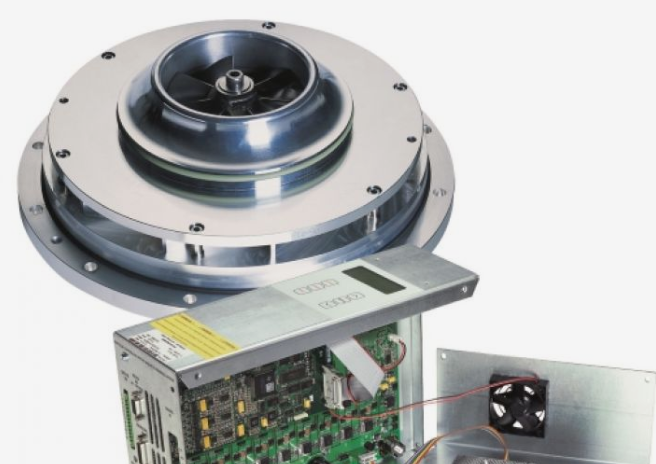
\includegraphics[height=4cm]{1-Mecos.png}}\quad
  \subfloat[Calnetix公司余热回收发电系统]{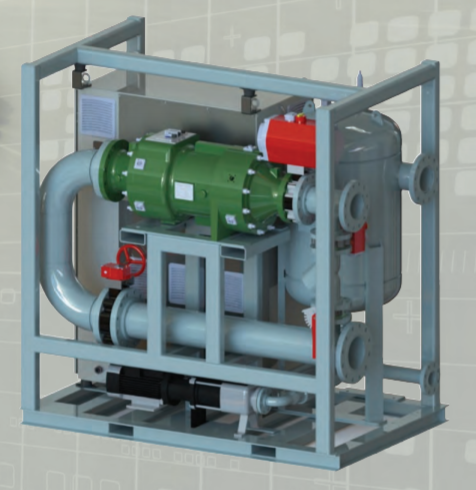
\includegraphics[height=4cm]{1-Calnetix.png}}\quad
  \subfloat[SKF公司污水处理厂通用鼓风机系统]{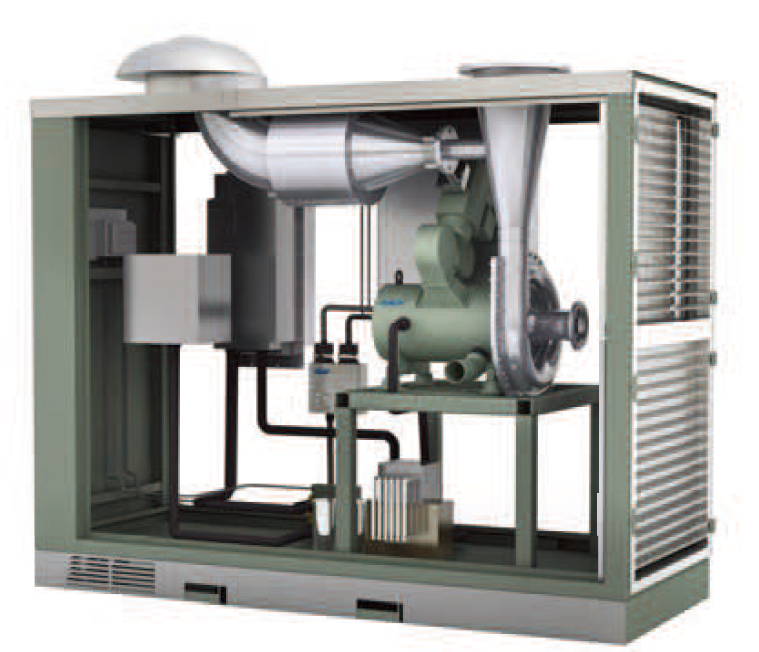
\includegraphics[height=4cm]{1-Skf.png}}\quad  
  \caption[国外磁悬浮电机的应用]{国外磁悬浮电机的应用\label{fig:industrial_amb}}
\end{figure}

工业领域磁悬浮技术已经成熟发展。瑞士Mecos公司、美国Calnetix公司和Waukesha公司、瑞典的SKF公司、加拿大的REVOLVE公司、法国的S2M公司(现已被SKF收购)、德国的LEViTEC公司、芬兰的High Speed公司、俄罗斯的OKBM和日本的精工在磁悬浮的商业应用上占据主流市场地位。\autoref{fig:industrial_amb}~是Mecos公司2019年在售产品二氧化碳鼓风机,二氧化碳用作某些新能源发电场合的冷却介质,二氧化碳鼓风机用于产生高速气流。该鼓风机电机功率15千瓦,稳定运行速度可达54000转/分。Calnetix公司的余热回收发电系统如\autoref{fig:industrial_amb}~所示,其中磁悬浮发电机发电功率可达125千瓦,电机转速可达26500转/分。SKF公司为污水处理厂通用鼓风机系统提供75至350千瓦功率的磁悬浮无油电动机解决方案如\autoref{fig:industrial_amb}~所示,其电动机转子转速可达40000转/分,转子位移采集频率可达15千赫兹。

\begin{figure}[h!]
  \subfloat[飞旋科技磁悬浮复合分子泵]{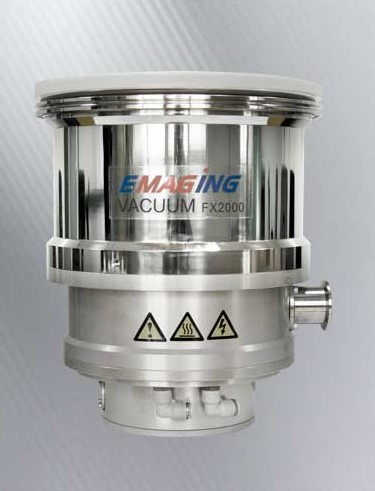
\includegraphics[height=6cm]{1-Feixuan.jpg}}\quad
  \subfloat[磁之汇磁悬浮轴承控制器]{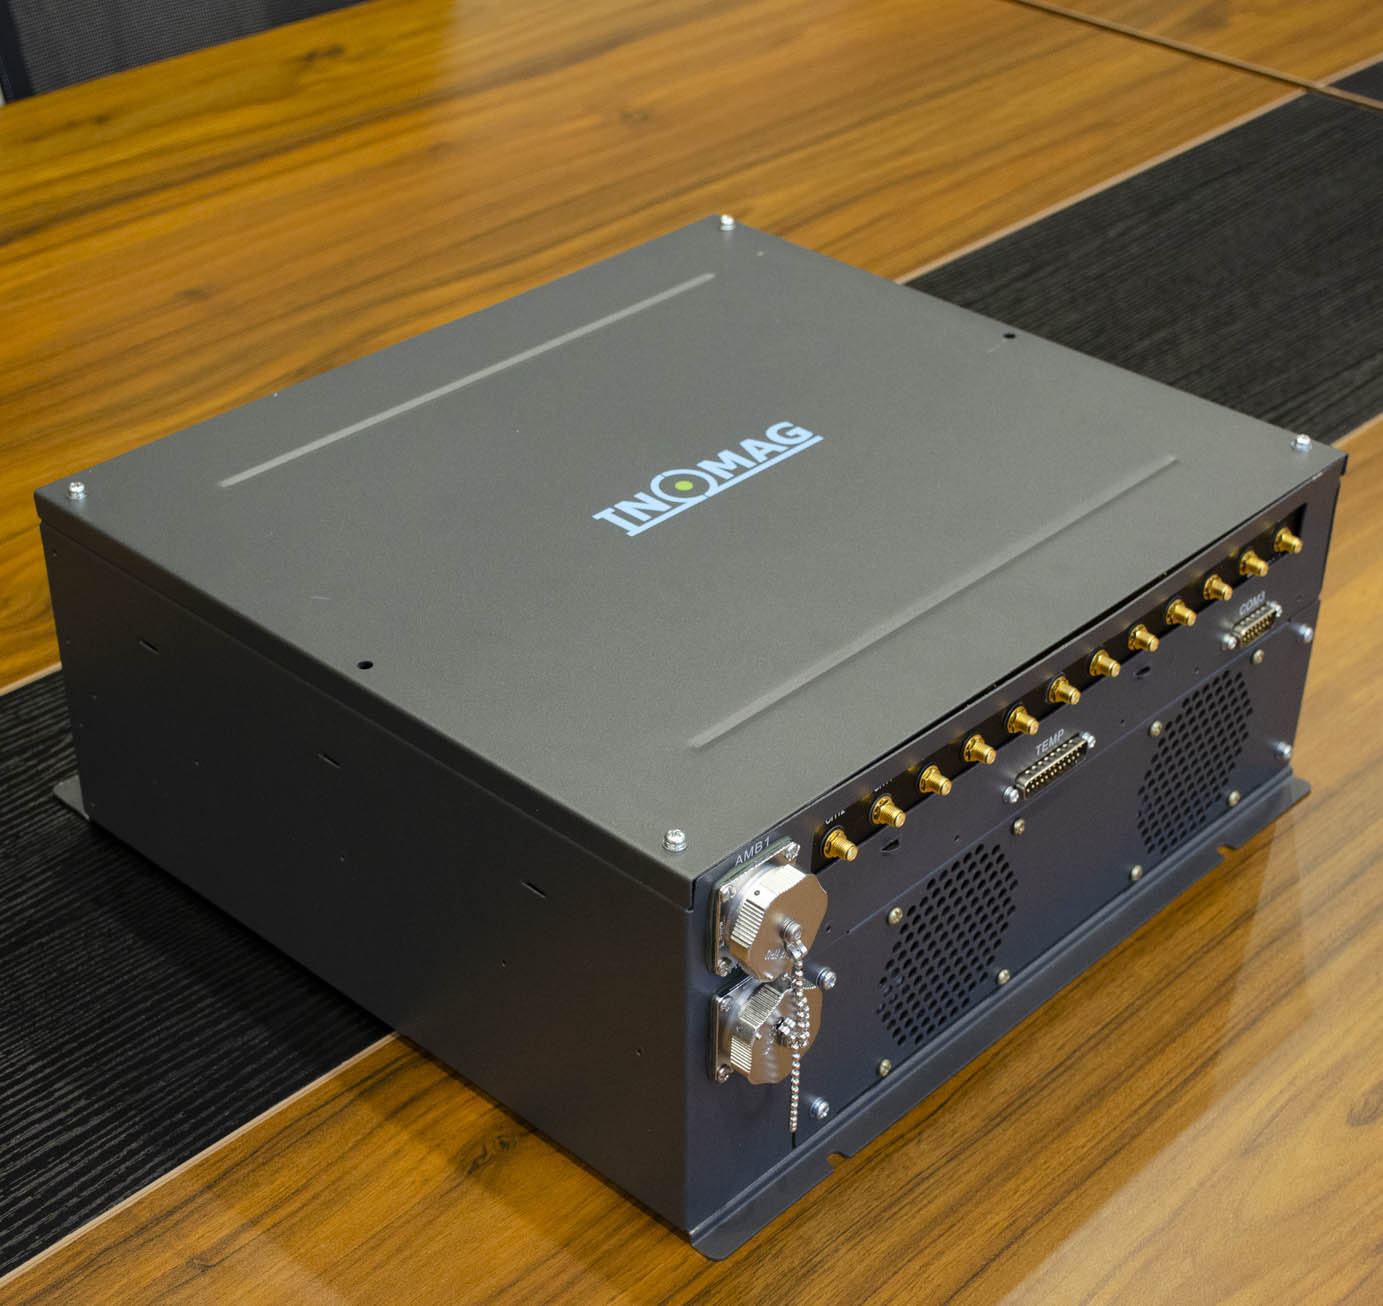
\includegraphics[height=6cm]{1-cizhihui.jpg}}\quad
  \subfloat[磁谷科技磁悬浮离心式鼓风机]{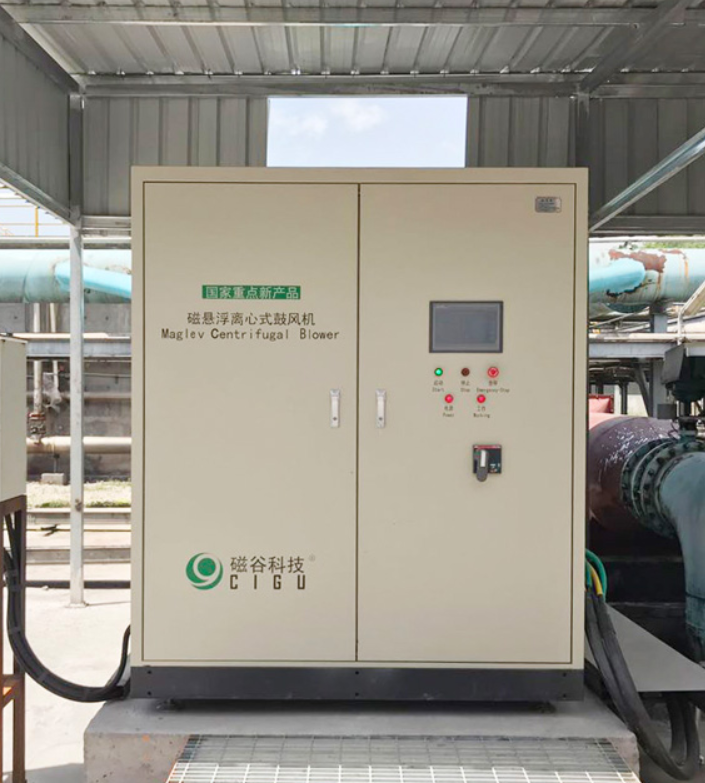
\includegraphics[height=6cm]{1-Cigu.png}}\quad
  \caption[国内磁悬浮电机的应用]{国内磁悬浮电机的应用\label{fig:industrial_amb_cn}}
\end{figure}

国内磁悬浮轴承技术商用成熟的公司有天津飞旋科技、南京磁之汇电机有限公司和南京磁谷科技。天津飞旋科技由清华大学的技术团队创立,现已有商用产品磁悬浮复合分子泵、磁悬浮高速永磁同步电机和磁悬浮离心鼓风机等;南京磁之汇电机有限公司由南京航空航天大学的技术团队创立,研制产品有磁悬浮压缩机。南京磁谷科技的磁悬浮离心式鼓风机进口流量可达280立方米/分,已应用在多种场合。上述产品如\autoref{fig:industrial_amb}~所示。国内磁悬浮电机市场正处于高速发展时期,如何将学术界的研究成果转换应用在工业领域,充分发挥磁悬浮技术的节能、清洁优势,是目前行业同仁共同致力解决的问题。

\section{磁悬浮轴承振动抑制技术研究现状}
理想情况下,转子位于轴承中心位置绕自身几何轴旋转,轴线绕组中的控制电流仅含有直流分量用于克服外界恒定作用力,如转子自身重力。而实际系统中,电流中往往不仅包含直流分量,也含有周期性的交流分量。该交流分量导致磁轴承对转子施加周期性磁场力,进而使基座受到同频反作用力,由此产生振动力。

磁轴承的不平衡控制目标有三类。第一类是实现零电流控制:线圈中的控制电流为交流分量为零,则系统可以实现最低电力功耗,但是残余的位移刚度仍会引起部分残余的不平衡振动力;第二类是实现零力控制:控制磁轴承电磁力的交流分量为零,此状态下可以实现最低振动力为零,但是此时控制电流交流分量幅值不为零;第三类是零位移控制:控制转子的旋转轴与几何轴重合,达到高回转精度的要求,但是会加剧振动力。

第一类和第二类控制目标适用于动力传动领域,如鼓风机或压缩机,此类应用场合往往对转子的回转精度要求不高,而要求整机功耗或振动力越小越好;第三类控制目标适用于机械加工领域,如机床加工电主轴,此类应用场合要求转子具有非常高的回转精度,以满足高精度加工需求。磁悬浮空气压缩机转速高、功耗大,控制目的是降低功耗以及降低振动,因此本文的不平衡振动的控制目标是第一类或第二类。

实际工作状况下, 磁悬浮轴承支承的空气压缩机转子在额定转速范围内高速旋转,转子不平衡带来的振动大幅增加了系统的功耗、降低了系统的稳定性,并且带来的噪声污染问题。因此,研究如何抑制磁悬浮轴承振动具有重要意义。

磁悬浮轴承中的振动主要来源是转子质量不平衡、传感器偏差和磁极偏差。转子质量不平衡是指由于机械加工的工艺限制,转子的几何轴和惯性轴不重合,由此使得旋转轴介于几何轴和惯性轴之间,引起与转速同频的振动力;传感器偏差是指被传感器检测的转子表面为非理想圆形,且检测面材料不均匀会在测量得到的位移信号中引入同频或者倍频信息,引起同频或倍频振动力;磁极偏差是指径向磁极对称中心与转子旋转中心不重合,该因素影响较小,通常可忽略不计。

许多文献针对磁悬浮轴承中的同频振动问题做了深入研究。1983年,Burrows通过开环控制的方式抑制转子不平衡位移响应,实现不平衡补偿,该方法依赖于转子不平衡响应数据以及影响矩阵T\cite{burrows1983vibration}。1989年,Burrows在其前文研究基础上加入自适应环节,实现最优矢量自动更新\cite{burrows1989active}。1993年,Knospe在Burrows方法的基础上采用自适应方法,进一步研究了影响系数矩阵T在线生成\cite{knospe1993adaptive}。1994年,N., Taguchi提出自适应反馈补偿方法自动平衡或不平衡补偿,同频补偿信号注入到控制回路中实现零位移或者零力控制,该方法的缺点是无法从理论上证明收敛性\cite{taguchi1994unbalance}。1995年,Mohamed提出使用Q-parameterization方法实现自动平衡\cite{mohamed1995imbalance}。1996年,Herzog提出通用陷波器实现自动平衡,该方法基于闭环系统设计,且通过测量系统的输出敏感度函数、无需精准的系统参数模型,具有参数设计流程简单,且可以保持原闭环系统的稳定性的优点,该方法后被广泛引用并研究\cite{herzog1996unbalance}。1996年,Matsumura使用H无穷控制策略实现自动平衡\cite{matsumura1996application}。1997年,HS Na在不改变环路的稳定性的条件下,插入最小均方(Least Mean Square,简称LMS)滤波器抑制不平衡振动位移,实现不平衡补偿\cite{na1997adaptive}。2004年,J.Shi使用自适应方法实现自动平衡,控制器的稳定性是靠不断更新参数来实现的\cite{shi2004synchronous}。2005年,Chao使用时域迭代学习控制和增益调度方法,实现自动平衡,它使用跟随转速变化学习周期和学习增益来达到系统的稳定\cite{bi2005automatic}。2006年,Matras引入模型参考自适应方法, 可解决MIMO(Multiple Input Mulpiple Output,简称MIMO)耦合问题。其基本思想是令一扰动输入的对象, 通过自适应方法跟踪一无扰动输入的参考模型, 以抑制对输入扰动的响应。仿真与实验结果证明, 对频率已知、持续稳定的正弦激励, 即便幅值未知、且随时间发生改变, 该方法仍有效。缺点是在应用过程中,参数中的权重阵选取很关键, 且算法收敛速度较慢\cite{matras2006suppression}。2006年,彭晓军提出约束条件更加严格的通用陷波器设计方法\cite{彭晓军2006磁电轴承中抑制不平衡振动的陷波滤波器设计方法},补充1996年通用陷波器设计未考虑“低阻尼振荡现象”的问题。2007年,Vahedforough提出改进的自适应不平衡控制方法,该方法采用两个自适应观测器,实现自动平衡\cite{vahedforough2007estimation}。2012年,徐向波提出了一种基于相移通用陷波反馈控制的同频电流抑制方法,可有效抑制控制器、功放系统产生的同频电流,实现自动平衡\cite{xu2012stability}。2014年,缪存孝在2012年徐向波的研究基础上,考虑感应电动势,抑制同频电流\cite{缪存孝2014含转子不平衡的磁轴承建模与同频电流抑制}。2015年,崔培玲采用相移陷波器,以同频振动力为控制目标,消除同频振动力,实现自动平衡\cite{崔培玲2015基于相移陷波器的磁轴承不平衡振动全频自适应控制}。2016年,彭聪提出谐振控制器解决传统控制策略不是针对时变转速的问题,以及针对时变转速但是控制器结构复杂的问题,该方法补偿掉位移负刚度,实现自动平衡\cite{peng2016synchronous}。2017年,彭聪提出使用多谐振控制器抑制基波和谐波电流,实现自动平衡\cite{peng2016frequency}。

另一方面,针对位移传感器引入的倍频扰动问题,亦有许多文献做了相关的研究。第一类控制方法是将多个针对单一频率的振动抑制器连接在一起。Mahdi Darbandi将多个陷波器组合来消除谐波电流,同时根据系统的输出敏感度函数曲线来设计陷波器参数,以保证闭环系统稳定性\cite{mahdi2017harmonic}。然而,当需要一直的谐波频率数量较多时,需要组合多个陷波器,由此使得计算负担迅速加大。重复控制器具有单路结构消除多种频率扰动的能力,适合谐波抑制场合。重复控制器早期应用于电源系统中以消除跟踪误差\cite{zhou2008plug},徐向波将重复控制器应用在磁悬浮轴承控制中,消除了控制电流中的谐波成分\cite{xu2015model}。崔培玲改进了重复控制器的结构,将重复控制器的低通滤波器移动至延时环路之外,由此得到了更好的电流谐波抑制效果\cite{cui2016suppression}。周克亮提出奇数次重复控制器的应用方法,其应用场合是PWM变换器\cite{zhou2006zero}。但磁悬浮轴承是开环不稳定结构,奇数次重复控制器不能直接从PWM变换器移植到磁悬浮轴承的控制回路中。如何在磁悬浮轴承中应用重复控制器——理论推导、稳定性分析、参数设计仍是有待深入研究的问题。

除上述提到的针对同频和倍频扰动的主动控制抑制方法,还有使用现场动平衡技术的同频振动抑制方法。主动振动抑制方法无法同时实现零电流或者零位移控制,这是因为闭环控制之下,无法通过调节控制器参数同时实现减小轴承刚度和增大轴承刚度。动平衡技术校正不平衡质量,可以从源头上除去同频扰动,进而达到既抑制电流同频成分,又抑制位移同频成分的目的。传统的动平衡借助动平衡机完成,该方法需要将电机转子单独放置在动平衡机上,通过增重或去重完成转子不平衡质量校正之后再装回电机。然而磁悬浮转子进行动平衡时,动平衡机的轴承系统与磁悬浮电机的轴承系统不一定重合,由此会引入校正误差,导致即使在动平衡机上达到了良好的校正效果,转子在工况下旋转时仍有残余不平衡质量。借助磁悬浮可主动控制的特性,磁悬浮电机的转子动平衡过程可以在电机本体内完成,无需拆装转子,此过程称之为现场动平衡。影响系数法和模态平衡法是比较常用的现场动平衡方法,影响系数法是基于假设控制系统是线性的前提,通过多轮试重得到校正质量\cite{john2009relationship,ranjan2019application}。模态平衡法是先构建转子的有限元模型,然后通过实际的振动响应曲线来校正有限元模型。这两种方法的缺点是都需要多轮试重和振动响应测试\cite{wang2014field}。为了简化动平衡操作过程、降低时间消耗,近年来一些文献相继提出多种无需试重的现场动平衡方法。该方法可分为两大类:一、抑制不平衡振动位移,使转子旋转轴趋于几何轴,通过转子的控制电流辨识不平衡质量矢量\cite{fang2013field,liu2015field}。二、抑制不平衡振动力,使转子旋转轴趋于惯性轴,通过转子的位移辨识不平衡质量矢量\cite{xu2015field}。上述控制方法均需要抑制电流或位移中的交流分量,以达到控制转子旋转轴的目的。然而,以上文献仅关注了同频扰动成分的抑制,没有考虑倍频扰动成分的抑制,因此对不平衡质量的辨识结果准确度有限。

\section{本文的研究工作和安排}
本文以抑制磁悬浮轴承系统中振动力为控制目标,分析了磁悬浮轴承系统的控制原理和振动模型,提出了一套组合方案来抑制振动,并在磁轴承数字控制平台上完成仿真和实验验证。本文具体的研究内容安排如下:

第一章介绍了磁悬浮电机的发展和应用现状,分析了国内外对磁悬浮轴承技术的研究发展。对同频和倍频振动抑制方法、重复控制器和现场动平衡技术的研究现状做了详尽的调研。

第二章研究了磁悬浮系统的工作原理,建立了磁悬浮轴承支撑的刚性转子动力学模型和考虑质量不平衡和传感器位移误差在内的磁悬浮系统的振动模型,进行了输出敏感度实验验证了控制器性能的可靠性。

第三章针对磁悬浮轴承中质量不平衡和传感器误差引起的同频和倍频振动,分析了使用传统重复控制器(Conventional Repetitive Controller,简称CRC)来抑制振动的原理。针对CRC方法的不足,本文提出了零相移奇数次重复控制器(Zero-phase Odd-harmonic Repetitive Controller,简称ZORC)控制方案,阐述了该方法稳定性分析方法和参数设计步骤,通过仿真和实验验证了ZORC的有效性与优越性。

第四章针对主动振动抑制方法无法同时实现振动位移最小和振动力最小的问题,提出使用基于ZORC的现场动平衡方法,进一步抑制质量不平衡引起的同频振动。分析了该方法的原理与实际操作流程,通过实验验证了该方法的有效性。

第五章介绍了磁悬浮轴承数字控制平台的实验方案设计。介绍了硬件模块和软件设计流程,包括软件主要组成部分的设计。

第六章总结了全文的研究内容,提出了下一步的工作展望。

\chapter{磁悬浮系统和振动模型}
本章分析磁悬浮轴承系统的硬件结构和软件控制原理。将转子视为刚体,建立其径向四自由度的广义坐标系模型。考虑质量不平衡和传感器误差因素,分析并建立转子振动模型。

\section{磁悬浮系统工作原理}
本文研究的磁悬浮电机为磁悬浮离心压缩机,它是由一个永磁同步电机和分立在两端的两套轴向径向磁轴承组成,结构如\autoref{fig:2-1-structure}~所示。其中校正盘A和校正盘B处设计为叶轮安装位置,本文第三章实验中该位置处安装叶轮,第四章实验中安装校正盘。该磁悬浮离心压缩机的电气参数如\autoref{tab:motor_para}~所示。由于转子额定转速远低于其一阶弯曲频率,因此可以将转子视为刚性转子,本文分析转子刚性模态下的动力学模型和振动力模型。

\begin{figure}[h!]
	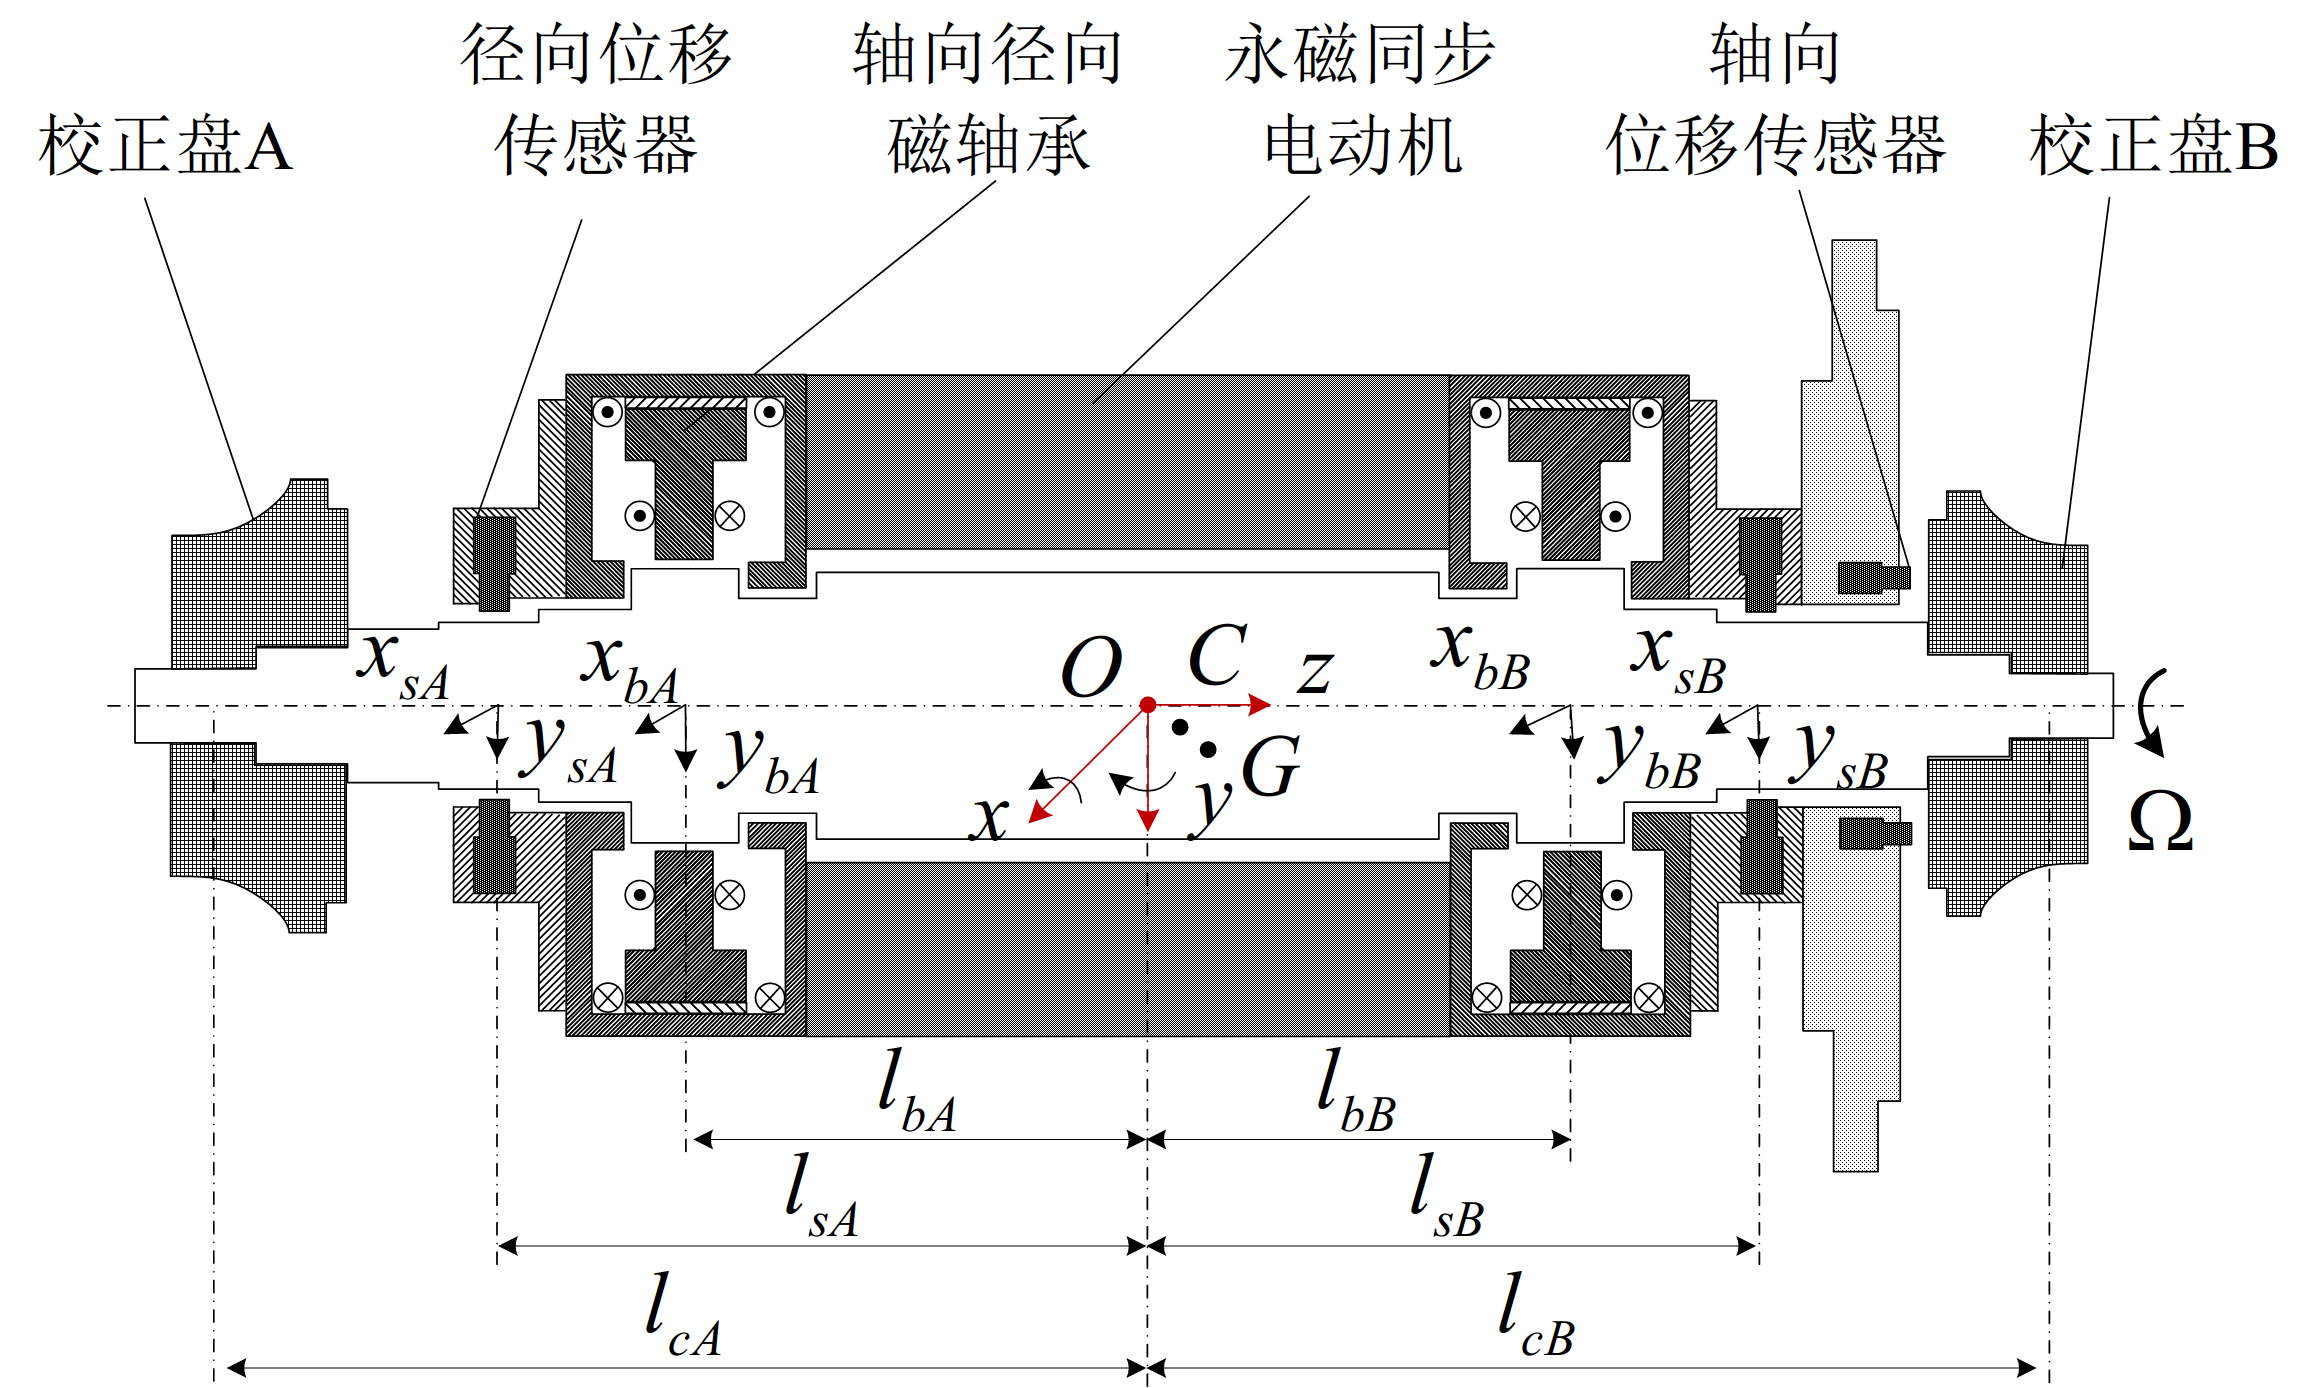
\includegraphics[scale=1.0]{2-1-structure.png}
	\caption{磁悬浮离心压缩机结构示意图}
	\label{fig:2-1-structure}
\end{figure}

\begin{table}[h!]
  \caption[磁悬浮离心压缩机电气参数]{磁悬浮离心压缩机电气参数\label{tab:motor_para}}
  \begin{tabular}{cc}
    \toprule
    物理量 & 值 \\
    \midrule
    额定功率 & 7.5kW\\
    额定转速 & 833Hz\\
    转子一阶弯曲频率 & 1589Hz\\
    \bottomrule
  \end{tabular}
\end{table}

笛卡尔坐标系下,空间中的刚体存在六个方向上的运动:三个坐标轴方向上的平动以及绕三个坐标轴的转动,称之为六个自由度。磁悬浮离心压缩机中,两端组合的轴向径向磁轴承可以约束转子其中五个自由度的运动,余下一个自由度的转动由电机驱动器控制。

磁悬浮轴承控制的目标是使转子在电机未旋转或电机以额定转速旋转时,均稳定悬浮在两端磁轴承中心,不与保护轴承接触。磁悬浮轴承和转子组成的系统是一个开环不稳定的控制系统,需要引入闭环控制才能使其保持稳定。磁悬浮轴承闭环控制系统由数字信号处理器、位移传感器和功率放大器组成:

位移传感器实时高频采集转子位置,目前磁悬浮轴承中位移传感器的采样频率可达100kHz。通常位移传感器信号经降噪滤波等调理电路处理后输入到数字信号处理器中。高灵敏度、线性度和足够的带宽是传感器实时可靠获取转子位置的必要保障。

常用的数字信号处理器有DSP(Digtal Signal Processor,简称DSP),如TMS320F28335。近年来以Cortex-M4为核心的单片微处理器亦配备充足的计算能力,如STM32F4系列单片机。数字信号处理器是磁轴承控制系统的枢纽,其根据位移传感器采集的信号,向下级输出给定磁悬浮力。高速的运算能力保证各类控制算法如PID调节器、滤波器等的得以被部署运行。

功率放大器和磁轴承线圈共同组成磁轴承系统的执行元件。变化的转子位置经使数字信号处理器采样和运算后输出不同的给定电流。给定电流经功率放大器调理,在磁轴承线圈中产生控制电流,最终输出磁悬浮力控制转子的位置。

\section{磁悬浮转子动力学模型}
\autoref{fig:2-1-structure}~中,记转子的几何中心为$ G $,质量中心为$ C $,$ l_{bA} $和$ l_{bB} $表示A端和B端轴向径向磁轴承到转子几何中心的距离,$ l_{sA} $和$ l_{sB} $表示A端和B端位移传感器到转子几何中心的距离,$ l_{cA} $和$ l_{cB} $表示A端和B端质量校正盘到转子几何中心的距离。以磁轴承中心为原点建立广义坐标系$ O-xyz $,原点记为$ O $。转子绕$ x $和$ y $轴的旋转角度分别记为$ \alpha $和$ \beta $。转子的旋转速度记为$ \Omega $。

定义转子质量中心$ C $在$ O-xyz $中的运动位移为${\textbf{\textit{q}}_i} = {\left[ {{\beta _i},{x_i}, - {\alpha _i},{y_i}} \right]^T}$,转子几何中心$ G $在$ O-xyz $中的运动位移为${\textbf{\textit{q}}_g} = {\left[ {{\beta _g},{x_g}, - {\alpha _g},{y_g}} \right]^T}$,转子在两端位移传感器截面处的位移记为${\textbf{\textit{q}}_s} = {\left[ {{x_{sA}},{x_{sB}},{y_{sA}},{y_{sB}}} \right]^T}$,转子在两端磁轴承截面处的位移记为${\textbf{\textit{q}}_b} = {\left[ {{x_{bA}},{x_{bB}},{y_{bA}},{y_{bB}}} \right]^T}$。

由于转子在$ O-z $轴上的平动与$ O-x $和$ O-y $上的运动可视为解耦,因此轴向运动与径向运动可分开控制。本小节研究转子在径向上的动力学模型。$ \textbf{\textit{q}}_{b} $,$ \textbf{\textit{q}}_{g} $和$ \textbf{\textit{q}}_{s} $可以通过线性变换互相得到:
\begin{equation}
\label{eq2-1}
{\textbf{\textit{q}}_b} = {\textbf{\textit{B}}^T}{\textbf{\textit{q}}_g}
\end{equation}
\begin{equation}
\label{eq2-2}
{\textbf{\textit{q}}_s} = \textbf{\textit{C}}{\textbf{\textit{q}}_g}
\end{equation}
其中,
${\textbf{\textit{B}}} = \left[ {\begin{array}{*{20}{c}}
{ - {l_{bA}}}&{{l_{bB}}}&0&0\\
1&1&0&0\\
0&0&{ - {l_{bA}}}&{{l_{bB}}}\\
0&0&1&1
\end{array}} \right]$,
${\textbf{\textit{C}}} = \left[ {\begin{array}{*{20}{c}}
{ - {l_{sA}}}&{1}&0&0\\
{l_{bB}}&1&0&0\\
0&0&{ - {l_{bA}}}&{1}\\
0&0&{l_{bB}}&1
\end{array}} \right]$。

磁悬浮轴承中的磁悬浮力取决于定子和转子之间的磁场强度,而磁场强度与线圈中的控制电流和气隙长度相关,磁悬浮力$ {f_m} $可以通过转子位移和控制电流线性表示为
\begin{equation}
\label{eq2-3}
{f_m} = {k_s}x + {k_i}i
\end{equation}
其中${k_s}$为位移刚度,${k_i}$为电流刚度。根据牛顿运动定律,转子的动力学方程即可以表示为
\begin{equation}
\label{eq2-4}
\boldsymbol{M} \ddot{\boldsymbol{q_i}} + \boldsymbol{G}\dot{\boldsymbol{q_i}} =  - \boldsymbol{B}\boldsymbol{K_s} {\boldsymbol{B}}^T \boldsymbol{q_i} + \boldsymbol{B} \boldsymbol{K_i} \boldsymbol{i}
\end{equation}
其中质量矩阵$\boldsymbol{M}$、反对称陀螺矩阵$\boldsymbol{G}$、位移刚度矩阵$\boldsymbol{K_s}$、电流刚度矩阵$\boldsymbol{K_i}$和控制电流矩阵$i$可分别表示为

$$\boldsymbol{M} = \left[ {\begin{matrix}
   {{I_y}} & 0 & 0 & 0  \cr 
   0 & m & 0 & 0  \cr 
   0 & 0 & {{I_x}} & 0  \cr 
   0 & 0 & 0 & m  \cr 
 \end{matrix} } \right]$$,
 
$$\boldsymbol{G} = \Omega \left[ {\begin{matrix}
   0 & 0 & {{I_z}} & 0  	\\
   0 & 0 & 0 & 0  			\\ 
   { - {I_z}} & 0 & 0 & 0  	\\ 
   0 & 0 & 0 & 0  			\\ 
 \end{matrix} } \right]$$

$$\boldsymbol{K_s} = \left[ {\begin{matrix}
   {{K_{sA}}} & 0 & 0 & 0  \cr 
   0 & {{K_{sB}}} & 0 & 0  \cr 
   0 & 0 & {{K_{sA}}} & 0  \cr 
   0 & 0 & 0 & {{K_{sB}}}  \cr 

 \end{matrix} } \right]$$

$$\boldsymbol{K_i} = \left[ {\begin{matrix}
   {{K_{iA}}} & 0 & 0 & 0  \cr 
   0 & {{K_{iB}}} & 0 & 0  \cr 
   0 & 0 & {{K_{iA}}} & 0  \cr 
   0 & 0 & 0 & {{K_{iB}}}  \cr 

 \end{matrix} } \right]$$

$$\boldsymbol{i} = \left[ {\begin{matrix}
   {{i_{xA}}} & 0 & 0 & 0  \cr 
   0 & {{i_{xB}}} & 0 & 0  \cr 
   0 & 0 & {{i_{yA}}} & 0  \cr 
   0 & 0 & 0 & {{i_{yB}}}  \cr 

 \end{matrix} } \right]$$
本文研究的磁悬浮离心压缩机中的磁悬浮轴承是对称设计结构,因此两端的三自由度磁悬浮轴承的位移刚度和电流刚度是一样的,即$ks_A = k_{sB} = k_s$,$k_{iA} = k_{iB} = k_i$。$ I_x $、$ I_y $和$I_z$分别表示转子绕$ x $轴、$ y $轴和$ z $轴的惯性力矩。该磁悬浮轴承及控制系统相关参数如下:
\begin{table}[htb]
  \caption[磁悬浮离心压缩机中磁悬浮轴承系统参数]{磁悬浮离心压缩机中磁悬浮轴承系统参数\label{tab:bearing_para}}
  \begin{tabular}{cc}
    \toprule
    物理量 & 值 \\
    \midrule
    $l_{bA} = l_{bB}$ & $0.08m$ \\
    $l_{sA} = l_{sB}$ & $0.12m$ \\
    $l_{cA} = l_{cB}$ & $0.14m$ \\
    $m$	  & $3.9kg$ \\
    $k_s$ & $-2.38\times 10^5N/m$\\
    $k_i$ & $67.0N/A$\\
    $f_s$ & $12.5kHz$\\   
    \bottomrule
  \end{tabular}
\end{table}



\section{磁悬浮系统振动模型}
\subsection{转子质量不平衡}
\begin{figure}[h!]
	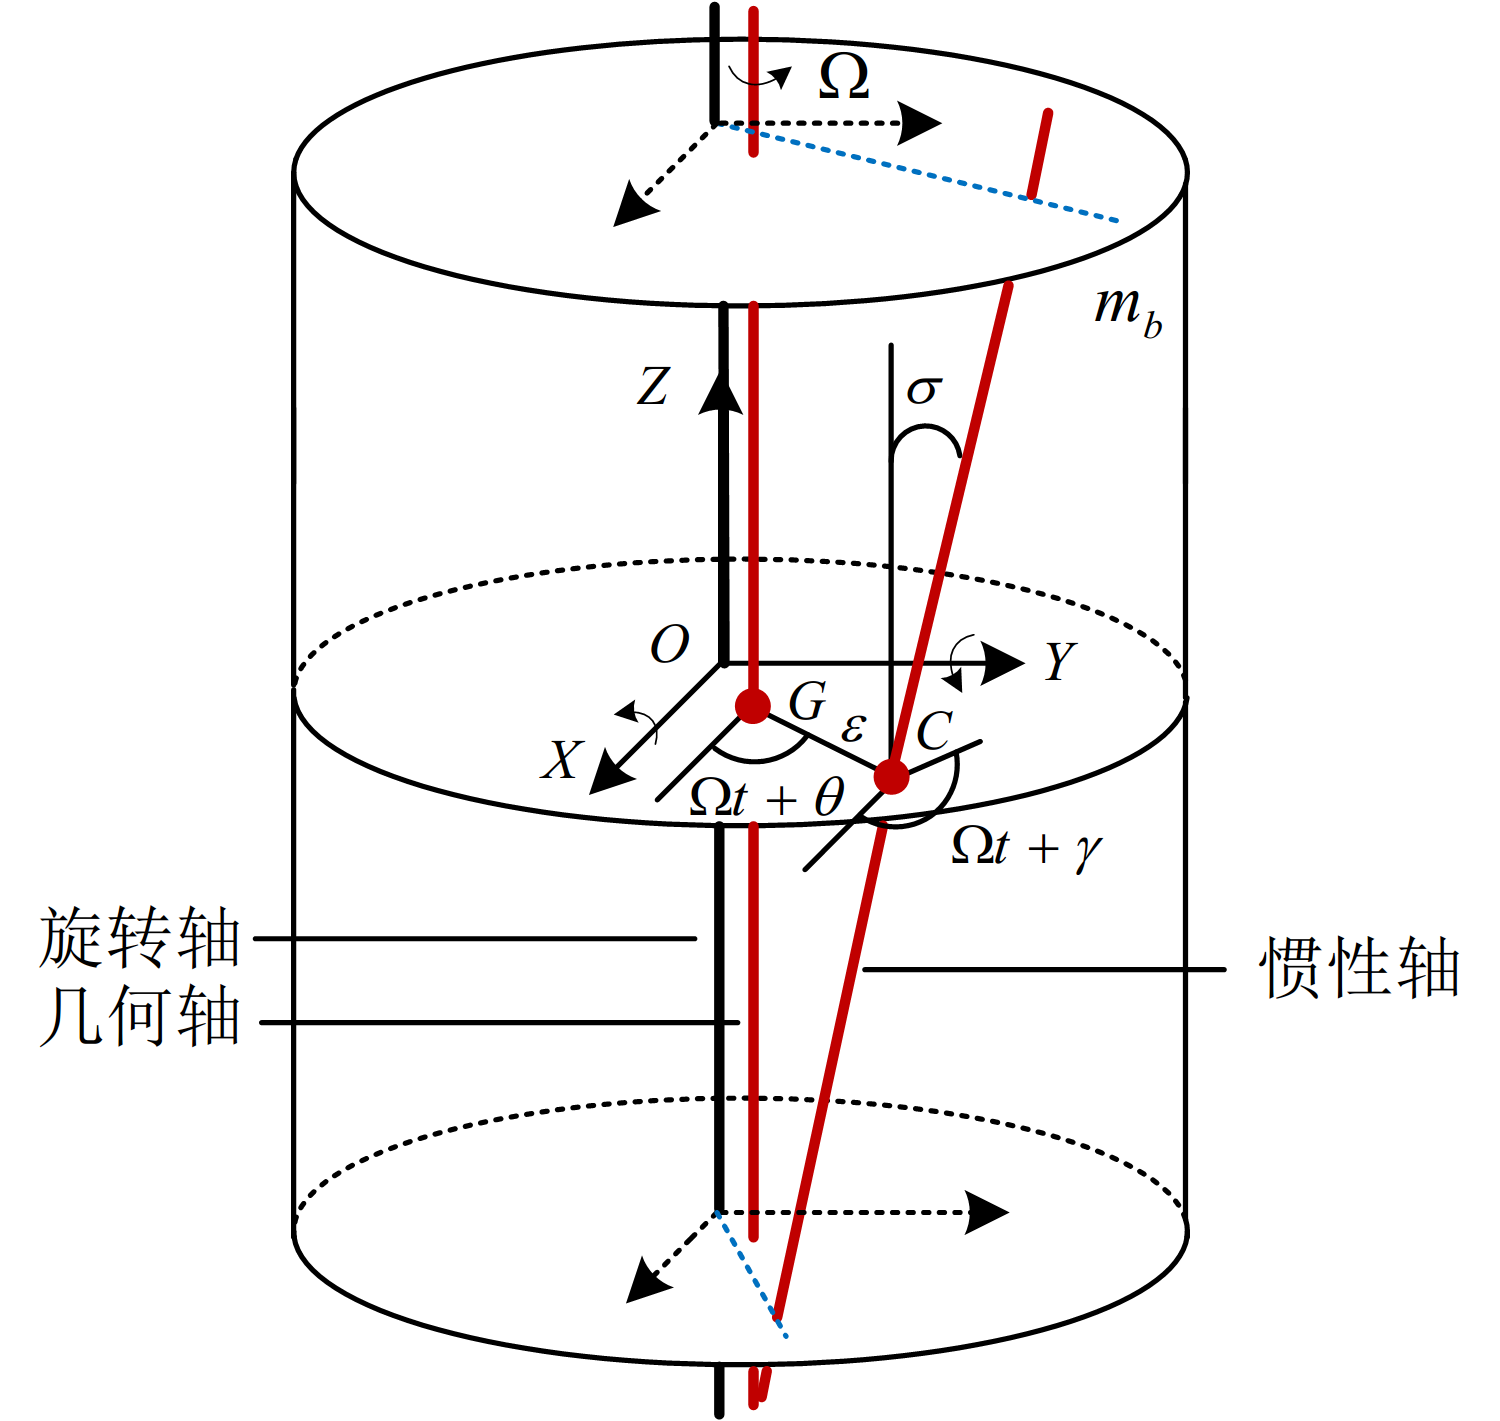
\includegraphics[scale=1.0]{2-2-unbalance.png}
	\caption{转子质量不平衡造成几何轴和惯性轴偏离旋转轴}
	\label{fig:2-2-unbalance}
\end{figure}

转子的不平衡质量造成其几何轴、惯性轴和旋转轴不重合,即质量中心(即惯性轴中心)$ \boldsymbol{q_i} $和几何中心(即几何轴中心)$ \boldsymbol{q_g} $发生偏离。不平衡质量造成转子静不平衡和动不平衡:静不平衡指几何轴与惯性轴在同一平面上的偏移,在转子旋转时产生振动力;动不平衡是指几何轴和惯性轴因角度偏移而异面,在转子旋转时产生振动力矩,如\autoref{fig:2-2-unbalance}~所示。若记该偏移距离为$ \boldsymbol{q_{\Delta}} $,则可以表示
\begin{equation}
\label{eq:q_delta}
\boldsymbol{{q}_\Delta }{ = }\left[ 
{\begin{matrix}
   {\sigma \cos \left( {\Omega t + \gamma } \right)}  \cr 
   {\xi \cos \left( {\Omega t + \theta } \right)}  \cr 
   {\sigma sin\left( {\Omega t + \gamma } \right)}  \cr 
   {\xi \sin \left( {\Omega t + \theta } \right)}  \cr 
\end{matrix}} 
 \right]
\end{equation}
其中$\sigma$表示动平衡的幅值,$\gamma$表示动不平衡的初相位;$\xi$表示静平衡的幅值,$\theta$表示静不平衡的初相位。则几何中心与质量中心的空间关系可以表示为
\begin{equation}
\boldsymbol{{q}_i}{ = }\boldsymbol{{q}_{g}} + \boldsymbol{{q}_\Delta }
\end{equation}

\subsection{位移传感器误差}

\begin{figure}[h!]
	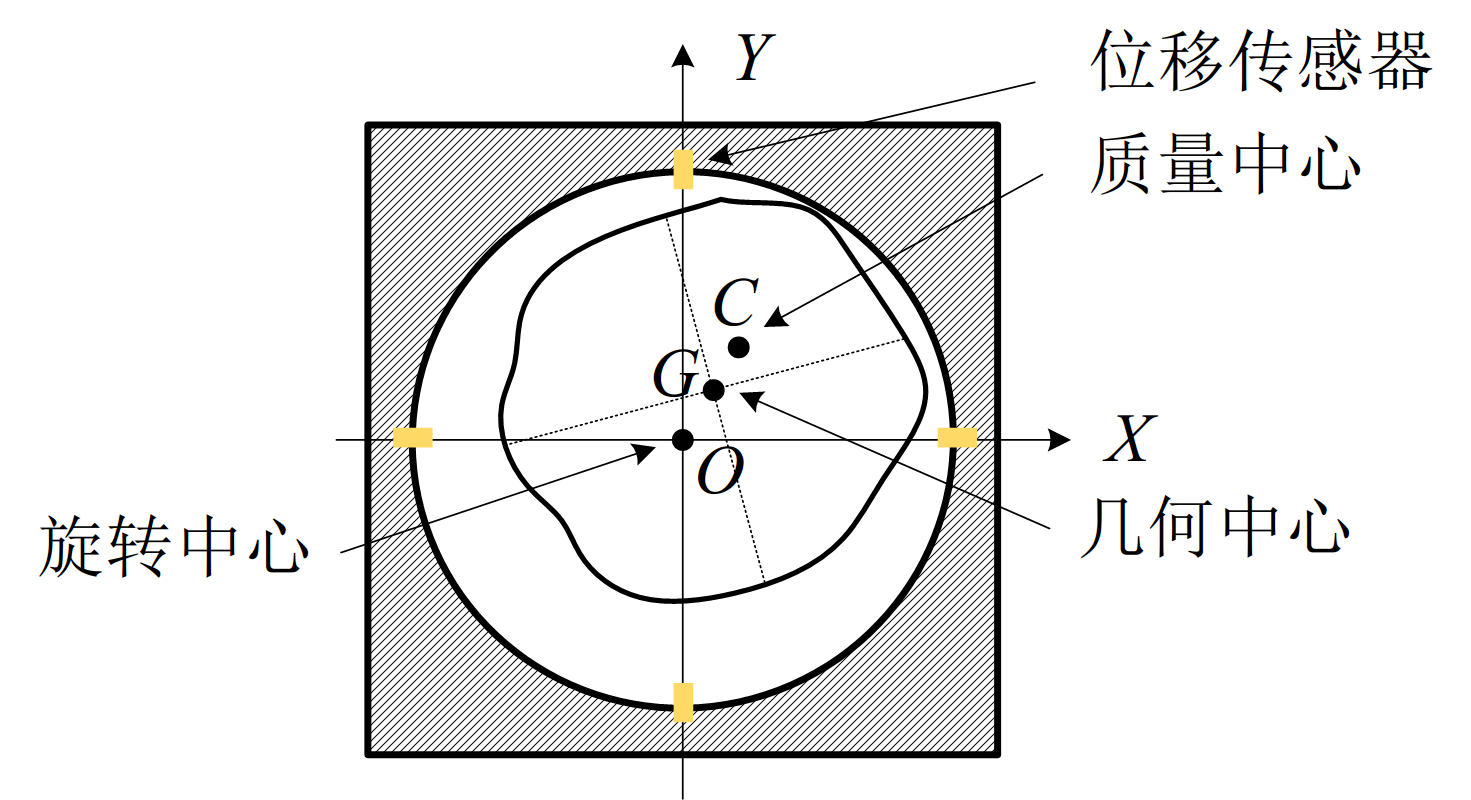
\includegraphics[scale=1.0]{2-3-sensor.png}
	\caption{传感器检测面不均与引起检测误差}
	\label{fig:2-3-sensor}
\end{figure}

三自由度轴向径向磁轴承中,正交方向上的两个自由度的控制分别使用一对位移传感器来检测转子在该磁轴承处的位移,如\autoref{fig:2-3-sensor}~所示。由于实际加工精度限制,转子的位移检测面通常不是一个正规、平滑的圆面,而是凹凸不平的不规则面。因此转子的测量位移信号中包含多种频率的噪声扰动、实际位置无法测得。记扰动信号为
\begin{equation}
\Theta \boldsymbol{{q}_s} = \sum\limits_{k = 1}^n {{A_k}\sin \left( {k\Omega t + {\phi _k}} \right)} 
\end{equation}
其中$k$是谐波次数,$A_k$是第$k$次谐波的幅值,$\phi _k$是第$k$次谐波的初相位。记传感器观测的转子位置为${\hat q}_s$,真实的转子位置为$q_s$,则
\begin{equation}
\boldsymbol{{\hat q}_s} = \boldsymbol{{q}_s} - \Theta \boldsymbol{{q}_s}
\end{equation}

\begin{figure}[h!]
	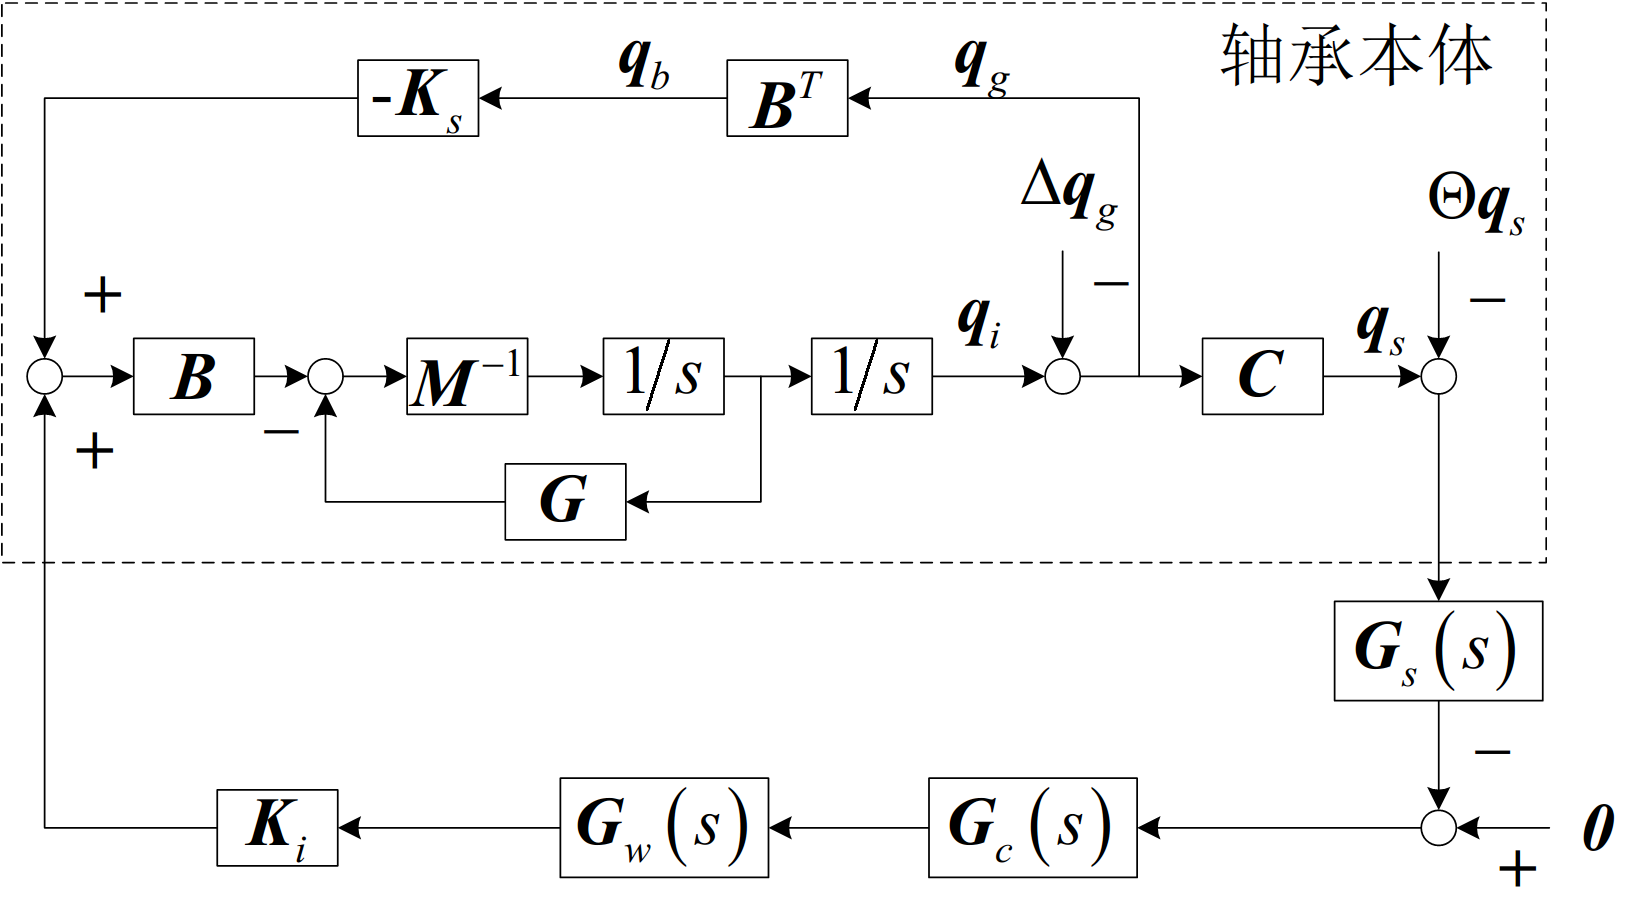
\includegraphics[scale=1.0]{2-4-control.png}
	\caption{磁悬浮轴承系统控制框图}
	\label{fig:2-4-control}
\end{figure}

磁悬浮轴承闭环控制框图如\autoref{fig:2-4-control}~所示。$\boldsymbol{G_s(s)}$是位移传感器的传递函数,$\boldsymbol{G_c(s)}$是PID控制器的传递函数,$\boldsymbol{G_w(s)}$是功率放大器的传递函数。本文采用分散的PID控制策略,即两端三自由度的轴向径向磁轴承分别控制转子在两端的水平和竖直方向的运动,径向共四个控制通道:$XA$、$YA$、$XB$和$YB$。$\boldsymbol{G_s(s)}$、$\boldsymbol{G_c(s)}$和$\boldsymbol{G_w(s)}$均为$4*4$对角矩阵:
$$\boldsymbol{G_w}\left( s \right) = \left[ 
{\begin{matrix}
   {{1 \over {s{f_s} + 1}}} & 0 & 0 & 0  \cr 
   0 & {{1 \over {s{f_s} + 1}}} & 0 & 0  \cr 
   0 & 0 & {{1 \over {s{f_s} + 1}}} & 0  \cr 
   0 & 0 & 0 & {{1 \over {s{f_s} + 1}}}  \cr 

 \end{matrix} }
\right]$$

$$\boldsymbol{G_s}\left( s \right) = \left[ 
{\begin{matrix}
   {{k_{se}}} & 0 & 0 & 0  \cr 
   0 & {{k_{se}}} & 0 & 0  \cr 
   0 & 0 & {{k_{se}}} & 0  \cr 
   0 & 0 & 0 & {{k_{se}}}  \cr 

 \end{matrix} } 
 \right]$$
 
$$\boldsymbol{G_c}\left( s \right) = \left[ {\begin{matrix}
   {{k_p} + {{{k_i}} \over s} + {k_d}s} & 0 & 0 & 0  \cr 
   0 & {{k_p} + {{{k_i}} \over s} + {k_d}s} & 0 & 0  \cr 
   0 & 0 & {{k_p} + {{{k_i}} \over s} + {k_d}s} & 0  \cr 
   0 & 0 & 0 & {{k_p} + {{{k_i}} \over s} + {k_d}s}  \cr 

 \end{matrix} } \right]$$
%考虑质量不平衡和传感器扰动,闭环系统控制方程为

%待补充:位移扰动与PID控制器、控制电流的关系;矩阵方程与单自由度控制的关系;为何轴向和径向视为解耦;考虑扰动时的闭环系统控制方程

\section{磁悬浮轴承控制性能验证}
磁悬浮轴承的轴承刚度和轴承阻尼均可以通过主动控制的方式来调节,然而作为传统机械轴承的替代品,其最应该具备的基本性能是保持稳定,即要求磁悬浮轴承在严苛工况下也能保持支撑转子的能力。数字控制系统中,依据传递函数计算系统特征根位置是主要的系统稳定性分析方法。但是只有获取到准确的参数值,如位移刚度和电流刚度时,根据传递函数解算出的系统特征根才比较准确。实际上理论模型和实际模型很难一致,这是因为电机与轴承加工和装配、位移传感器等系统组件仍会引入一定误差。因此,为验证磁悬浮系统的控制性能,我们需要找到一种便于实际应用且能准确表征系统稳定性能的方法。

磁悬浮轴承ISO 14839-3标准\cite{iso2004mechanical}定义了输出敏感度函数,用于定量分析磁悬浮轴承的稳定性能。定义输出敏感度函数为$S_0$,显示在\autoref{fig:5-sen}~中:
\begin{equation}
	S_0 = \frac{V_2}{V_1}
\end{equation}
其中$G_p$表示磁悬浮轴承本体的传递函数,$G_c$表示控制器的传递函数。注意到
\begin{figure}[h!]
	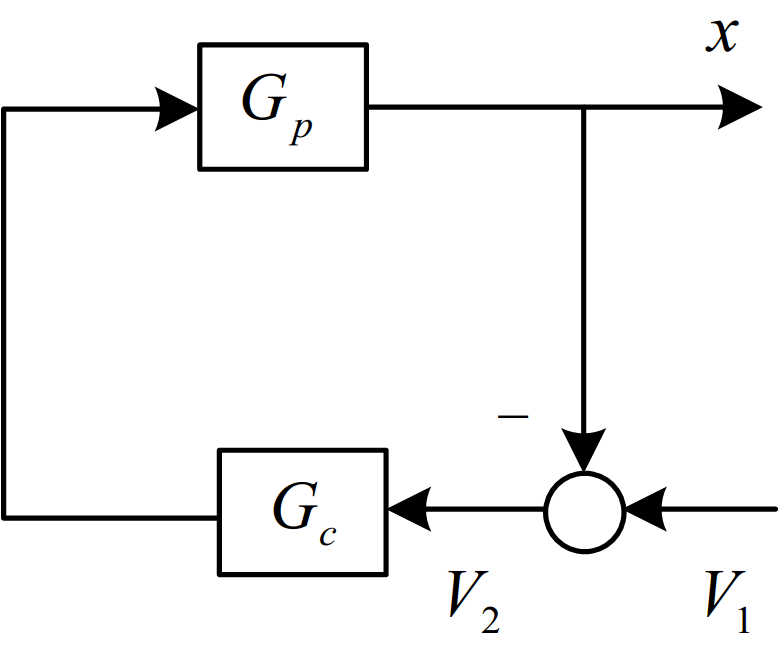
\includegraphics[scale=1.0]{5-sen.png}
	\caption{磁悬浮轴承输出敏感度示意图}
	\label{fig:5-sen}
\end{figure}

\begin{equation}
	S_0(j\omega) = \frac{1}{1 + G_p(j\omega)G_c(j\omega)}
\end{equation}
$1 + G_p(j\omega)G_c(j\omega)$的值越大,则奈奎斯特图上$G_p(j\omega)G_c(j\omega)$与点$(-1,0)$的距离越远,增益裕度越大。那么我们可以通过敏感度函数$S_0(j\omega)$来判定系统增益裕度:敏感度函数$S_0(j\omega)$的峰值越小,增益裕度越大。

敏感度函数测试频率上限通常没有定值,因为敏感度函数超过一定的频率之后,其幅值趋近于1。即随着在敏感度函数测试点注入的激励信号的频率升高,响应点检测的信号幅值会趋近于激励信号本身的幅值。ISO 14839-3标准规定了敏感度函数测试频率的上限为转子额定频率的三倍,但若该值超过2kHz,则取上限为2kHz。

通常磁悬浮轴承控制是采用分散的五自由度独立控制,测试方法为依次在各个通道的测试点上注入激励信号,检测响应信号,得到一个通道的敏感度函数。该过程中其它通道须保持闭环控制。经上述过程测量得到的敏感度函数测量结果可以表示为:
\begin{equation}
	S_{0,max} = max \left[ max_i \left|G_s(j\omega)\right| \right]
\end{equation}
其中频率范围为$\omega = 2 \pi f$,$0 \leq f \leq 2kHz$;测量通道序号为$i$,分别指需要测量的五个自由度。系统的全局稳定性能优劣取决于敏感度函数峰值最大的一个通道。

\begin{table}[h!]
  \caption[ISO 14839-3定义磁悬浮轴承输出敏感度函数峰值稳定区间标准]{ISO 14839-3定义磁悬浮轴承输出敏感度函数峰值稳定区间标准\label{tab:amb_iso}}
  \begin{tabular}{cc}
    \toprule
    输出敏感度函数峰值 & 稳定区间 \\
    \midrule
    $(-\infty,9.5dB]$ & A\\
    $(9.5dB,12dB]$    & B\\
    $(12dB,14dB]$     & C\\
    $(14dB,\infty)$   & D\\
    \bottomrule
  \end{tabular}
\end{table}

\begin{figure}[H]  
	\subfloat[XA控制通道输出敏感度函数曲线\label{fig:5-sens_x}]{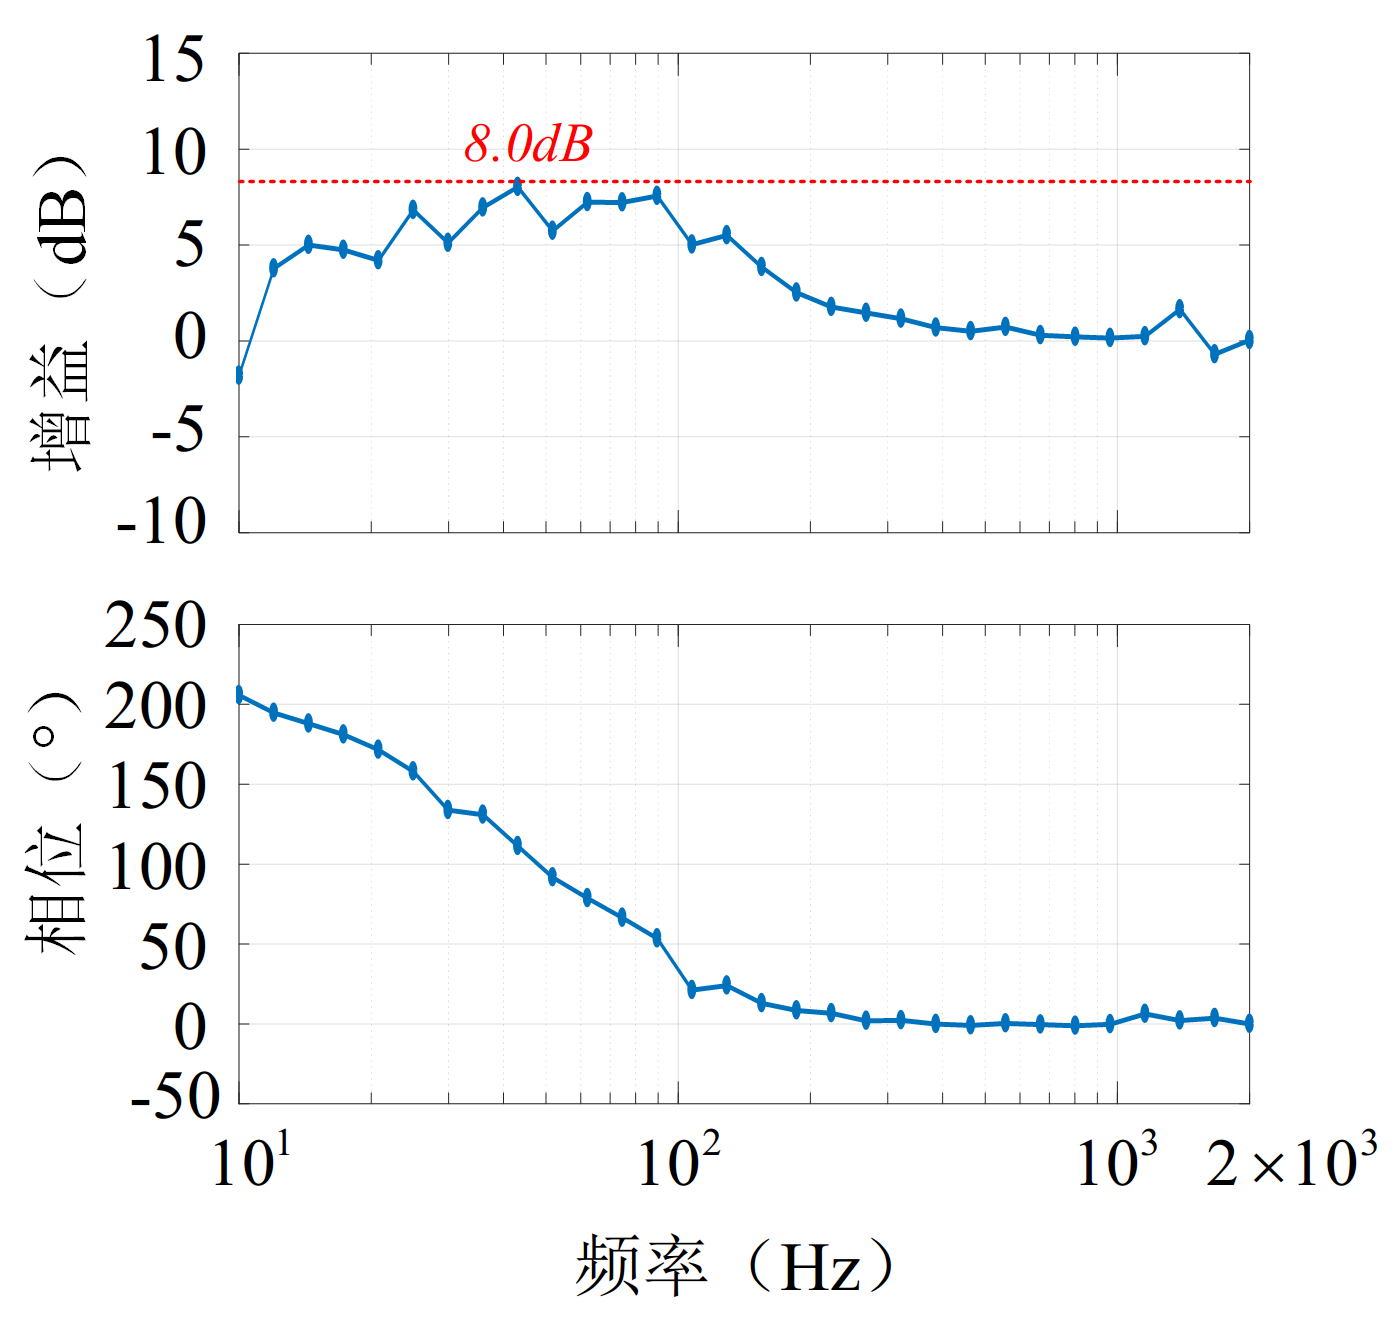
\includegraphics[scale=1.0]{5-sens_x.png}}\quad  
	\subfloat[YA控制通道输出敏感度函数曲线\label{fig:5-sens_y}]{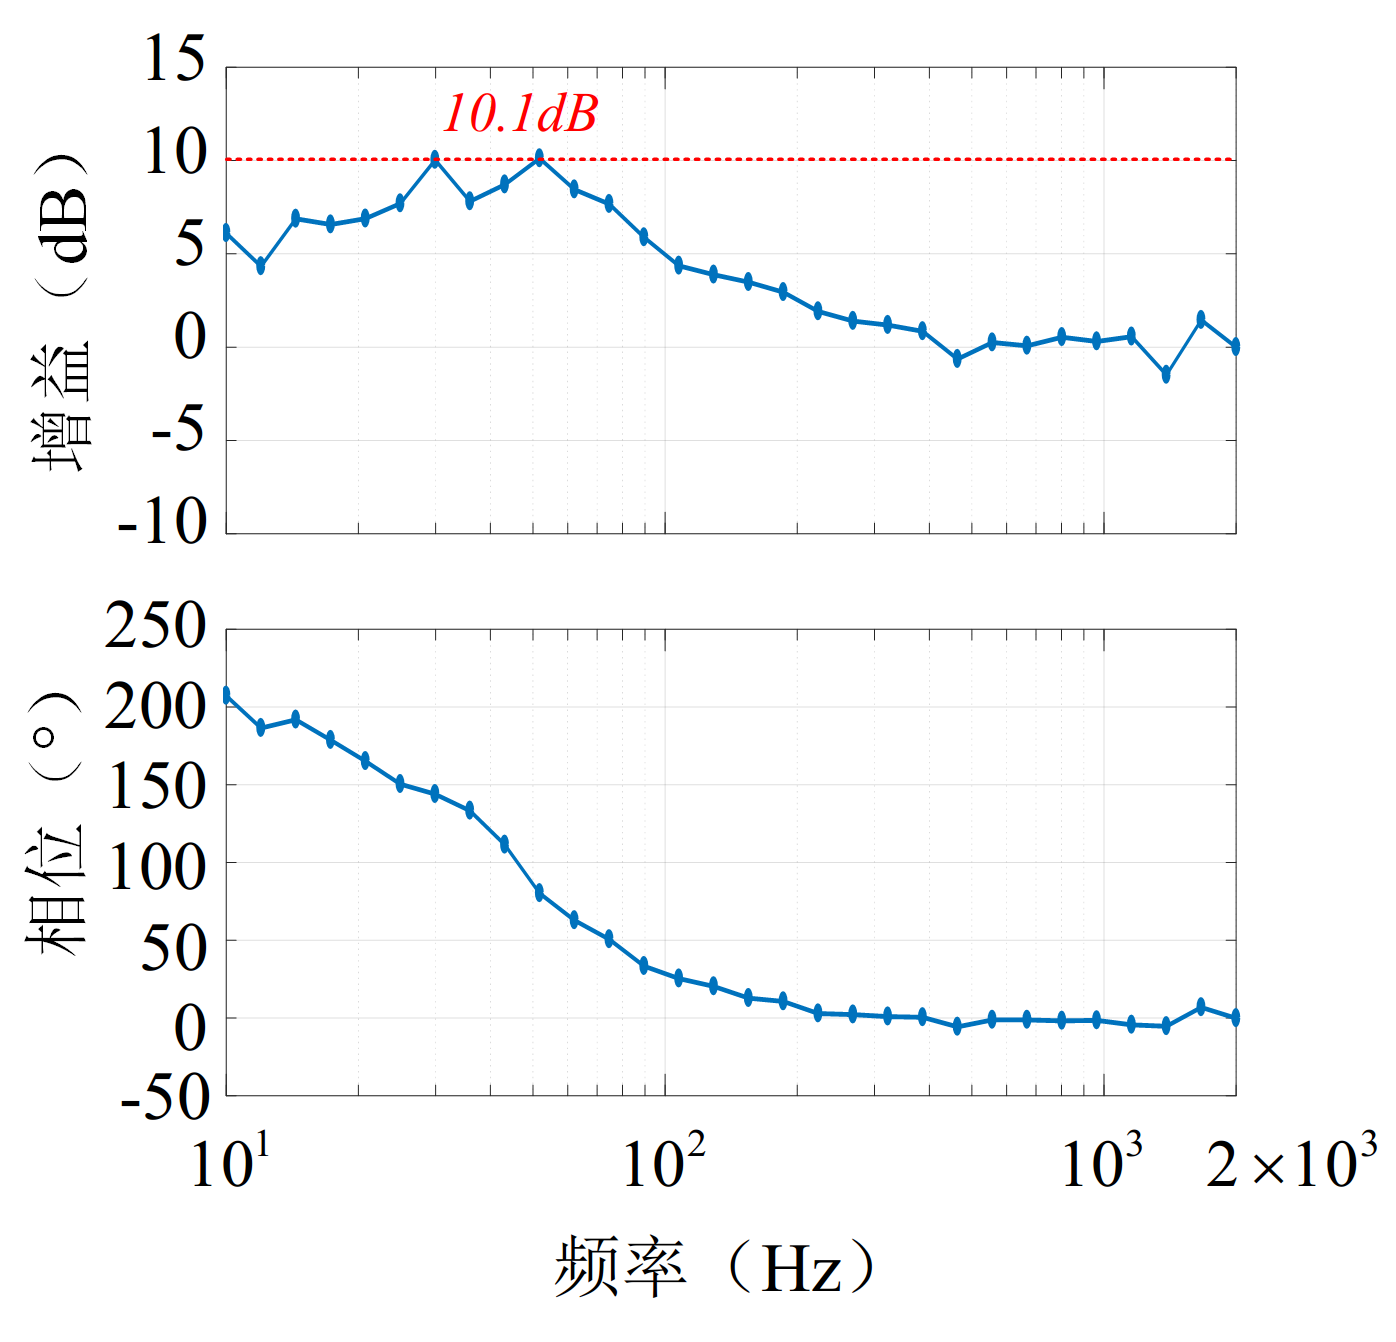
\includegraphics[scale=1.0]{5-sens_y.png}}\quad  	
	\subfloat[XB控制通道输出敏感度函数曲线\label{fig:5-sens_u}]{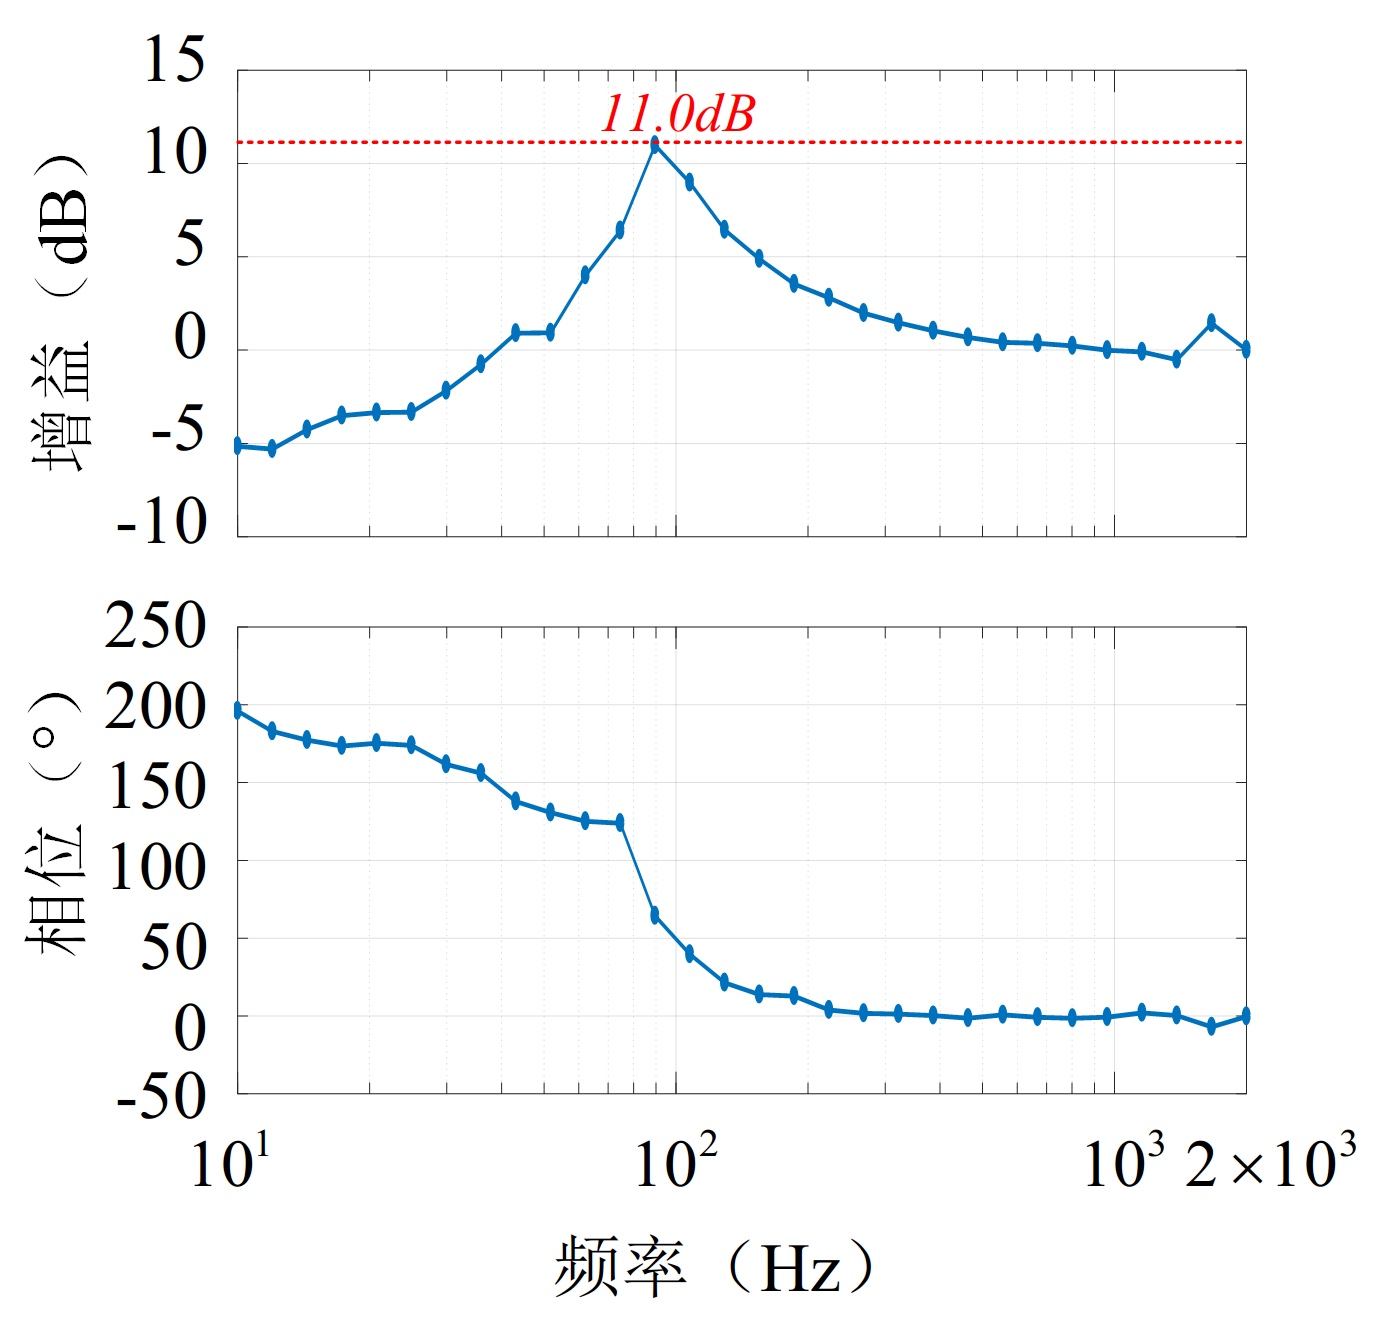
\includegraphics[scale=1.0]{5-sens_u.png}}\quad  
	\subfloat[YB控制通道输出敏感度函数曲线\label{fig:5-sens_v}]{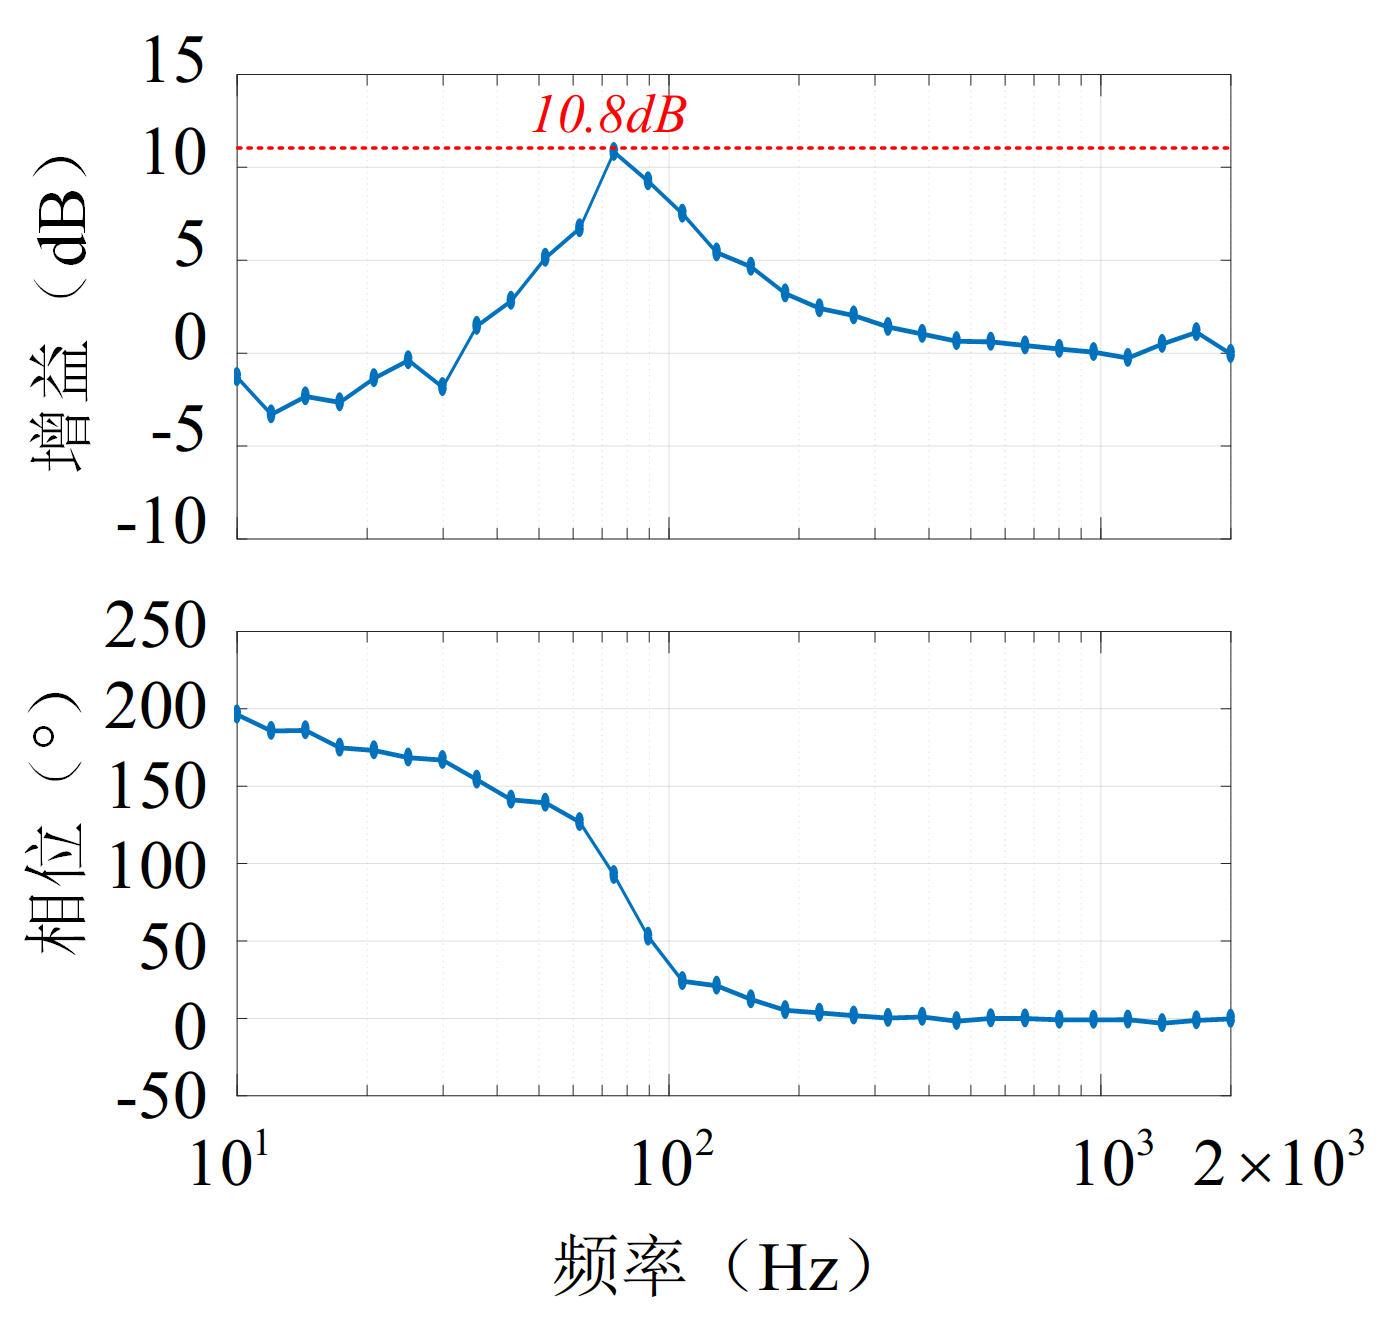
\includegraphics[scale=1.0]{5-sens_v.png}}\quad  			
	\caption{径向控制通道输出敏感度函数曲线}  \label{fig:5-sens}
\end{figure}

对于输出敏感度测量结果,ISO 14839-3定义了稳定区间标准如\autoref{tab:amb_iso}~所示。新出厂的商用磁悬浮轴承的输出敏感度峰值应落在A区间;对于非严格的使用环境,落在B区间也是可以接受的;对于输出敏感度函数峰值落在C区间的磁悬浮轴承,通常不宜长期运行;若输出敏感度函数峰值落在D区间,则表明该磁悬浮轴承应立即检修。

\begin{figure}[H]
	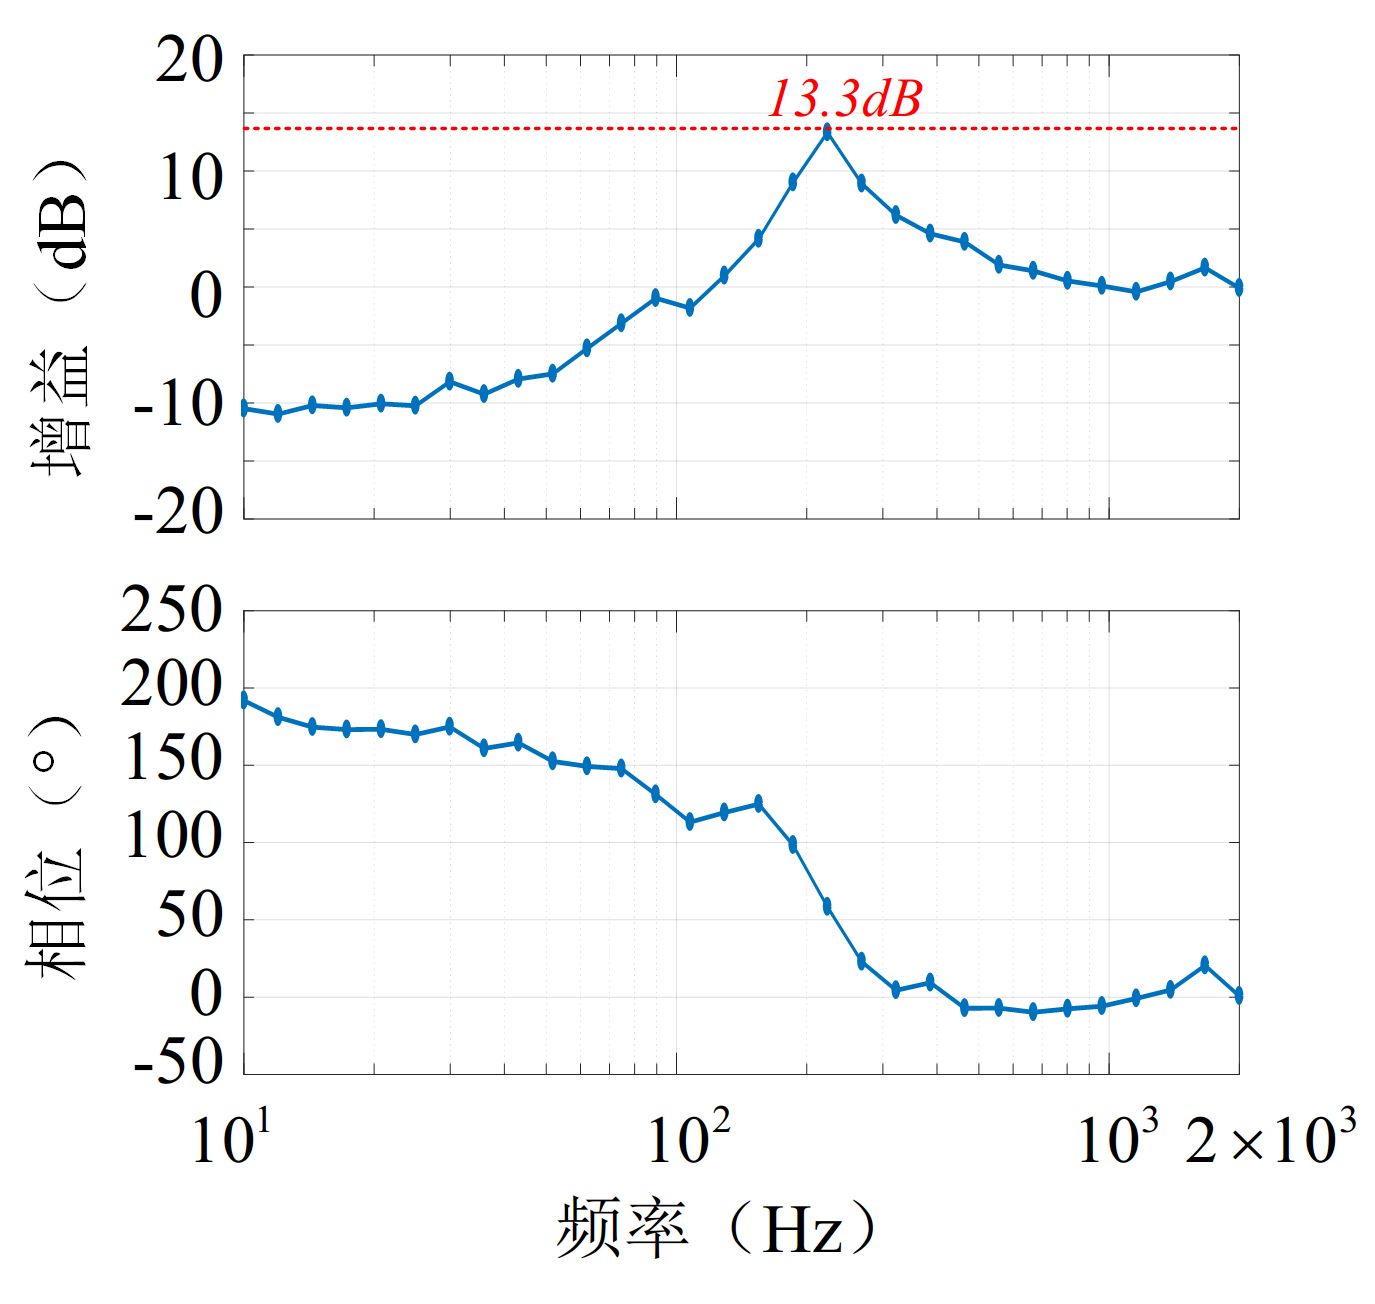
\includegraphics[scale=1.0]{5-sens_z.png}
	\caption{轴向控制通道输出敏感度函数曲线}
	\label{fig:5-sens_z}
\end{figure}

从\autoref{fig:5-sens}~和\autoref{fig:5-sens_z}~所示的输出敏感度测量结果可以看出,四个径向自由度的输出敏感度函数的峰值分别为8.0dB、10.1dB、11.0dB和10.8dB,轴向自由度的输出敏感度函数的峰值为13.3dB。其中径向自由度的输出敏感度峰值均落在B区间,轴向自由度的输出敏感度峰值落在C区间。按照ISO标准,该实验样机满足短期运转的实验测试需求。

\section{本章小结}
本节以磁悬浮离心压缩机为例,介绍了磁悬浮电机的机械结构及其控制系统组成。建立了磁悬浮轴承转子的动力学模型,以及包含质量不平衡和传感器误差因素的磁悬浮转子振动模型。本章结论如下:

(1)五自由度磁悬浮轴承转子的主动控制包含轴向平动、径向平动和转动,其中轴向运动和径向运动可视为解耦控制。

(2)质量不平衡可视为在传感器检测点引入的与转子转速同频的正弦扰动,此正弦扰动会在控制电流中引起与之同频正弦扰动电流,进而在磁轴承中产生与之同频的正弦扰动磁悬浮力。

(3)传感器误差在传感器检测点引入与转子转速成一倍或多倍关系的正弦扰动,与质量不平衡类似,最终在控制电流和磁轴承中激发谐波成分丰富的扰动成分。

(4)根据ISO磁轴承国际标准,进行了输出敏感度测定实验,实验结果显示本文研究样机悬浮性能符合实验测试需求。

\chapter{基于重复控制器的主动振动抑制方法}
本章分析重复控制器的原理,包括其组成结构、稳定性分析和应用拓扑。针对磁悬浮轴承中的同频和倍频正弦扰动,提出一种新的重复控制器算法——ZORC,以解决CRC谐波抑制频率冗余、谐波抑制效果随频率上升而削弱的问题。

\section{传统整数次重复控制器}
\subsection{工作原理}
重复控制器是基于内模原理\cite{francis1975internal}:在存在扰动信号的条件下,使闭环系统无误差地跟踪给定输入指令的一个充分条件是闭环系统中包含这个扰动信号模型。例如,在离散域下一个周期为$N$的信号可以表示为
\begin{equation}
\label{eq3-1}
W\left( z \right){\rm{ = }}{{{W_0}} \over {1 - {z^{ - N}}}}
\end{equation}
\begin{figure}[h!]
	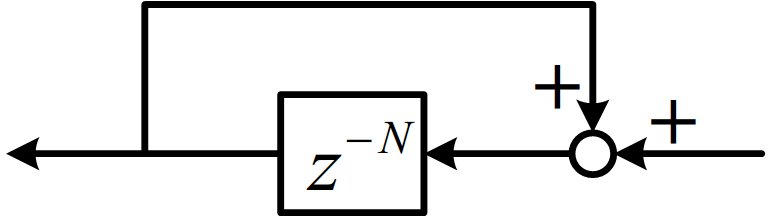
\includegraphics[scale=1.0]{3-1-generator.png}
	\caption{一种周期信号发生器}
	\label{fig:3-1-generator}
\end{figure}
其中${W_0}\left( z \right) = w\left( 0 \right) + w\left( 1 \right){z^{ - 1}} + ... + w\left( {N - 1} \right){z^{ - \left( {N - 1} \right)}}$。针对该周期信号,可以构造其对应的信号模型如\autoref{fig:3-1-generator}~所示。该环节的离散域传递函数为
\begin{equation}
\label{eq3-2}
{G_{rc}}\left( z \right){\rm{ = }}{{{z^{ - N}}} \over {1 - {z^{ - N}}}}
\end{equation}
其中$N = {{{\omega _s}} \mathord{\left/
 {\vphantom {{{\omega _s}} {{\omega _d}}}} \right.
 \kern-\nulldelimiterspace} {{\omega _d}}}$,$\omega _s$是数字控制器的采样角频率,$\omega _d$是扰动信号的基波角频率。可以看出,$G_{rc}(z)$的极点在$\omega = k\omega_d(k = 1,2,...)$处,因此对于频率为整数倍于基波频率的信号,包含该周期信号发生器的闭环回路均具有消除扰动信号、无误差跟踪给定输入指令的能力。
 
\begin{figure}[h!]
	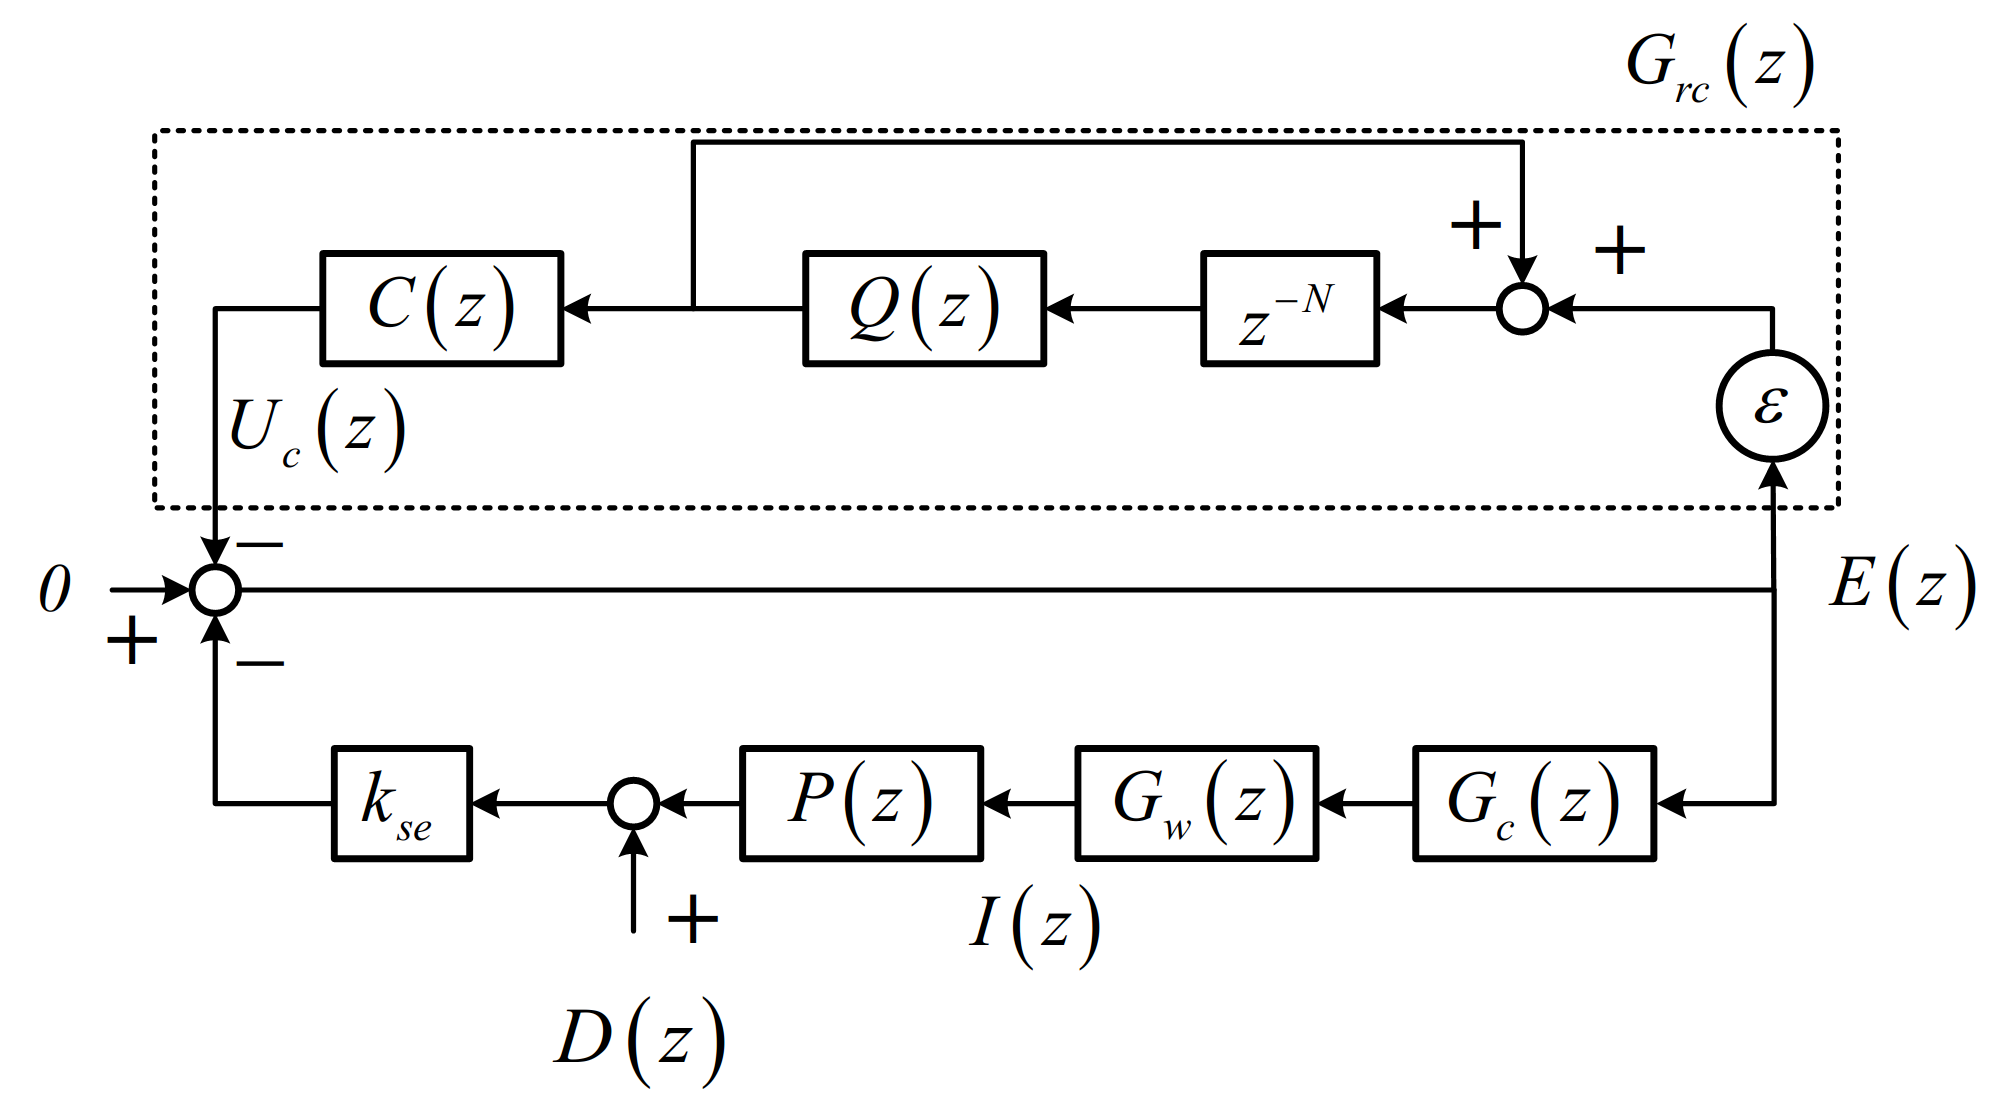
\includegraphics[scale=1.0]{3-2-crc.png}
	\caption{使用重复控制器抑制电流谐波的控制框图}
	\label{fig:3-2-crc}
\end{figure}

磁悬浮轴承位移传感器中的同频和倍频扰动信号造成控制电流中包含谐波含量丰富的振动信号,为消除振动电流以抑制振动力,通常以反馈形式插入重复控制器,应用拓扑如\autoref{fig:3-2-crc}~所示。虚线框所围区域是插入的重复控制器,其由以下部分构成:

(1)控制增益$\varepsilon $:用于调节插入式重复控制器的作用强度,该值越大,重复控制器作用强度越强,即谐波扰动信号抑制越明显。但是随着控制增益的增大,闭环回路的稳定性在随之下降。

(2)延时环节${z^{ - N}}$:用于记忆前某段时刻至当前时刻的波形,延时环节的个数与扰动信号频率、控制频率相关。

(3)低通滤波器$Q(z)$:由于实际需要被消除的周期信号中同时含有噪声等无效信号,经过延时环节的累计记忆后可能导致环路输出发散,闭环回路失稳。因此加入低通滤波器来抑制高频噪声,提升重复控制器稳定范围。

(4)相位补偿器$C(z)$:控制信号输入到重复控制器回路后,经过延时环节和低通滤波器环节后存在幅值和相位的变化,相位调节器用于调节重复控制器回路的相位,提升重复控制器的稳定范围。

位移传感器和质量不平衡引起的同频或者倍频扰动信号可以等效为位移传感器前级引入的扰动信号,将该外源扰动记为$D(z)$。将磁轴承控制电流信号记为$I(z)$,谐波抑制的目的是使$I(z)$中谐波成分降低。该插入式重复控制器的输入为位移误差信号$E(z)$,记重复控制器的输出为$U_c(z)$,那么重复控制器的计算规律可以表示为
\begin{equation}
{U_c}\left( z \right) = \frac{{\varepsilon  \cdot {z^{ - N}}Q\left( z \right)C\left( z \right)E\left( z \right)}}{{1 - {z^{ - N}}Q\left( z \right)}}
\label{eq3-3}
\end{equation}
重复控制器的开环传递函数记为$G_{rc}(z)$,其可以表示为
\begin{equation}
{G_{rc}}\left( z \right) = \frac{{{U_c}\left( z \right)}}{{E\left( z \right)}} = \frac{{{z^{ - N}}Q\left( z \right)}}{{1 - {z^{ - N}}Q\left( z \right)}}\varepsilon C\left( z \right)
\label{eq3-4}
\end{equation}
扰动信号$D(z)$到电流信号$I(z)$的传递函数记为$L_1(z)$,其可以表示为
\begin{equation}
{L_1}\left( z \right) = {L_0}\left( z \right) \cdot \frac{{1 - {z^{ - N}}Q\left( z \right)}}{{1 - {z^{ - N}}Q\left( z \right)\left[ {1 - \varepsilon \frac{{C\left( z \right){L_0}\left( z \right)}}{{{k_{se}}{G_c}\left( z \right){G_w}\left( s \right)}}} \right]}}
\label{eq3-5}
\end{equation}
其中
\begin{equation}
{L_0}\left( z \right) =  - \frac{{{k_{se}}{G_w}\left( z \right){G_c}\left( z \right)}}{{1 + {k_{se}}{G_c}\left( z \right)P\left( z \right)}}
\label{eq3-6}
\end{equation}

假设传递函数的极点在单位圆内,即闭环系统是稳定的(详细稳定性分析过程见下节)。记低通滤波器的截止频率为$\omega_c $,在$\omega<\omega_c$内,近似存在$Q(z)=1$。那么控制目标$I(z)$在与扰动信号基波频率成整数倍的频率处存在若干零点,即
\begin{equation}
\label{eq3-7}
\mathop {\lim }\limits_{\omega  \to {\omega _e}} \left\| {I\left( {j\omega } \right)} \right\| = 0
\end{equation}
其中 $\omega _e=\omega _d, 2\omega _d,...,n\omega _d$ ($n\omega _0$$<$$\omega _c$)。\autoref{eq3-7}~说明:插入重复控制器且闭环系统保持稳定的情况下,控制电流中的与转子同频以及倍频扰动信号可以被消除。
\subsection{稳定性分析}
磁悬浮轴承系统输出敏感度函数是表征磁轴承闭环系统控制性能的一个重要特征,它是指给定位移信号到位移误差信号的传递函数,可以用来衡量闭环系统的稳定性。系统输出敏感度函数的峰值越低,系统的稳定性能越好。\autoref{fig:3-2-crc}~所示的插入重复控制器的闭环系统中,加入插入式重复控制器前,系统输出敏感度函数记为$S_0(s)$,其可以表示为
\begin{equation}
{S_0}\left( z \right) = {{E\left( z \right)} \over {D\left( z \right)}}{\rm{ = }}{1 \over {1 + {G_c}\left( z \right)P\left( z \right){G_s}\left( z \right)}}
\end{equation}
扰动信号$D(z)$到电流信号$I(z)$的传递函数记为$L_0(z)$,其可以表示为
\begin{equation}
{L_0}\left( z \right) = {{I\left( z \right)} \over {D\left( z \right)}}{\rm{ = }} - {{{G_c}\left( z \right){G_s}\left( z \right)} \over {1 + {G_c}\left( z \right)P\left( z \right){G_s}\left( z \right)}}
\end{equation}
加入插入式重复控制器后,扰动信号$D(z)$到电流信号$I(z)$的传递函数记为$L_1(z)$,其可以表示为
\begin{equation}
\label{eq3-10}
\begin{aligned}
L_1(z)
&=\dfrac{I(z)}{D(z)}\\
&=\dfrac{G_c(z)G_s(z)}{1+G_c(z)P(z)G_s(z)+\dfrac{z^{-N}Q(z)}{1-z^{-N}Q(z)}\varepsilon C(z)}\\
&=\dfrac{G_c(z)G_w(z)}{1+G_c(z)P(z)G_s(z)}\cdot \dfrac{1}{1+\dfrac{z^{-N}Q(z)}{[1-z^{-N}Q(z)][1+G_c(z)P(z)G_s(z)]}\varepsilon C(z)}\\
&=\dfrac{G_c(z)G_w(z)}{1+G_c(z)P(z)G_s(z)}\cdot \dfrac{1-z^{-N}Q(z)}{1-z^{-N}Q(z)\left[1-\dfrac{1}{1+G_c(z)P(z)G_s(z)}\varepsilon C(z)\right]}\\
&=L_0(z)\dfrac{1-z^{-N}Q(z)}{1-z^{-N}Q(z)[1-\varepsilon C(z)S_0(z)]}
\end{aligned}
\end{equation}
闭环系统的稳定性充分必要条件是其在$s$域右半平面没有极点,等效于在$z$域上极点均在单位圆内。从\autoref{eq3-10}~可以看出,加入插入式重复控制器的闭环系统稳定条件是:

(1)系统输出敏感度函数$S_0(z)$的极点在单位圆内;

(2)$\left\| Q(z)[1 - \varepsilon C(z)S_0(z)] \right\| < 1$

通常在加入插入式重复控制器之前,通过设计合适的控制器$G_c(z)$的参数来使闭环系统稳定。因此条件1通常在加入插入式重复控制器之前得到满足。通过设计合适的重复控制器参数,包括$\varepsilon$、$Q(z)$、$C(z)$来使加入插入式重复控制器的系统保持稳定。
\section{零相移奇数次重复控制器}
磁悬浮轴承中谐波扰动信号通常是奇数倍于基波频率,使用CRC可以消除所有奇数次谐波扰动,但是其在偶数谐波出的抑制作用是冗余的。如果重复控制器可以仅在奇数次频率处起作用,那么加入的插入式重复控制器可以避免对偶数次频率处的系统特性产生影响。此外,为了维持闭环系统的稳定性,重复控制器环路中的低通滤波器是必不可少的组成成分。然而低通滤波器对有效信号的幅值衰减和相位偏移特性将会导致重复控制器谐波抑制作用减弱。

针对CRC的在磁轴承中应用的弊端,本节提出ZORC,其改进点在于:

(1)将CRC中的整数次周期信号发生器改为奇数次周期信号发生器,使得重复控制器仅消除奇数次谐波;

(2)将低通滤波器从重复控制器延时环路内移动到延时环路外,保证闭环系统稳定性的同时,可以有效提高重复控制器谐波抑制能力;

(3)将传统的一阶低通滤波器改为零相移低通滤波器,保留其对信号幅值衰减特性的能力,同时避免对信号的相位偏移。

\subsection{工作原理}
对于\autoref{eq3-2}~所表示的周期信号模型,其可以分解表示为
\begin{equation}
G_{rc}(z)=\dfrac{1}{2}\left(\dfrac{1}{1-z^{-N/2}}-\dfrac{1}{1+z^{-N/2}}\right)
\end{equation}
代入$N=\dfrac{\omega_s}{\omega_d}$、$z=e^{j\omega T_s}$其中$T_s$是采样周期。那么上式可以表示为
\begin{equation}
G_{rc}(j\omega)=\frac{1}{2}\left(\frac{1}{1-e^{-j\pi\frac{\omega}{\omega_D}}}-\frac{1}{1+e^{-j\pi\frac{\omega}{\omega_D}}}\right)
\end{equation}
对于${1}/\left(1-e^{-j\pi\frac{\omega}{\omega_d}}\right)$,其极点在$\omega=2k\omega_d$处$(k=0,1,2,..)$,该项可以消除频率是偶数倍于基波频率的扰动信号;对于${1}/\left(1+e^{-j\pi\frac{\omega}{\omega_d}}\right)$,其极点在$\omega=(2k-1)\omega_d$处$(k=0,1,2,..)$,该项可以消除频率是奇数倍于基波频率的扰动信号。

若将\autoref{eq3-2}~所表示的周期信号模型称之为整数次周期信号发生器,那么由上述推导可见,其可以分解成为奇数次信号发生器和偶数次信号发生器,如\autoref{fig:3-3-odd_generator}~所示。仅取其奇数次周期信号发生器部分,替换CRC中的整数次周期信号发生器部分,即构成奇数次重复控制器。
\begin{figure}
	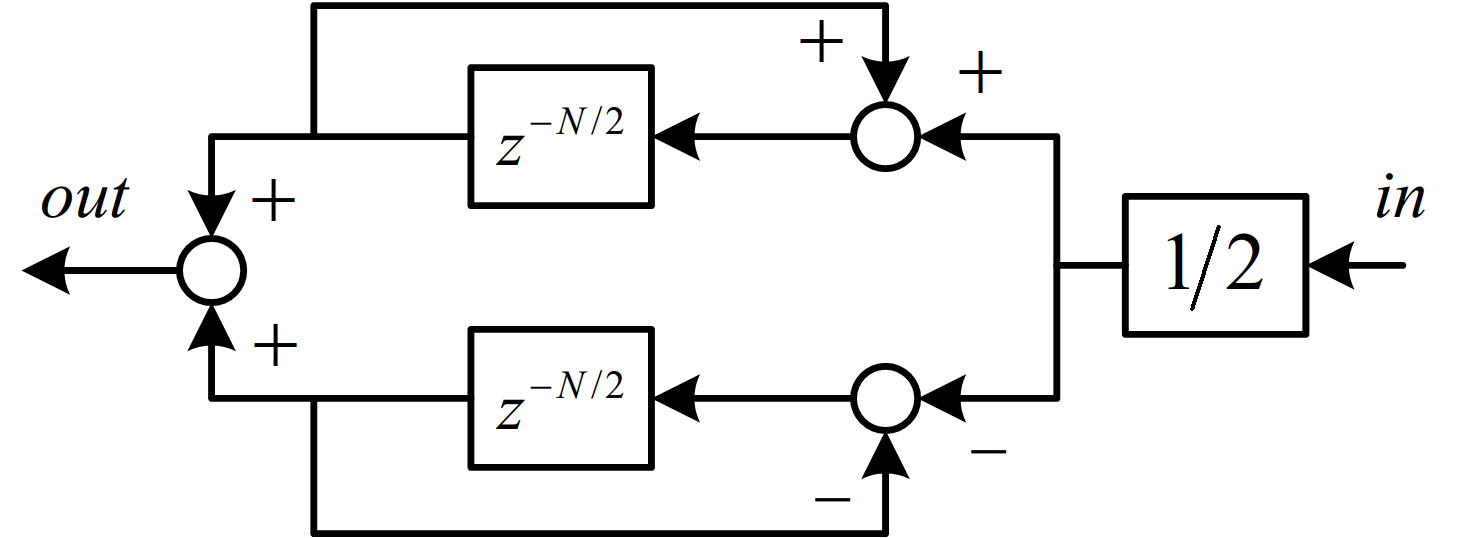
\includegraphics[scale=1.0]{3-3-odd_generator.png}
	\caption{奇数次、偶数次信号发生器组合示意图}
	\label{fig:3-3-odd_generator}
\end{figure}
加入奇数次重复控制器的磁轴承系统控制框图如\autoref{fig:orc}~所示。
\begin{figure}[h!]
	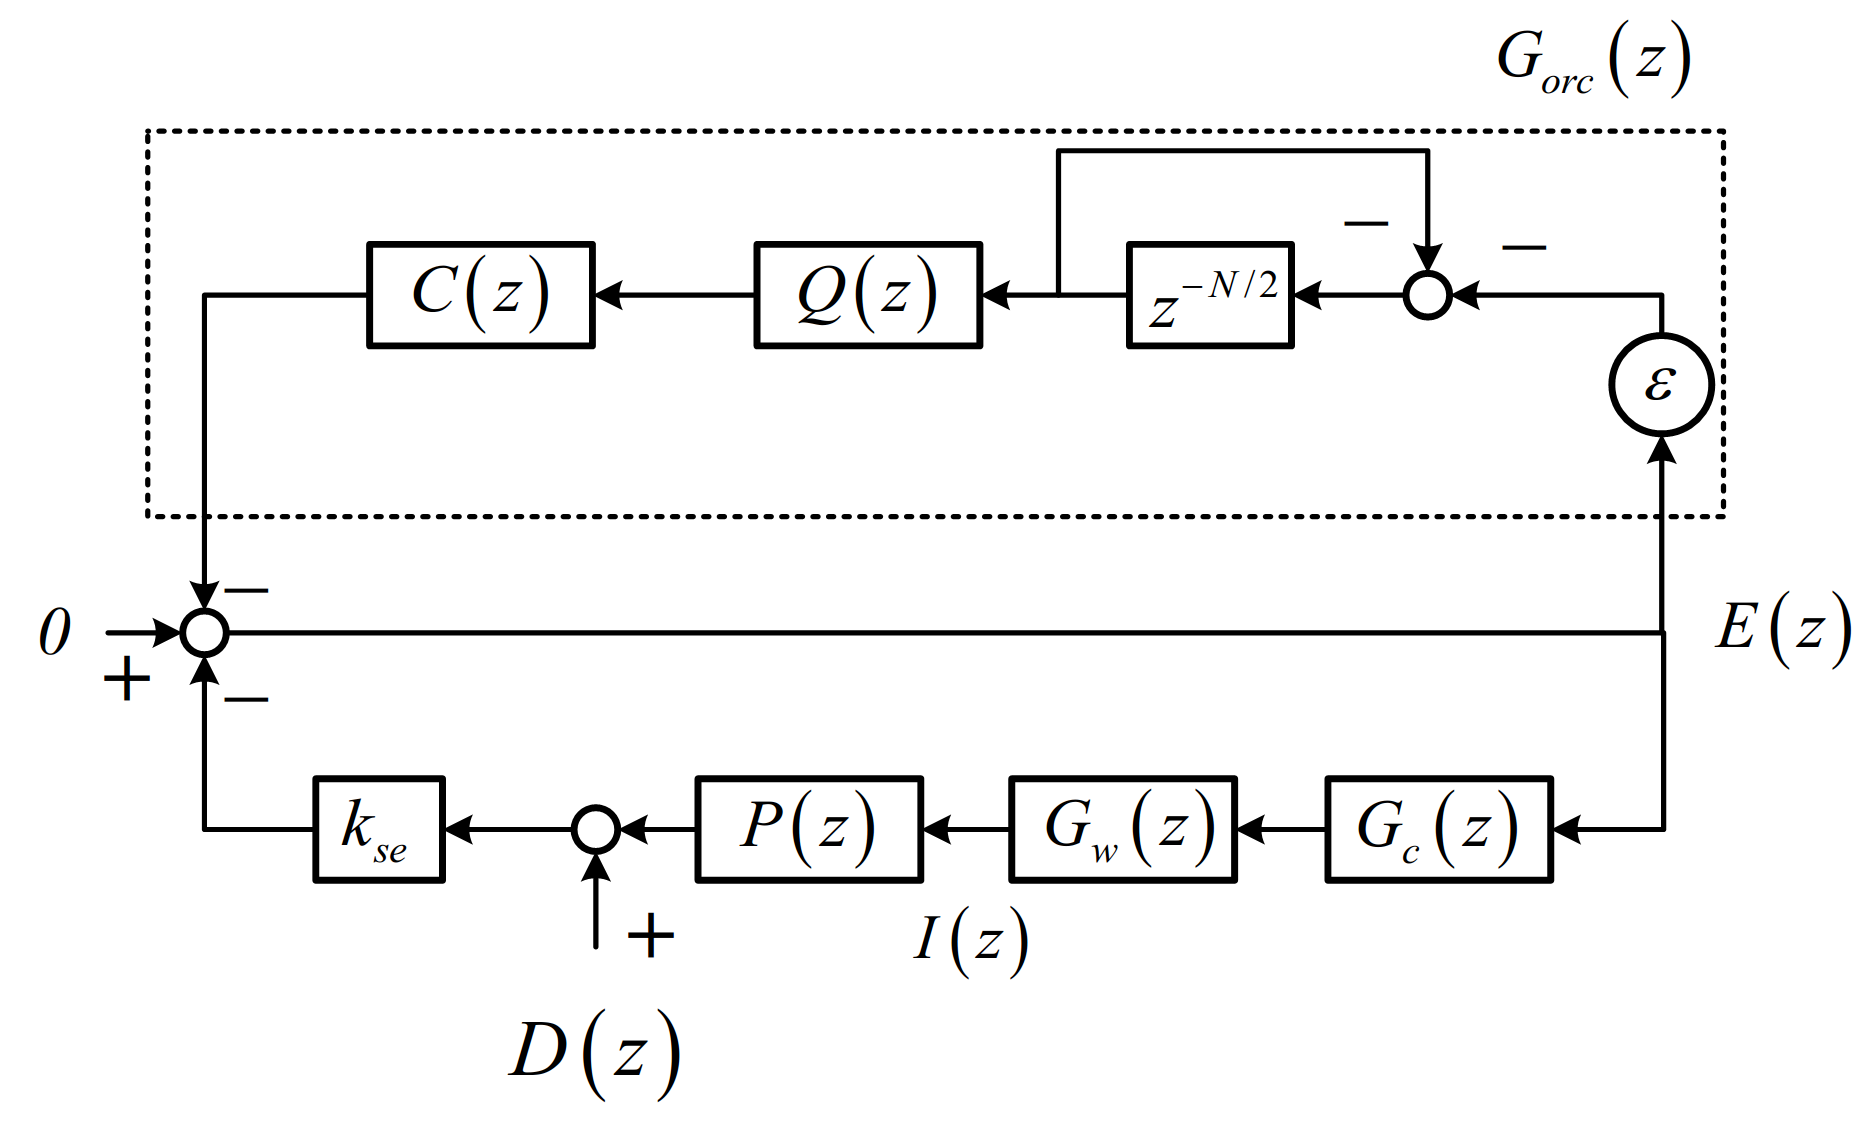
\includegraphics[scale=1.0]{3-4-orc.png}
	\caption{使用奇数次重复控制器抑制电流谐波的控制框图}
	\label{fig:orc}
\end{figure}
奇数次重复控制器的开环传递函数记为$G_{orc}(z)$,其可以表示为
\begin{equation}
G_{orc}(z)=\dfrac{z^{-N}}{1-z^{-N}Q(z)}\varepsilon C(z)
\end{equation}
记扰动信号$D(z)$到控制电流信号$I(z)$的传递函数为$L_2(z)$,其可以表示为
\begin{equation}
L_1(z)={L_0}\left( z \right) \cdot {{1 + {z^{ - N/2}}} \over {1 - {z^{ - N/2}}\left[ {\varepsilon Q\left( z \right)C\left( z \right){S_0}\left( z \right) - 1} \right]}}
\end{equation}
假设传递函数的极点在单位圆内,即闭环系统是稳定的(详细稳定性分析过程见下节)。那么控制目标$I(z)$在与扰动信号基波频率成奇数倍的频率处存在若干零点,即
\begin{equation}
\label{eq3-10_1}
\mathop {\lim }\limits_{\omega  \to {\omega _e}} \left\| {I\left( {j\omega } \right)} \right\| = 0
\end{equation}
其中 $\omega _e=\omega _d, 3\omega _d,...,(2k-1)\omega _d$。\autoref{eq3-10_1}~说明:加入奇数次重复控制器且闭环系统保持稳定的情况下,控制电流中的与转子同频以及奇数倍频扰动信号可以被消除。
\subsection{稳定性分析}
加入重复控制器后,扰动信号$D(z)$到电流信号$I(z)$的传递函数记为$L_2(z)$,其可以表示为
\begin{equation}
\label{eq3-11}
\begin{aligned}
L_2(z)
&=\dfrac{I(z)}{D(z)}\\
&=\dfrac{G_c(z)G_s(z)}{1+G_c(z)P(z)G_s(z)+\dfrac{z^{-N}}{1-z^{-N}Q(z)}\varepsilon C(z)}\\
&=\dfrac{G_c(z)G_w(z)}{1+G_c(z)P(z)G_s(z)}\cdot \dfrac{1-z^{-N}}{1-z^{-N}Q(z)\left[1-\dfrac{1}{1+G_c(z)P(z)G_s(z)}\varepsilon C(z)\right]}\\
&=L_0(z)\dfrac{1-z^{-N}}{1-z^{-N}Q(z)[1-\varepsilon C(z)S_0(z)]}
\end{aligned}
\end{equation}
闭环系统的稳定性充分必要条件是其在$s$域右半平面没有极点,等效于在$z$域上极点均在单位圆内。从\autoref{eq3-11}~可以看出,加入重复控制器的闭环系统稳定条件是:

(1)系统输出敏感度函数$S_0(z)$的极点在单位圆内;

(2) 

	\begin{equation}
		\label{eq_stable_odd}
		\left\|1 - \varepsilon C(z)S_0(z) \right\| < 1
	\end{equation}
	
与应用CRC类似,通常在加入重复控制器之前,通过设计合适的控制器$G_c(z)$的参数来使闭环系统稳定。因此条件1通常在加入重复控制器之前得到满足。通过设计合适的重复控制器参数,包括$\varepsilon$、$Q(z)$、$C(z)$来使加入零相移奇数次重复控制器的系统保持稳定。
\subsection{零相移低通滤波器设计}
在设计参数控制增益$\varepsilon$和相位调节器$C(z)$之前,需要分析低通滤波器$Q(z)$的参数特性。低通滤波器用于提升重复控制器的稳定范围,理想的低通滤波器是在截止频率前的增益衰减比例为1,截止频率之后频率-增益曲线下降斜率大。传统整数次重复控制器中采用一阶低通滤波器,其形式为:
\begin{equation}
Q(s)=\dfrac{1}{\dfrac{s}{2\pi\cdot f_c}+1}
\end{equation}
该形式的低通滤波器具有形式简单、阶数低的优点,但是其截止频率处的下降斜率并不足够大。此外,该低通滤波器将引入相位延迟,降低重复控制器对谐波的抑制能力。为克服以上弊端,一种更优的消除低频扰动信号的方案是使用零相移低通滤波器。

零相移低通滤波器是一种非因果滤波器,其当前时刻的输出取决于当前时刻的输入和下一时刻的输入。在常规的线性系统中,非因果滤波器无法实现,因为滤波器无法预知下一时刻的输入信号;而在重复控制器环路中,由于若干延时单元的存在,对于其中的非因果滤波器来说,其下一时刻的输入是预先知道的。因此在重复控制器的环路中,非因果滤波器是可以在数字控制器中部署并执行的。

本文采用的非因果低通滤波器形式如下
\begin{equation}
\label{eq3-18}
Q(z)=az+b+az^{-1}
\end{equation}
其中$a$和$b$是待设计的滤波器参数。带入$z=e^{j\omega T_s}$到\autoref{eq3-18}~中,将该式重写为:
\begin{equation}
\label{eq3-19}
Q(j\omega)=ae^{j\omega T_s}+b+ae^{-j\omega T_s}
\end{equation}
对\autoref{eq3-19}~使用欧拉公式得到:
\begin{equation}
\label{eq3-20}
Q(j\omega)=2a\cdot cos(\omega T_s)+b
\end{equation}
从\autoref{eq3-20}~可以看出$Q(j\omega)$没有虚部,因此在重复控制器环路中,该低通滤波器不会引入相位偏移。为了在低通滤波器截止频率前得到单调下降的的幅频曲线,参数$a$和$b$需要满足以下条件:
\begin{equation}
\label{eq3-21}
2a<b
\end{equation}
为了寻找一组较优的$Q(z)$参数,研究不同参数下的幅频曲线。以工作转速为250Hz为例,此工况下系统中的主要谐波成分为250Hz、750hz、1250Hz和1750Hz,欲消除七次及以下谐波,则低通滤波器的截止频率应该略高于1750Hz,此处取2250Hz。
\begin{figure}[h!]
	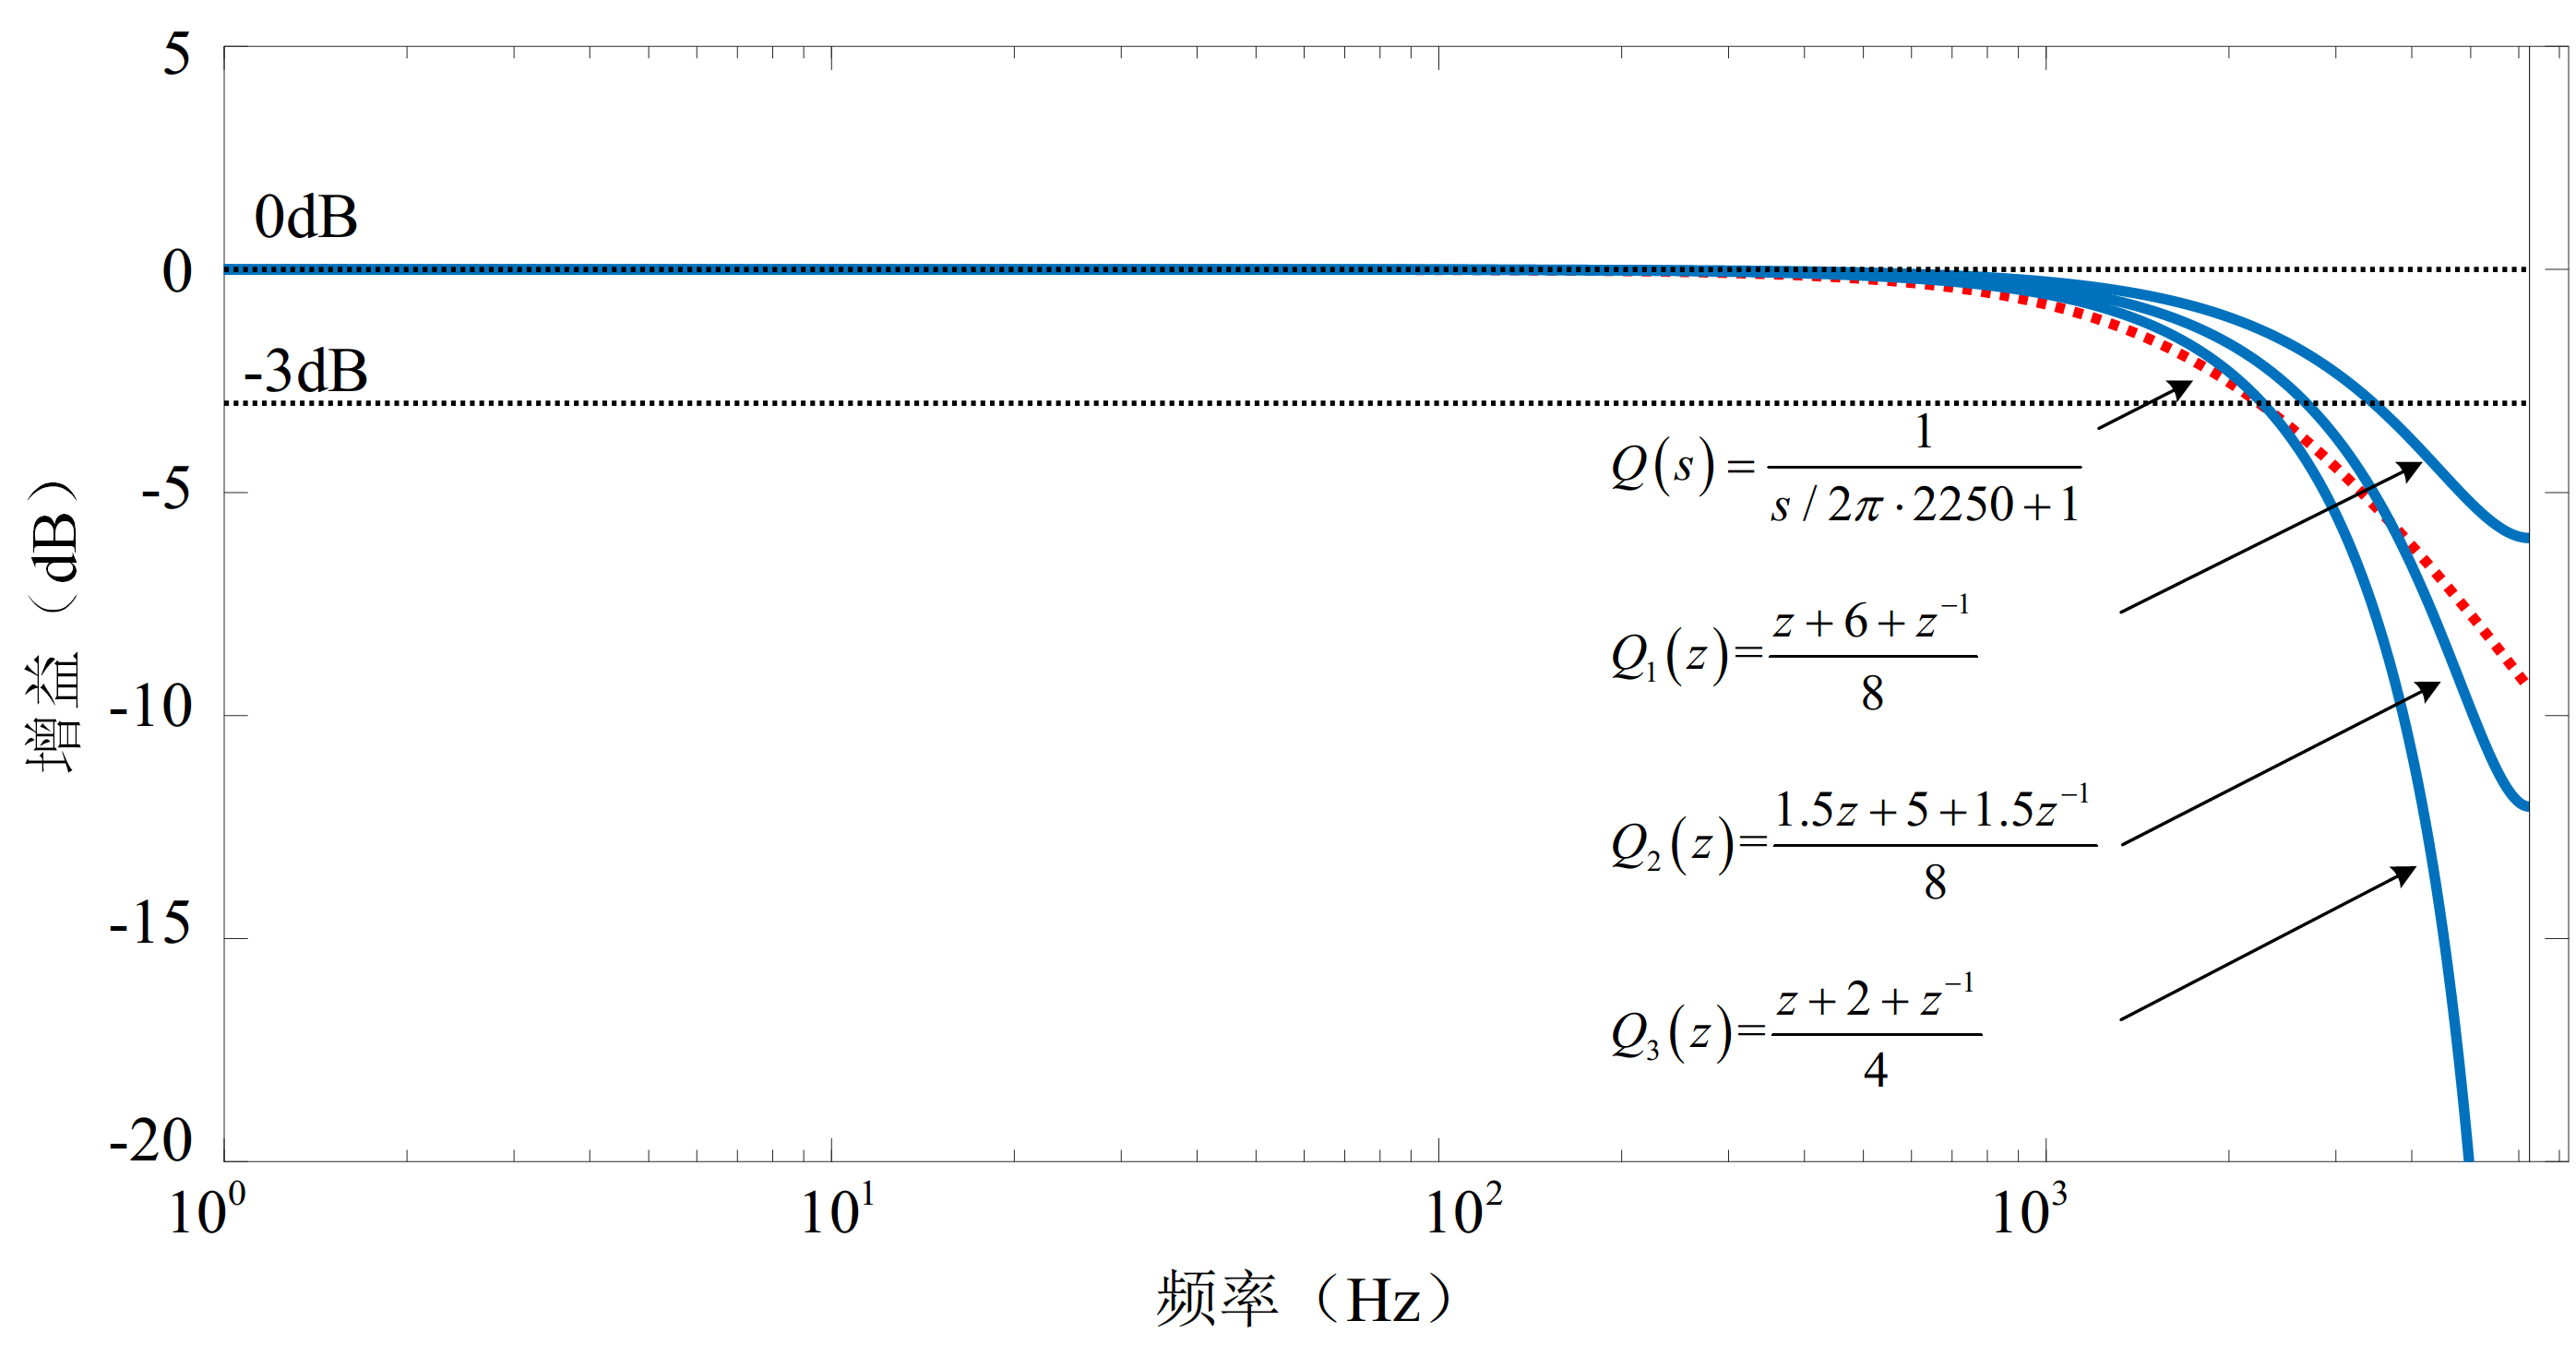
\includegraphics[scale=1.0]{3-5-lpf.png}
	\caption{不同参数下的低通滤波器幅频曲线}
	\label{fig:3-5-lpf}
\end{figure}

从\autoref{fig:3-5-lpf}~可见,与一阶低通滤波器$Q(s)$相比,$Q_3(z)$在低频处的增益更接近0dB,同时在截止频率之后的斜率更大,因此$Q_3(z)$比$Q(s)$使得重复控制器有更好的稳态性能和稳定范围。同时,可以看到随着参数$b$的值增大,$Q(z)$在截止频率处的斜率逐渐减小。因此,最终选择参数为$a=1/4$,$b=1/2$。
\subsection{相位补偿器设计}
当闭环系统稳定时,控制增益$\varepsilon$越大,误差收敛速度越快,同时插入式重复控制器环路对谐波信号的抑制能力越强。设计相位补偿器$C(z)$的目的是保证控制增益$\varepsilon$取值较大的同时,系统仍然稳定。

将磁轴承系统输出敏感度函数重写为
\begin{equation}
\label{eq_s0z}
S_0(z)=\frac{1}{1+G_w(z)G_c(z)P(z)G_s(z)}=\frac{z^{-d}B(z)}{A(z)}
\end{equation}
其中$d$表示数字控制系统中已知的延时拍数。加入插入式控制控制器之前,闭环系统已经稳定,因此$A(z)$的根均在单位圆内。假设$B(z)$与$1+z^{-\frac{N}{2}}$互质,即$B(e^{-jn\pi})B(e^{jn\pi})\neq 0$($n=1,3,5,...$),该假设是控制电流$L_2(k)$收敛的必要条件。

将$B(z)$因式分解为
\begin{equation}
B(z)=B^-(z)B^+(z)
\end{equation}
其中$B^-(z)$和$B^+(z)$分别是$B(z)$的可消除部分和不可消除部分:$B^-(z)$包含了$B(z)$在单位圆外以及不想被消除的根,$B^+(z)$是$B(z)$所有的根除掉$B^-(z)$部分的根后剩下的根。

针对\autoref{eq_s0z}~所代表的闭环系统,相位补偿器$C(z)$通常设计为
\begin{equation}
\label{eq_c(z)}
C(z)=\frac{z^{-n_u}A(z)B^-(z^{-1})}{B^+(z)b}
\end{equation}
其中,

(1)$n_u$是$B^-(z)$的阶数,此项是使得相位补偿器可实现的必不可少的成分;

(2)$B^-(z^{-1})$是通道将$B^-(z)$中的$z$用$z^{-1}$替换得到的;

(3)如果$B^-(z)$的根均在$z$域左半平面,则取$b={\left[ B^-(1)\right]}^2$;如果$B^-(z)$的根均在$z$域右半平面,则取$b={\left[ B^-(-1)\right]}^2$。

结合\autoref{eq_s0z}~和\autoref{eq_c(z)}~,\autoref{eq_stable_odd}~所示的稳定性条件可以重写为
\begin{equation}
	\label{eq_stable_odd_simplified}
	\left\|\varepsilon Q(z)\frac{B^-(z)B^-(z^{-1})}{b}-1\right\|<1
\end{equation}
因此,通过\autoref{eq_stable_odd_simplified}~可以得到控制增益$\varepsilon$的取值范围是
\begin{equation}
	\label{eq_range_gain}
	0 < \varepsilon < \frac{2}{max\left \| \frac{B^-(z)B^-(z^{-1})}{b}\right \|Q(z)}
\end{equation}

在实际应用中,定义重构谱为$R(z)$:
\begin{equation}
	\label{eq_Rz}
	R(z)=\varepsilon Q(z)S_0(z)	- 1
\end{equation}
如果$R(z)$的峰值小于1,那么为了简化相位补偿器和算法部署流程,可以取$C(z)=1$。因为此条件下\autoref{eq_stable_odd}~所表示的系统稳定的充分条件已经满足。控制增益$\varepsilon$可以依据\autoref{eq_range_gain}~进行设计,但是注意到当控制增益$\varepsilon$等于$0$时,重复控制器环路不起作用。因此在实际部署算法时,可以从$0$开始逐渐增大控制控制增益$\varepsilon$的取值,根据实际系统的电流或位移波形来调节控制增益$\varepsilon$的大小。
\section{仿真与实验分析}

该磁悬浮空气压缩机的额定转速是833Hz,其转子在闭环控制下的共振频率在低频段,即转速越低,转子振动越剧烈。因此,选取低频段频率作为ZORC性能测试频率。本文仿真和实验部分测试重复控制器对基波频率为250Hz的扰动信号的抑制能力。
\begin{figure}[h!]
	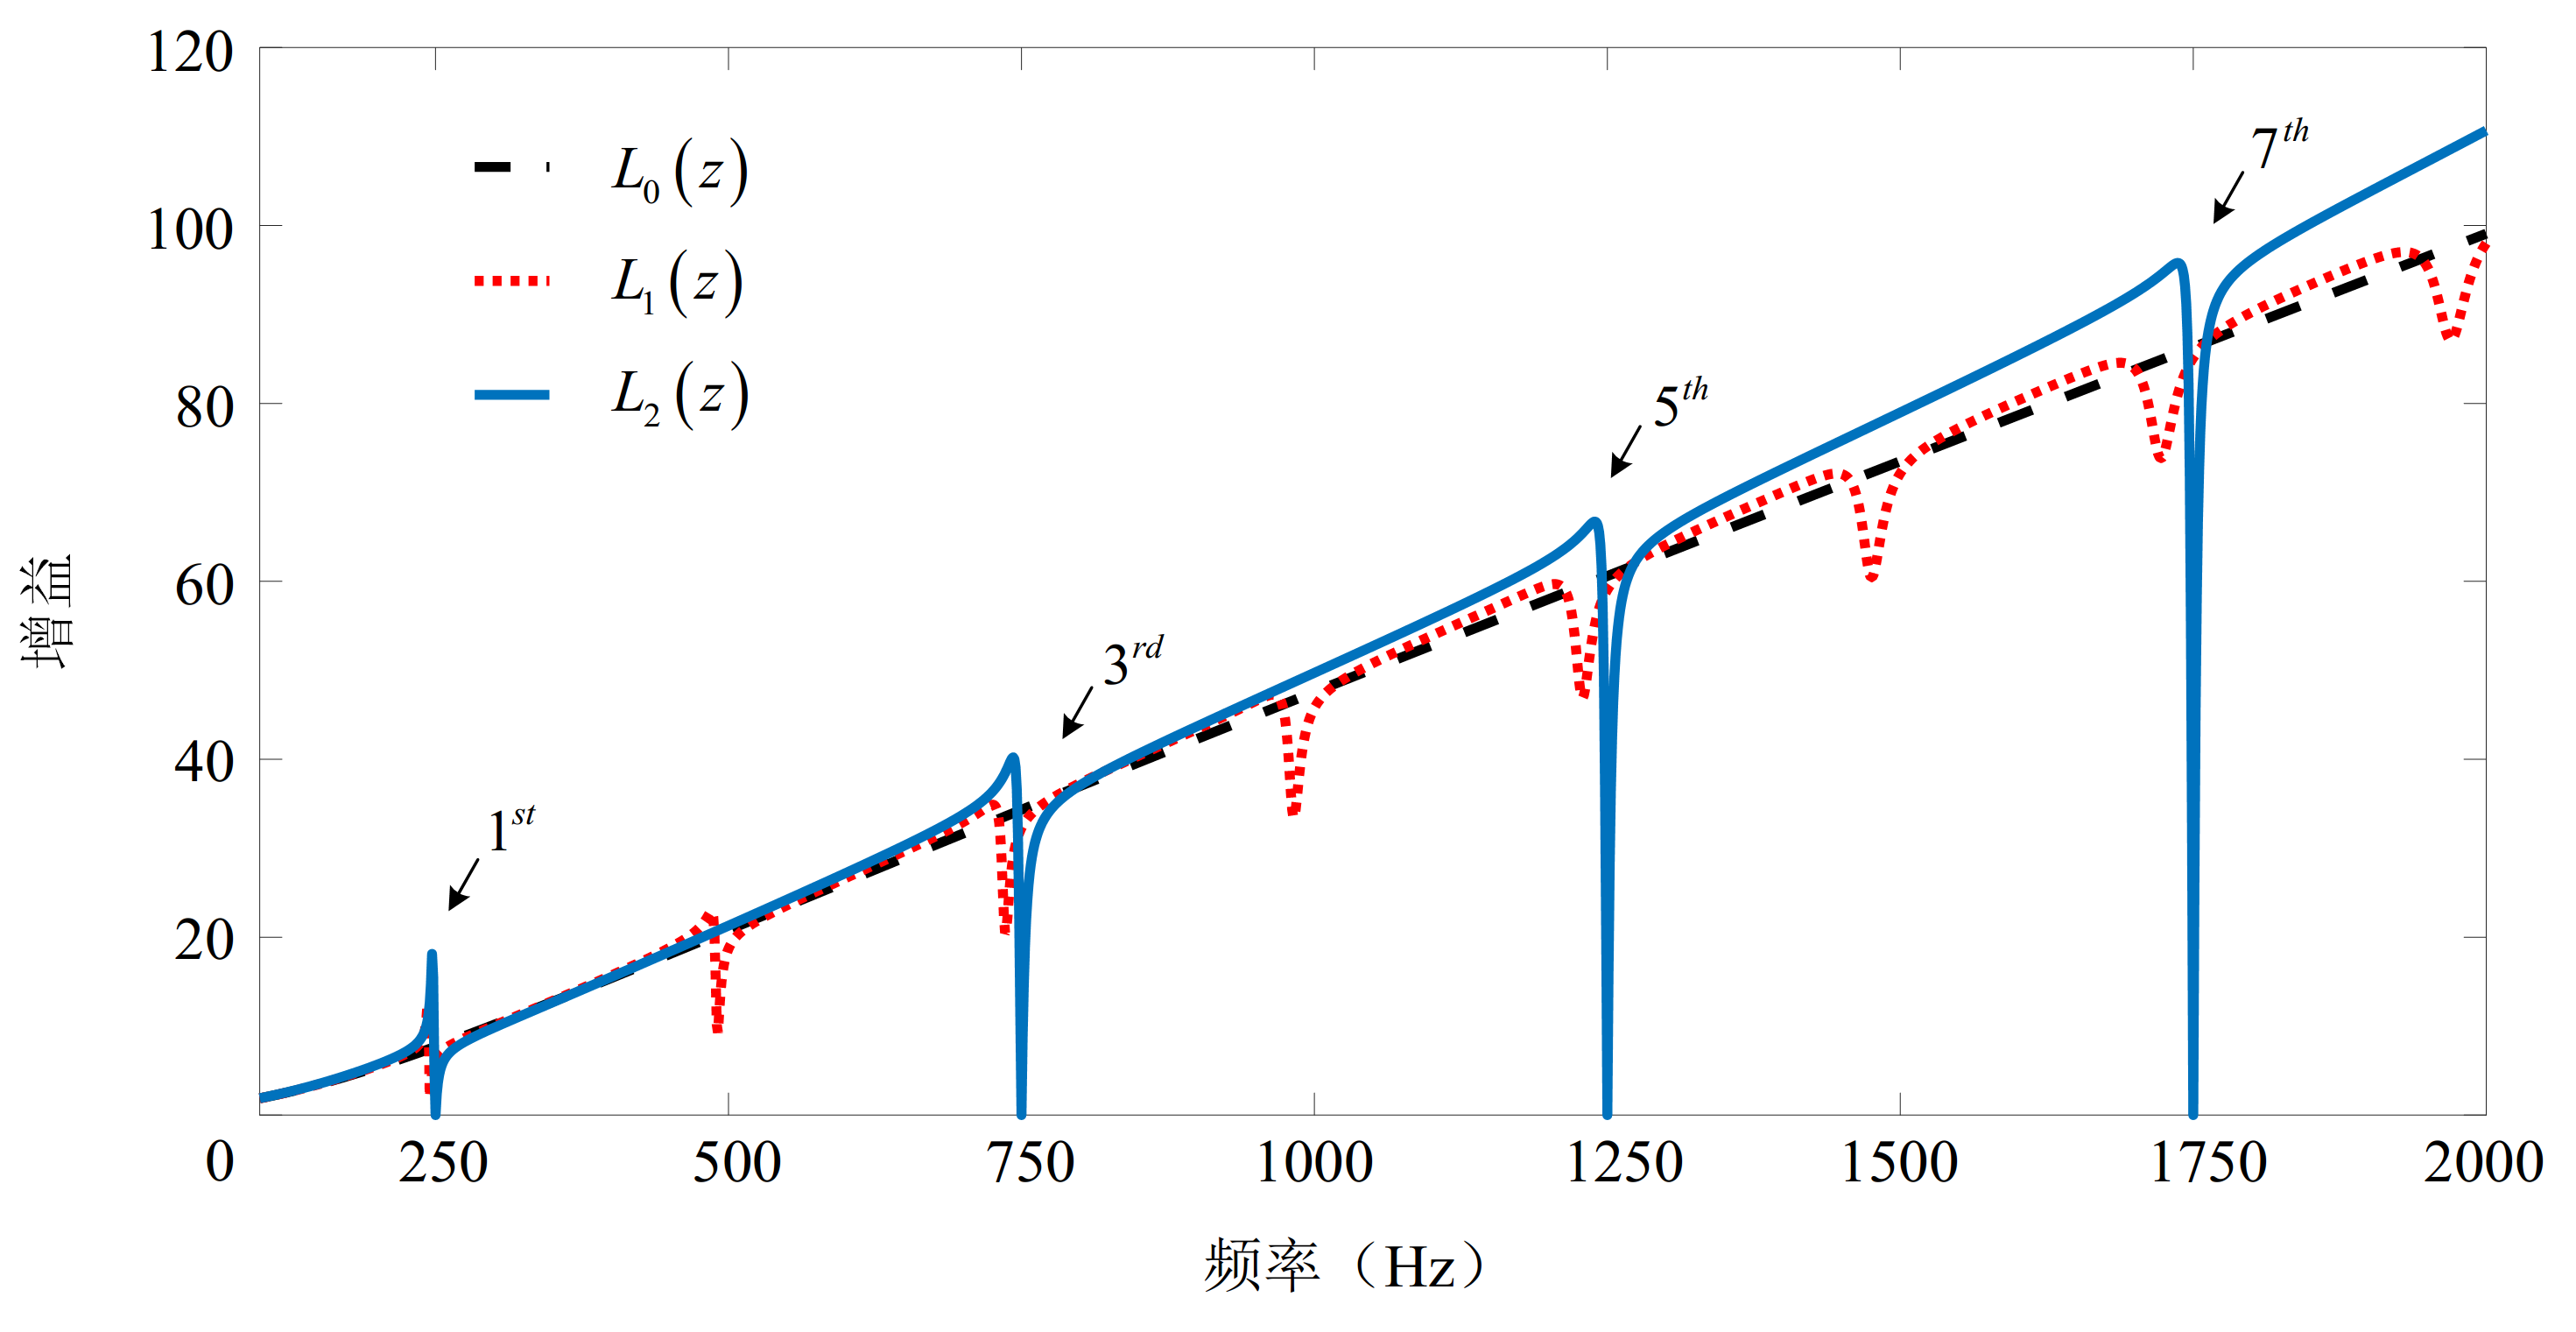
\includegraphics[scale=1.0]{3-sensitivity.png}
	\caption{$L_0(z)$、$L_1(z)$和$L_2(z)$传递函数幅频曲线}
	\label{fig:3-sensitivity}
\end{figure}

\autoref{fig:3-sensitivity}~显示了$L_0(z)$、$L_1(z)$和$L_2(z)$传递函数幅频曲线。可以看到,除了凹陷处有差异,$L_0(z)$、$L_1(z)$和$L_2(z)$曲线形状基本一致,表明插入重复控制器并不改变电流传递函数在凹陷频率之外的特性。$L_0(z)$是一个平滑的曲线,因此不插入重复控制器的闭环系统不具备抑制谐波电流的能力。$L_1(z)$和$L_2(z)$在陷波频率处有一定程度的凹陷,因此CRC和ZORC均可以抑制谐波电流。然而从图中可以看出,随着频率升高,整数次重复控制器的陷波频率逐渐发生偏移250Hz、500Hz、750Hz,…,这使得其谐波抑制能力逐渐下降。此外,其偶数倍于基波频率的陷波频率是没有必要的。与之相对比的是$L_2(z)$的陷波频率均准确定在奇数倍与基波频率处,没有发生偏移,且曲线凹陷程度比$L_1(z)$更深。这使得ZORC拥有更优的谐波抑制能力。

\begin{figure}[h!]
	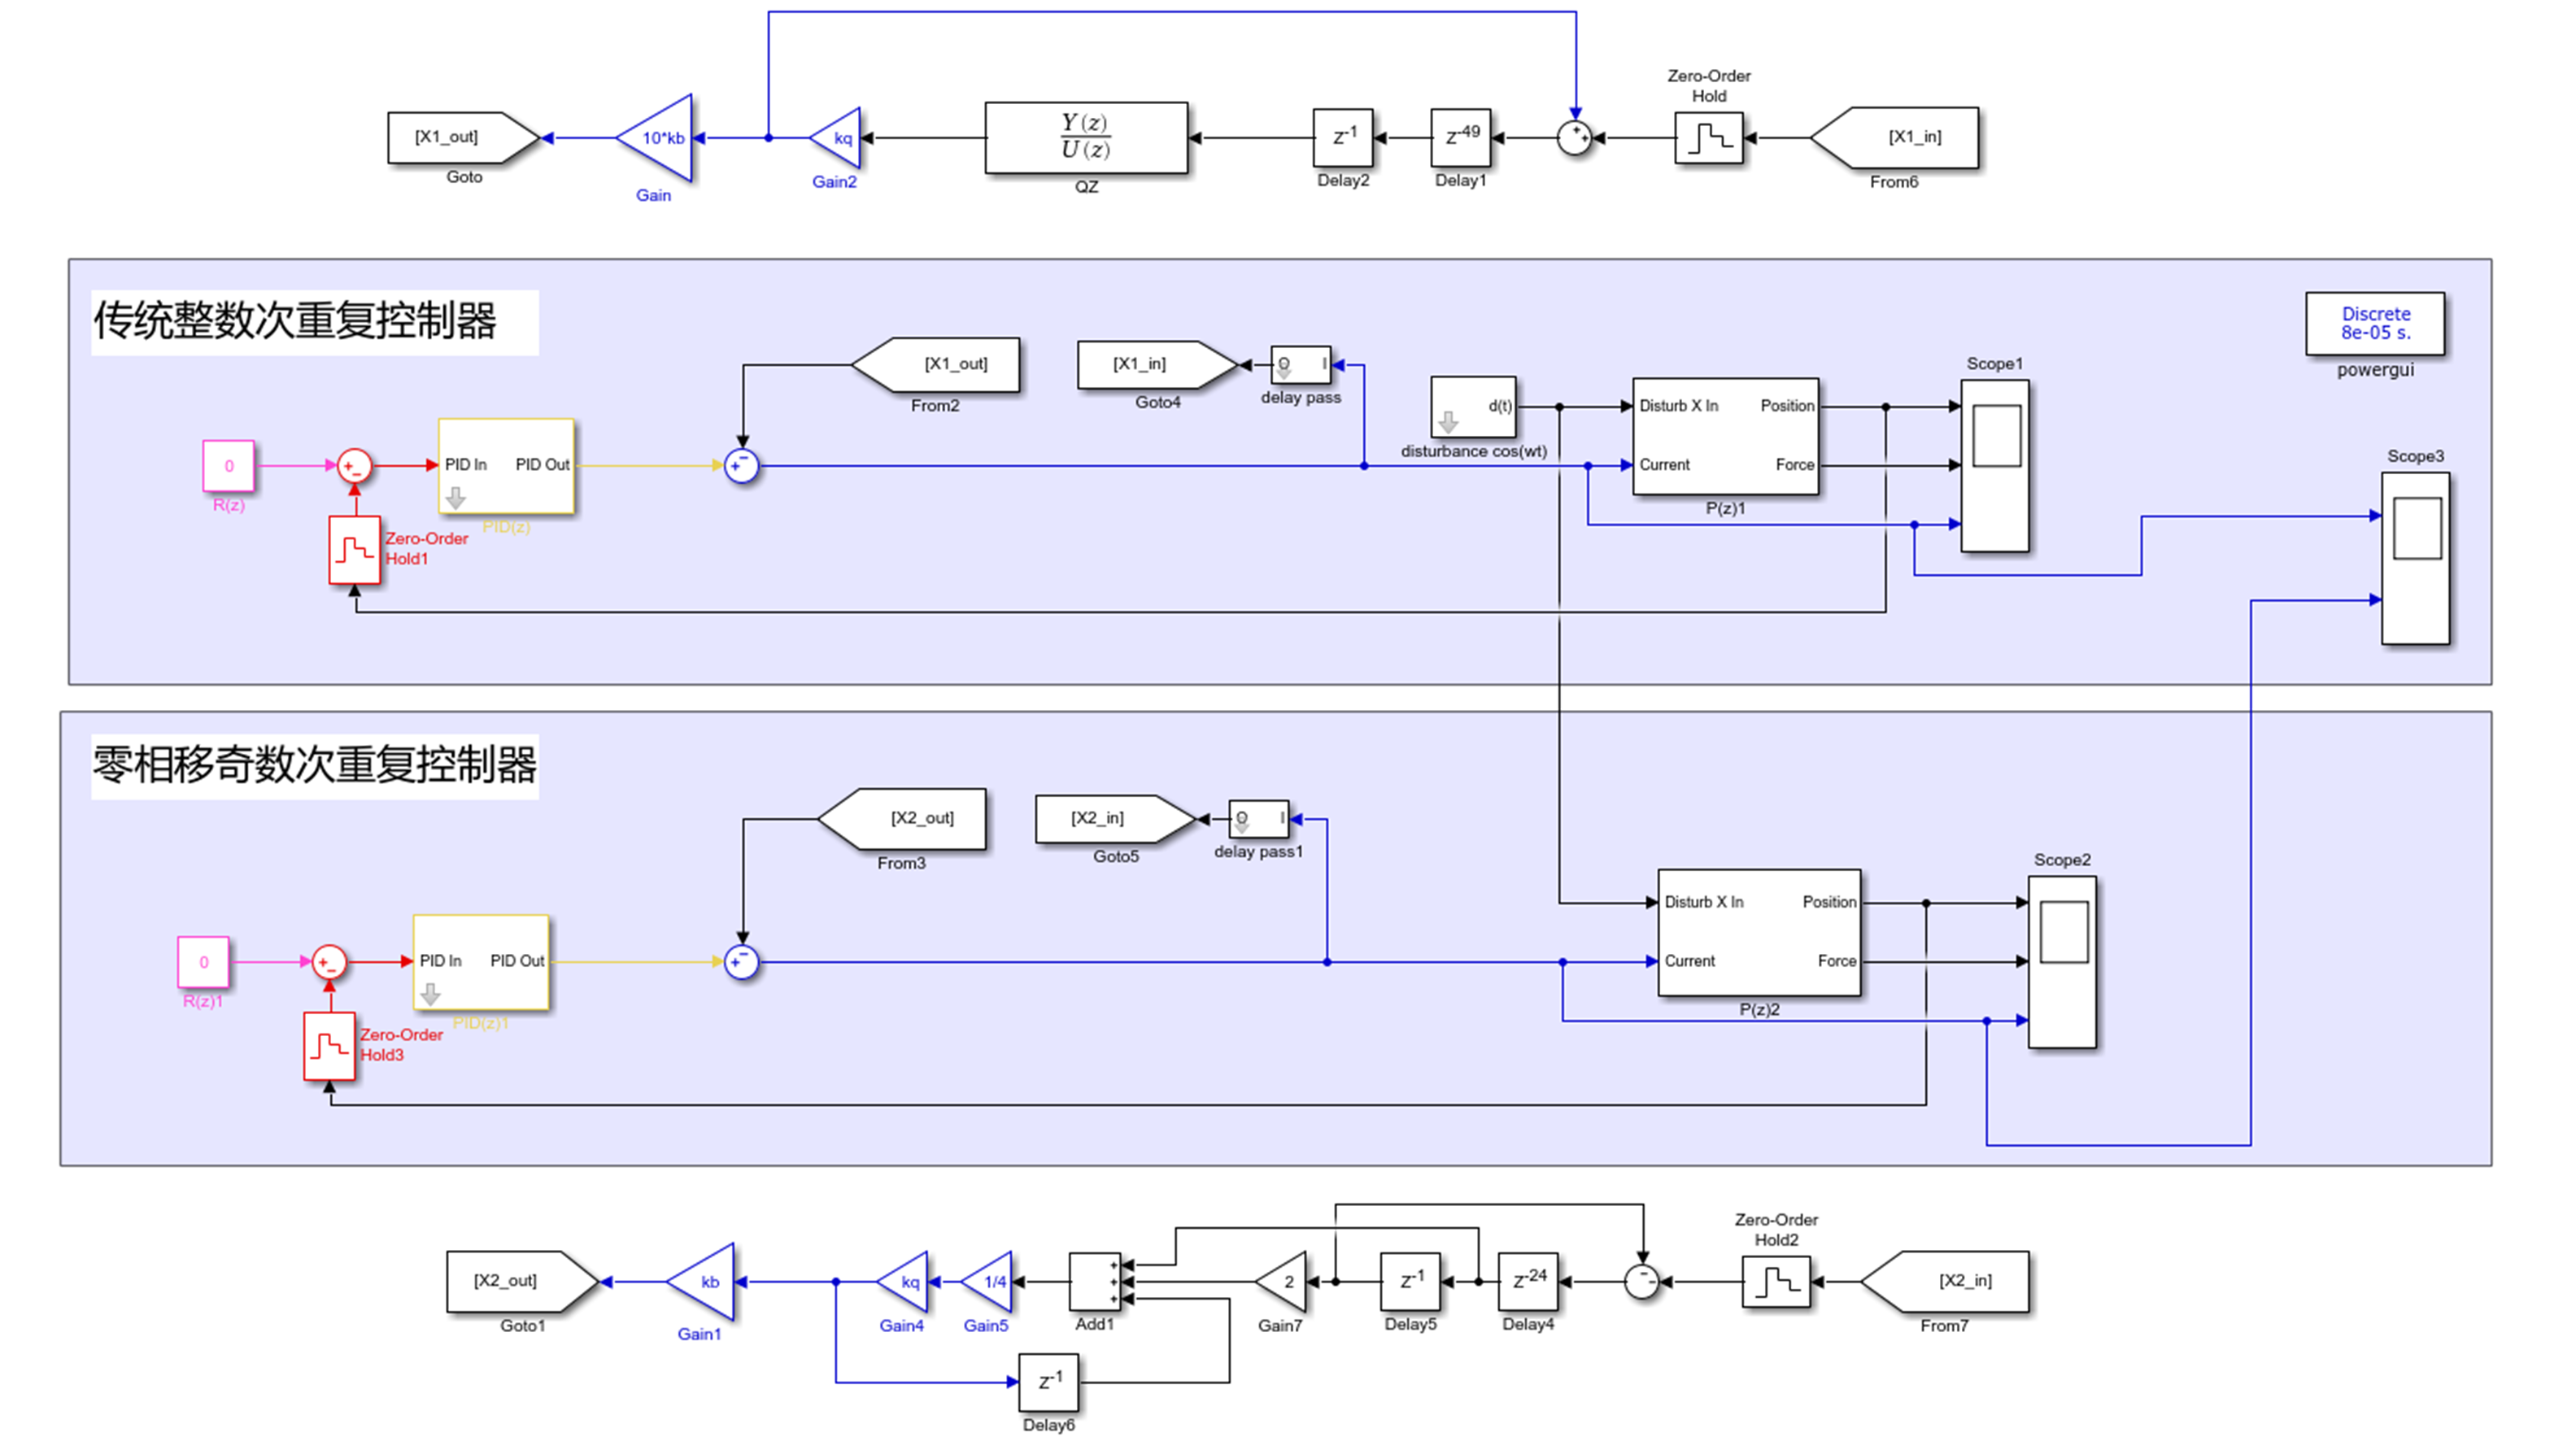
\includegraphics[scale=1.0]{3-simulink_model.png}
	\caption{CRC和ZORC仿真模型}
	\label{fig:3-simulink_model}
\end{figure}

\begin{figure}[h!]
	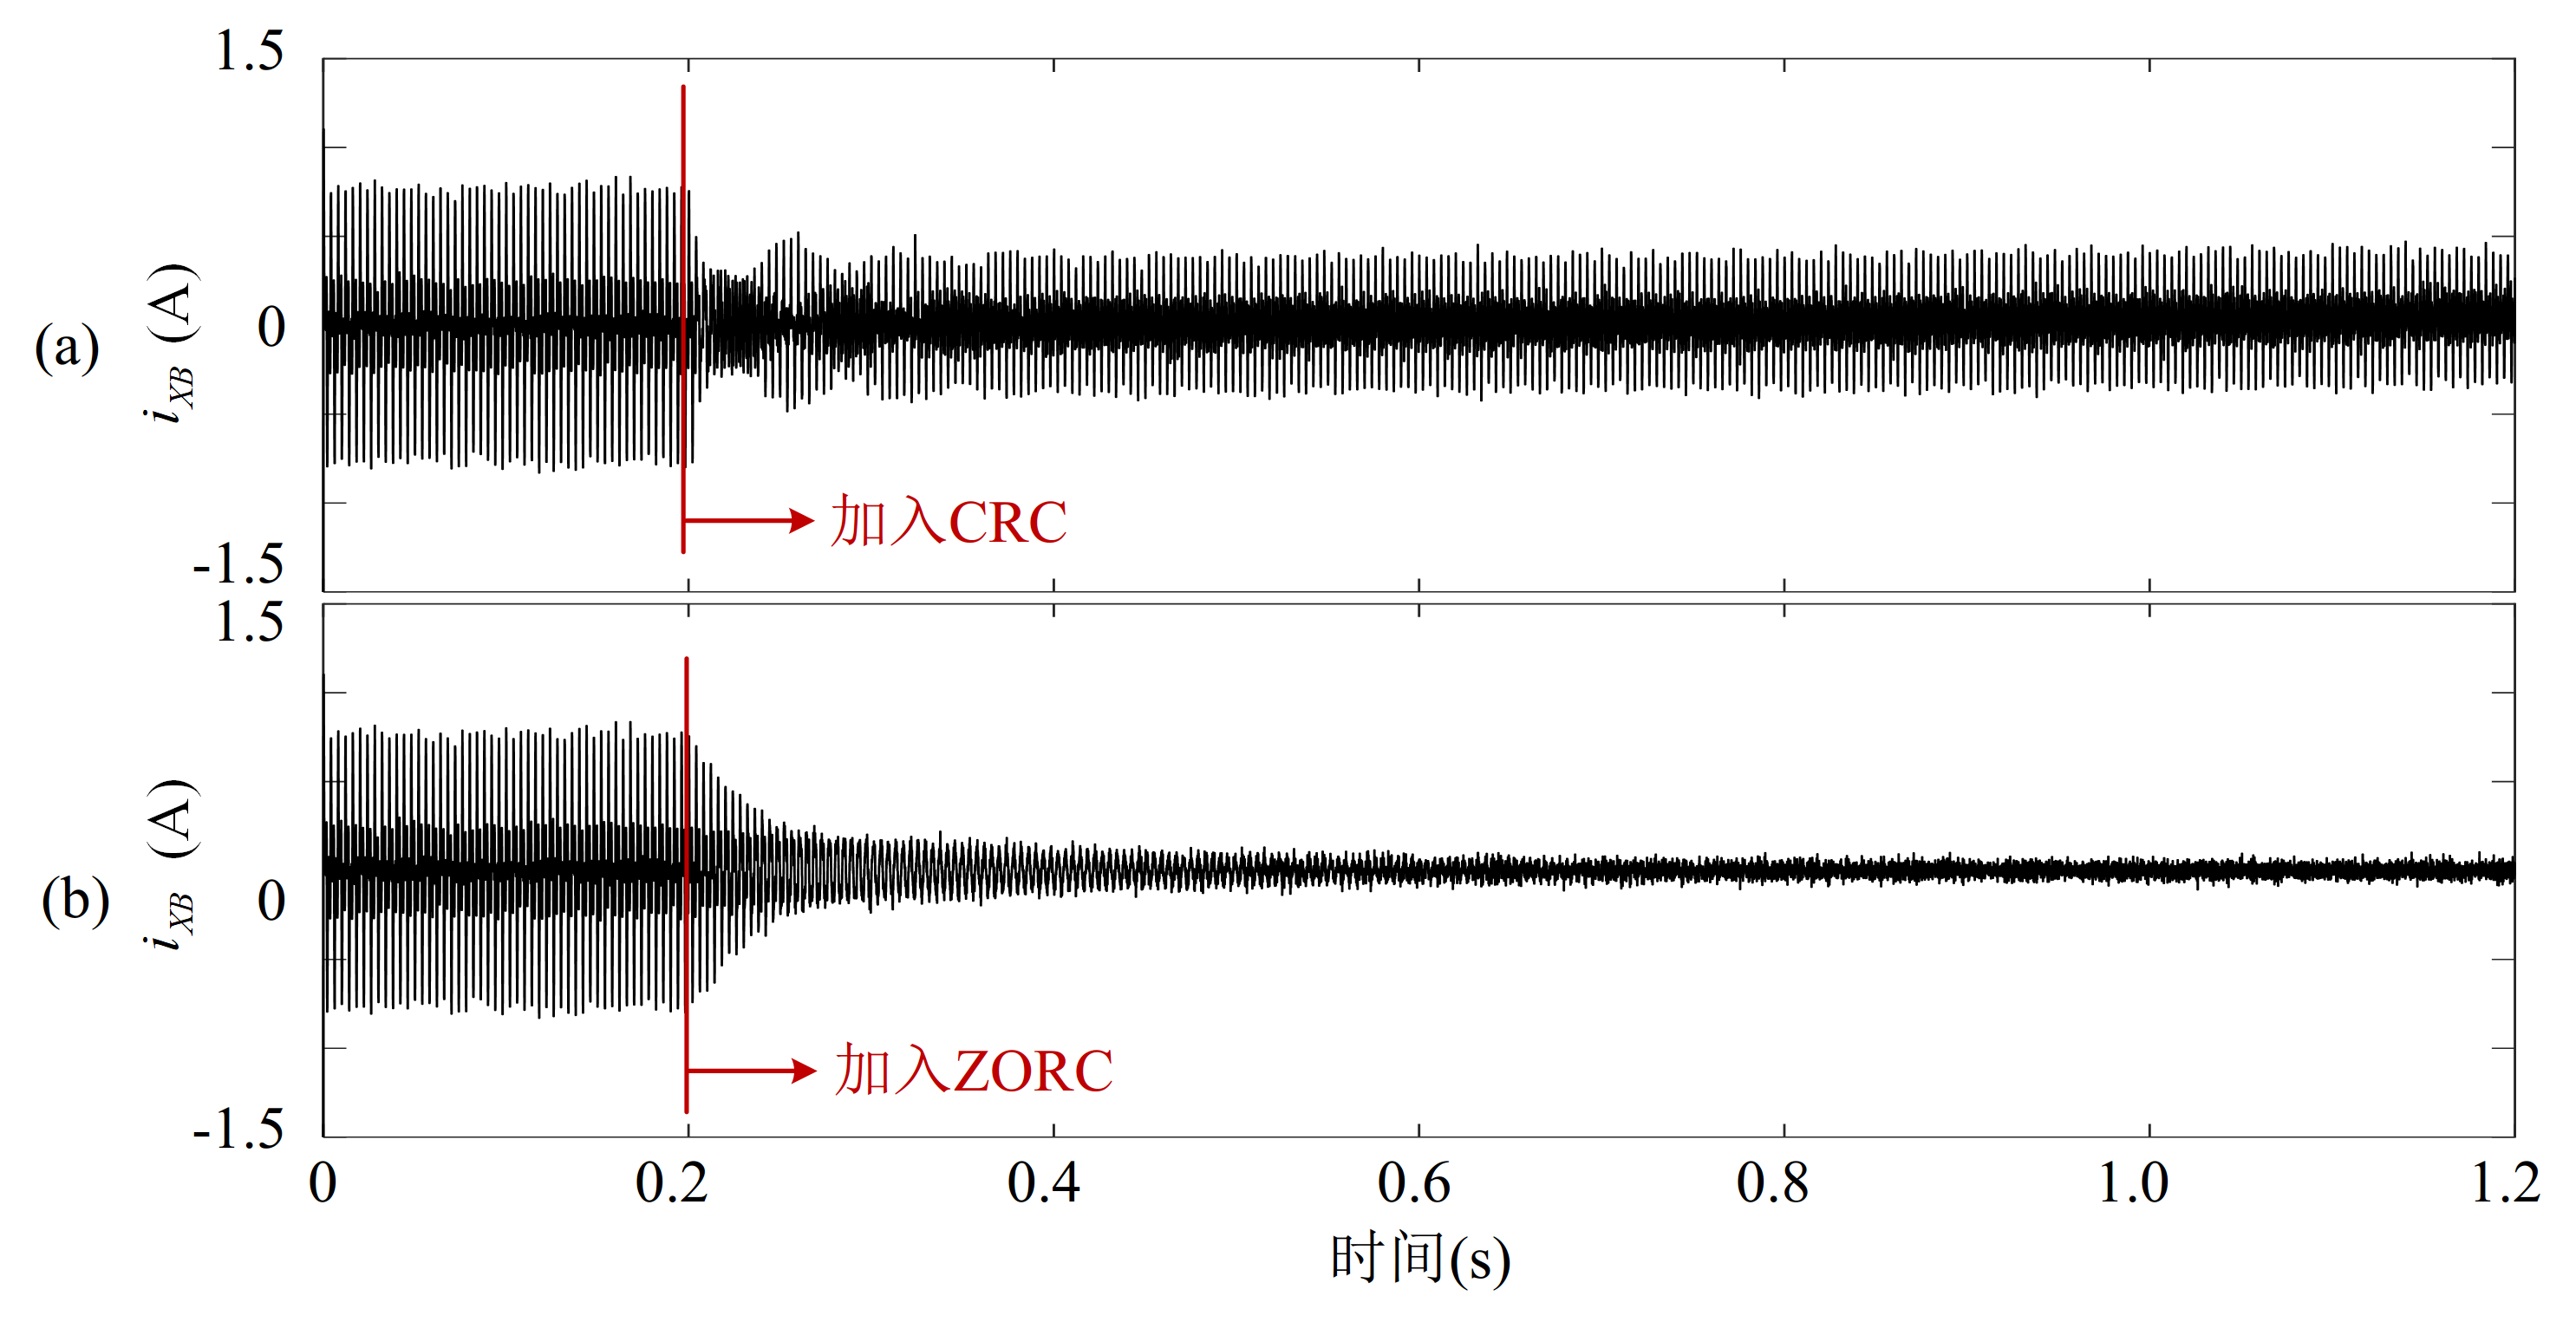
\includegraphics[scale=1.0]{3-current.png}
	\caption{加入CRC和ZORC的$i_{XB}$时域仿真波形:(a)加入CRC前后电流波形,(b)加入ZORC前后电流波形}
	\label{fig:3-current}
\end{figure}

\autoref{fig:3-2-crc}~和\autoref{fig:orc}~所对应的的仿真模型如\autoref{fig:3-simulink_model}~所示。在两个模型中注入含有谐波频率一致、各频率谐波的幅值一致的扰动信号,然后同时加入CRC和ZORC,观察加入重复控制器前后控制电流的变化。

从\autoref{fig:3-current}~可以看到,加入重复控制器前,扰动信号造成电流中存在幅值约为0.7A的交流成分。加入CRC后,谐波电流幅值下降到约0.4A;加入ZORC后,谐波电流幅值下降到约0.2A。两种情况下转子均未失稳。仿真结果说明ZORC可以有效抑制控制电流中的谐波分量,且比CRC的谐波抑制能力更强。

\begin{figure}[h!]
	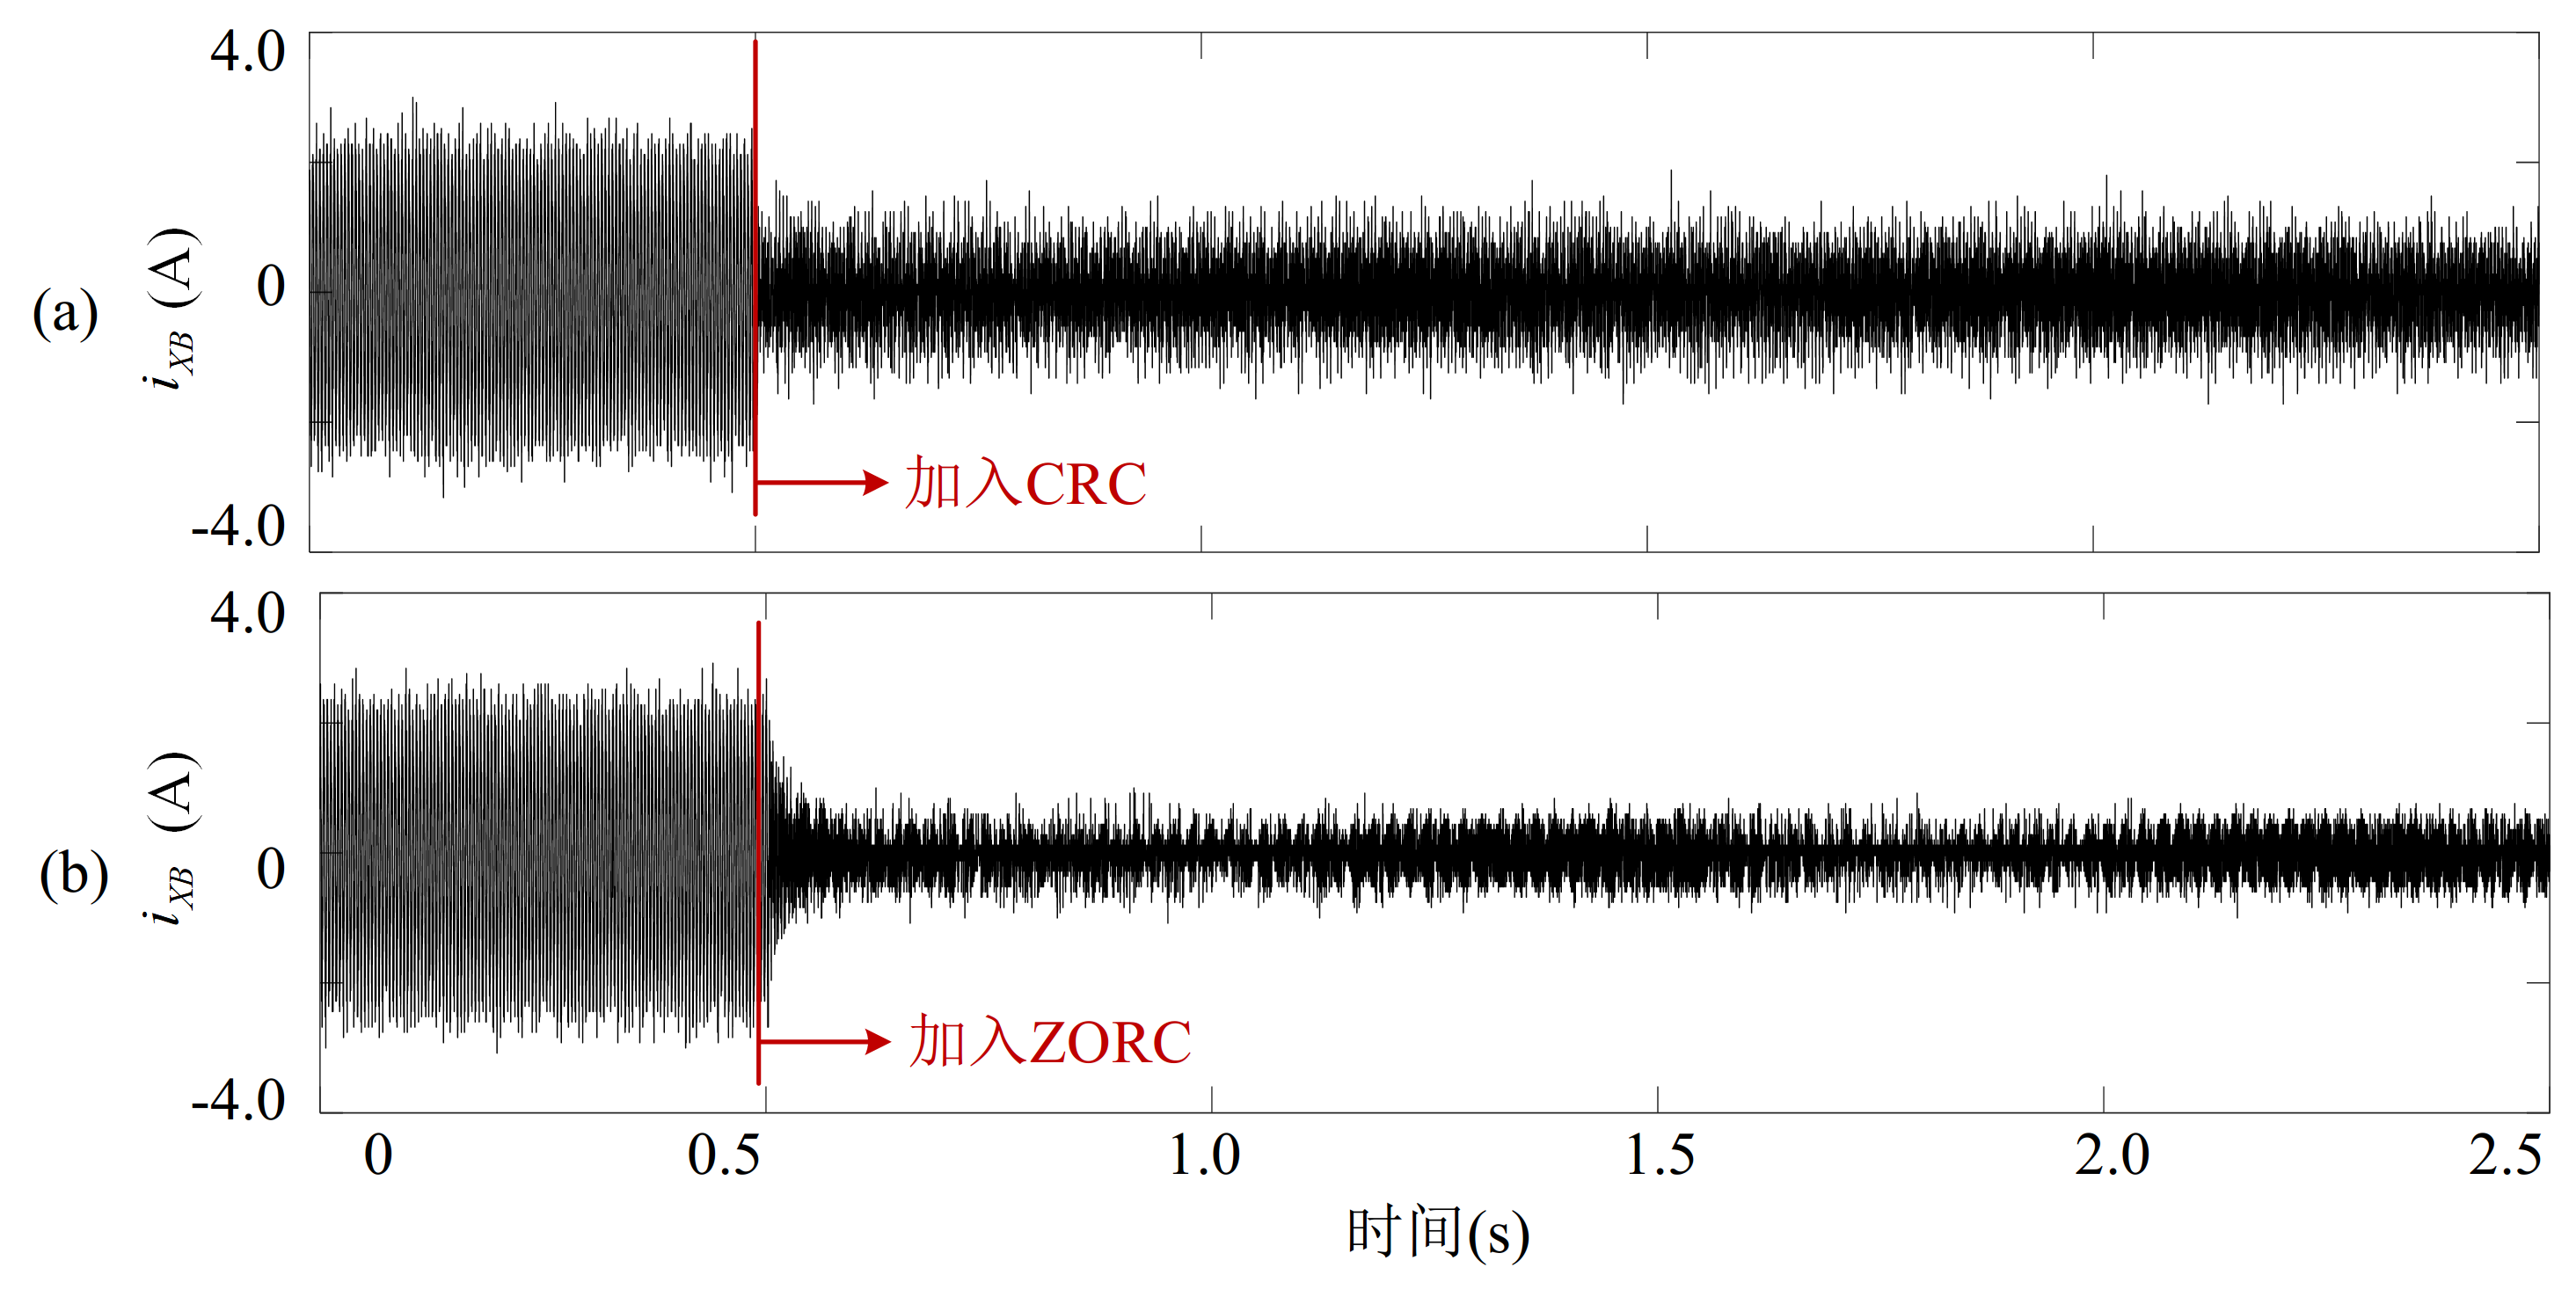
\includegraphics[scale=1.0]{5-orc_current.png}
	\caption{转子250Hz时的控制电流时域波形实验测量结果:(a)加入CRC前后电流波形,(b)加入ZORC前后电流波形}
	\label{fig:5-orc_current}
\end{figure}

\autoref{fig:5-orc_current}~显示了加入CRC和ZORC前后的电流波形。\autoref{fig:5-orc_current}a中可以看到加入CRC之前,控制电流的幅值约为0.7A,加入
CRC之后控制电流下降到约0.4A。\autoref{fig:5-orc_current}b中,加入ZORC之后,控制电流从0.7A下降到约0.2A。控制电流的时域波形表明加入ZORC更能抑制控制电流中的谐波分量。

\begin{figure}[h!]
	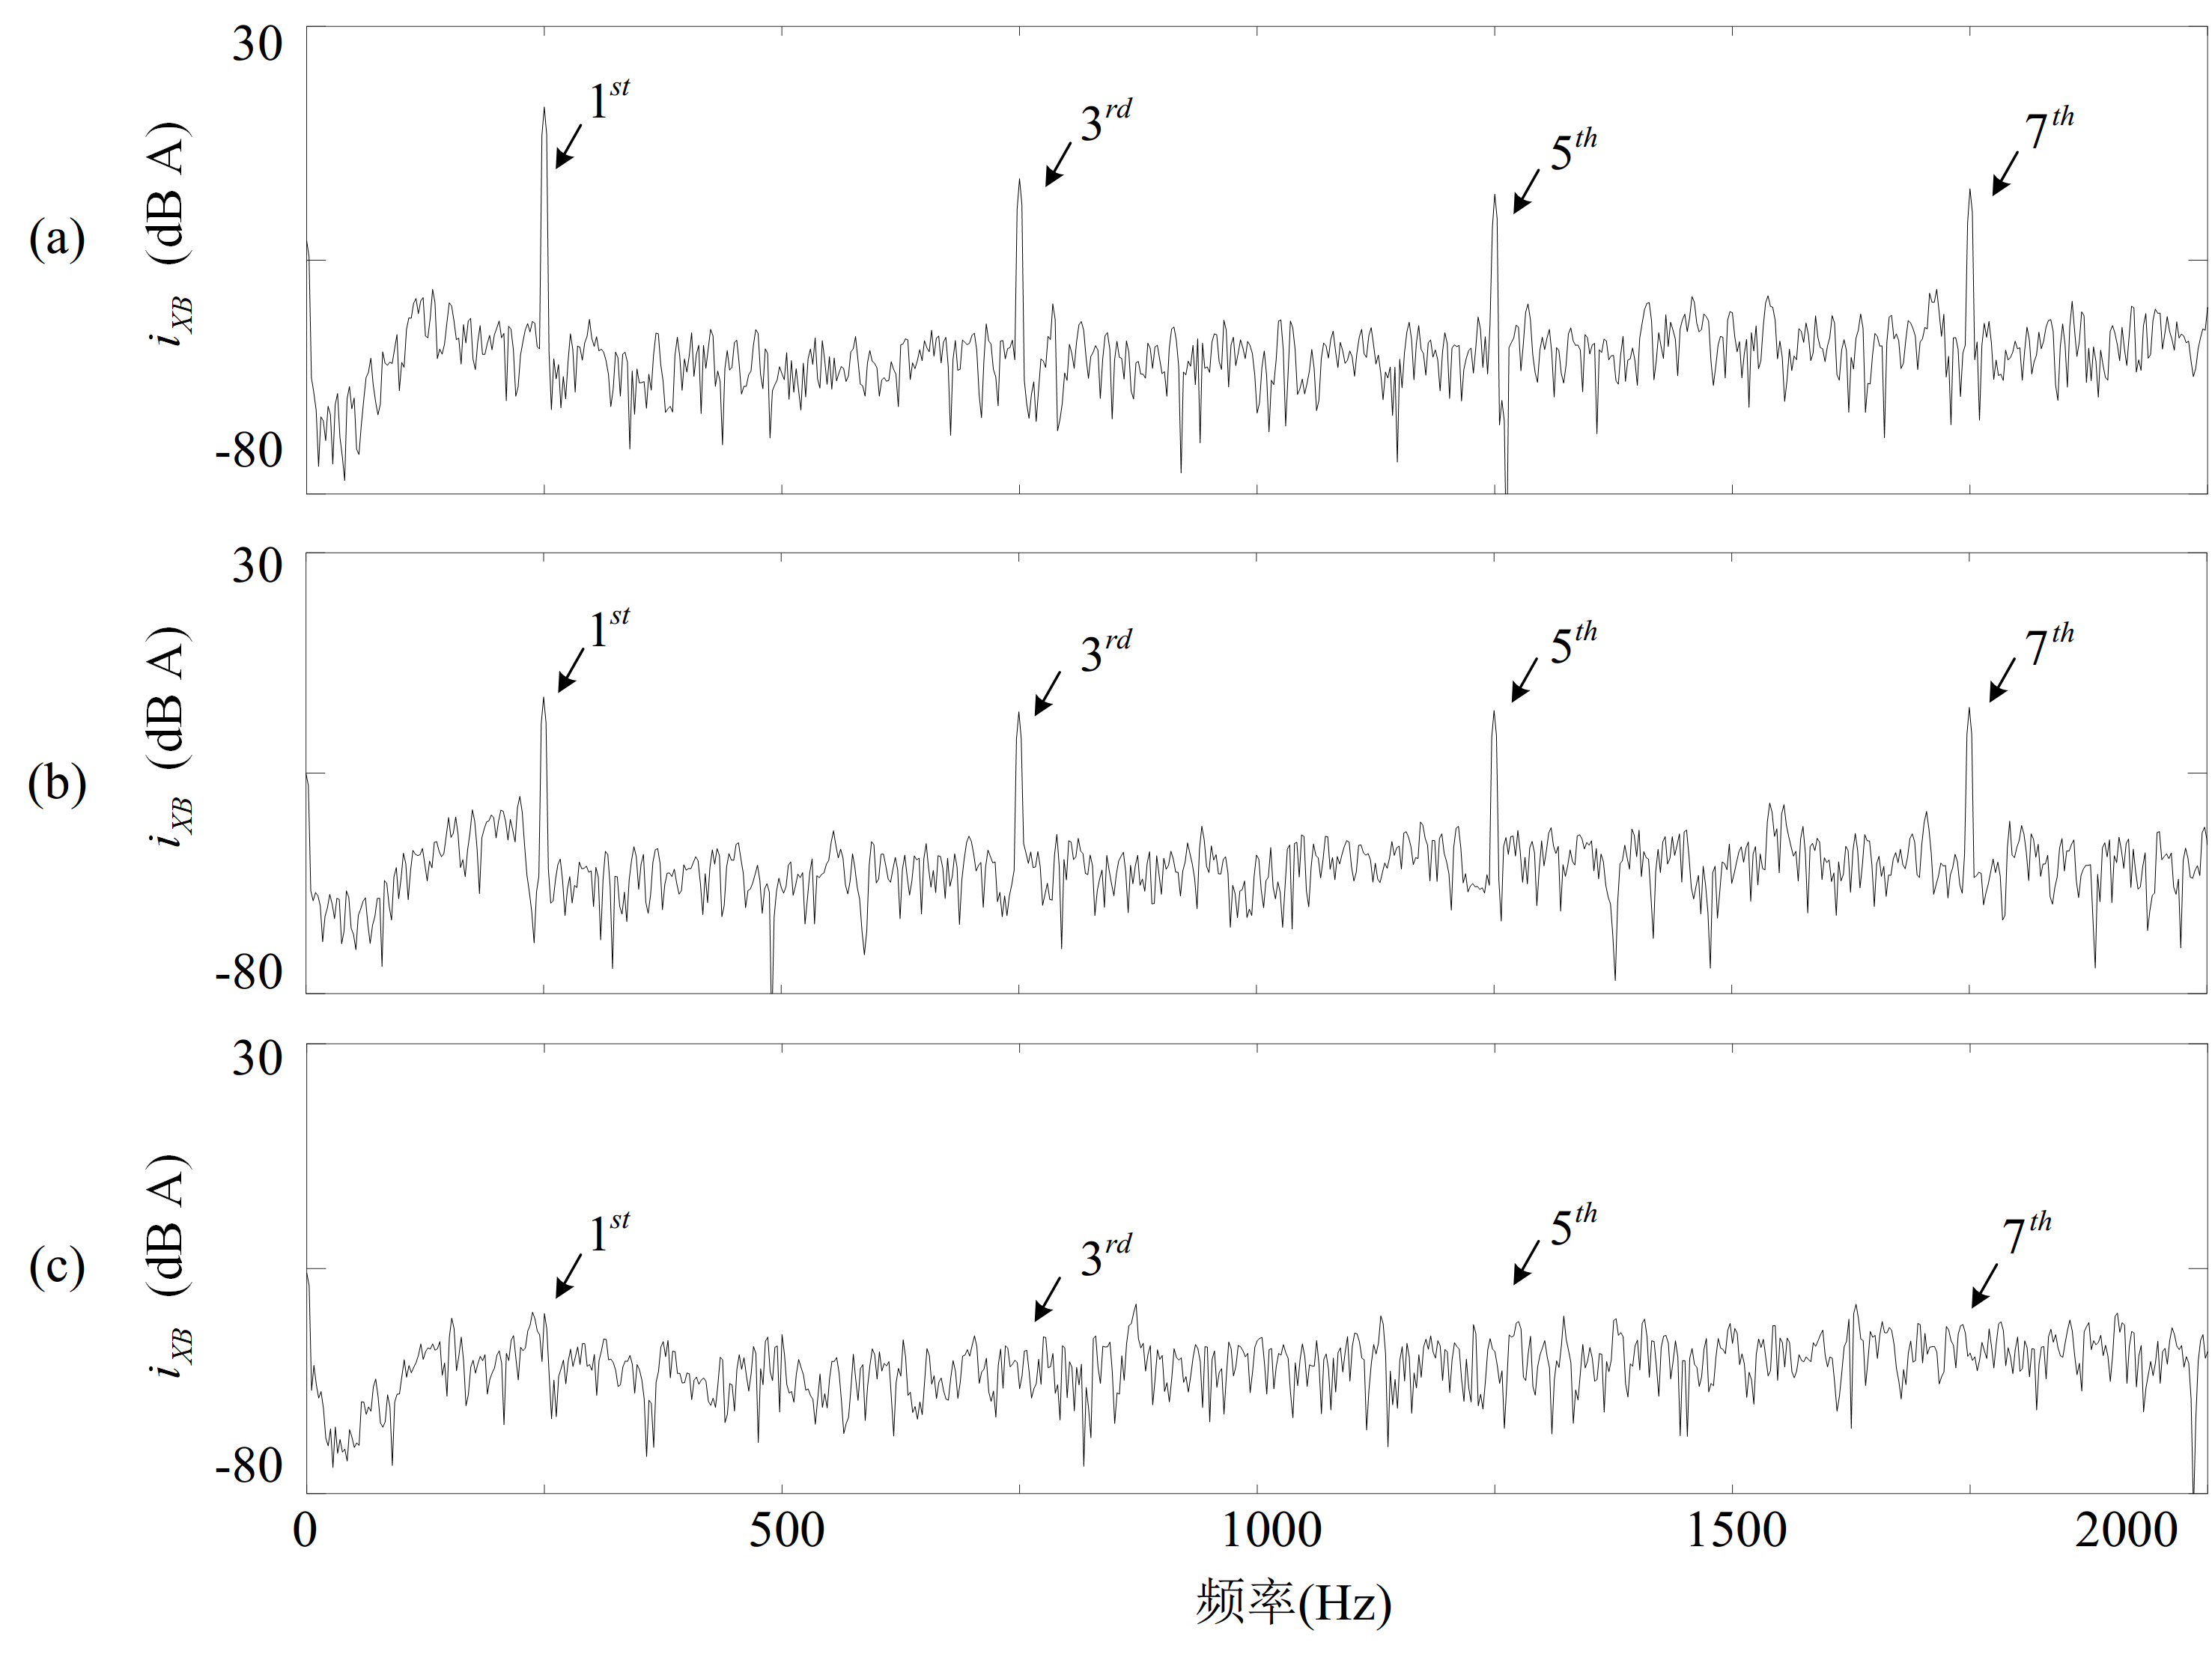
\includegraphics[scale=1.0]{5-orc_current_fft.png}
	\caption{转子250Hz时的控制电流频谱实验测量结果:(a)PID,(b)PID+CRC,(c)PID+ZORC}
	\label{fig:5-orc_current_fft}
\end{figure}

为了定量分析ZORC在各个谐波频率处的抑制能力,对\autoref{fig:5-orc_current}~的时域波形做傅里叶频谱分析,观察时域电流的频谱。\autoref{fig:5-orc_current_fft}a显示在仅有PID控制下,由质量不平衡和传感器误差引入的谐波电流的一、三、五、七次谐波的幅值分别是2.8dB、-12.5dB、-15.8dB和-14.7dB。\autoref{fig:5-orc_current_fft}b中,加入传统整数次重复控制器之后,幅值分别下降到-12.7dB、-16.1dB、-15.8dB和-15.1dB。可以看出,随着谐波频率的升高,CRC的抑制能力逐渐减弱。\autoref{fig:5-orc_current_fft}c中,加入ZORC之后,谐波幅值分别下降至-40.0dB、-56.7dB、-48.4dB和-48.8dB,下降程度均超过90\%。

\begin{table}[htb]
  \caption[250Hz时磁悬浮轴承系统功率实验测量结果]{250Hz时磁悬浮轴承系统功率实验测量结果\label{tab:amb_power}}
  \begin{tabular}{cc}
    \toprule
    控制策略 & 功率消耗 \\
    \midrule
    PID & 142.3W\\
    PID+CRC & 95.3W\\
    PID+ZORC & 58.2W\\
    \bottomrule
  \end{tabular}
\end{table}

\autoref{tab:amb_power}~显示了磁悬浮轴承系统在转子250Hz悬浮运转时的功率消耗。仅有PID控制时,系统功率消耗为142.3W;当加入CRC之后,功率消耗下降到95.3W;当加入ZORC之后,功率消耗则下降到58.2W。该对比结果显示ZORC比CRC更能降低系统的功率消耗。

\begin{figure}[h!]
	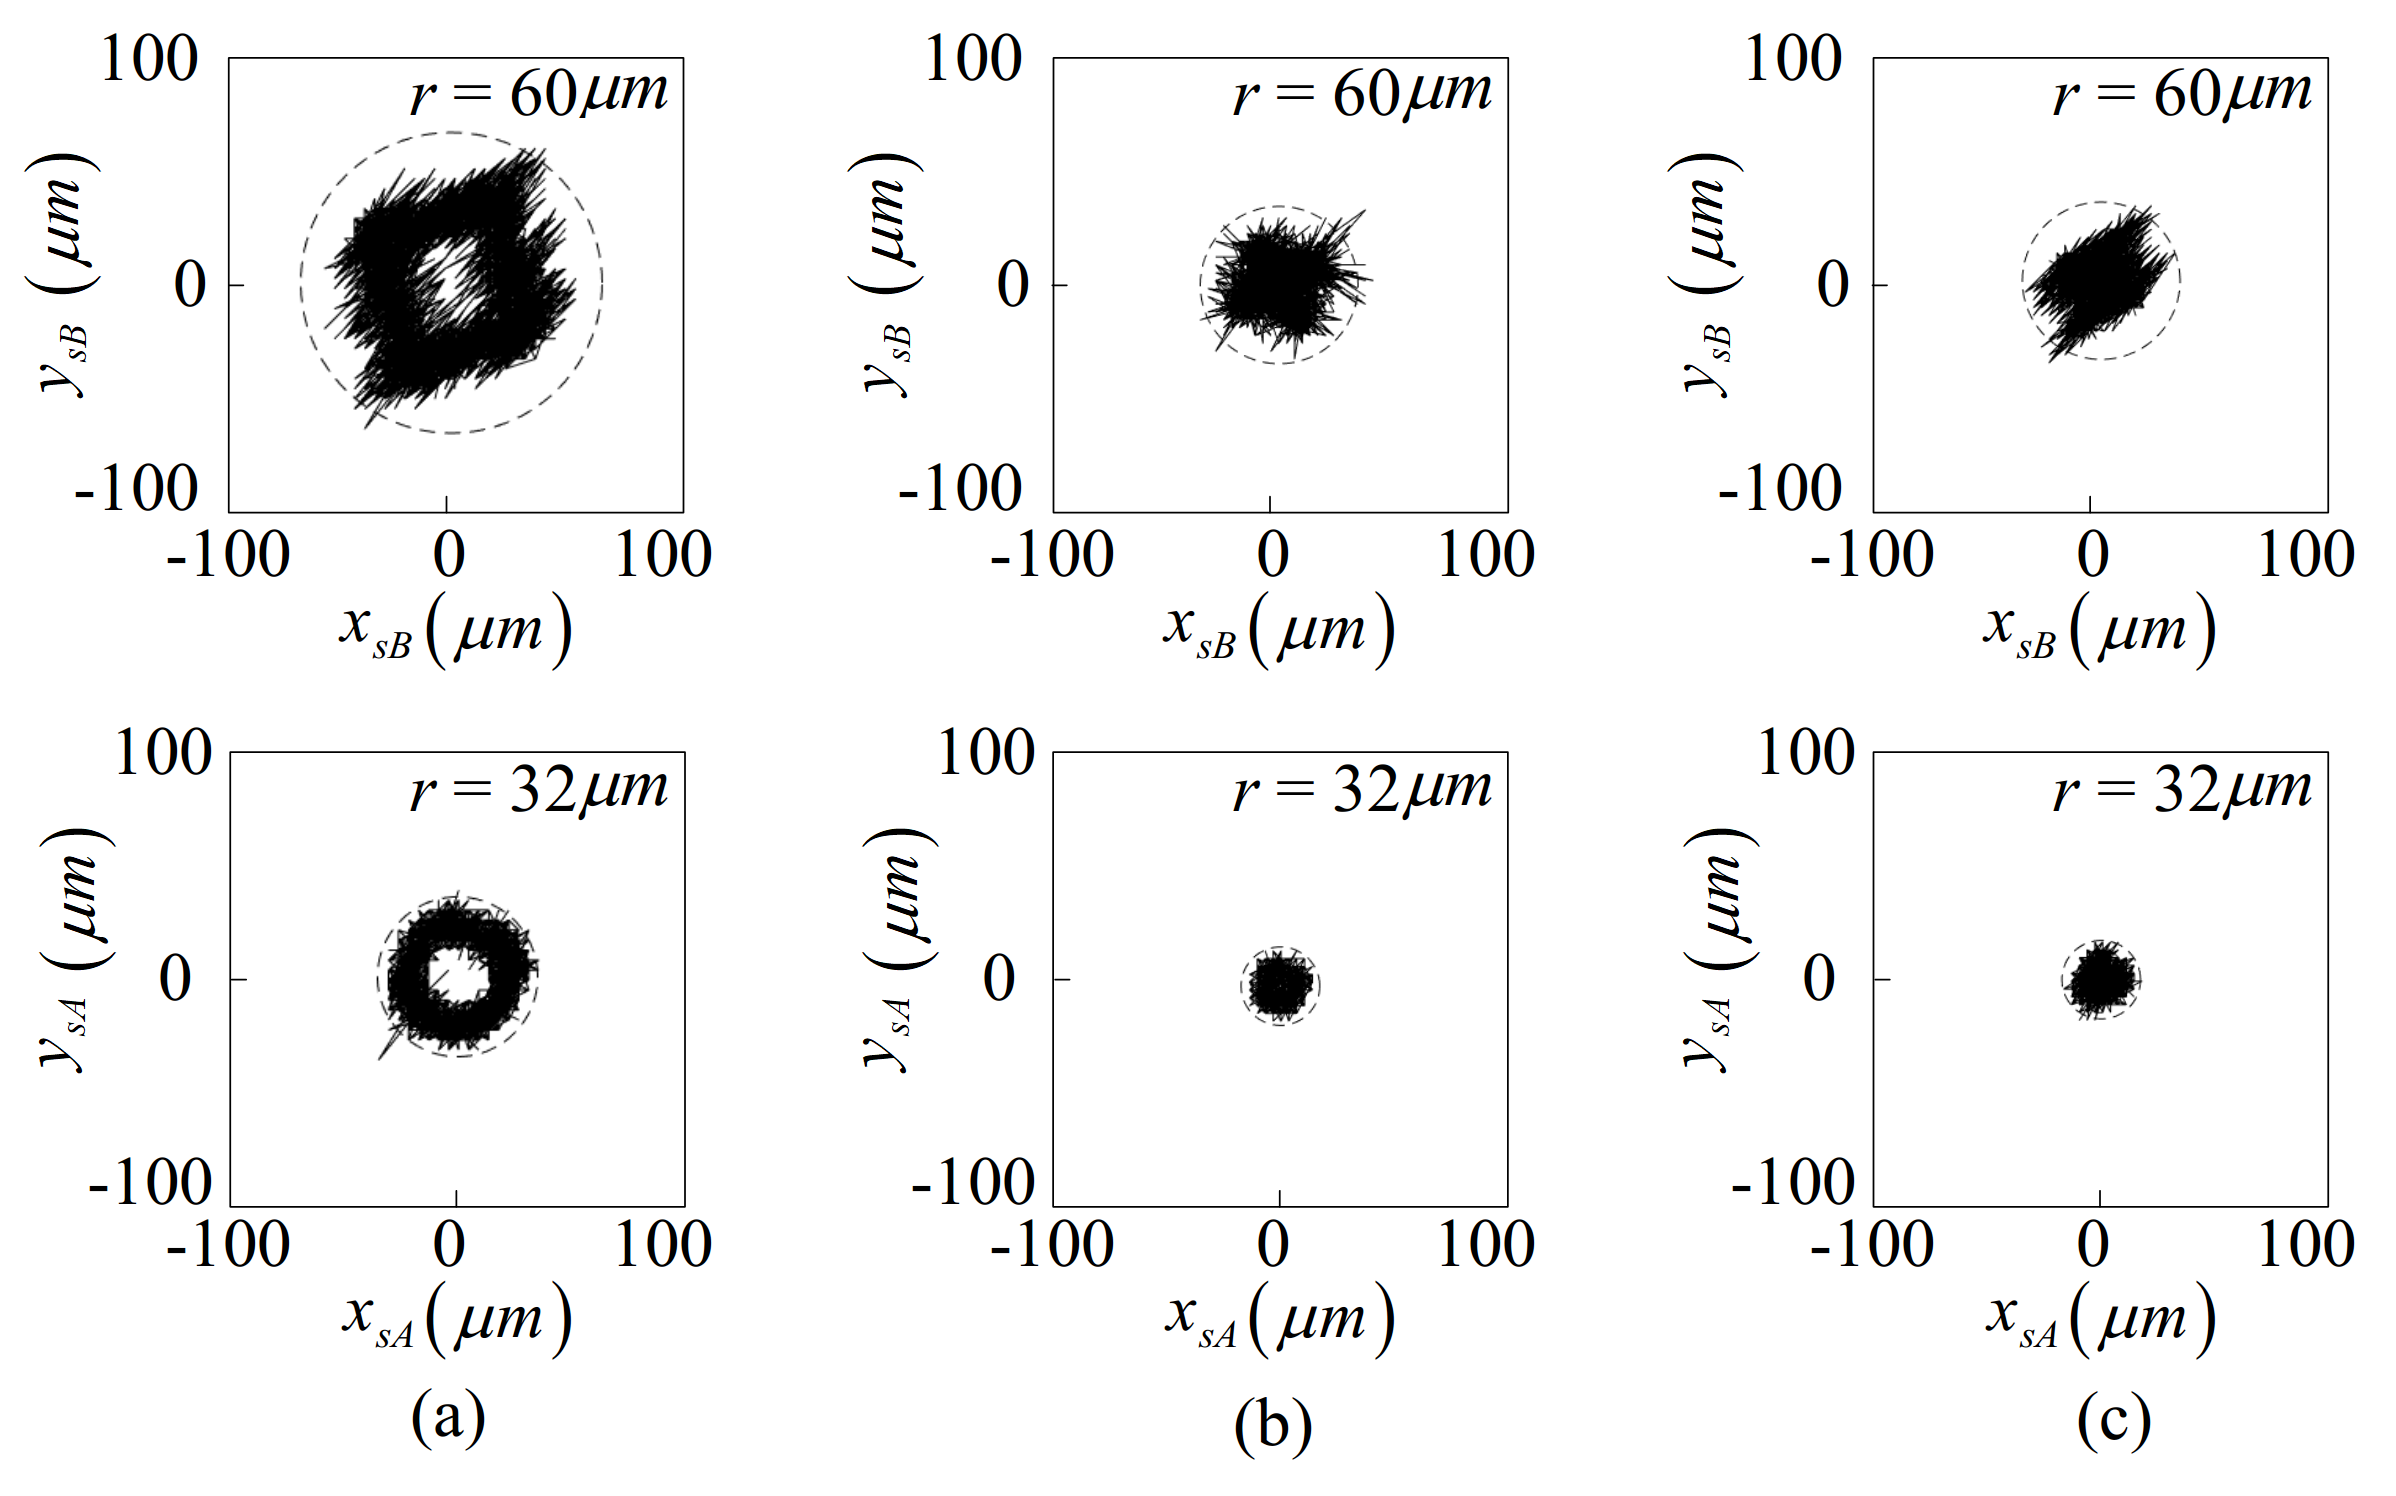
\includegraphics[scale=1.0]{5-rotor_locus.png}
	\caption{转子250Hz时两端的轴心轨迹实验测量结果:(a)PID,(b)PID+CRC,(c)PID+ZORC}
	\label{fig:5-rotor_locus}
\end{figure}

除功率消耗降低之外,ZORC带来的好处是提升转子的回转精度。此处的轴心轨迹通过位移传感器测得的转子位移绘制而成,轴心轨迹的半径记为$r$。\autoref{fig:5-rotor_locus}a显示仅有PID控制下,转子在A端磁悬浮轴承处的振动位移幅值为$60\mu m$,在B端磁悬浮轴承处的振动位移幅值为$32\mu m$。\autoref{fig:5-rotor_locus}b中,加入CRC之后,转子在A端磁悬浮轴承处的振动位移幅值下降到$40\mu m$,在B端磁悬浮轴承处的振动位移幅值下降到$20\mu m$。\autoref{fig:5-rotor_locus}c中,加入ZORC之后,转子在A端和B端磁悬浮轴承处的振动位移幅值同样下降到$40\mu m$和$20\mu m$。该实验现象说明CRC和ZORC具有相同的提升转子回转精度的能力。

\begin{figure}[h!]
	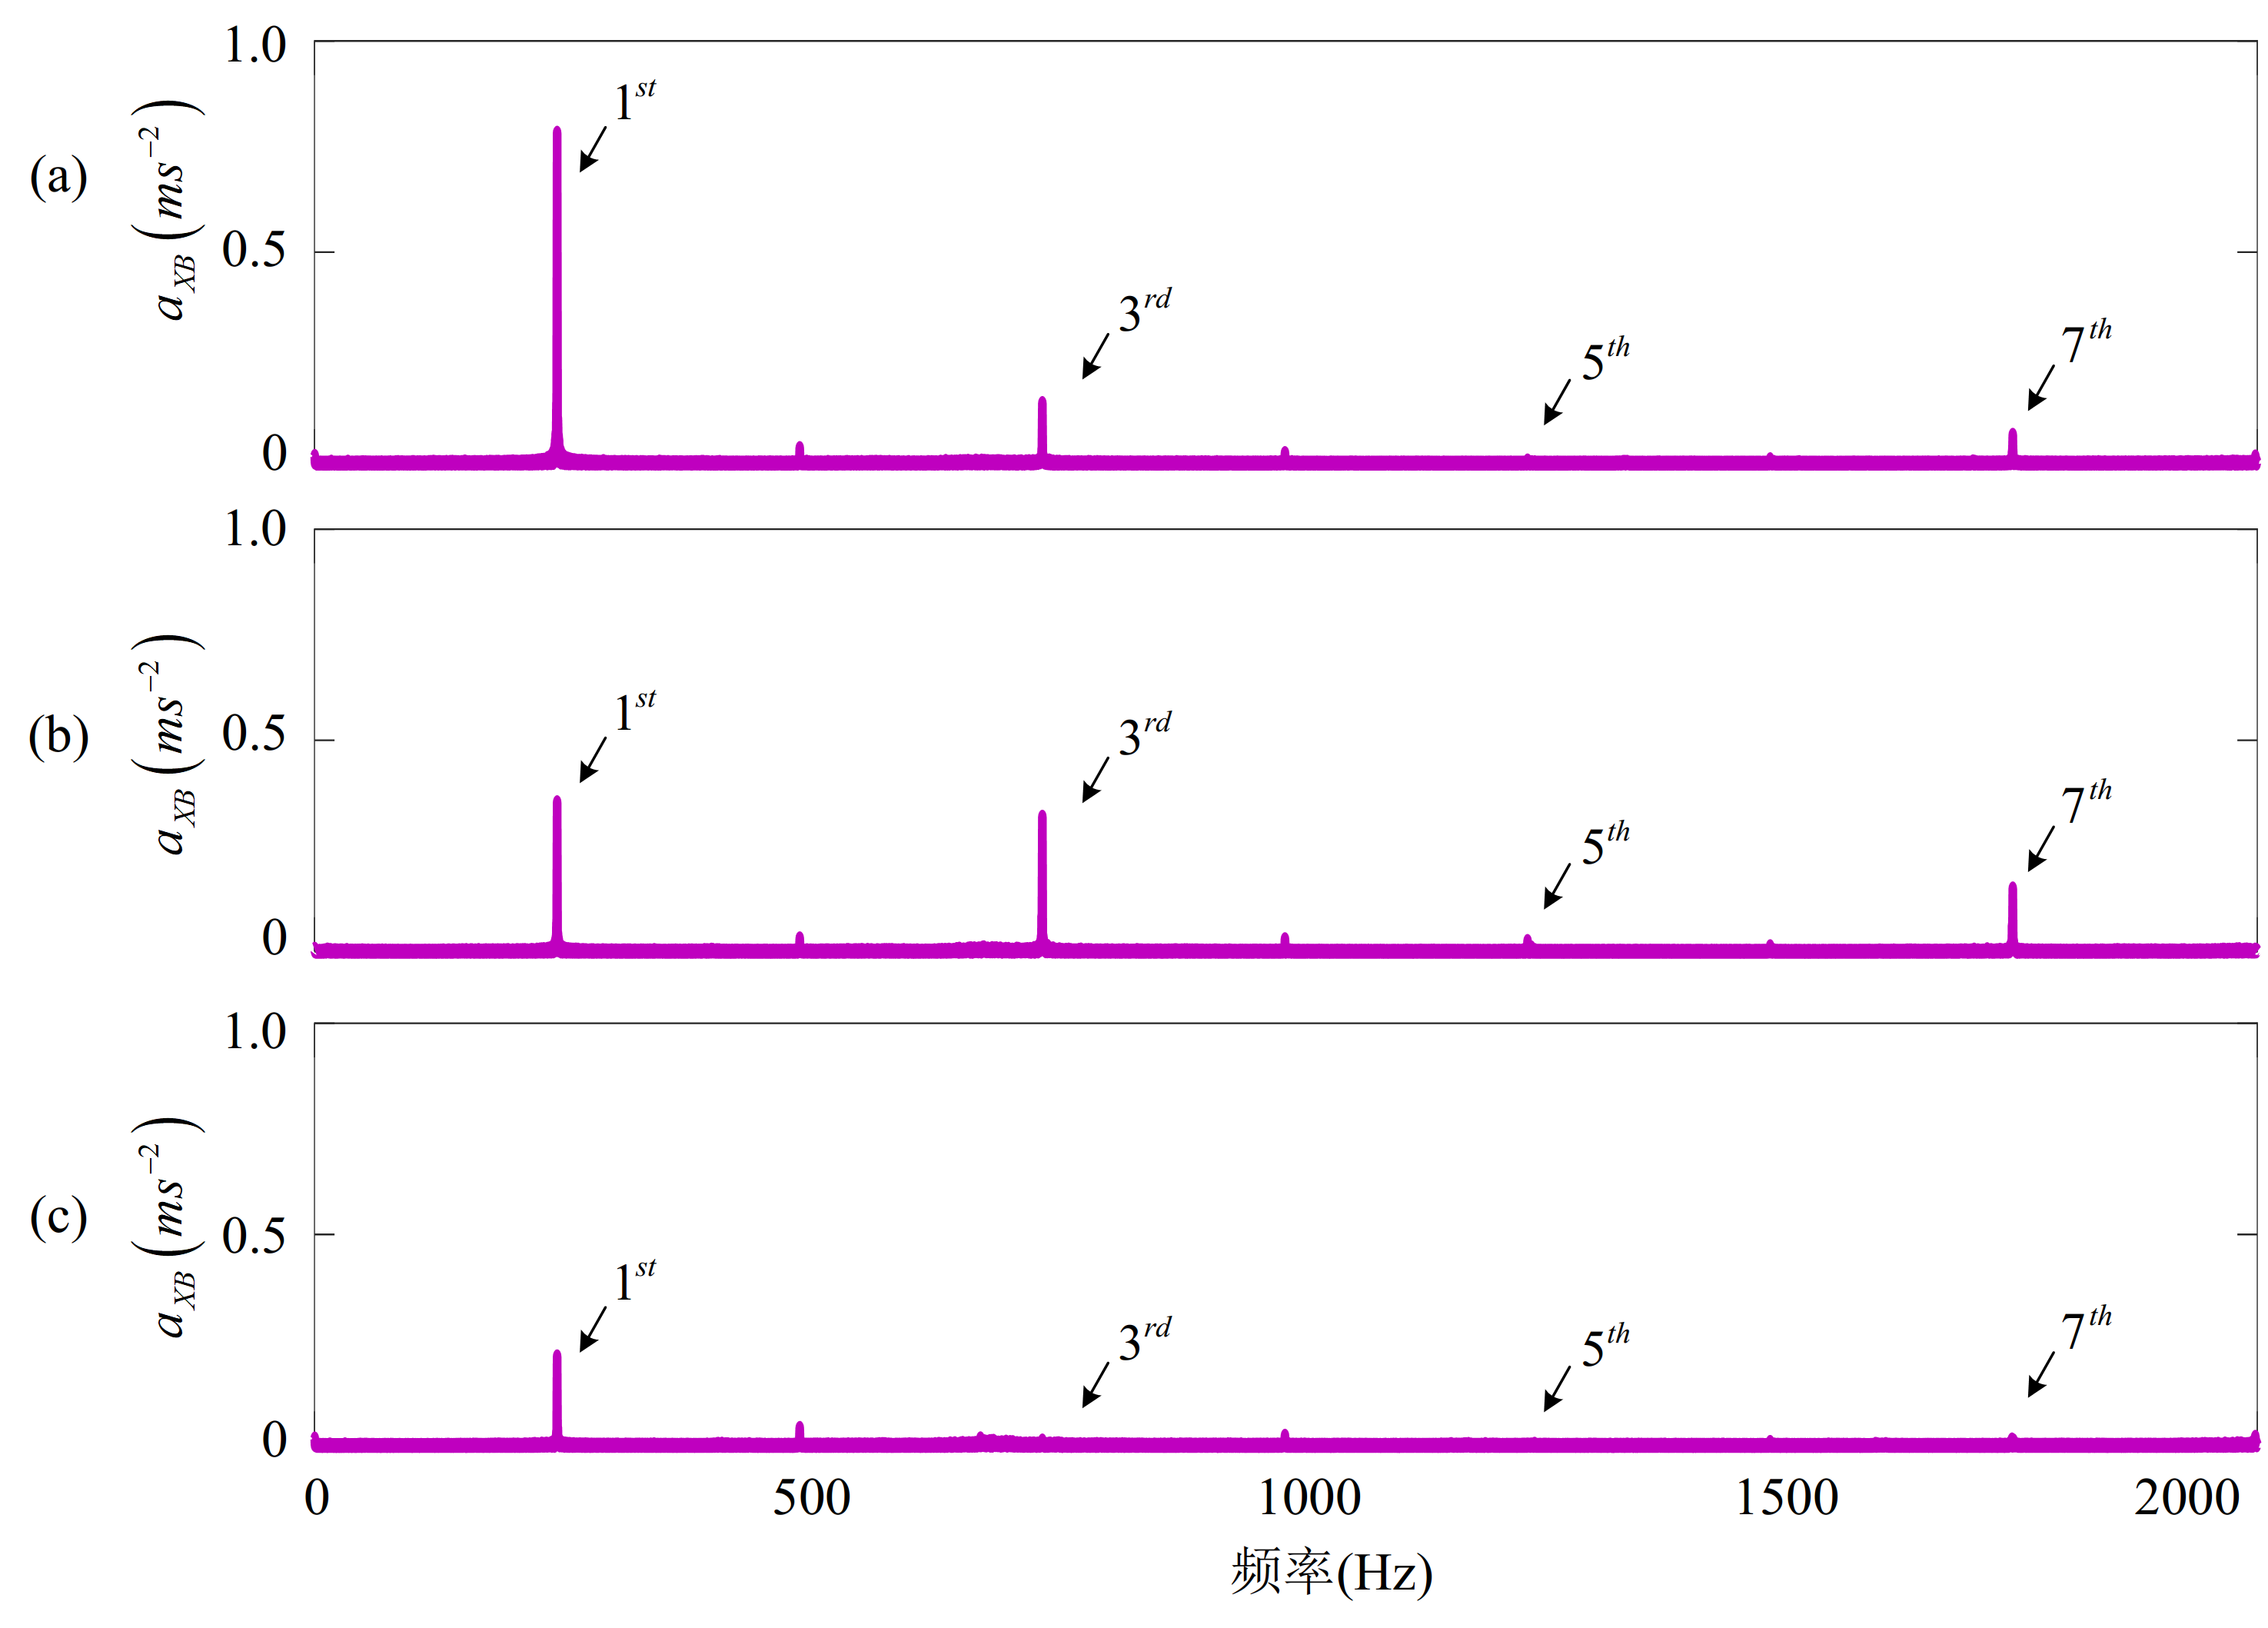
\includegraphics[scale=1.0]{5-orc_acc.png}
	\caption{转子250Hz时定子基座的加速度实验测量结果:(a)PID,(b)PID+CRC,(c)PID+ZORC}
	\label{fig:5-orc_acc}
\end{figure}

为了验证实际应用过程中ZORC对整机振动力的抑制能力,我们使用加速度传感器来测量磁悬浮电机机壳上的振动加速度。
\autoref{fig:5-orc_acc}~显示了转子250Hz时定子基座的加速度实验测量结果。\autoref{fig:5-orc_acc}a显示当仅有PID控制时,一、三、五、七次谐波频率处的振动幅值为$0.782ms^{-2}$、$0.142ms^{-2}$、$0.002ms^{-2}$和$0.066ms^{-2}$。\autoref{fig:5-orc_acc}b中,加入CRC之后,与转速同频的振动幅值下降到$0.352ms^{-2}$,然而三、五、七次谐波频率处的振动幅值上升到$0.318ms^{-2}$、$0.024ms^{-2}$、$0.148ms^{-2}$。这是因为尽管三、五、七次谐波频率处的电流幅值有轻微的衰减,其相位可能发生剧烈的改变,因此使得磁悬浮力增大。\autoref{fig:5-orc_acc}c中,加入ZORC之后,一、三、五、七次谐波频率处的振动幅值下降到$0.210ms^{-2}$、$0.011ms^{-2}$、$0.001ms^{-2}$和$0.014ms^{-2}$,与转速同频的振动力下降了超过70\%,其它谐波频率处的振动力几乎下降到零。该实验现象说明CRC的谐波抑制能力随着频率升高而减弱,与之对比的是ZORC可以有效抑制所有频率处的谐波。
\section{本章小结}
本章提出了ZORC解决CRC存在相位延迟进而导致其在磁悬浮轴承应用中谐波抑制能力不足的问题。对比分析比较了CRC和ZORC的工作原理和稳定性分析方法。基于ZORC的主动振动抑制方法的仿真和实验说明:与CRC相比,ZORC可以更加深度地抑制基波和谐波电流、降低基座振动力。

\chapter{基于重复控制器的现场动平衡方法}
针对主动振动抑制算法无法同时实现振动位移最小和振动力最小的目标,本章提出一种基于ZORC的现场动平衡方法。分析磁悬浮轴承中转子常用的两类现场动平衡方法:需试重的现场动平衡方法和无需试重的现场动平衡方法,阐述了基于ZORC的现场动平衡方法的谐波抑制、偏心距辨识、校正质量计算步骤。

\section{需试重的现场动平衡方法}

\subsection{影响系数法}

影响系数法是机械转子中应用范围较广的一种动平衡方法。对于较长的转子,需要采用双面增重平衡的影响系数法,该方法的实现思路如下:设系统有$SA$和$SB$两个转子位移信号检测面,$CA$和$CB$两个质量校正面。选定转子稳定运行、振动幅值适中的转速$\Omega _0$作为不平衡测试转速。影响系数法操作步骤为:

(1)在$\Omega _0$时,测试得到转子在$SA$和$SB$处的位移振动矢量为${\boldsymbol{A_0}}$和${\boldsymbol{B_0}}$;

(2)在$CA$面加试重${\boldsymbol{C_A}}$,在$\Omega _0$时,测试得到转子在$SA$和$SB$处的位移振动矢量为${\boldsymbol{A_A}}$和${\boldsymbol{B_A}}$。取下试重${\boldsymbol{C_A}}$;

(3)在$CB$面加试重${\boldsymbol{C_B}}$,在$\Omega _0$时,测试得到转子在$SA$和$SB$处的位移振动矢量为${\boldsymbol{A_B}}$和${\boldsymbol{B_B}}$。取下试重${\boldsymbol{C_B}}$;

(4)根据上述试重及振动矢量信息,解算出在$CA$面加校正质重${\boldsymbol{M_A}}$,在$CB$面加校正质重${\boldsymbol{M_B}}$,使得转子在全转速下的位移振动幅值为零。

其中根据试重及振动矢量信息解算校正质量的步骤如下:设$CA$面试重质量对$SA$和$SB$处位移振动的影响系数分别为$a_A$和$b_A$,$CB$面试重质量对$SA$和$SB$处位移振动的影响系数分别为$a_B$和$b_B$。则
\begin{equation}
\left\{
\begin{aligned}
&	{\boldsymbol{a_A}} = \frac{{\boldsymbol{A_A}}-{\boldsymbol{A_0}}}{{\boldsymbol{C_A}}} \\
&		{\boldsymbol{b_A}} = \frac{{\boldsymbol{B_A}}-{\boldsymbol{B_0}}}{{\boldsymbol{C_A}}}
\end{aligned}
\right.
\end{equation}

\begin{equation}
\left\{
\begin{aligned}
&	{\boldsymbol{a_B}} = \frac{{\boldsymbol{A_B}}-{\boldsymbol{A_0}}}{{\boldsymbol{C_B}}} \\
&		{\boldsymbol{b_B}} = \frac{{\boldsymbol{B_B}}-{\boldsymbol{B_0}}}{{\boldsymbol{C_B}}}
\end{aligned}
\right.
\end{equation}

欲使平衡之后的转子振动位移为零,则平衡方程为:
\begin{equation}
\left\{
\begin{aligned}
&	{\boldsymbol{a_A}}\cdot{\boldsymbol{M_A}} + {\boldsymbol{a_B}}\cdot{\boldsymbol{M_B}} + {\boldsymbol{A_0}} = 0 \\
&	{\boldsymbol{b_A}}\cdot{\boldsymbol{M_A}} + {\boldsymbol{b_B}}\cdot{\boldsymbol{M_B}} + {\boldsymbol{B_0}} = 0
\end{aligned}
\right.
\end{equation}
上式即可解得:
\begin{equation}
\label{eq:4-coff_m}
\left\{
\begin{aligned}
&{\boldsymbol{M_A}} = \frac{\left|\begin{array}{ccc} 
   -{\boldsymbol{A_0}} &  {\boldsymbol{a_B}}  \\ 
   -{\boldsymbol{B_0}} &  {\boldsymbol{b_B}} \\ 
\end{array}\right| }{\left|\begin{array}{ccc} 
   {\boldsymbol{a_A}} &  {\boldsymbol{a_B}}  \\ 
   {\boldsymbol{b_A}} &  {\boldsymbol{b_B}} \\ 
\end{array}\right| } \\
&{\boldsymbol{M_B}} = \frac{\left|\begin{array}{ccc} 
   {\boldsymbol{a_A}} &  -{\boldsymbol{A_0}}  \\ 
   {\boldsymbol{b_A}} &  -{\boldsymbol{B_0}} \\ 
\end{array}\right| }{\left|\begin{array}{ccc} 
   {\boldsymbol{a_A}} &  {\boldsymbol{a_B}}  \\ 
   {\boldsymbol{b_A}} &  {\boldsymbol{b_B}} \\ 
\end{array}\right| }	
\end{aligned}
\right.
\end{equation}

\subsection{改进的影响系数法}

磁悬浮轴承转子位移信号检测过程中,其同频振动分量是由质量不平衡和传感器误差共同构成的。其中偏心距引起的振动幅值与转速的平方成正比,而传感器误差引起的振动幅值与转速无关。使用相对影响系数法可以为消除传感器误差在同频振动分量中的影响,其操作步骤与影响系数法类似。先选定转子稳定运行、振动幅值适中的转速$\Omega _0$和$\Omega _1$作为不平衡测试转速,两个转速间隔适度。

(1)分别在$\Omega _0$和$\Omega _1$时记录转子的振动矢量。记下转子在$SA$处的位移振动矢量差为${\boldsymbol{A_0}}$,在$SA$处的位移振动矢量差为${\boldsymbol{B_0}}$;

(2)在$CA$面加试重${\boldsymbol{C_A}}$,在$\Omega _0$和$\Omega _1$时,测试得到转子在$SA$和$SB$处的位移振动矢量差分别为${\boldsymbol{A_A}}$和${\boldsymbol{B_A}}$。取下试重${\boldsymbol{C_A}}$;

(3)在$CB$面加试重${\boldsymbol{C_B}}$,在$\Omega _0$和$\Omega _1$时,测试得到转子在$SA$和$SB$处的位移振动矢量差分别为${\boldsymbol{A_B}}$和${\boldsymbol{B_B}}$。取下试重${\boldsymbol{C_B}}$;

(4)根据上述试重及振动矢量信息,解算出在$CA$面加校正质重${\boldsymbol{M_A}}$,在$CB$面加校正质重${\boldsymbol{M_B}}$,使得转子在全转速下的位移振动幅值为零。

校正质量${\boldsymbol{M_A}}$和${\boldsymbol{M_B}}$计算步骤如\autoref{eq:4-coff_m}~所示。值得注意的是,影响系数法的目标是使传感器检测的转子振动位移为零,而相对影响系数法的目标是使转子不平衡质量为零。

\section{无需试重的现场动平衡方法}

影响系数法原理简单,但因需要多次试重而操作繁琐。与之对比的是无需试重的现场动平衡方法。此类方法通常需先控制转子旋转轴位置,再根据磁悬浮轴承系统本身可观测的信息,如电流、位移,来辨识转子偏心距,最后通过增重法或去重法校正转子质量不平衡。其中控制旋转轴位置有多种途径实现:零位移法、零电流法、零力法。

\subsection{零位移法辨识转子偏心距}

存在初始不平衡质量的转子在旋转时的几何轴、惯性轴和旋转轴不重合,如\autoref{fig:2-3-sensor}~所示。此处为简化该模型且不失一般性,将转子等效为没有厚度的圆盘,几何轴、惯性轴和旋转轴等效为几何中心、质量中心和旋转中心。不妨认为磁悬浮轴承磁极中心与转子旋转中心是重合的,以旋转中心为原点建立平面坐标系,分析圆盘的运动轨迹方程。
\begin{figure}
	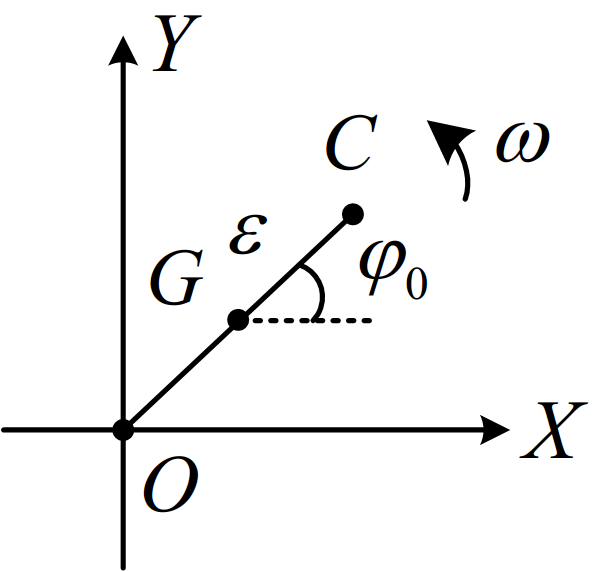
\includegraphics[scale=1.0]{4-geo_axis.png}
	\caption{圆盘静止时几何中心、质量中心、旋转中心和偏心距的分布}
	\label{fig:4-geo_axis}
\end{figure}
\autoref{fig:4-geo_axis}~显示了存在初始不平衡质量圆盘的偏心距的幅值和相位的示意图。转子在平面的运动轨迹可由位移信号$x(t)$和$y(t)$描述。考虑到$x(t)$和$y(t)$正交,转子运动轨迹可以用矢量$\boldsymbol{z}(t) = x(t) + jy(t)$来表示。同理,定义矢量$z_c(t)$、$z_g(t)$和$z_{\Delta}(t)$分别表示转子的质量中心、几何中心和偏心距的平面运动。那么
\begin{equation}
\boldsymbol{z}_c(t) = x_c(t) + jy_c(t)
\end{equation}
\begin{equation}
\boldsymbol{z}_g(t) = x_g(t) + jy_g(t)
\end{equation}
\begin{equation}
\label{eq:z_delta}
\boldsymbol{z}_{\Delta}(t) = \xi \cdot \cos(\omega t+\phi _0) + j\xi \cdot \sin(\omega t + \phi _0) = \xi e^{j(\omega t + \phi _0)}
\end{equation}
此三个矢量的关系为:
\begin{equation}
	\label{eq:z_c}
	\boldsymbol{z}_c(t) = \boldsymbol{z}_g(t) + \boldsymbol{z}_{\Delta}(t)
\end{equation}

零位移控制算法是指通过施加某些算法(如陷波器算法)消除转子位移振动,即使得旋转轴趋于几何轴。当圆盘的位移振动幅值被抑制到较低水平时,可将其几何中心与旋转中心视为重合,即
\begin{equation}
	\label{eq:z_g_0x}
	\boldsymbol{z}_g(t) = 0
\end{equation}
则此时偏心距分布如\autoref{fig:4-geo_axis_co}~所示。
\begin{figure}
	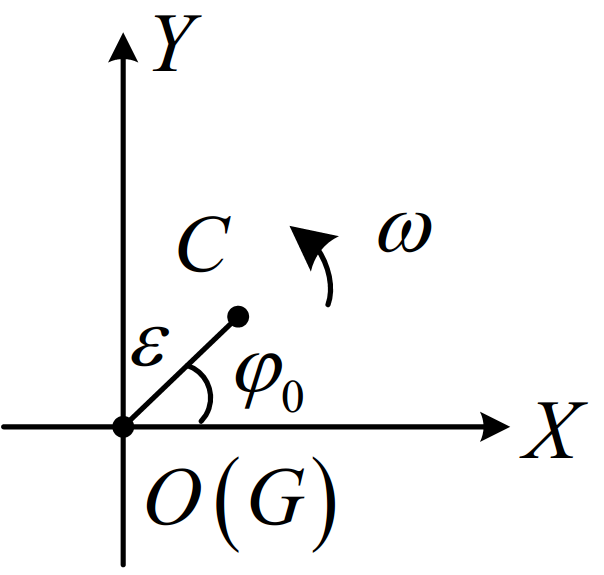
\includegraphics[scale=1.0]{4-geo_axis_co.png}
	\caption{几何中心与旋转中心重合时圆盘的偏心距分布}
	\label{fig:4-geo_axis_co}
\end{figure}

磁悬浮轴承中的磁悬浮力为:
\begin{equation}
	\label{eq:f_z}
	\boldsymbol{f}_z(t) = k_i \cdot \boldsymbol{i}_z(t) + k_s \cdot \boldsymbol{z}_g(t)
\end{equation}
研究圆盘的质心运动,可由牛顿第二运动定律得:
\begin{equation}
	\label{eq:f_z_a}
	\boldsymbol{f}_z(t) = m{\ddot{z}}_c(t)
\end{equation}
联立方程\autoref{eq:z_c}~、\autoref{eq:z_g_0x}~、\autoref{eq:f_z}~和\autoref{eq:f_z_a}~可得:
\begin{equation}
	\label{eq:geo_eq}
	-m \xi {\omega}^2e^{j(\omega t + \phi _0)} = k_ii_z(t)
\end{equation}
\autoref{eq:geo_eq}~显示了偏心距的幅值、相位与控制电流的关系。尽管偏心距的幅值和相位是不可直接测量的物理量,但是磁悬浮轴承中的控制电流是可以通过电流传感器测得的。因此,若记电流传感器测得的单端两自由度控制电流波形为
\begin{equation}
	\label{eq:i_z_0x}
	\boldsymbol{i}_z(t) = A_ie^{j(\omega t + \phi _i)}
\end{equation}
则将\autoref{eq:i_z_0x}~带入\autoref{eq:geo_eq}~可以解出偏心距的幅值和相位为
\begin{equation}
\left\{
\begin{aligned}
& \xi = \frac{k_iA_i}{m{\omega}^2}\\
& \phi _0 = \phi _i + \pi
\end{aligned}
\right.
\end{equation}


\subsection{零力法辨识转子偏心距}

零力法是指消除转子质量不平衡引起的磁悬浮振动力,使得$X$和$Y$方向磁悬浮力的交流分量均为零(直流分量需要提供负载所需的作用力,如重力,因此直流分量不一定为零)。当磁悬浮振动力被完全抑制时,转子旋转轴趋于惯性轴。当圆盘的磁悬浮振动力幅值被抑制到较低水平时,可将其惯性中心与旋转中心视为重合,即
\begin{equation}
	\label{eq:z_c_0f}
	\boldsymbol{z}_c(t) = 0
\end{equation}
此状态下偏心距的幅值和相位分布如\autoref{fig:4-ine_axis_co}~所示。将\autoref{eq:z_c_0f}带入\autoref{eq:z_c}中可以得到偏心距与几何中心的关系为:
\begin{equation}
	\label{eq:z_d_0f}
	\boldsymbol{z}_{\Delta}(t) = -\boldsymbol{z}_g(t)
\end{equation}
磁悬浮轴承中,转子的几何中心的位置可以通过位移传感器测得,由此可以求得偏心距的幅值和相位。此处记位移传感器测得的圆盘转子位移波形为:
\begin{equation}
	\label{eq:z_g_0f}
	\boldsymbol{z}_g(t) = A_ze^{j(\omega t + \phi _z)}
\end{equation}
联立\autoref{eq:z_d_0f}~和\autoref{eq:z_g_0f}~即可得到不平衡质量的幅值和相位为:
\begin{equation}
\left\{
\begin{aligned}
& \xi = A_z\\
& \phi _0 = \phi _z + \pi
\end{aligned}
\right.
\end{equation}

\begin{figure}[h!]
	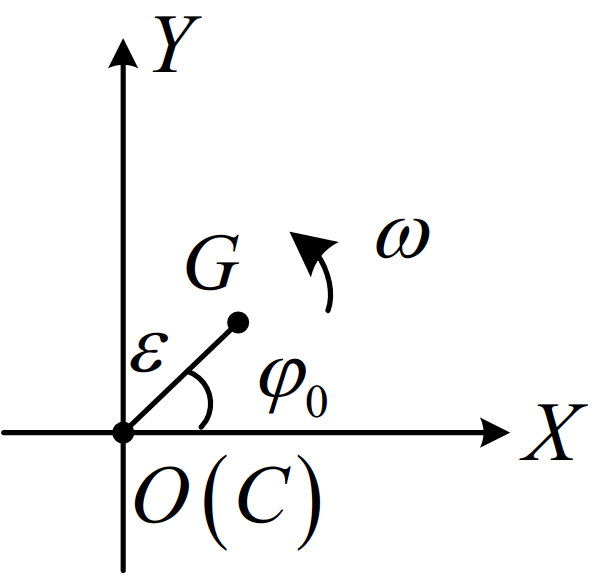
\includegraphics[scale=1.0]{4-ine_axis_co.png}
	\caption{质量中心与旋转中心重合时圆盘的偏心距分布}
	\label{fig:4-ine_axis_co}
\end{figure}


\subsection{零电流法辨识转子偏心距}

零电流控制是指消除控制电流中的同频分量,使得电流中的扰动信号的基波分量趋近于零(直流分量需要提供负载所需的作用力,如重力,因此直流分量不一定为零)。若不考虑传感器误差等引起的控制电流谐波分量,则控制电流可记为:
\begin{equation}
	\label{eq:i_z_0i}
	\boldsymbol{i}_z(t) = 0
\end{equation}
联立\autoref{eq:z_c}~、\autoref{eq:f_z}~和\autoref{eq:i_z_0i}~,可得
\begin{equation}
	\label{eq:0i_eq}
	m{\ddot{z}}_g(t) - m{\omega}^2\varepsilon e^{j (\omega t + \phi _0)} = k_sz_g(t) 
\end{equation}
可以看到,\autoref{eq:0i_eq}~中仅包含几何中心与偏心距,那么通过位移传感器测得圆盘几何中心的位移,即可推得偏心距的幅值和相位。\autoref{eq:0i_eq}~解得
\begin{equation}
	\label{eq:z_g_0i}
	A_z = \frac{\varepsilon}{1-\frac{k_s}{m{\omega}^2}}
\end{equation}
联立\autoref{eq:z_g_0f}~和\autoref{eq:z_g_0i}~,即可解出偏心距的幅值和相位为:
\begin{equation}
\label{eq:z_delta_0i}
\left\{
\begin{aligned}
& \xi = A_z\left( 1 -\frac{k_s}{m{\omega}^2} \right) \\
& \phi _0 = \phi _z
\end{aligned}
\right.
\end{equation}

通过以上的原理介绍可以看出,零位移法、零力法和零电流法均可以无需试重辨识出转子偏心距的分布。零位移法控制下转子振动位移降低,但是转子振动力加剧,适用于磁悬浮轴承定转子间气隙小、整机对振动力要求不严的场合;零力法和零电流法均可以显著抑制磁悬浮振动力,但是转子低速时转子位移振动加大,该方法适用于磁悬浮轴承定转子间气隙大、整机要求振动力小的场合。根据不同的应用场景,选择不同的方法来辨识偏心距分布,进而可据偏心距信息计算校正质量,实现转子不平衡质量校正(校正质量的计算和不平衡质量校正的详细方法见下一小节)。

\section{基于重复控制器的现场动平衡方法}

\subsection{零电流控制}

传统方案使用陷波器法实现零电流控制。陷波器是磁悬浮轴承振动抑制研究中应用较广的同频振动抑制策略,当其用于抑制电流中的同频振动成分以消除磁悬浮轴承振动力时,陷波器被以反馈的形式插入到闭环控制回路中。若以$N_f(s)$表示陷波器的开环传递函数,则插入陷波器的闭环系统控制框图如\autoref{fig:4-nfz}~所示。

\begin{figure}
	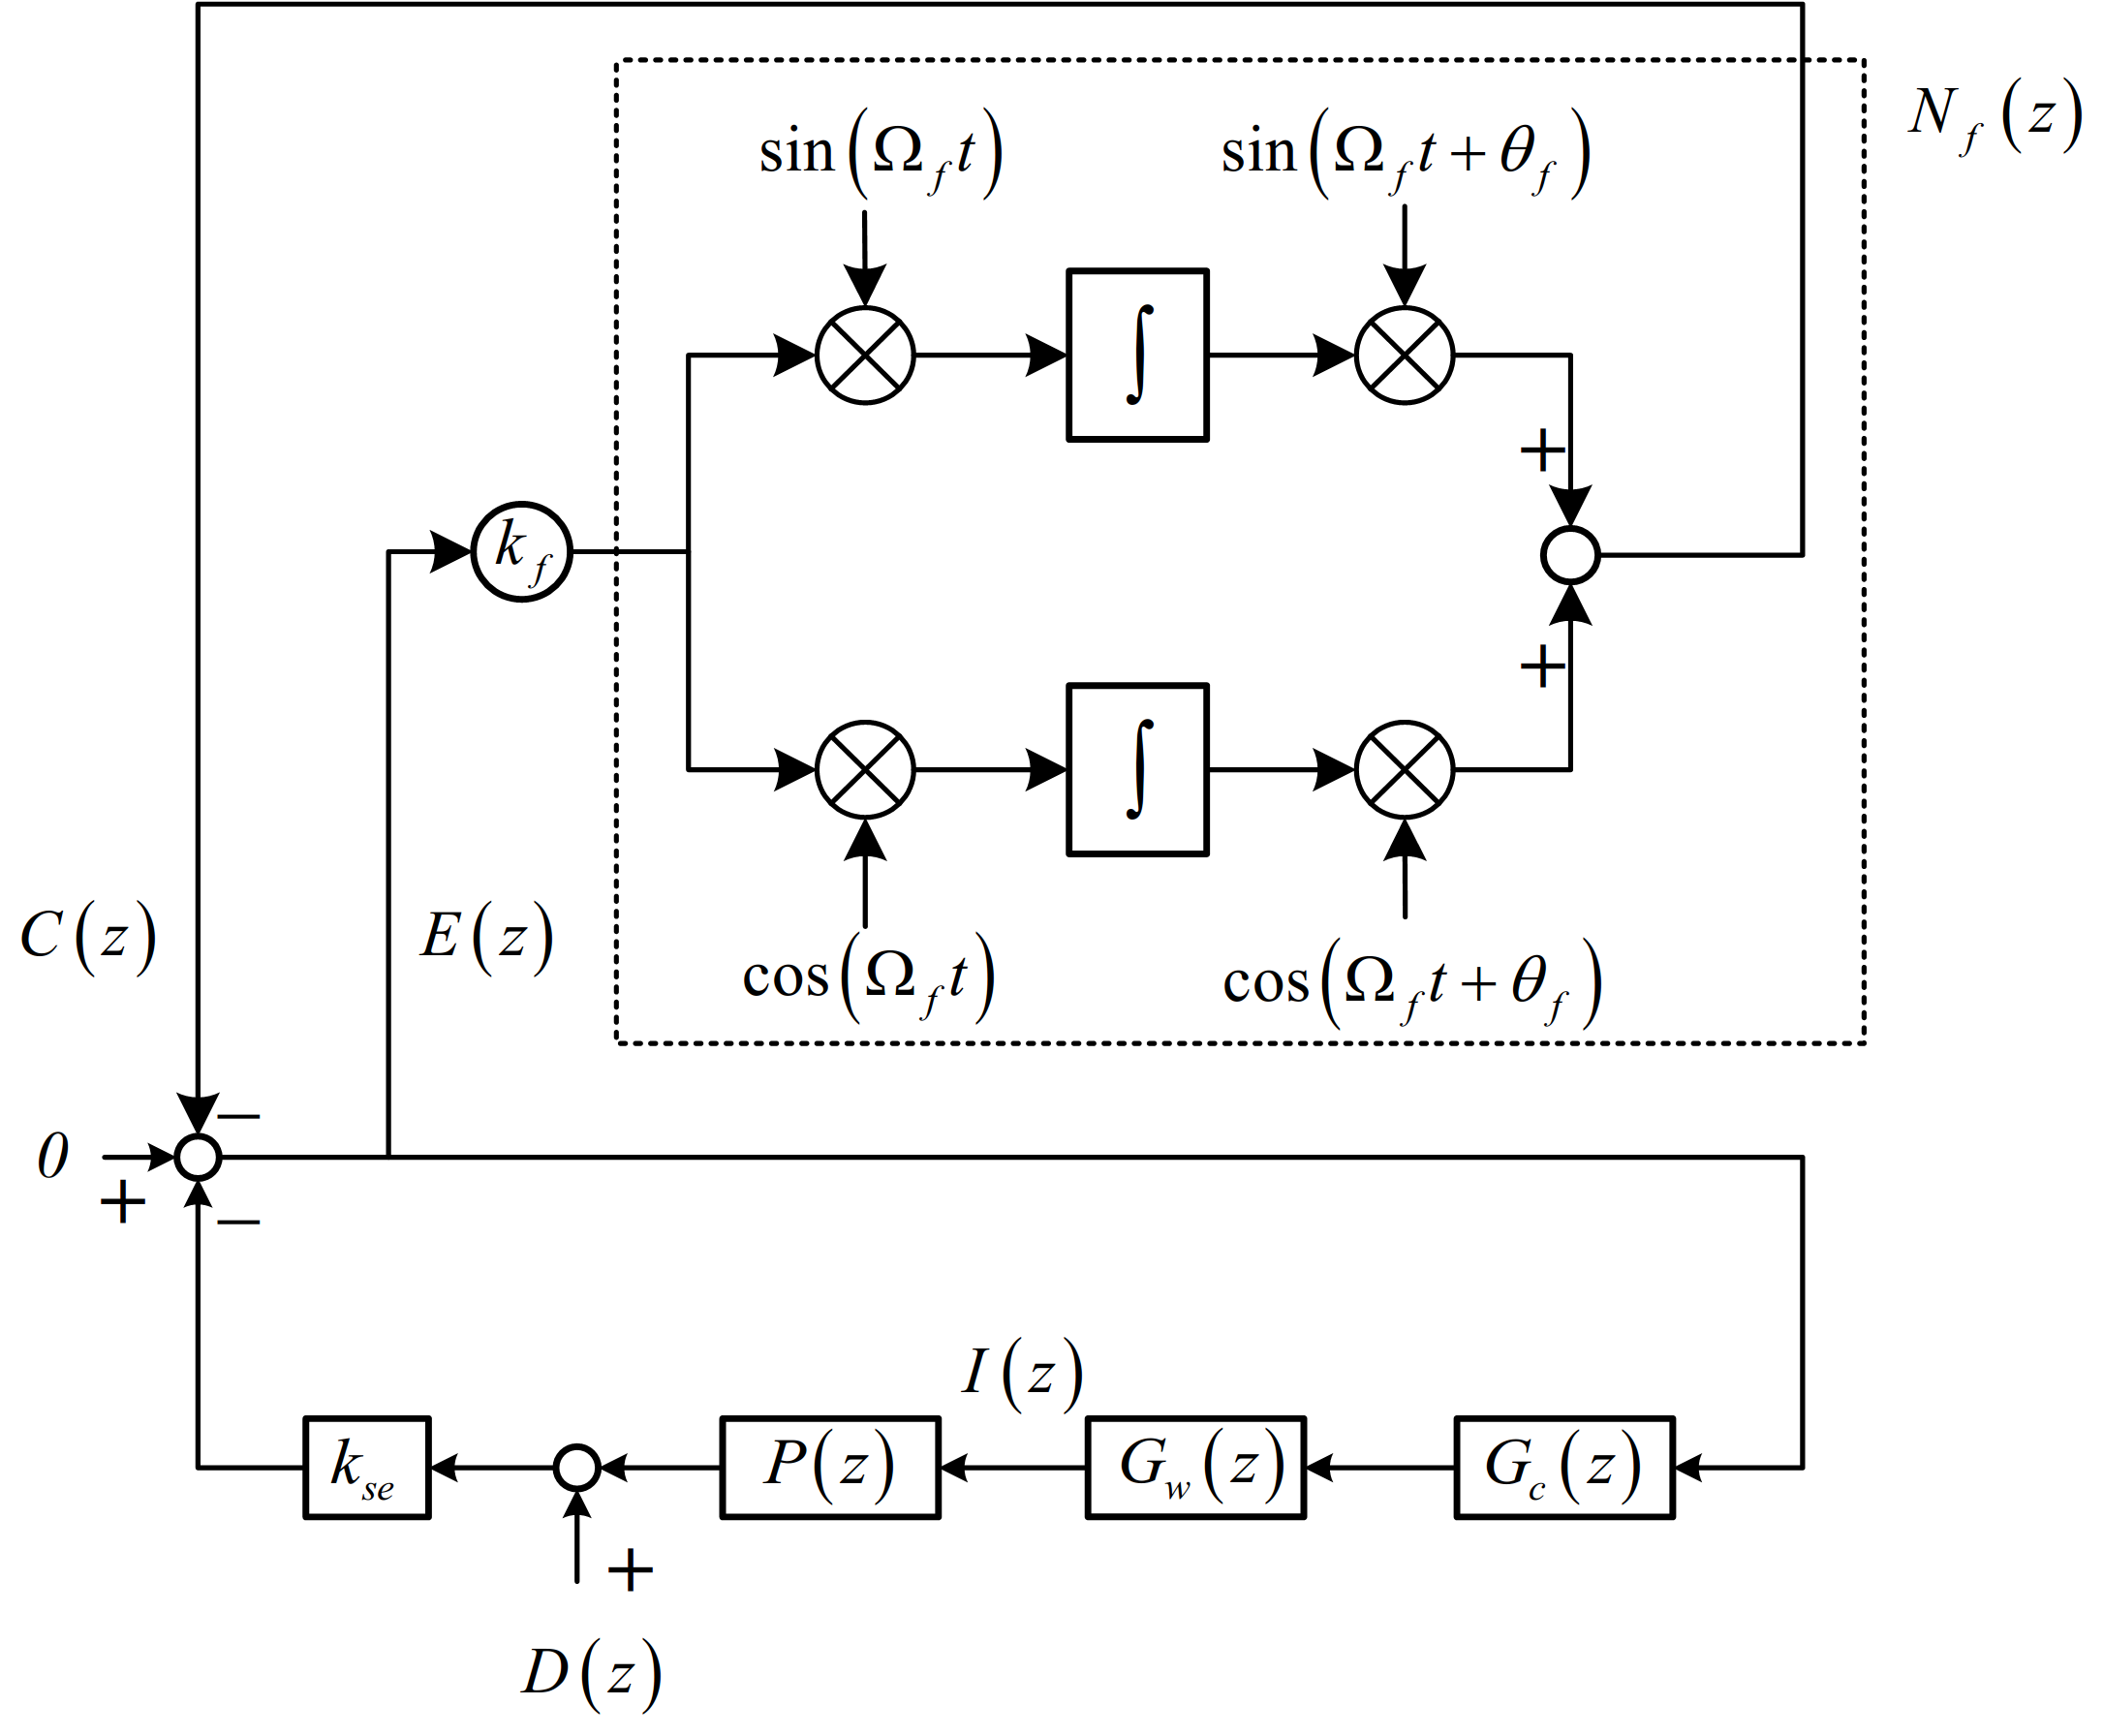
\includegraphics[scale=1.0]{4-nfz.png}
	\caption{插入陷波器的闭环系统控制框图}
	\label{fig:4-nfz}
\end{figure}

图中,$k_f$是指陷波器增益,$\theta _f$指陷波器相位角,$\Omega _f$是指陷波频率。为抑制同频振动力,此处陷波频率应选取为转子转动频率。陷波器的输入信号包括转子位移误差信号$e(t)$(对应图中$E(z)$)和一对相位相差$90^{\circ}$的正弦信号;陷波器的输出信号为$c(t)$(对应图中$C(z)$)。输入信号和输出信号的转换关系为:
\begin{equation}
c(t) = sin({\Omega}_f t + \theta _f) \int [sin({\Omega}_f t)e(t)]+cos({\Omega}_f t + \theta _f) \int [cos({\Omega}_f t)e(t)]
\end{equation}
上式两端同时以$t$为自变量求二次导数,可以得到
\begin{equation}
\ddot{c}(t) = -{{\Omega}_f}^2c(t)+cos(\theta _f)\dot{e}(t)-{\Omega}_f sin(\theta _f)e(t)
\end{equation}
对上式进行拉普拉斯变换得到:
\begin{equation}
s^2C(s) = -{{\Omega}_f}^2C(s)+scos(\theta _f)E(s)-{\Omega}_f sin(\theta _f)E(s)
\end{equation}
由此得到陷波器的开环传递函数$N_f(s)$为:
\begin{equation}
N_f(s) = \frac{C(s)}{E(s)} = \frac{scos(\theta _f) - {\Omega}_f sin(\theta _f)}{s^2 + {{\Omega}_f}^2}
\end{equation}
那么陷波器的闭环传递函数$N(s)$为:
\begin{equation}
N(s) = \frac{1}{1+k_fN_f(s)}=\frac{s^2+{{\Omega}_f}^2}{s^2+k_fcos(\theta _f)s + {{\Omega}_f}^2-k_f{\Omega}_f sin(\theta _f)}
\end{equation}

可以看出$N(s)$在$\omega = \Omega _f$处存在零点,所有在闭环系统稳定的条件下,加入该陷波器可以使同频电流的幅值完全消除。依据文献\cite{何家希2018磁悬浮高速电机主动振动控制方法及实验研究}给出的插入陷波器的闭环控制回路的稳定性分析方法,陷波器的参数$k_f$和$\theta _f$的选取原则为:

(1)$\theta _f = - arg\left[ S_0(j\Omega) \right]$,其中$S_0$为该自由度的输出敏感度函数;

(2)$k_f$越大,误差收敛速度越快,但是系统稳定性越差。实验过程中应该根据实验现象由小至大选取合适的$k_f$值。

新型方案使用ZORC实现零电流控制。位移传感器引入的谐波扰动使得控制电流中包含不仅包含质量不平衡引起的与转速同频的扰动,也包含谐波成分。使用传统的陷波器抑制同频振动电流后,其剩下的控制电流${i_t}$可以表示为:
\begin{equation}
	\label{eq:iz_0i_h}
	{i_t} = \sum\limits_{n = 2}^\infty  {{A_{ni}}{e^{j(n\omega t + {\varphi _{ni}})}}} 
\end{equation}
上式表明控制电流的交流分量并不为零。对于基于零电流控制的转子偏心距辨识方法而言,辨识结果准确度则无法保证。本文使用第三章提出的ZORC消除控制电流中的同频分量和谐波分量,实现零电流控制。对于同一磁悬浮轴承系统,基于ZORC的现场动平衡方法可复用第三章所述的ZORC控制结构及参数,无需另行设计。

\subsection{辨识偏心距}

考虑振动力的转子动力学方程为
\begin{equation}
\boldsymbol{M} \left( { \boldsymbol{{\ddot q}_g} + \boldsymbol{{{\ddot q}}_\Delta } } \right) + \boldsymbol{G}\left( { \boldsymbol{{\dot q}_{g}} + \boldsymbol{{{\dot q}}_\Delta } } \right) = \boldsymbol{B} \boldsymbol{K_s} {{\boldsymbol{B}}^{T}} \boldsymbol{{q}_g} + \boldsymbol{B} \boldsymbol{{K}_{i}} \boldsymbol{i}
\end{equation}
当控制电流的交流分量为零时,上式重写为
\begin{equation}
\boldsymbol{M}\left( {\boldsymbol{{\ddot q}_g} + {\boldsymbol{{\ddot q}}_\Delta }} \right) + \boldsymbol{G}\left( {\boldsymbol{{\dot q}_{g}} + \boldsymbol{{{\dot q}}_\Delta }} \right) = \boldsymbol{B}\boldsymbol{K_s}\boldsymbol{{B}^{T}}\boldsymbol{{q}_g}
\end{equation}
进行拉普拉斯变换后可得
\begin{equation}
\left( {\boldsymbol{M}{s^2} + \boldsymbol{G}s} \right)\left[ {\boldsymbol{q_g}\left( s \right) + \boldsymbol{q_\Delta }\left( s \right)} \right] =  \boldsymbol{B}\boldsymbol{{K}_{s}}{{\boldsymbol{B}}^{T}}\boldsymbol{{q}_g}\left( s \right)
\end{equation}
其中
\begin{equation}
\boldsymbol{B}\boldsymbol{K_s}{{\boldsymbol{B}}^{T}} = \left[ {\begin{matrix}
   \left({ l_{bA}^2 + l_{bB}^2} \right)k_s & { - {l_{bA}} + {l_{bB}}} & 0 & 0  \cr 
   { - {l_{bA}} + {l_{bB}}} & 2k_s & 0 & 0  \cr 
   0 & 0 & \left({ l_{bA}^2 + l_{bB}^2} \right)k_s & { - {l_{bA}} + {l_{bB}}}  \cr 
   0 & 0 & { - {l_{bA}} + {l_{bB}}} & 2k_s  \cr 
 \end{matrix} } \right]
\end{equation}
当两端磁极到中心距离一致,即${l_{bA}} = {l_{bB}} = {l_b}$时,上式可以化简为:
\begin{equation}
\label{eq:sys_b}
\boldsymbol{B}\boldsymbol{K_s}{{\boldsymbol{B}}^{T}} = \left[ {\begin{matrix}
   {2l_b^2k_s} & 0 & 0 & 0  \cr 
   0 & 2k_s & 0 & 0  \cr 
   0 & 0 & {2l_b^2k_s} & 0  \cr 
   0 & 0 & 0 & 2k_s  \cr 

 \end{matrix} } \right]
\end{equation}
转子径向上的运动分为平动和转动:$x$、$y$运动和$\alpha$、$\beta$运动。在\autoref{eq:sys_b}~所示的条件下,径向上的平动和转动可以解耦分析。定义复数信号$\boldsymbol{\eta} _g(t)$和$\boldsymbol{\nu} _g(t)$分别表示转子几何中心的平动位移和转动位移,复数信号$\boldsymbol{\eta} _{\Delta}(t)$和$\boldsymbol{\nu} _{\Delta}(t)$分别表示转子平动和转动方向上的偏心距,表示为:
\begin{equation}
\label{eq:decouple_define}
\left\{
\begin{aligned}
& \boldsymbol{\eta} _g(t) = x_g(t) + jy_g(t)\\
& \boldsymbol{\eta} _{\Delta}(t) = x_{\Delta}(t) + jy_{\Delta}(t)\\
& \boldsymbol{\nu} _g(t) = {\beta}_g(t) - j{\alpha}_g(t)\\
& \boldsymbol{\nu} _{\Delta}(t) = {\beta}_{\Delta}(t) - j{\alpha}_{\Delta}(t)\\
\end{aligned}
\right.
\end{equation}
根据\autoref{eq:q_delta}~定义,转子平动和转动方向上的偏心距分别为:
\begin{equation}
\label{eq:eta_nu_define}
\left\{
\begin{aligned}
&\boldsymbol{\eta} _{\Delta}(t) = ee^{j(\omega t + \theta)} \\
&\boldsymbol{\nu} _{\Delta}(t) = \sigma e^{j(\omega t + \gamma)} \\
\end{aligned}
\right.
\end{equation}
在不影响实际实验准确性的前提下,我们假设:

(1)转子径向对称:$I_x = I_y = I_r$;

(2)忽略细长转子的陀螺效应,即认为$\boldsymbol{G} = 0$

则\autoref{eq:sys_b}~和\autoref{eq:decouple_define}~可以重写为:
\begin{equation}
\label{eq:decouple}
\left\{
\begin{aligned}
& ms^2\left[ \boldsymbol{\eta} _g(s)+\boldsymbol{\eta}_{\Delta}(s) \right] = 2k_s\eta _g(s)\\
& {I_r}s^2\left[ \boldsymbol{\nu} _g(s)+\boldsymbol{\nu}_{\Delta}(s) \right] = 2k_s{l_b}^2\boldsymbol{\nu} _g(s)\\
\end{aligned}
\right.
\end{equation}
\autoref{eq:decouple}~可以解出:
\begin{equation}
\label{eq:cofficient}
\left\{
\begin{aligned}
& \boldsymbol{\eta} _g (t) = -\frac{m{\omega}^2}{m{\omega}^2+2k_s}\boldsymbol{\eta} _{\Delta}(t)\\
& \boldsymbol{\nu} _g (t) = -\frac{I_r{\omega}^2}{I_r{\omega}^2+2k_s{l_b}^2}\boldsymbol{\nu} _{\Delta}(t)\\
\end{aligned}
\right.
\end{equation}
由\autoref{eq:cofficient}~可以看出,得到$\boldsymbol{\eta} _g(t)$和$\boldsymbol{\nu} _g(t)$的信息才能得到不平衡质量的幅值和相位。但是如前文所提到,由于传感器误差的存在,转子几何中心无法测得。考虑到与质量不平衡引起的同频振动的幅值相比,传感器误差引起的同频振动的幅值要小得多,则不妨假设
\begin{equation}
\label{eq:assumption}
\left\{
\begin{aligned}
& \boldsymbol{\eta} _g (t) = \boldsymbol{\eta} _s (t)\\
& \boldsymbol{\nu} _g (t) = \boldsymbol{\nu} _s (t)  \\
\end{aligned}
\right.
\end{equation}
$\boldsymbol{\eta} _s(t)$和$\boldsymbol{\nu} _s(t)$可以通过位移传感器采集得到,其可以表示为
\begin{equation}
\label{eq:eta_s}
\left\{
\begin{aligned}
& \boldsymbol{\eta} _s (t) = A_{{\eta}}e^{j(\omega t + \phi _{\eta})} \\
& \boldsymbol{\nu} _s (t) = A_{{\nu}}e^{j(\omega t + \phi _{\nu})} \\
\end{aligned}
\right.
\end{equation}
联立\autoref{eq:eta_nu_define}~、\autoref{eq:cofficient}~和\autoref{eq:eta_s}~,可以解得偏心距的幅值和相位为:
\begin{equation}
\left\{
\begin{aligned}
& \xi = A_{\eta}\frac{m{\omega}^2 + 2k_s}{m{\omega}^2}\\
& \sigma = A_{\nu}\frac{I_r{\omega}^2 + 2k_s{l_b}^2}{I_r{\omega}^2}\\
\end{aligned}
\right.
\end{equation}
通过转角传感器辨识双端位移波形相位,即可获取平动和转动方向的偏心距的初相位$\theta$和$\gamma$。

\subsection{计算校正质量}

辨识出偏心距的幅值和相位之后,通过在双端配重盘增重的方式来校正转子初始不平衡质量。记在校正盘A上的校正质量为$m_A$,相位为$\phi _A$;校正盘B上的校正质量为$m_B$,相位为$\phi _B$。则校正力矩矩阵可以表示为:
\begin{equation}
\boldsymbol{Q_c} = \boldsymbol{T_c} \cdot \boldsymbol{M_c}
\end{equation}
其中
\begin{equation}
\boldsymbol{M_c}{\rm{ = }}\left[ {\begin{matrix}
   {{m_a}{r_a}\cos \left( {{\varphi _A}} \right)}  \cr 
   {{m_b}{r_b}\cos \left( {{\varphi _B}} \right)}  \cr 
   {{m_a}{r_a}\sin \left( {{\varphi _A}} \right)}  \cr 
   {{m_b}{r_b}\sin \left( {{\varphi _B}} \right)}  \cr 

 \end{matrix} } \right]
\end{equation}
\begin{equation}
\boldsymbol{T_c} = \left[ {\begin{matrix}
   { - {l_{cA}}} & {{l_{cB}}} & 0 & 0  \cr 
   1 & 1 & 0 & 0  \cr 
   0 & 0 & { - {l_{cA}}} & {{l_{cB}}}  \cr 
   0 & 0 & 1 & 1  \cr 

 \end{matrix} } \right]
\end{equation}
校正目标为转子合力矩为零,即
\begin{equation}
\label{eq:com_tar}
\boldsymbol{M}\boldsymbol{q_{\Delta}}{\omega}^2 + \boldsymbol{Q_c}\boldsymbol{T_c}{\omega}^2 = 0
\end{equation}
解\autoref{eq:com_tar}~时,先令校正质量分布于正交方向$x$和$y$上,表示为
\begin{equation}
{\boldsymbol{M_c}}{\rm{ = }}\left[ {\begin{matrix}
   {{m_{ax}}{r_a}}  \cr 
   {{m_{bx}}{r_b}}  \cr 
   {{m_{ay}}{r_a}}  \cr 
   {{m_{by}}{r_b}}  \cr 

 \end{matrix} } \right]
\end{equation}
求出$\boldsymbol{T_c}$的逆矩阵为:
\begin{equation}
{\boldsymbol{T_c}}^{ - 1} = {1 \over {{l_{cA}} + {l_{cB}}}}\left[ {\begin{matrix}
   { - 1} & {{l_{cB}}} & 0 & 0  \cr 
   1 & {{l_{cA}}} & 0 & 0  \cr 
   0 & 0 & { - 1} & {{l_{cB}}}  \cr 
   0 & 0 & 1 & {{l_{cA}}}  \cr 

 \end{matrix} } \right]
\end{equation}
则可以解出正交方向上的校正质量为:
\begin{equation}
\left[ {\begin{matrix}
   {{m_{ax}}}  \cr 
   {{m_{bx}}}  \cr 
   {{m_{ay}}}  \cr 
   {{m_{by}}}  \cr 

 \end{matrix} } \right] =  - {1 \over {{l_{cA}} + {l_{cB}}}}\left[ {\begin{matrix}
   { - 1} & {{l_{cB}}} & 0 & 0  \cr 
   1 & {{l_{cA}}} & 0 & 0  \cr 
   0 & 0 & { - 1} & {{l_{cB}}}  \cr 
   0 & 0 & 1 & {{l_{cA}}}  \cr 

 \end{matrix} } \right]\left[ {\begin{matrix}
   {{I_r}\sigma \cos \gamma }  \cr 
   {m\varepsilon \cos \theta }  \cr 
   {{I_r}\sigma \sin \gamma }  \cr 
   {m\varepsilon \sin \theta }  \cr 

 \end{matrix} } \right]{\left[ {\begin{matrix}
   {{r_a}}  \cr 
   {{r_b}}  \cr 
   {{r_a}}  \cr 
   {{r_b}}  \cr 

 \end{matrix} } \right]^{ - 1}}
\end{equation}
得到校正质量幅值和相位为:
\begin{equation}
\left\{
\begin{aligned}
&{m_a} = \sqrt {m_{ax}^2 + m_{ay}^2}\\
&{m_b} = \sqrt {m_{bx}^2 + m_{by}^2} \\  
&{\varphi _A} = \arctan {{{m_{ay}}} \over {{m_{ax}}}} \\
&{\varphi _B} = \arctan {{{m_{by}}} \over {{m_{bx}}}} \\ 
\end{aligned}
\right.
\end{equation}


\section{实验分析}

在进行本节的分析与实验前,实验样机已在动平衡机上完成去重式转子动平衡,残余不平衡质量较小,250Hz运转时磁悬浮轴承位移波形如\autoref{fig:5-s3-x-w0-pid}~所示,径向自由度位移振动幅值仅约$10\mu m$。为测试验证本文提出的基于ZORC的现场动平衡方法的实际效果,本文在转子两端分别增加一定质量的配重以增大位移振动幅值、显示实验效果,增重之后250Hz运转时磁悬浮轴承位移波形如\autoref{fig:5-s3-x-w1-pid}~所示,径向自由度位移振动幅值约$20\mu m$。以此增重后的状态作为转子初始质量不平衡状态,再使用本文提出的基于谐波抑制的现场动平衡方法辨识该不平衡质量,并通过增重的方式进行校正,分析现场动平衡前后转子振动量级,以验证现场动平衡算法实际效果。

\begin{figure}[h!]  
	\subfloat[初始不平衡质量引起的位移振动\label{fig:5-s3-x-w0-pid}]{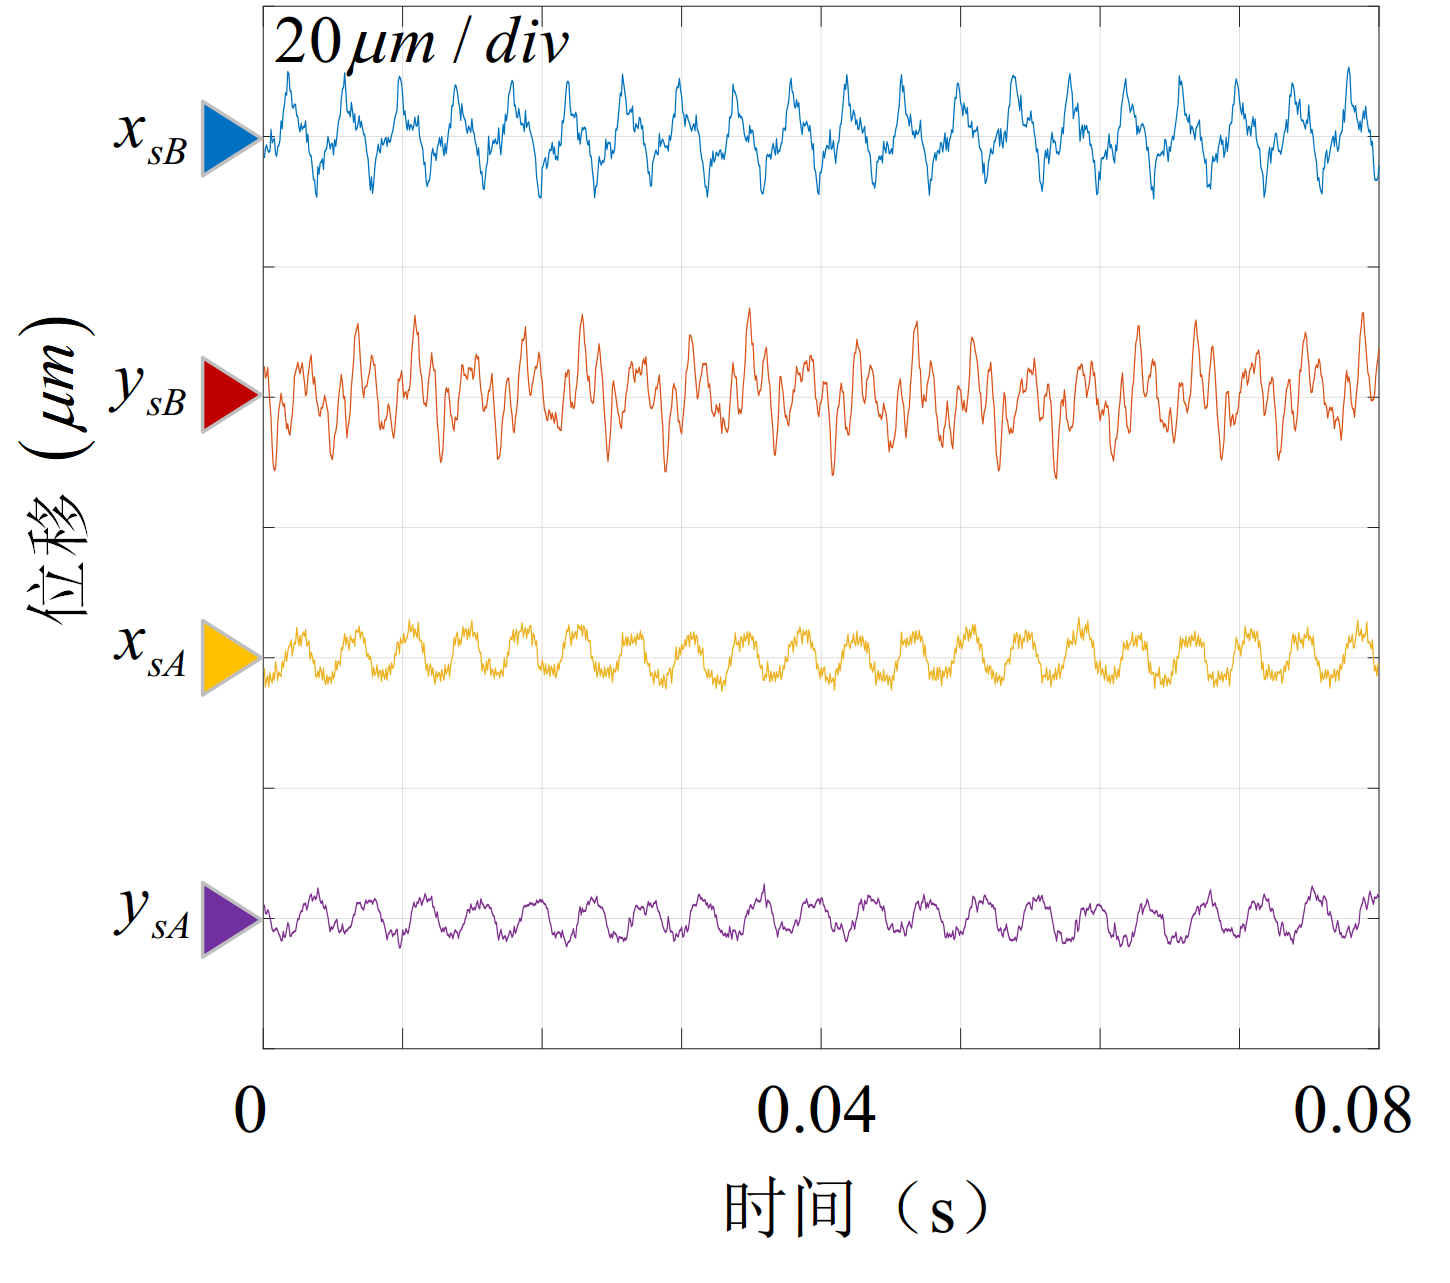
\includegraphics[scale=1.0]{5-s3-x-w0-pid.png}}\quad  
	\subfloat[增重后转子不平衡质量引起的位移振动\label{fig:5-s3-x-w1-pid}]{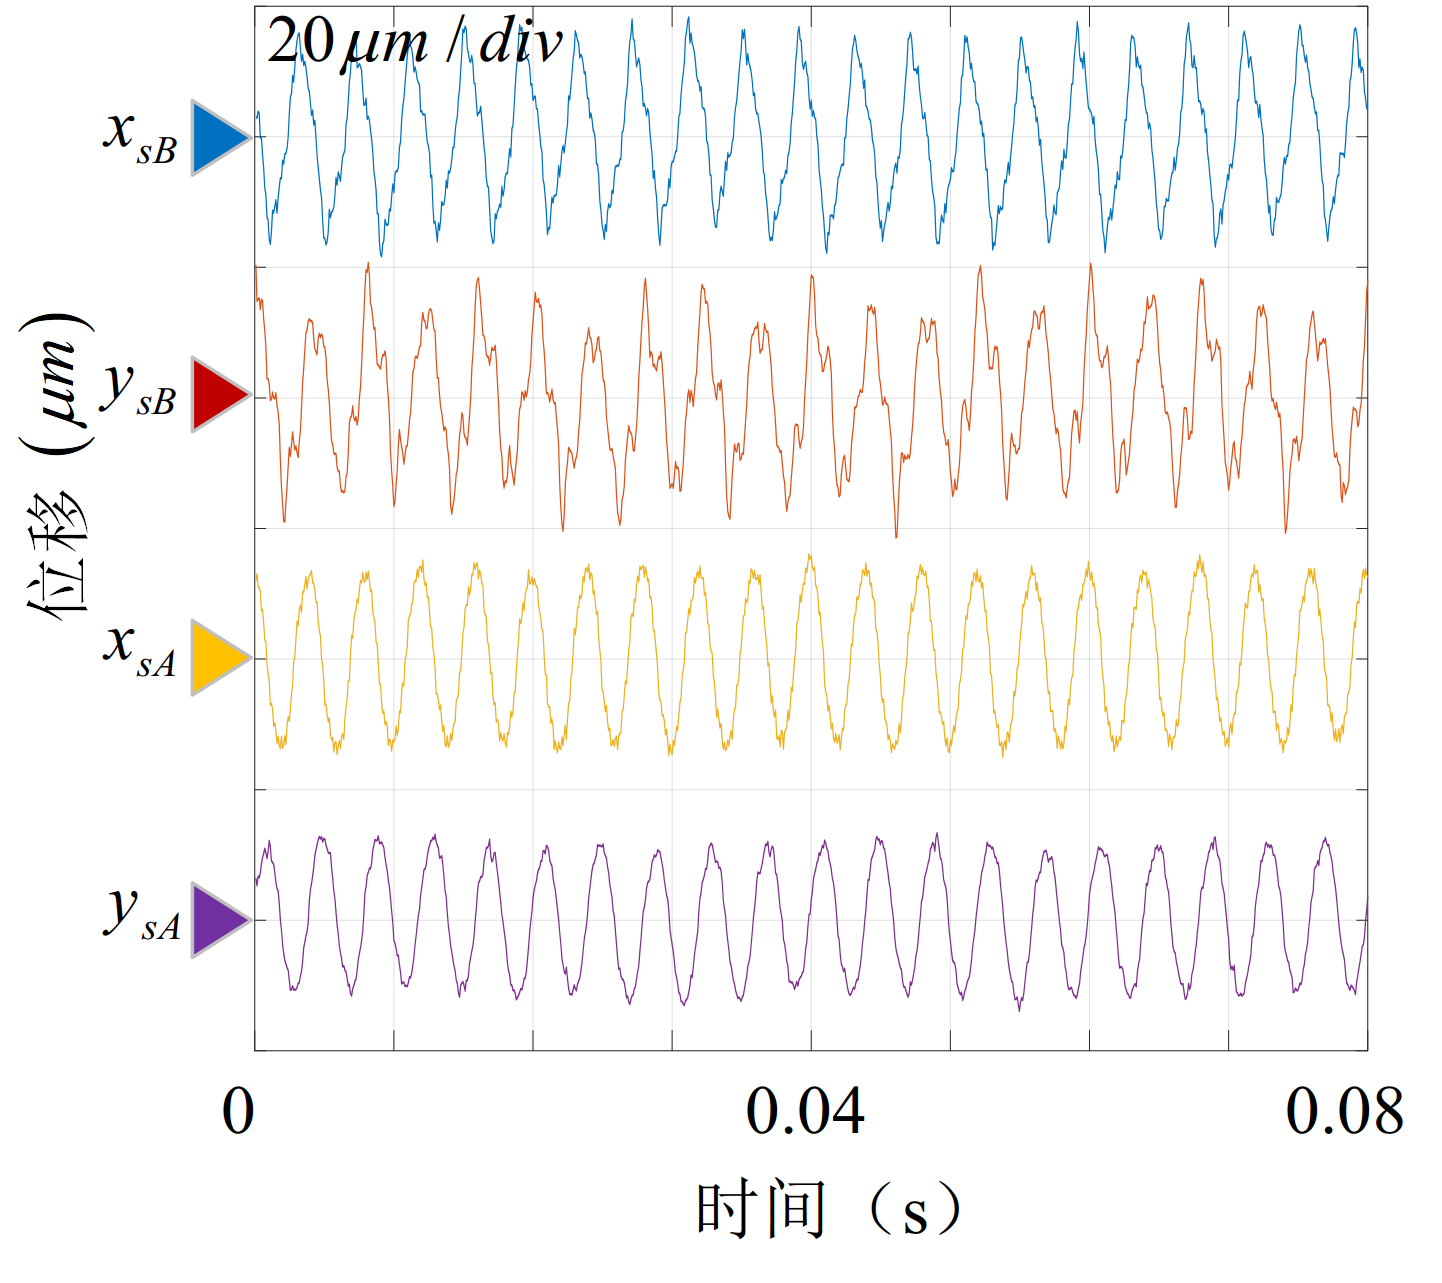
\includegraphics[scale=1.0]{5-s3-x-w1-pid.png}}  		\caption{转子不平衡质量引起的位移振动}  \label{fig:5-s3-x-w0/w1}\end{figure}
	
两端的配重盘尺寸一致,靠近边沿处沿圆形轨迹分布36个螺丝孔,每两个孔之间间距为$10^{\circ}$。每个孔上可以通过螺丝固定数量不等的垫片在配重盘上,达到增重的目的。增加初始配重质量的幅值和相位分别如\autoref{tab:nf_orc_w1}~所示。

首先分析传统零电流控制方案的效果。根据\autoref{fig:5-sens_x}~、\autoref{fig:5-sens_y}~、\autoref{fig:5-sens_u}~和\autoref{fig:5-sens_v}~所示的输出敏感度函数,转子在70Hz$\sim$100Hz附近增益幅值最大,则在该频率段转子的稳定性能较差。考虑转子到高速时各自由度输出敏感度增益较小,且相位变化平缓,因此本文选取250Hz作为位移波形采集点:将转子升速至250Hz,加入零电流控制算法后采集位移波形,辨识转子不平衡质量分布。从输出敏感度函数曲线上获取250Hz处的XA、XB、YA和YB通道的输出敏感度相位并设计陷波器参数$\theta _f$如\autoref{tab:250_S0_phase}~所示;陷波器参数$k_f$的选取步骤为:根据实验现象,从零逐渐增加陷波器参数$k_f$,当$k_f = 50$时,陷波器的同频振动振动抑制效果良好,因此选择$k_f = 50$。

\begin{table}[h!]
  \caption[径向各自由度在250Hz的输出敏感度相位]{径向各自由度在250Hz的输出敏感度相位\label{tab:250_S0_phase}}
  \begin{tabular}{ccc}
    \toprule
    自由度 & 250Hz处输出敏感度函数相位 & $\theta _f$ \\
    \midrule
    $X_A$ & $0^{\circ}$ & $0^{\circ}$\\
    $Y_A$ & $1^{\circ}$ & $-1^{\circ}$\\
    $X_B$ & $2^{\circ}$ & $-2^{\circ}$\\
    $Y_B$ & $0^{\circ}$ & $0^{\circ}$\\
    \bottomrule
  \end{tabular}
\end{table}

\begin{figure}[h!]  
	\subfloat[PID控制下控制电流时域波形\label{fig:5-s3-i-w1-pid}]{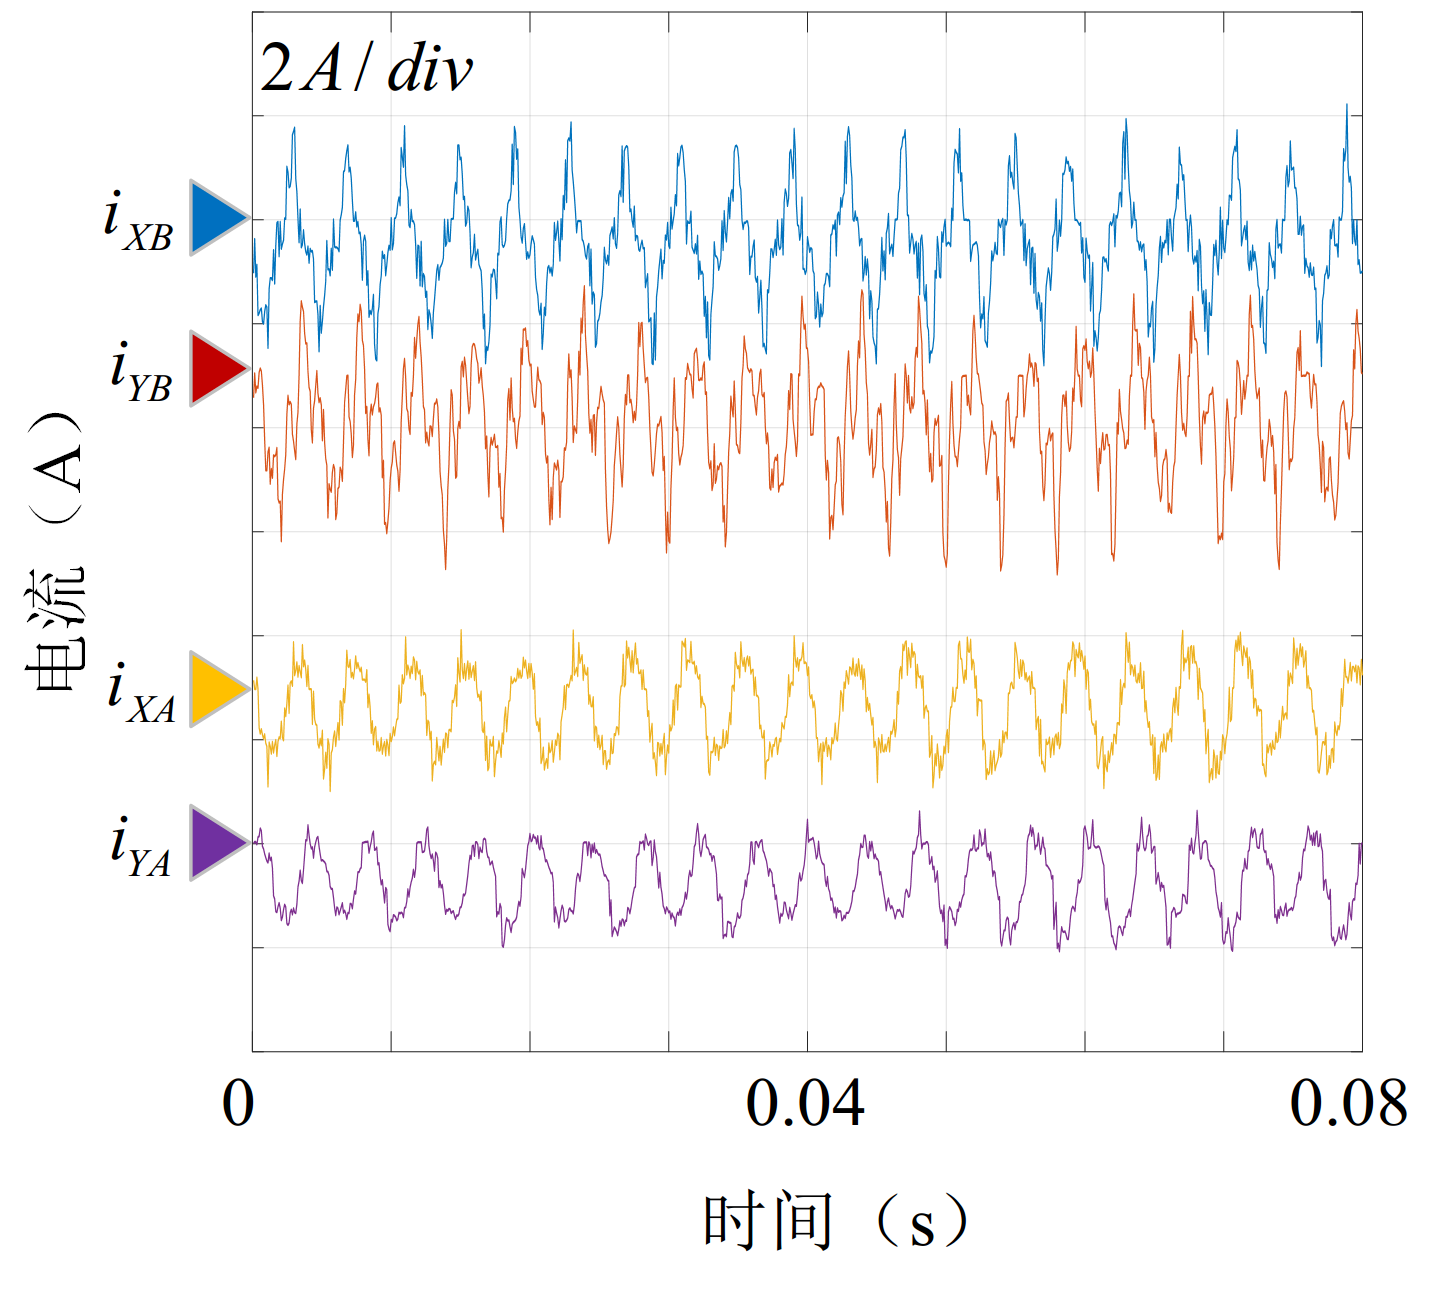
\includegraphics[scale=1.0]{5-s3-i-w1-pid.png}}\quad  
	\subfloat[PID+陷波器控制下控制电流时域波形\label{fig:5-s3-i-w1-pid-nf}]{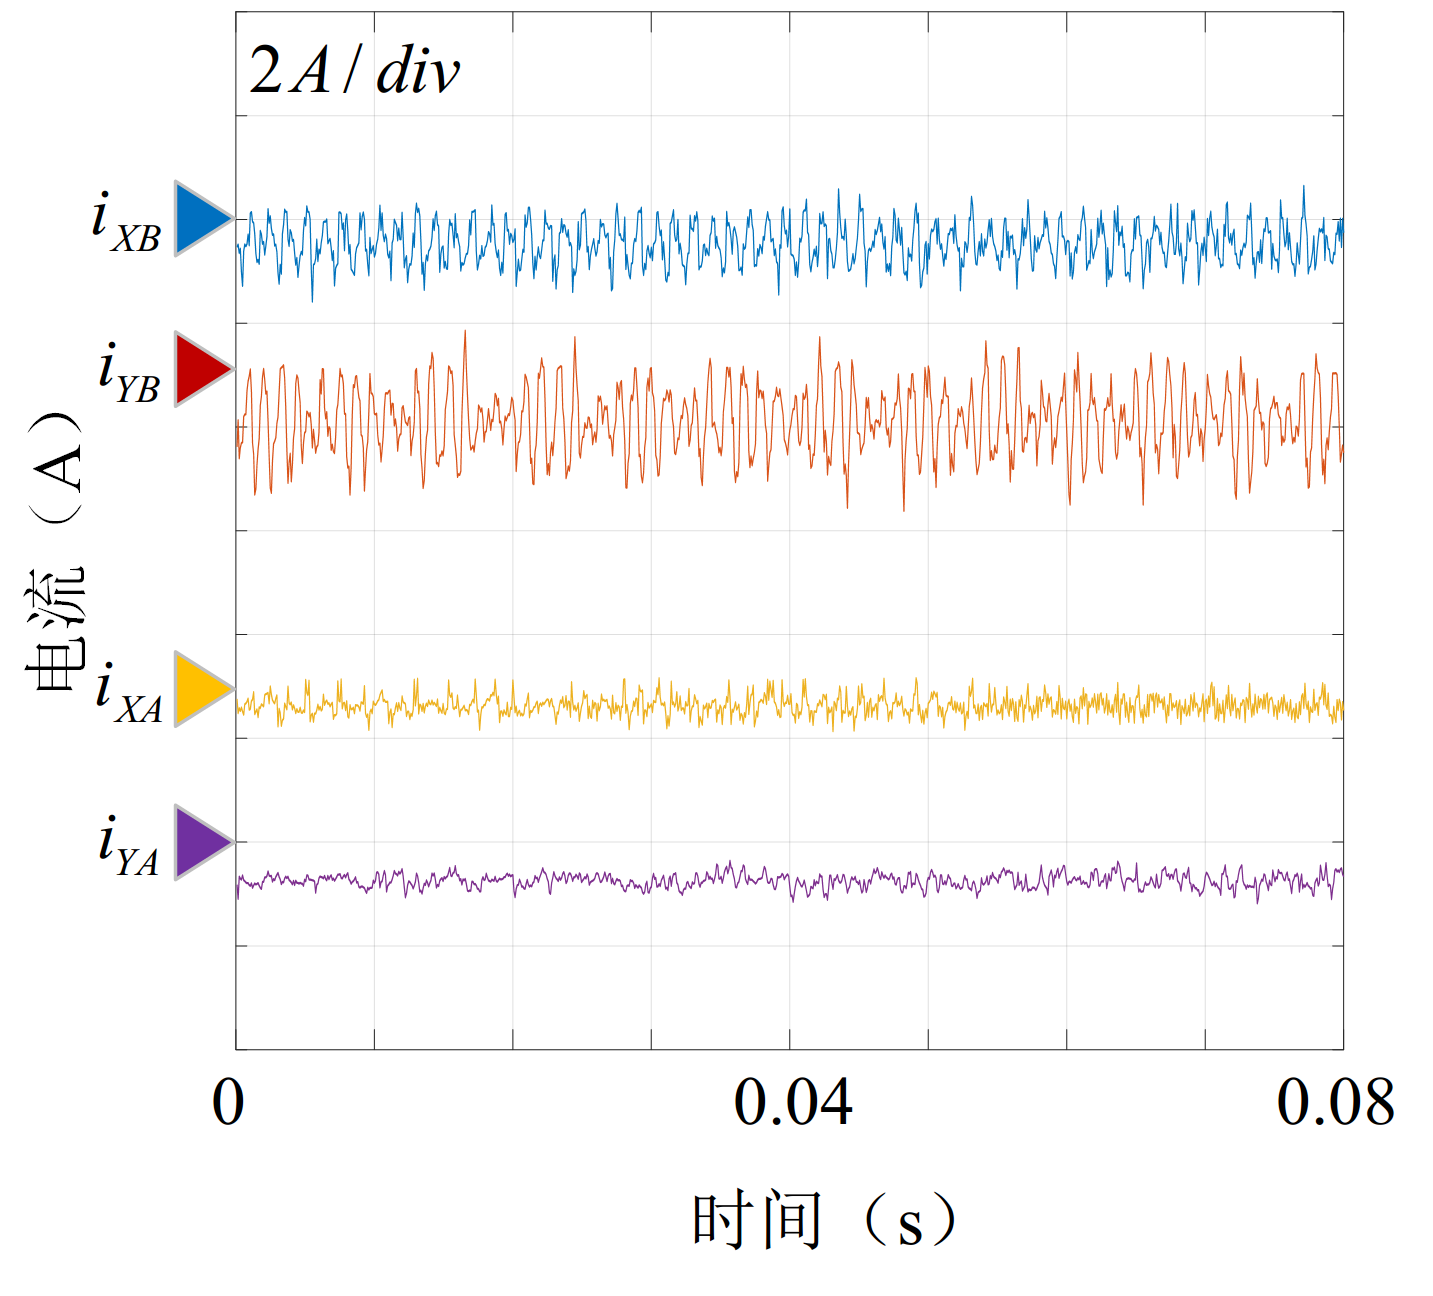
\includegraphics[scale=1.0]{5-s3-i-w1-pid-nf.png}}  
	\caption{加入陷波器前后控制电流时域波形}  \label{fig:5-s3-i-w1-pid_nf}\end{figure}
	
\begin{figure}[h!]
	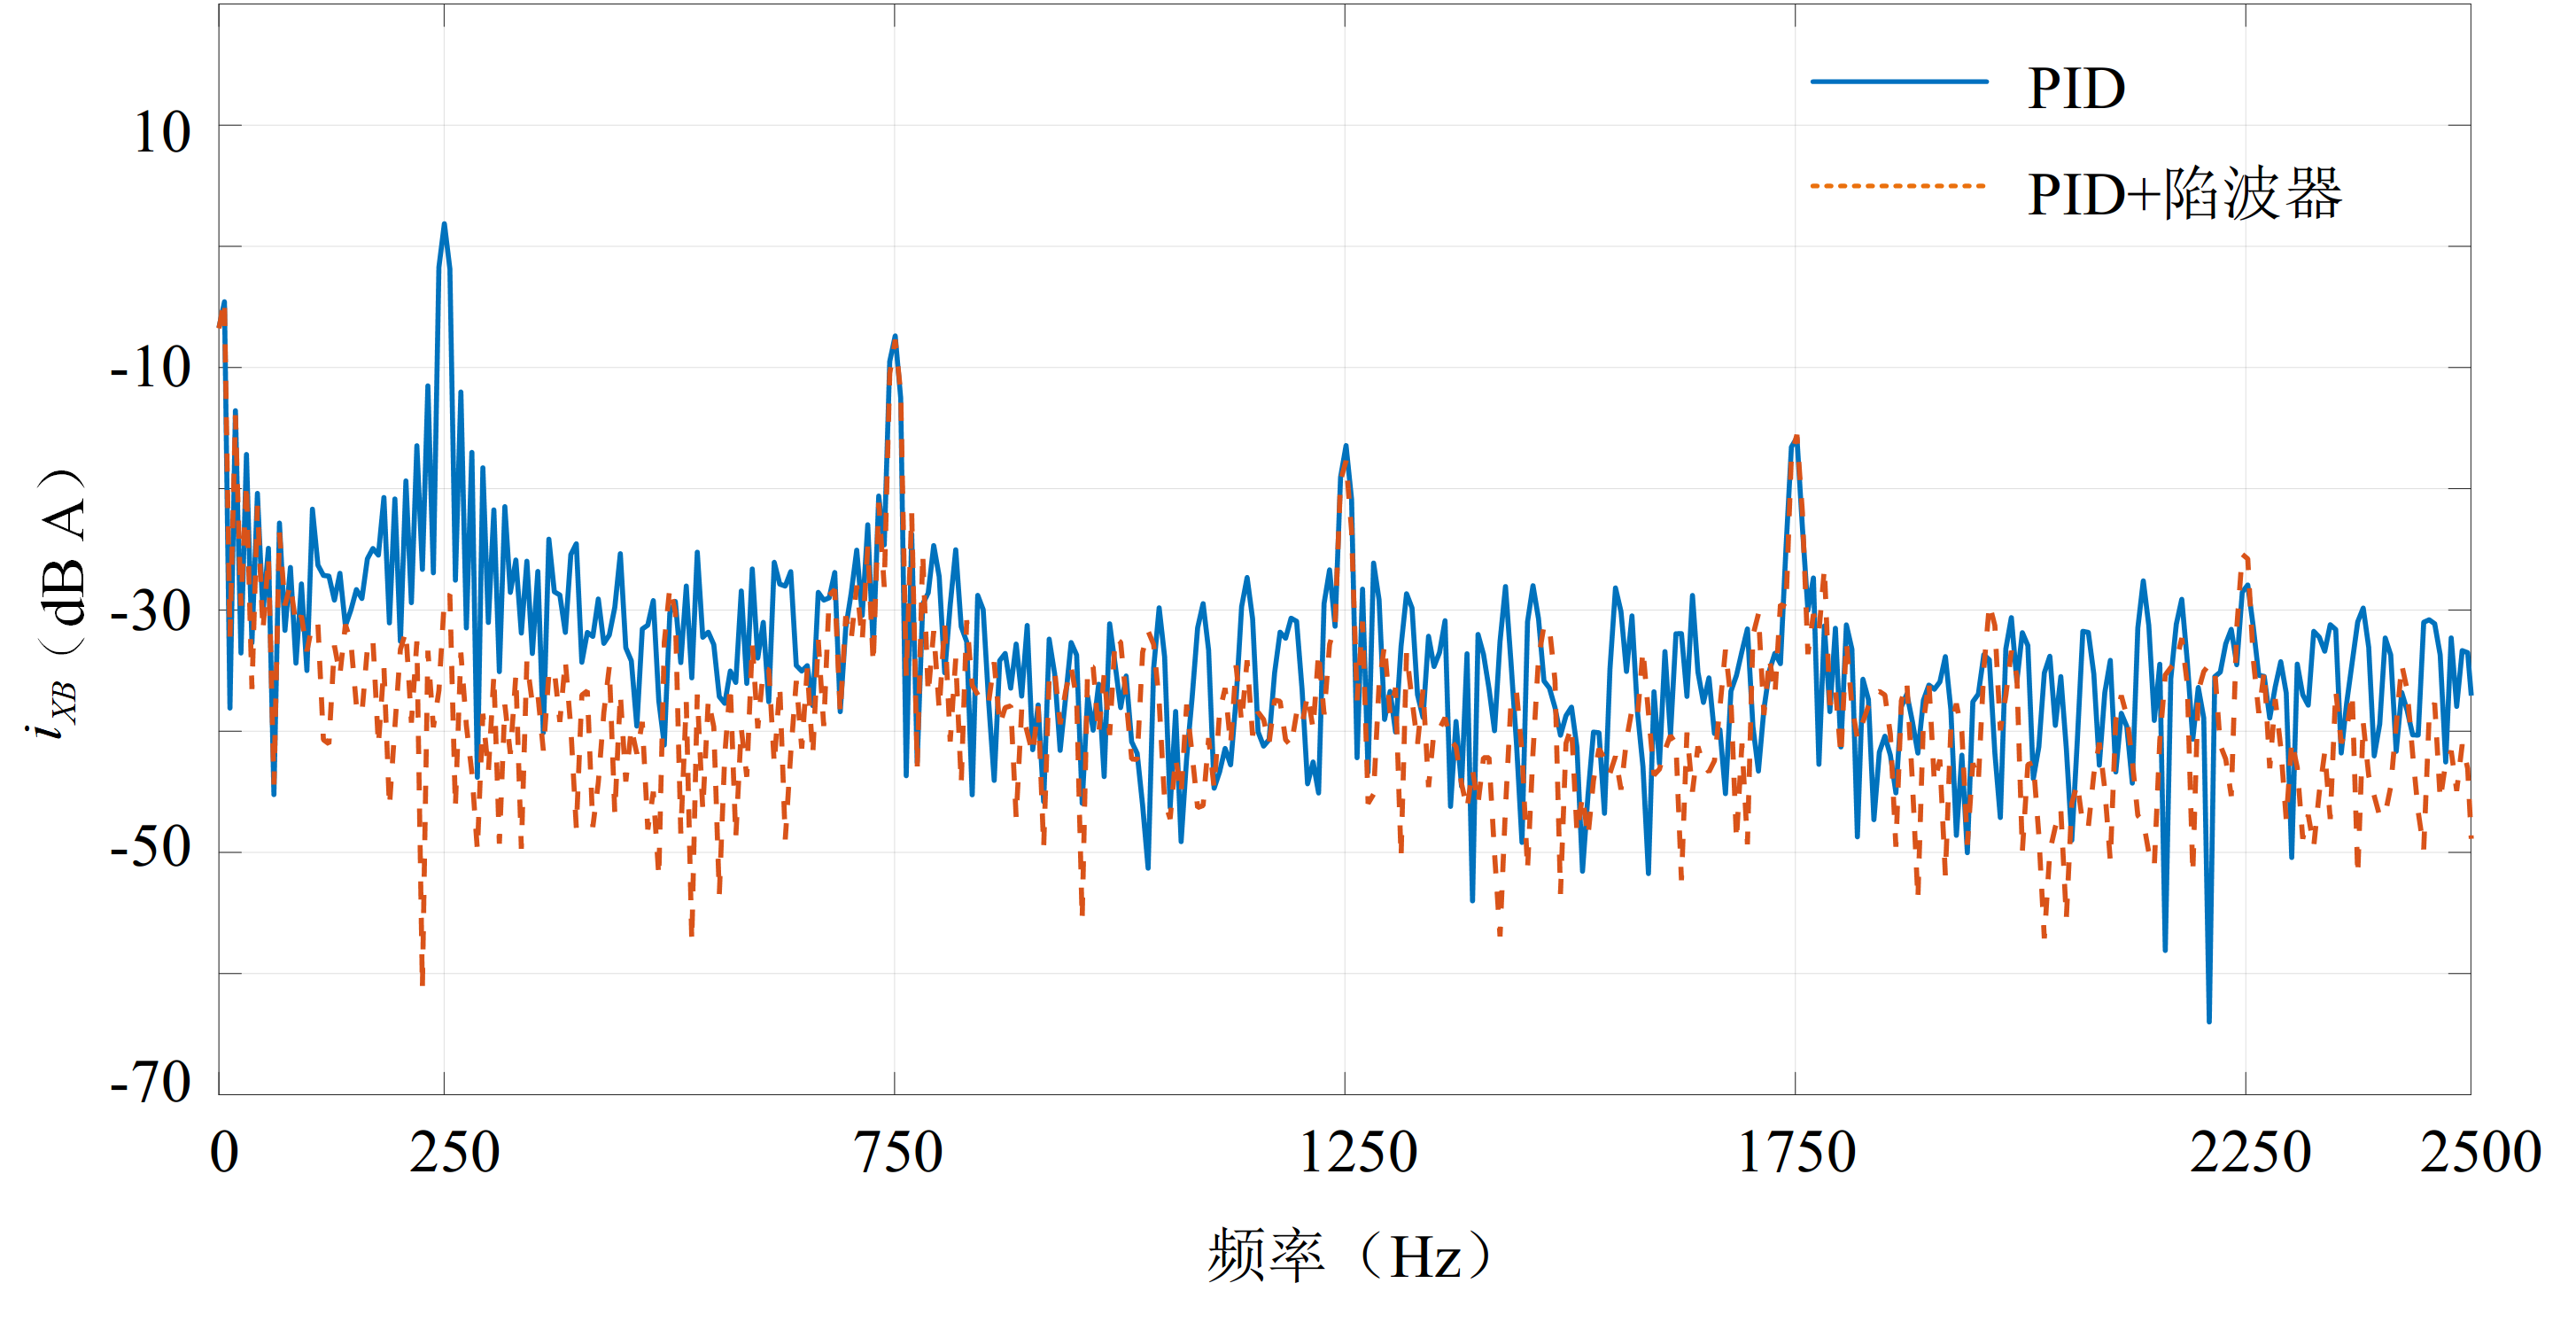
\includegraphics[scale=1.0]{5-s3-i_f-w1-pid_nf.png}
	\caption{加入陷波器前后$i_{XB}$频谱}
	\label{fig:5-s3-i_f-w1-pid_nf}
\end{figure}

\autoref{fig:5-s3-i-w1-pid_nf}~显示了加入陷波器前后控制电流时域波形。考虑到四个径向通道控制策略和控制对象模型一致,因此仅分析其中一个自由度的电流的频谱图像即可反应加入陷波器对控制电流的影响,此处不妨选取$i_{xB}$电流分析。\autoref{fig:5-s3-i-w1-pid}~显示了质量不平衡引起的控制电流振动,各自由度的控制电流幅值均较大,约1A$\sim$2A。从\autoref{fig:5-s3-i-w1-pid-nf}~可以看出,加入陷波器之后控制电流幅值明显衰减,降低至0.2A$\sim$1A。为了分析控制电流中各次谐波幅值的变化,对$i_{xB}$电流时域波形进行傅里叶分解,\autoref{fig:5-s3-i_f-w1-pid_nf}~显示了加入陷波器前后$i_{XB}$频谱。从图中可以看到控制电流中包含一、三、五和七次谐波,加入陷波器可以有效抑制同频振动电流:同频电流幅值从约-5dB A下降到约-30dB A,但是三、五和七次谐波的幅值并未显示任何衰减。该实验结果与理论是一致的,加入陷波器仅能有效抑制控制电流中的同频振动。

\begin{figure}[h!]  
	\subfloat[PID控制下控制电流时域波形\label{fig:5-s3-i-w1-pid_1}]{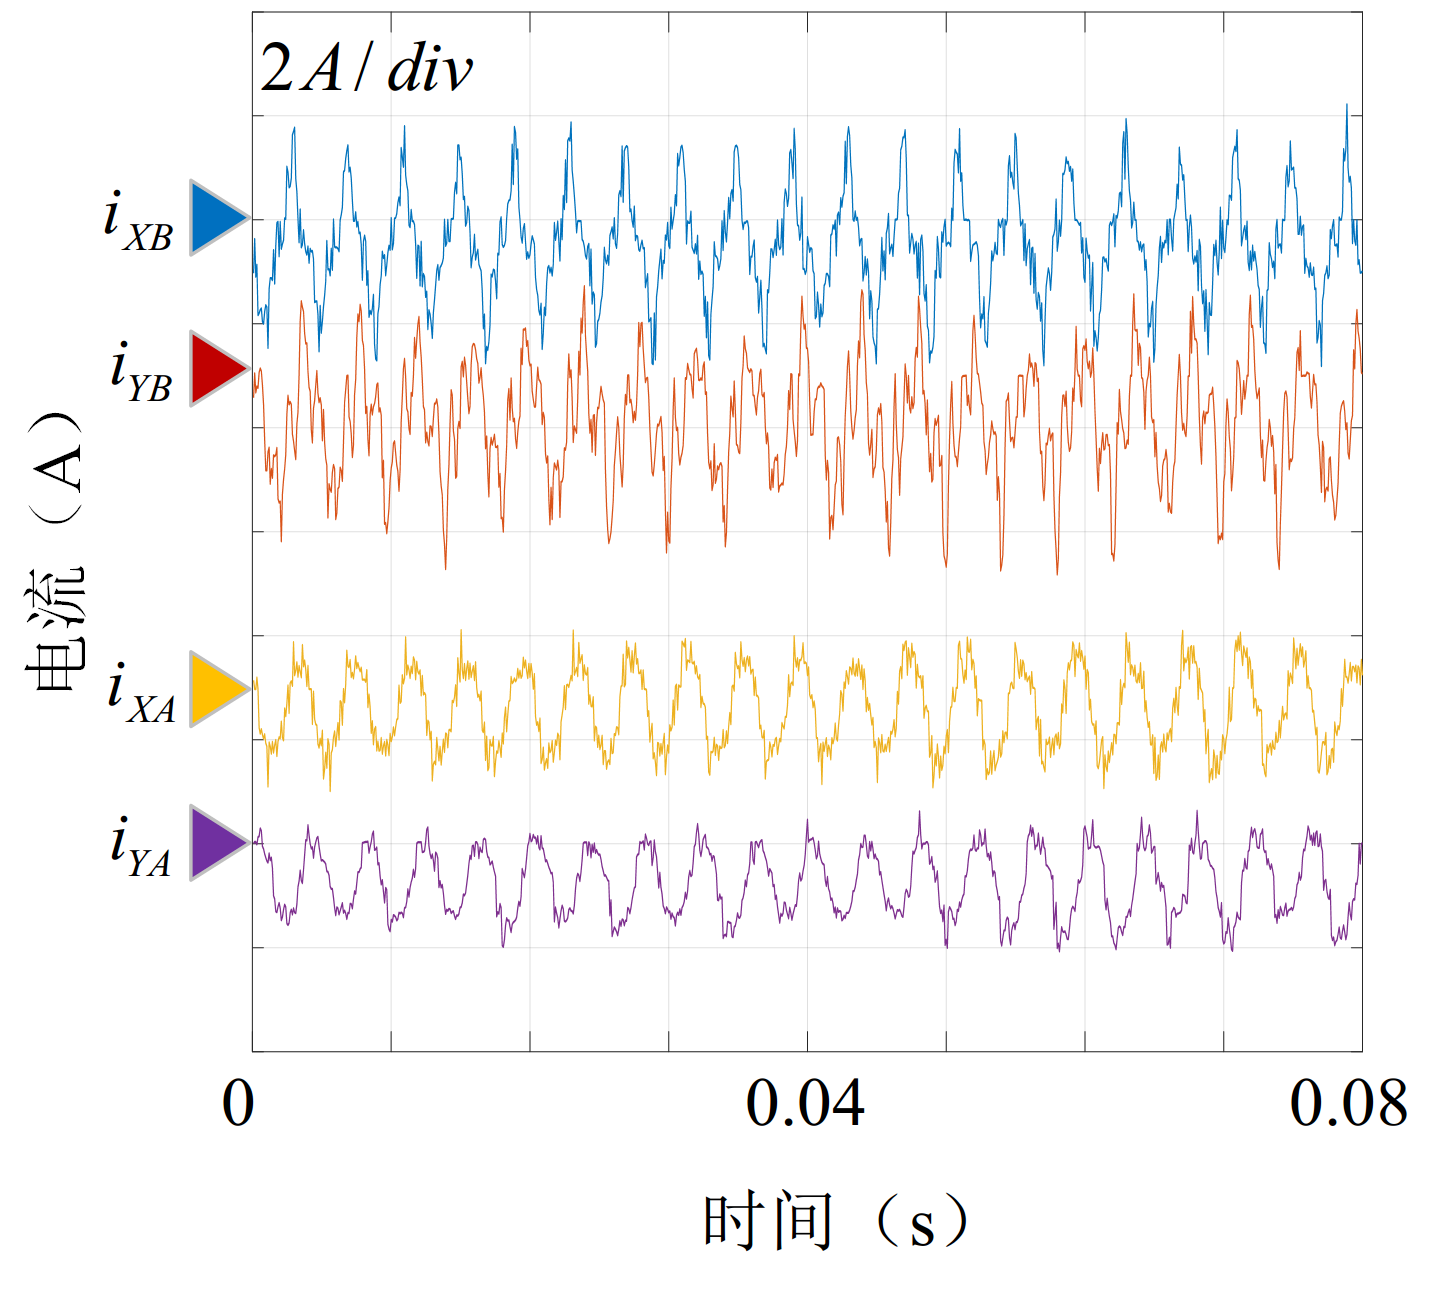
\includegraphics[scale=1.0]{5-s3-i-w1-pid.png}}\quad  
	\subfloat[PID+重复控制器控制下控制电流时域波形\label{fig:5-s3-i-w1-pid-orc}]{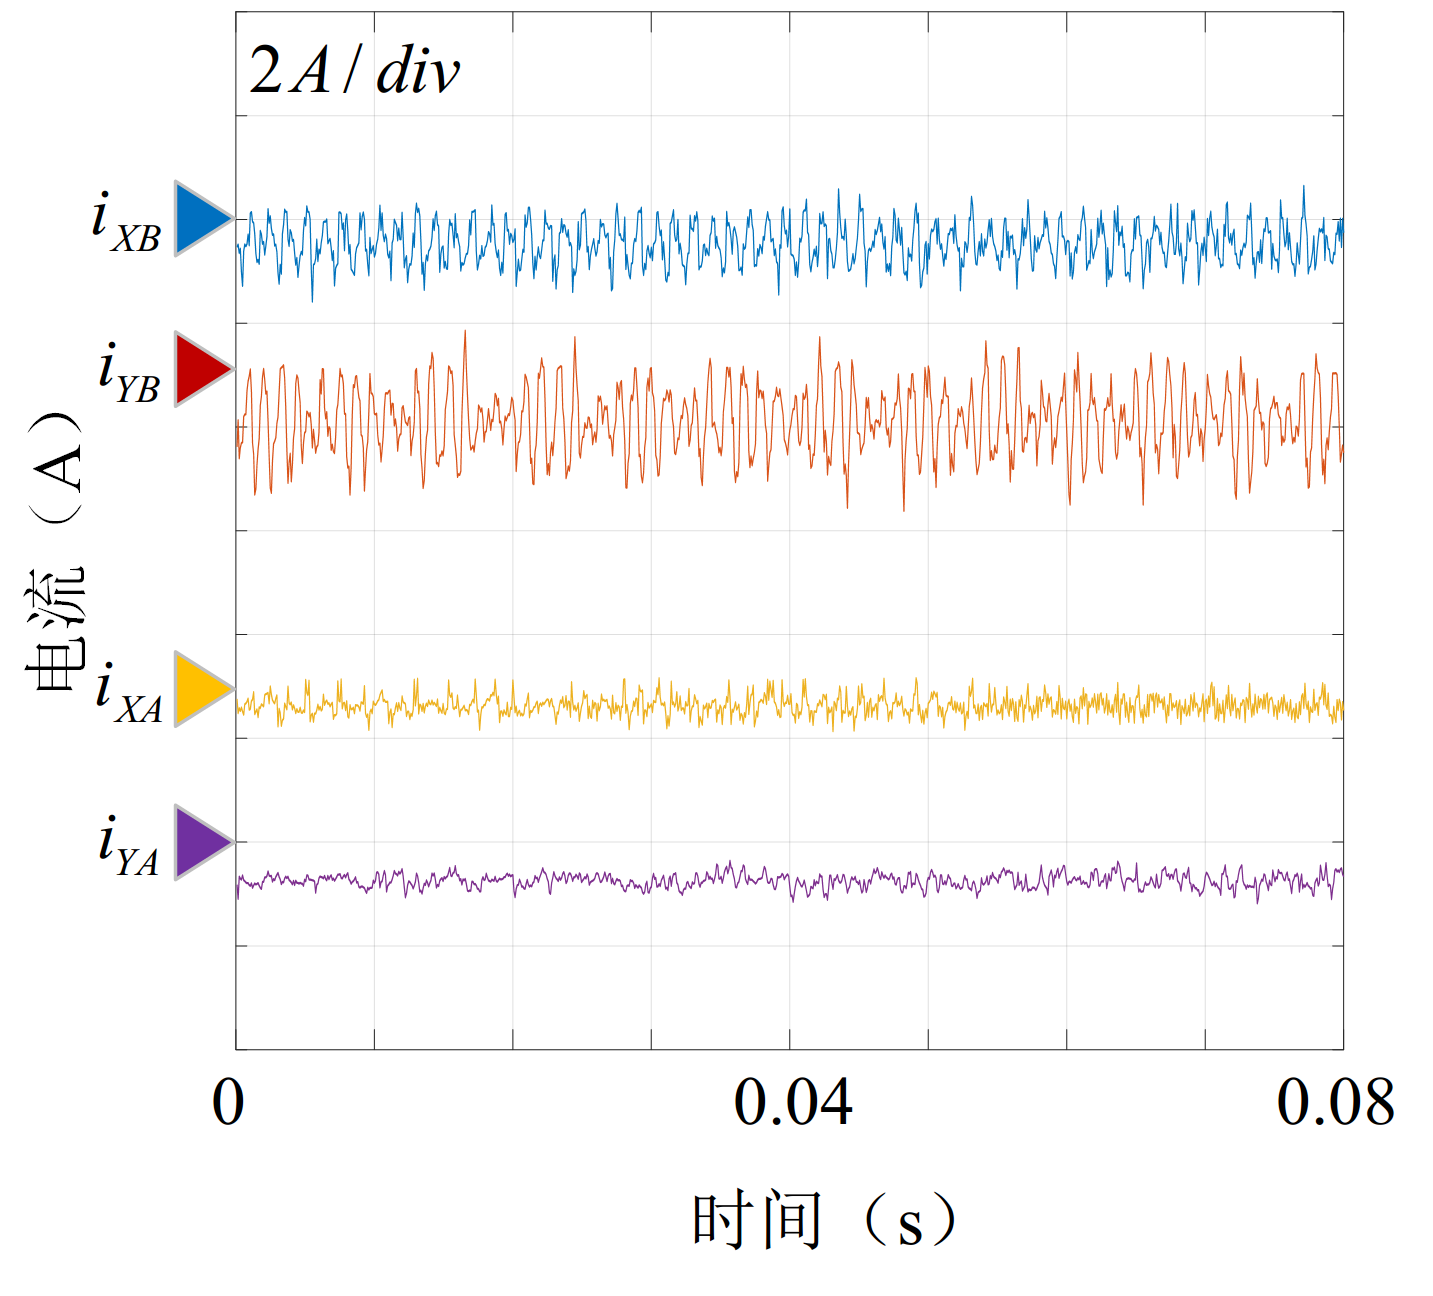
\includegraphics[scale=1.0]{5-s3-i-w1-pid-nf.png}}  
	\caption{加入重复控制器前后控制电流时域波形}  \label{fig:5-s3-i-w1-pid_orc}
\end{figure}

\begin{figure}[h!]
	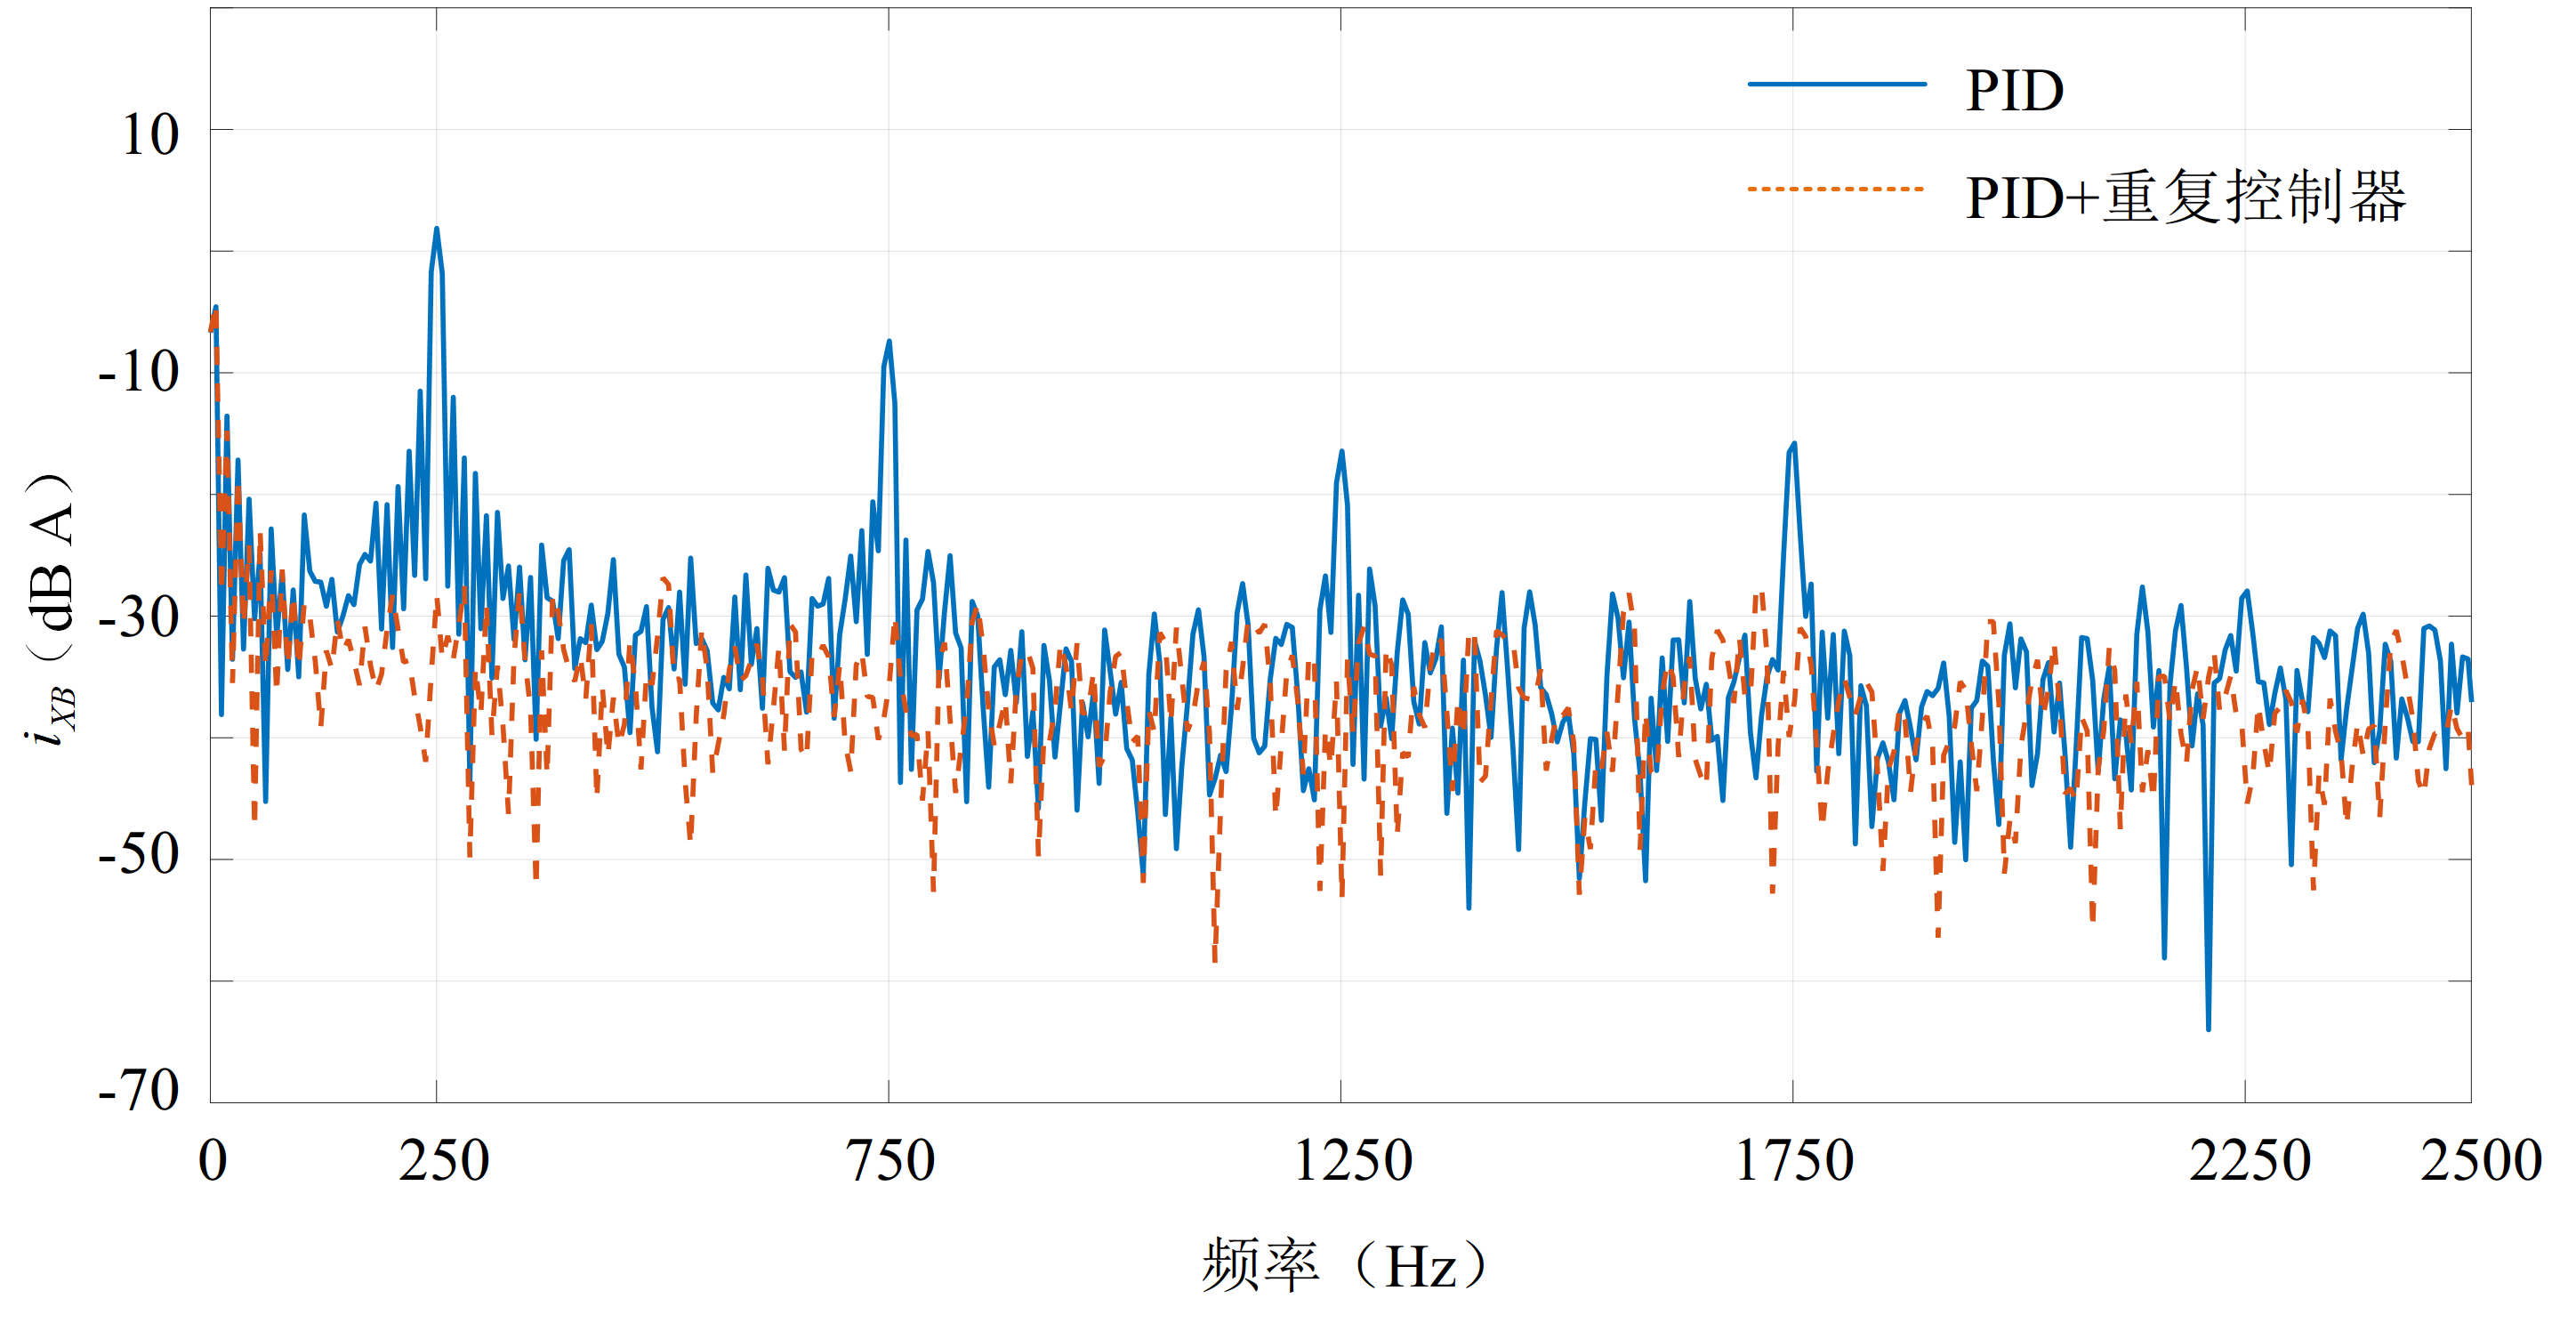
\includegraphics[scale=1.0]{5-s3-i_f-w1-pid_orc.png}
	\caption{加入重复控制器前后$i_{XB}$频谱}
	\label{fig:5-s3-i_f-w1-pid_orc}
\end{figure}

对比分析新型零电流控制方案的效果。\autoref{fig:5-s3-i-w1-pid_orc}~显示了加入重复控制器前后控制电流时域波形。加入重复控制器后,最大的控制电流幅值从\autoref{fig:5-s3-i-w1-pid}~所示的约2A下降到\autoref{fig:5-s3-i-w1-pid-orc}~所示的约1A。\autoref{fig:5-s3-i_f-w1-pid_orc}~显示了加入重复控制器前后$i_{XB}$频谱,从此图中可以清楚看出加入重复控制器前控制电流中包含一、三、五和七次谐波成分,而加入重复控制器后,一、三、五和七次谐波频率处的尖峰消失,谐波电流被有效消除。实验现象说明新型零电流控制方案比传统零电流控制方案可以取得更好的谐波电流抑制效果。

本文使用实时数字控制器和PC端数据采集软件同时采集多路位移信号。软件采样频率为12.5kHz,采样长度为1000。转子在250Hz运转时,加入零电流控制算法后,采集径向通道位移信号和转角信号。通过前文所述的不平衡质量辨识方案,传统零电流控制方案和新型零电流控制方案下辨识出的不平衡质量大小和相位如\autoref{tab:nf_orc_w1}~所示。

\begin{table}[h!]
  \caption[现场动平衡初始配重及辨识质量]{现场动平衡初始配重及辨识质量\label{tab:nf_orc_w1}}
\begin{tabular}{ccc}
    \toprule
    	项目  & 轴端 & 大小和相位 \\
    \midrule
		\multirow{2}{*}{初始配重质量}   
		& A  & $596mg \angle -140^{\circ}$      \\
		& B  & $559mg \angle -125^{\circ}$      \\    
		\multirow{2}{*}{基于陷波器零电流方案辨识的不平衡质量}   
		& A  & $660mg \angle -145^{\circ}$      \\
		& B  & $657mg \angle -125^{\circ}$      \\
		\multirow{2}{*}{基于ZORC零电流方案辨识的不平衡质量} 
		& A  & $648mg \angle -148^{\circ}$      \\
        & B  & $646mg \angle -128^{\circ}$     	\\
		\multirow{2}{*}{实际校正质量(增重)} 
		& A  & $659mg \angle 35^{\circ}$      \\
        & B  & $654mg \angle 55^{\circ}$     	\\        
    \bottomrule
\end{tabular}
\end{table}

从\autoref{tab:nf_orc_w1}~可以看出,基于陷波器零电流方案和基于ZORC零电流方案辨识得到的不平衡质量大小与初始配重质量相比均偏大,解析得到的相位等于或略小于初始配重质量。分析误差原因如下:

(1)由于除初始配重质量外,转子自身存在一定的不平衡质量分布,而该不平衡质量量级较小、分布无法准确测得,且可能导致实际的不平衡质量分布与初始配重质量发生一定偏差;

(2)配重盘上的用于固定配重螺丝的螺纹孔分布间隔为$10^{\circ}$,相位读数仅可精确到$10^{\circ}$。

综合以上原因考虑两种方案的辨识结果,可认为陷波器法辨识的不平衡质量和重复控制器法辨识的不平衡质量精度基本一致。

根据辨识结果理论计算得到的校正质量的大小与辨识的不平衡质量的大小相等,相位相差$180^{\circ}$。实际进行现场动平衡操作时,转子增重通过螺丝孔上加装垫片实现,这种方式增重质量可精确到$10g$,间隔分布的螺丝孔使得增重的相位可精确到$10^{\circ}$。因此实际增重质量与计算校正质量不是严格相等。本实验中的实际增重质量取计算校正质量的附近值,如\autoref{tab:nf_orc_w1}~所示。

\begin{figure}[h!]
	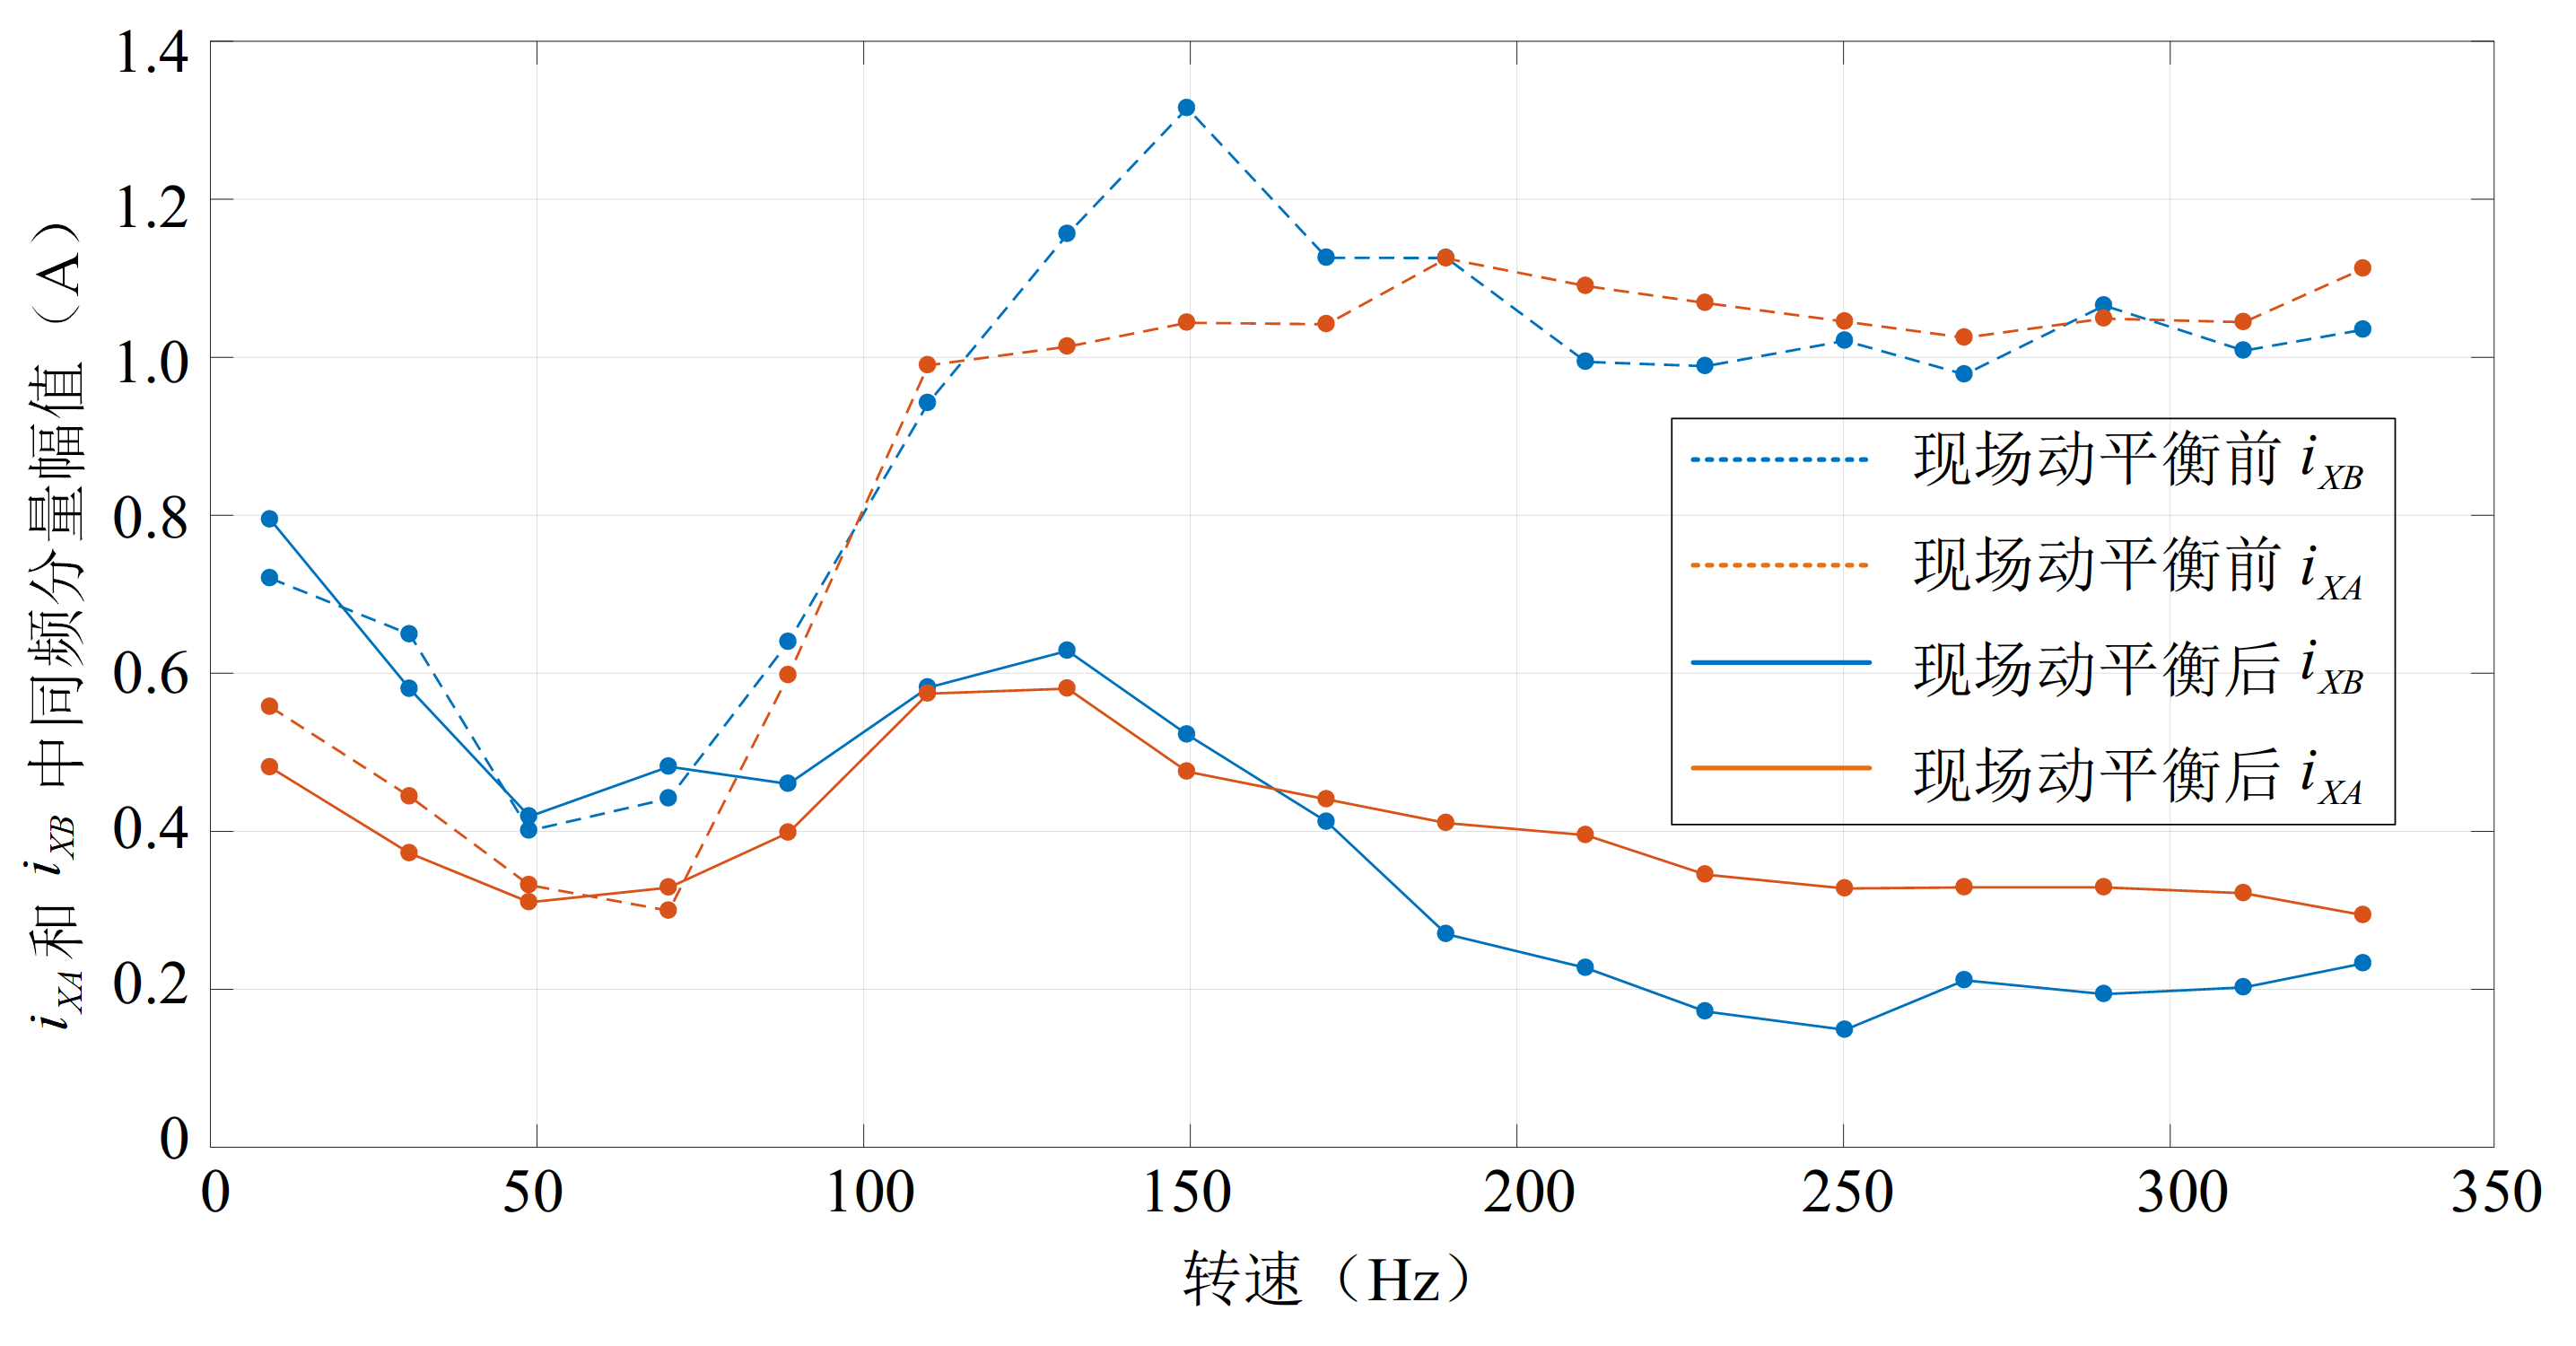
\includegraphics[scale=1.0]{5-s3-i-w1w2.png}
	\caption{现场动平衡前后$i_{XB}$、$i_{XA}$同频分量幅值}
	\label{fig:5-s3-i-w1w2}
\end{figure}

\autoref{fig:5-s3-i-w1w2}~显示了现场动平衡前后控制电流中同频分量幅值。从图中可以看到,现场动平衡之前A端磁轴承和B端磁轴承中的控制电流$i_{XA}$和$i_{XB}$中的同频分量的幅值随着转速变化而变化,从10Hz处的0.7A附近先下降到约0.4A,然后上升到约1.1A,之后稳定在1.1A附近。完成现场动平衡之后,在90Hz前$i_{xA}$和$i_{xB}$中的同频分量的幅值与现场动平衡之前没有显著的变化,在90Hz之后,随着转速继续升高,二者则始终比现场动平衡之前的值小得多,稳定在约0.3A附近。该动平衡方法使控制电流同频振动幅值在大转速范围内实现显著下降。

\begin{figure}[h!]
	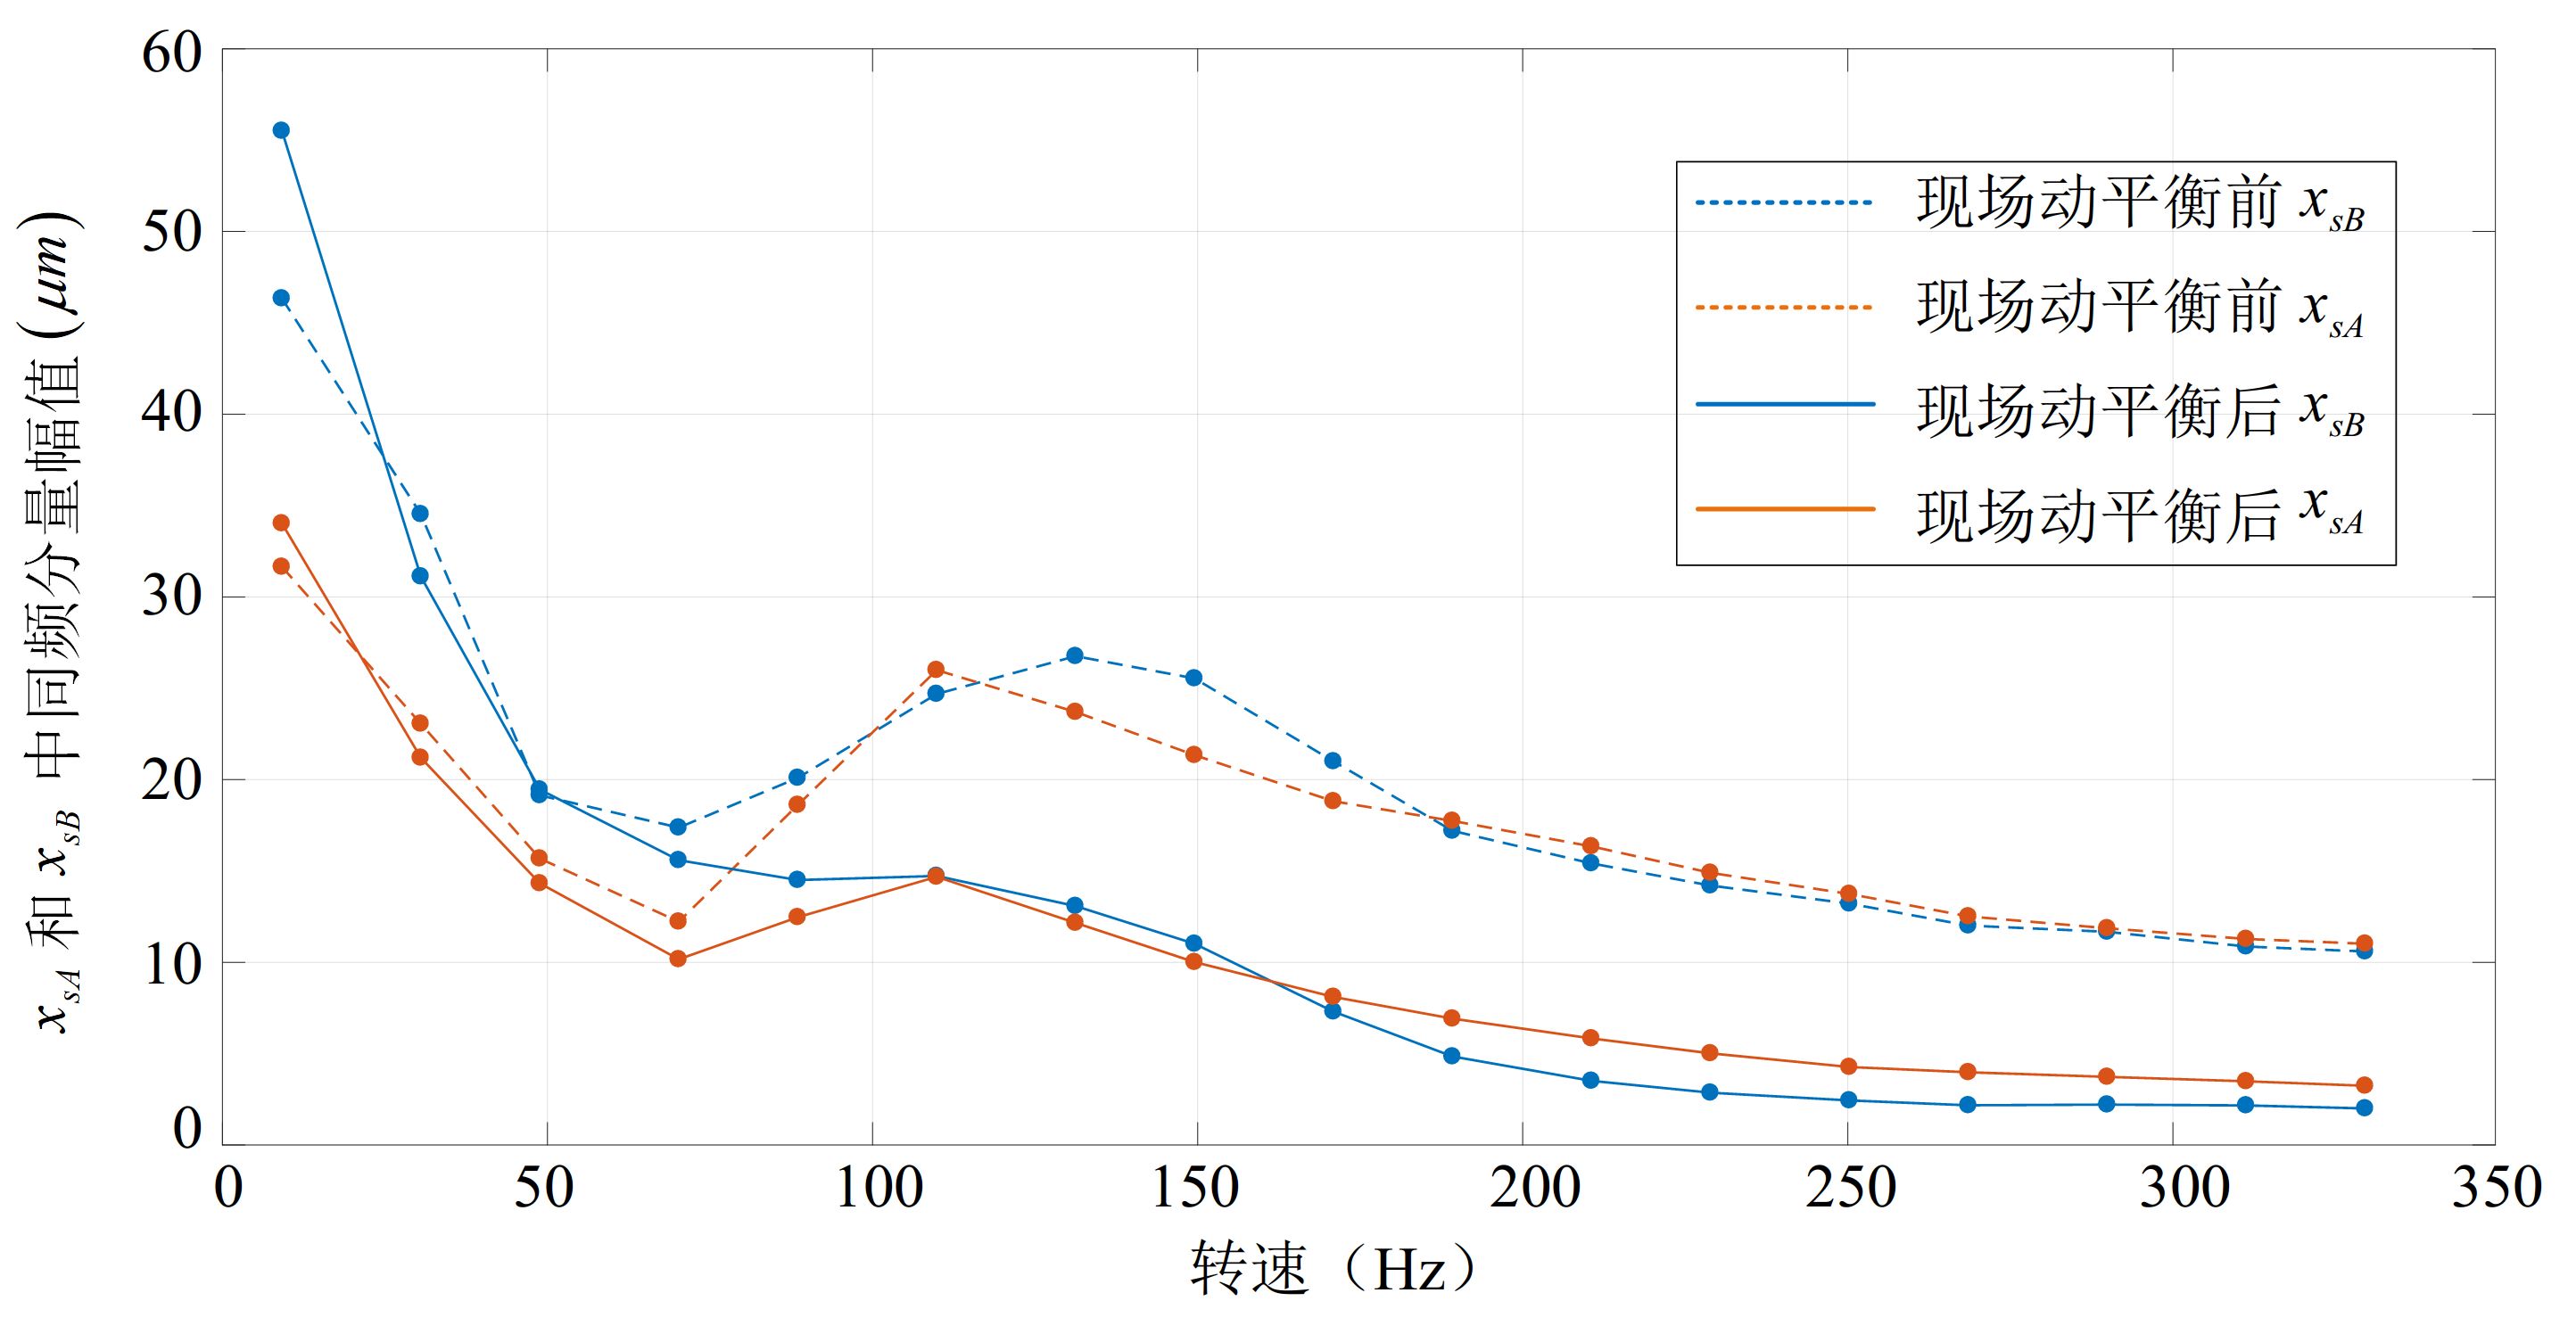
\includegraphics[scale=1.0]{5-s3-x-w1w2.png}
	\caption{现场动平衡前后$x_{sB}$、$x_{sA}$同频分量幅值}
	\label{fig:5-s3-x-w1w2}
\end{figure}

\autoref{fig:5-s3-x-w1w2}~显示了现场动平衡前后转子轴端位移中同频分量幅值。从图中可以看到,现场动平衡之前A端磁轴承和B端磁轴承中的位移$x_{sA}$和$x_{sB}$中的同频分量的幅值随着转速变化而变化,二者先从10Hz处约$32 \mu m$和$48 \mu m$处先下降再上升到约$28\mu m$,最后下降稳定到约$12 \mu m$;现场动平衡之后,90Hz前$x_{sA}$和$x_{sB}$与现场动平衡之前无显著区别。90Hz后,$x_{sA}$和$x_{sB}$中的同频分量幅值始终小于现场动平衡之前的幅值,最终稳定在约$4 \mu m$处。\autoref{fig:5-s3-i-w1w2}~和\autoref{fig:5-s3-x-w1w2}~所示的实验现象说明本文采取的基于重复控制器的现场动平衡方法有明显振动抑制效果。

\begin{figure}[h!]
	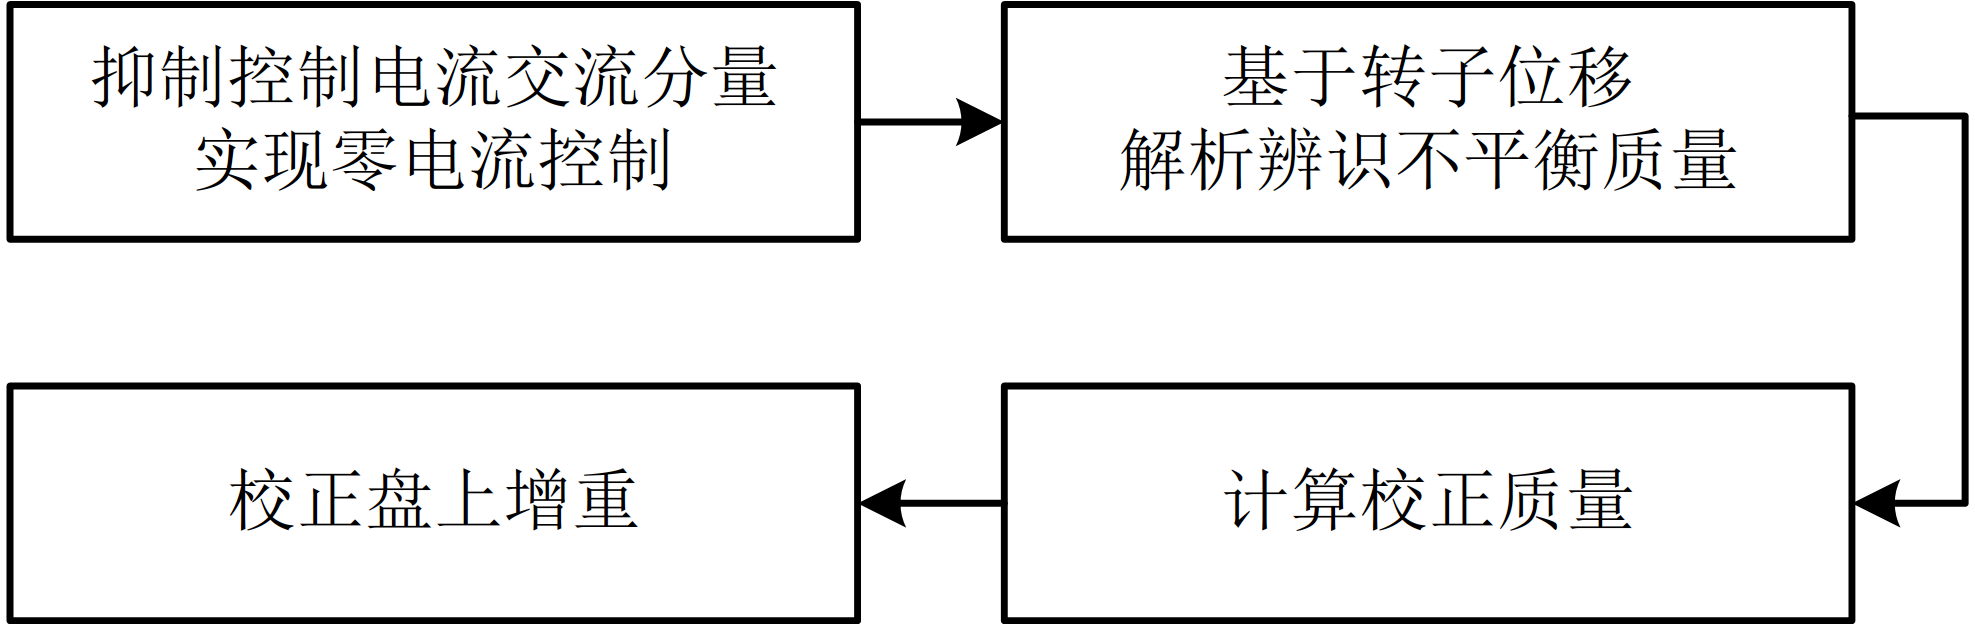
\includegraphics[scale=1.0]{4-field_flow.png}
	\caption{基于重复控制器法的现场动平衡方案流程图}
	\label{fig:4-field_flow}
\end{figure}	

\section{本章小结}
本章提出基于ZORC的现场动平衡方法,论证了该方法实现零电流控制、辨识和校正不平衡质量的可行性,其步骤可以总结为\autoref{fig:4-field_flow}~所示。基于该方案进行现场动平衡后,同频振动电流以及同频振动位移均取得显著的降低,验证了ZORC的现场动平衡理论方法的可行性。与传统现场动平衡方法相比,该方法无需试重,且可达到与基于陷波器的现场动平衡方法同等的现场动平衡精度。

\chapter{磁悬浮轴承数字控制平台的实验研究}
磁悬浮轴承系统包含机械部分和控制部分,包括磁悬浮轴承及其支撑的转子以及控制板卡和控制软件程序,本章介绍控制板卡的硬件设计和软件设计。

\section{硬件设计}

硬件、软件组成的完整磁悬浮轴承数字控制平台如\autoref{fig:5-testrig}~所示。其中磁悬浮离心机中的转子旋转由逆变器驱动,转子悬浮由磁悬浮轴承系统控制。
\begin{figure}[h!]
	\includegraphics[scale=1.0]{5-testrig.png}
	\caption{磁悬浮轴承数字控制平台}
	\label{fig:5-testrig}
\end{figure}

磁悬浮轴承系统硬件部分包括位移传感器、控制板卡、功率放大器和上位机程序,加速度传感器和示波器用于监测系统运行状态。磁悬浮轴承系统内的结构与数据交互关系如\autoref{fig:5-component}~所示。

\begin{figure}[h!]
	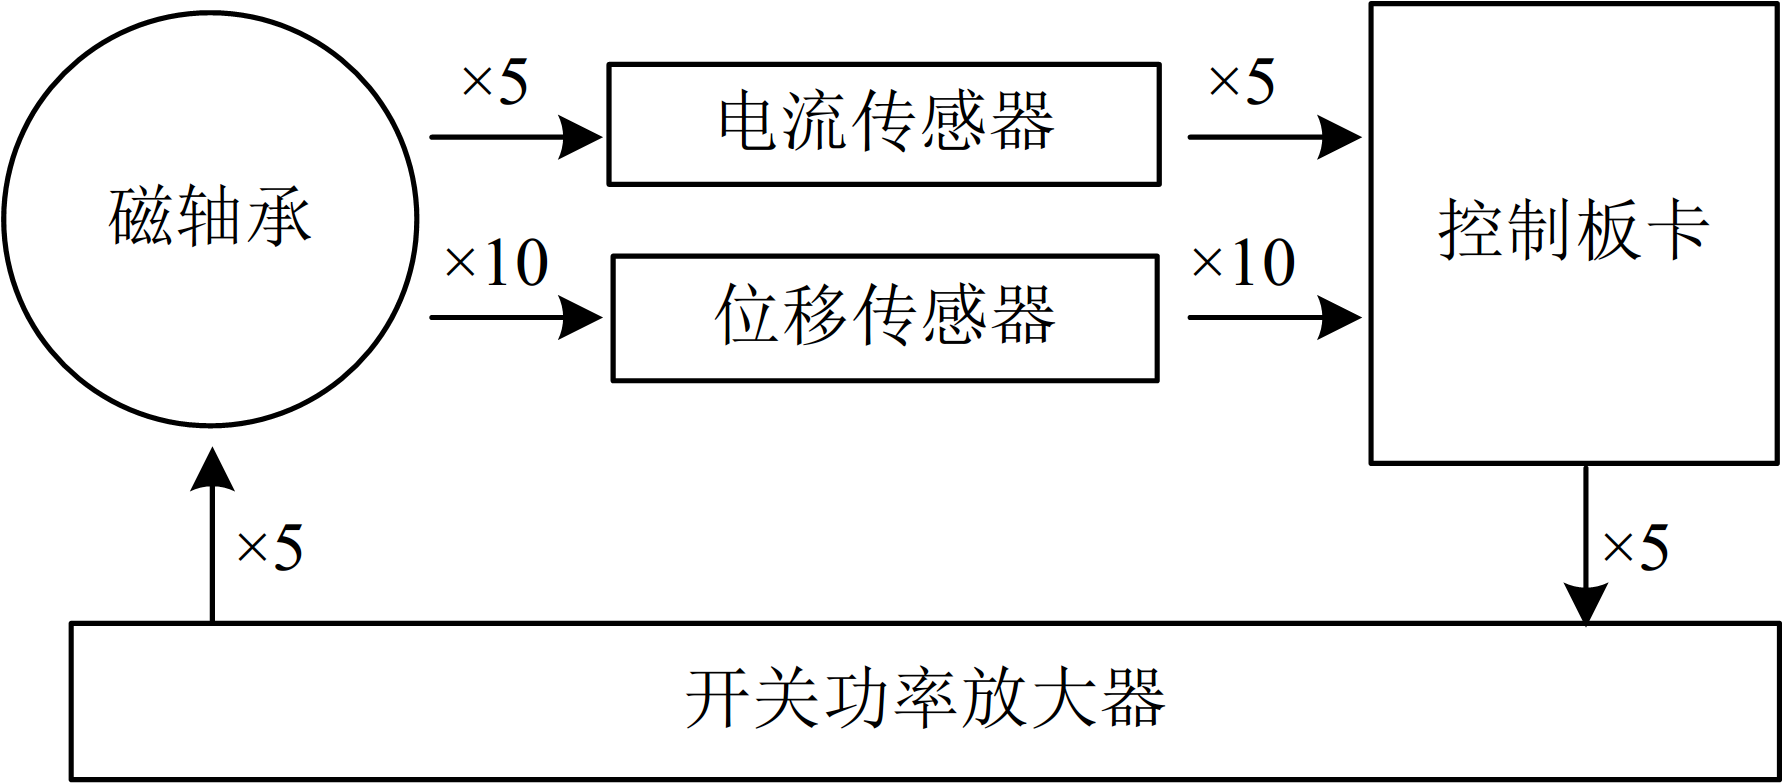
\includegraphics[scale=1.0]{5-component.png}
	\caption{磁悬浮轴承系统硬件组成}
	\label{fig:5-component}
\end{figure}

位移传感器用于实时采集转子位置,作为反馈量输入到控制器中。位移传感器的信号质量直接决定了闭环系统控制性能。本文采用电涡流位移传感器,其测量线性范围是$0.10 \sim 1.10mm$,标准灵敏度为$20.00V/mm$,非线性度为$0.8\%$。位移传感器将转子位移量转换成电压输出,经模数转换芯片(Analog to Digital Converter,简称ADC)采样后即得到数字量输出。本文使用的ADC芯片输入模拟电压信号幅值范围$-10V \sim 10V$,对应数字量输出范围为$-32768 \sim 32767$。则实际位移值到ADC采样数字量之间的系数关系为:
\begin{equation}
\frac{ADC_{reading}}{Displacement} = \frac{20.00V}{1 \times 10^{-3}m} \times \frac{32767}{10V} = 6.5534 \times 10^6/m
\end{equation}

电流传感器用于实时采样磁轴承控制电流值,作为反馈量输入到控制器中。本文研究的磁悬浮离心压缩机用的磁悬浮轴承的额定电流是$-6A\sim 6A$,采用电阻采样式电流传感器。采样电阻阻值为$31m\Omega$,经一级隔离运算放大器放大8.2倍,再经过一级运算放大器放大10倍后,输入到ADC进行采样。实际电流值到ADC采样数字量之间的系数关系为:
\begin{equation}
\frac{ADC_{reading}}{Current} = 31 \times 10^{-3}V \times 8.2 \times 10 \times \frac{32767}{10V} \times \frac{1}{1A} = 8329.4/A
\end{equation}

开关功率放大器是磁悬浮轴承执行部件之一,其将控制算法输出的参考电流转换成线圈中的实际电流,使得线圈可以产生磁悬浮力。本文采用全桥式开关功率放大器,母线电压选取为$50V$。五自由度线圈控制共需五组拓扑一致的全桥电路,其中一路全桥电路如\autoref{fig:5-amplifier}~所示。基于滞环控制方案使开关管Q1、Q4和Q2、Q3轮流导通,来控制磁轴承控制电流值跟踪电流给定值。

\begin{figure}[h!]
	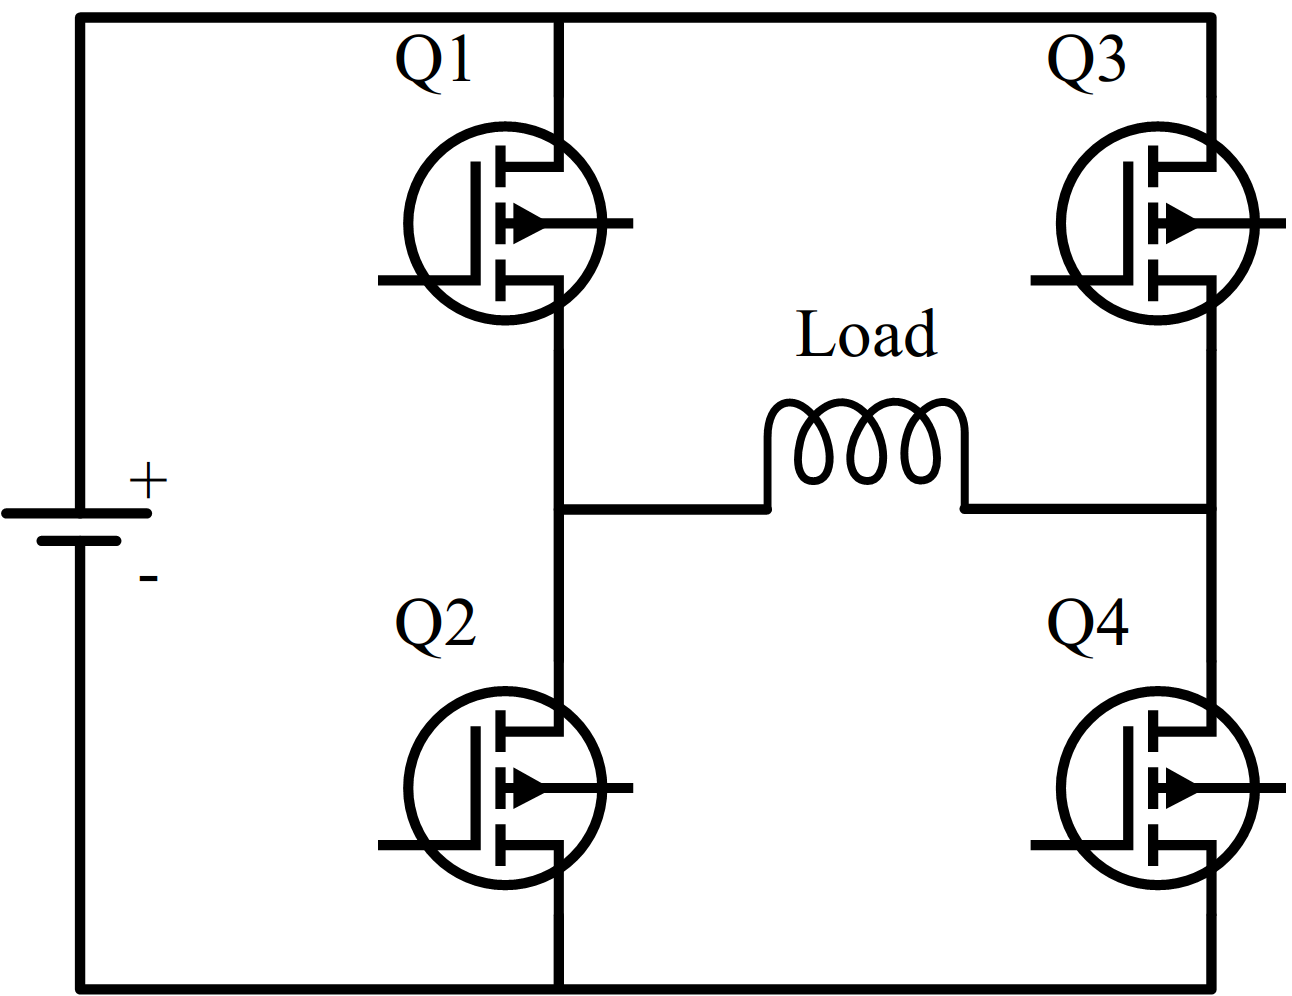
\includegraphics[scale=1.0]{5-amplifier.png}
	\caption{开关功率放大器单路全桥拓扑}
	\label{fig:5-amplifier}
\end{figure}

控制板卡包含一块STM32F407芯片和一块Cyclone IV EP4CE40芯片,以及信号调理电路、驱动隔离电路等外围电路。STM32F4系列单片机是意法半导体公司(ST)推出的基于ARM Cortex-M4内核的高性能微控制器,搭载NVM技术和ART加速器技术,使得该系列单片机的计算性能可达225DMIPS(主频运行于180MHz)。此外,其集成的单周期DSP指令和浮点运算单元(Floating Point Unit,简称FPU),具备高效完成复杂数学浮点运算的能力。本文使用的STM32F407ZET6参数如\autoref{tab:stm32_para}~所示。

\begin{table}[h!]
  \caption[STM32F407ZET6性能参数]{STM32F407ZET6性能参数\label{tab:stm32_para}}
  \begin{tabular}{cc}
    \toprule
    模块 & 性能值 \\
    \midrule
    Flash & 512KB\\
    RAM & 192KB\\
    定时器 & 12$\times$ 16-bit + 2$\times$ 32-bit\\
    ADC & 24 $\times$ 12-bit\\
    DAC & 2 $\times$ 12-bit\\
    USART + UART & 4 + 2\\
    Ethernet & 1	\\
    \bottomrule
  \end{tabular}
\end{table}

Cyclone IV E系列芯片是Intel公司2009年推出的低成本、低功耗、较高性能的FPGA(Field Programmable Gate Array,简称FPGA)芯片解决方案。Cyclone IV E系列基于优化的60纳米低功耗制程技术构建,配备逻辑单元、片上存储单元、片上乘法器、锁相环(Phase Locked Loop,简称PLL)、全局时钟网络以及数量众多的普通I/O端口。本文选用的是Cyclone IV EP4CE40F23I7,其主要参数如\autoref{tab:fpga_para}~所示。

\begin{table}[h!]
  \caption[Cyclone IV EP4CE40F23I7性能参数]{Cyclone IV EP4CE40F23I7性能参数\label{tab:fpga_para}}
  \begin{tabular}{cc}
    \toprule
    模块 & 性能值 \\
    \midrule
    逻辑单元 & 39600\\
    嵌入式存储 & 1134KB\\
    嵌入式18$\times$18乘法器 & 116\\
    通用型PLL & 4\\
    全局时钟网络 & 20\\
    用户I/O组 & 8\\
    最大用户I/O & 532	\\
    \bottomrule
  \end{tabular}
\end{table}

\section{软件设计}
磁悬浮轴承控制系统软件部分的实现基于前文所述的硬件组件和板载电路,软件控制目标是使转子在高速旋转时,仍稳定悬浮在磁悬浮轴承中心,且具备抗干扰和抗冲击能力。为实现该目标,本文搭建了一套由上位机程序、STM32单片机程序和FPGA程序共同组成的磁悬浮轴承控制软件。顶层软件结构如\autoref{fig:5-software_top}~所示。FPGA拥有高速并行计算能力,因此磁轴承闭环控制中的外环和内环控制均部署于其中计算。为防止系统意外故障致转子跌落损伤轴承,FPGA实时监控转子位移波形,在检测到异常发生时自动切断电机驱动器。借助于STM32F4系列的丰富通讯接口,其承担“数据中转站”的功能——采集FPGA中的控制状态量然后传输给PC,或接收PC指令然后写入到FPGA控制寄存器中。此外,STM32F4采集和监测电机和轴承温度,保证系统工作温度正常。PC上运行基于Matlab/Appdesigner模块设计的上位机程序,用于读写FPGA控制状态量以及进行数据采集与分析。

\begin{figure}[h!]
	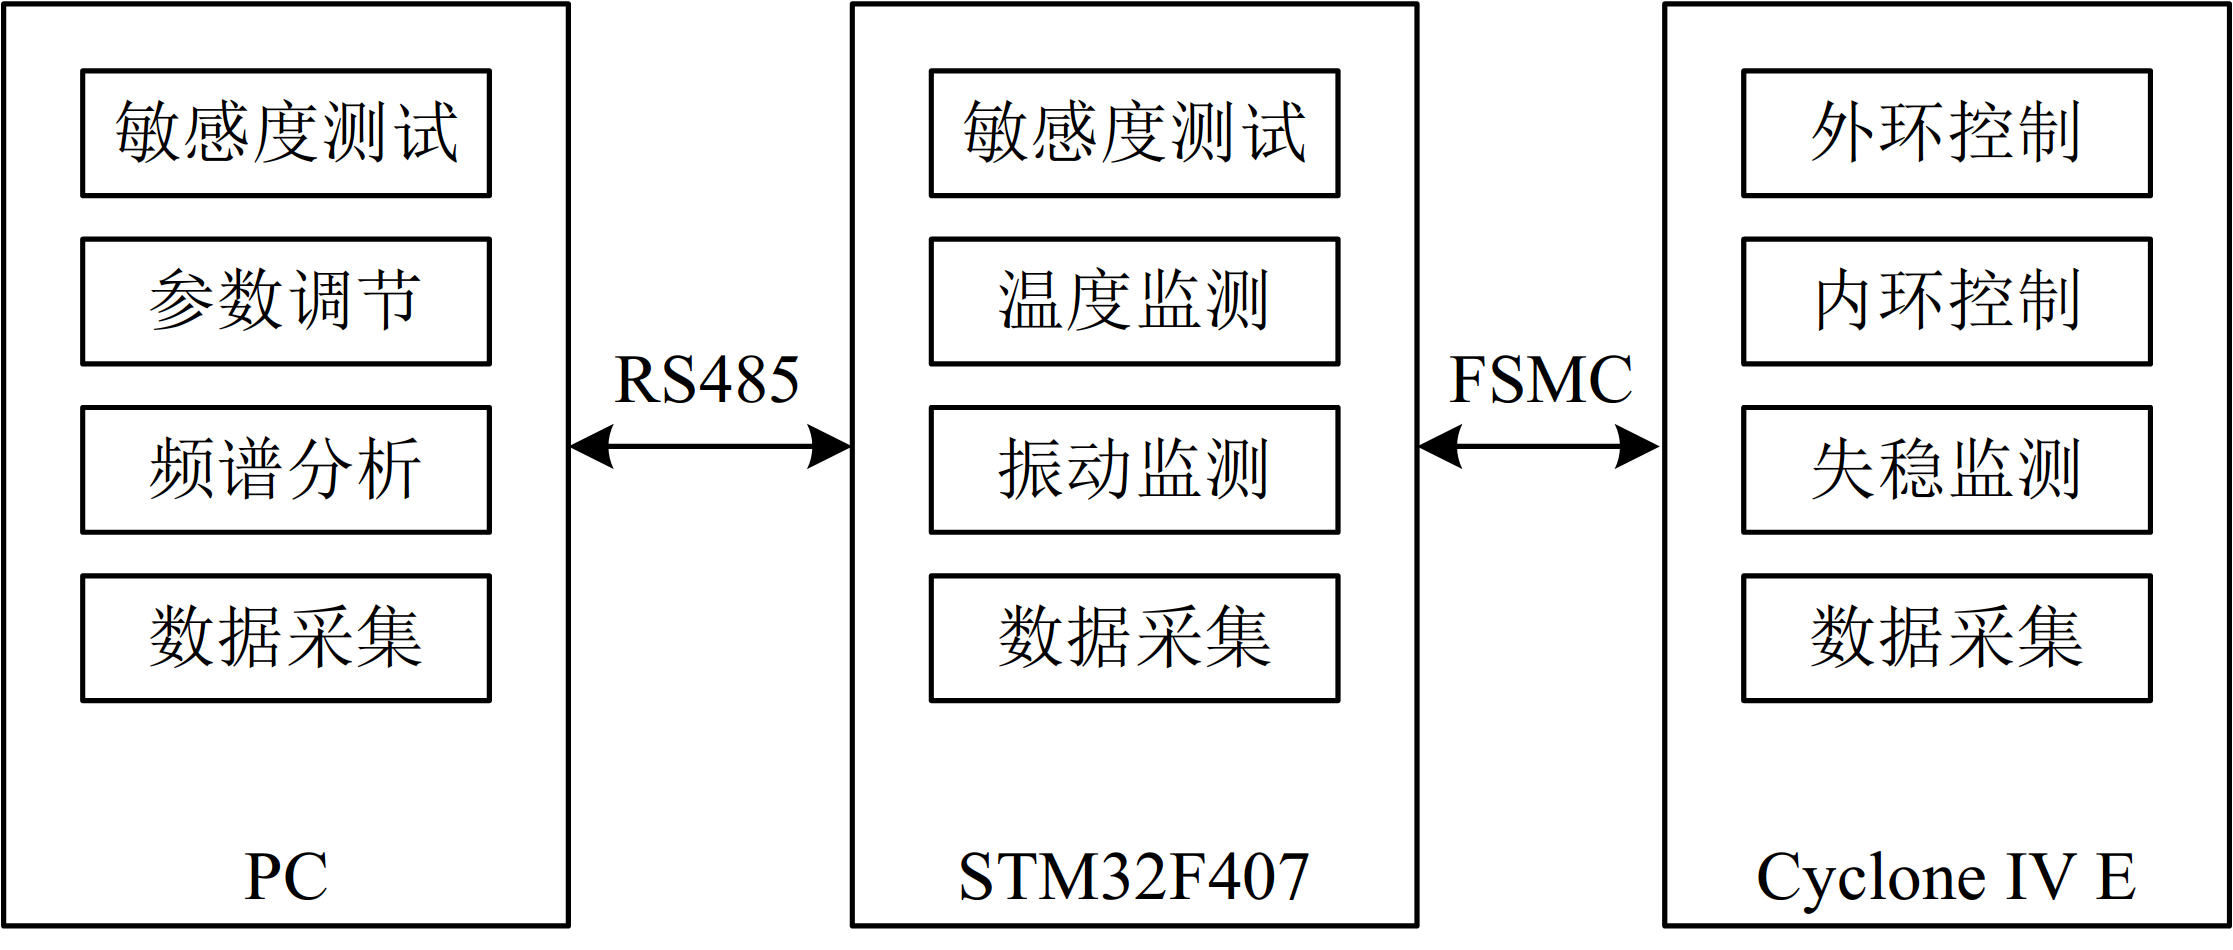
\includegraphics[scale=1.0]{5-software_top.png}
	\caption{磁轴承系统控制顶层软件结构}
	\label{fig:5-software_top}
\end{figure}

\subsection{实时控制程序}
实时控制程序是控制磁悬浮轴承的核心程序,包括内环控制和外环控制,如\autoref{fig:5-software_rtcontrol}~所示。其中外环是指转子位移控制:位移传感器采集转子位置,外环控制器目标是使转子实际位置跟踪人为给定位置。内环是指磁悬浮轴承电流控制:磁悬浮轴承通过线圈中的控制电流激发磁场,进而产生磁悬浮力控制转子位置,内环控制器目标是使线圈实际电流跟踪外环控制器输出给定电流。

\begin{figure}[h!]
	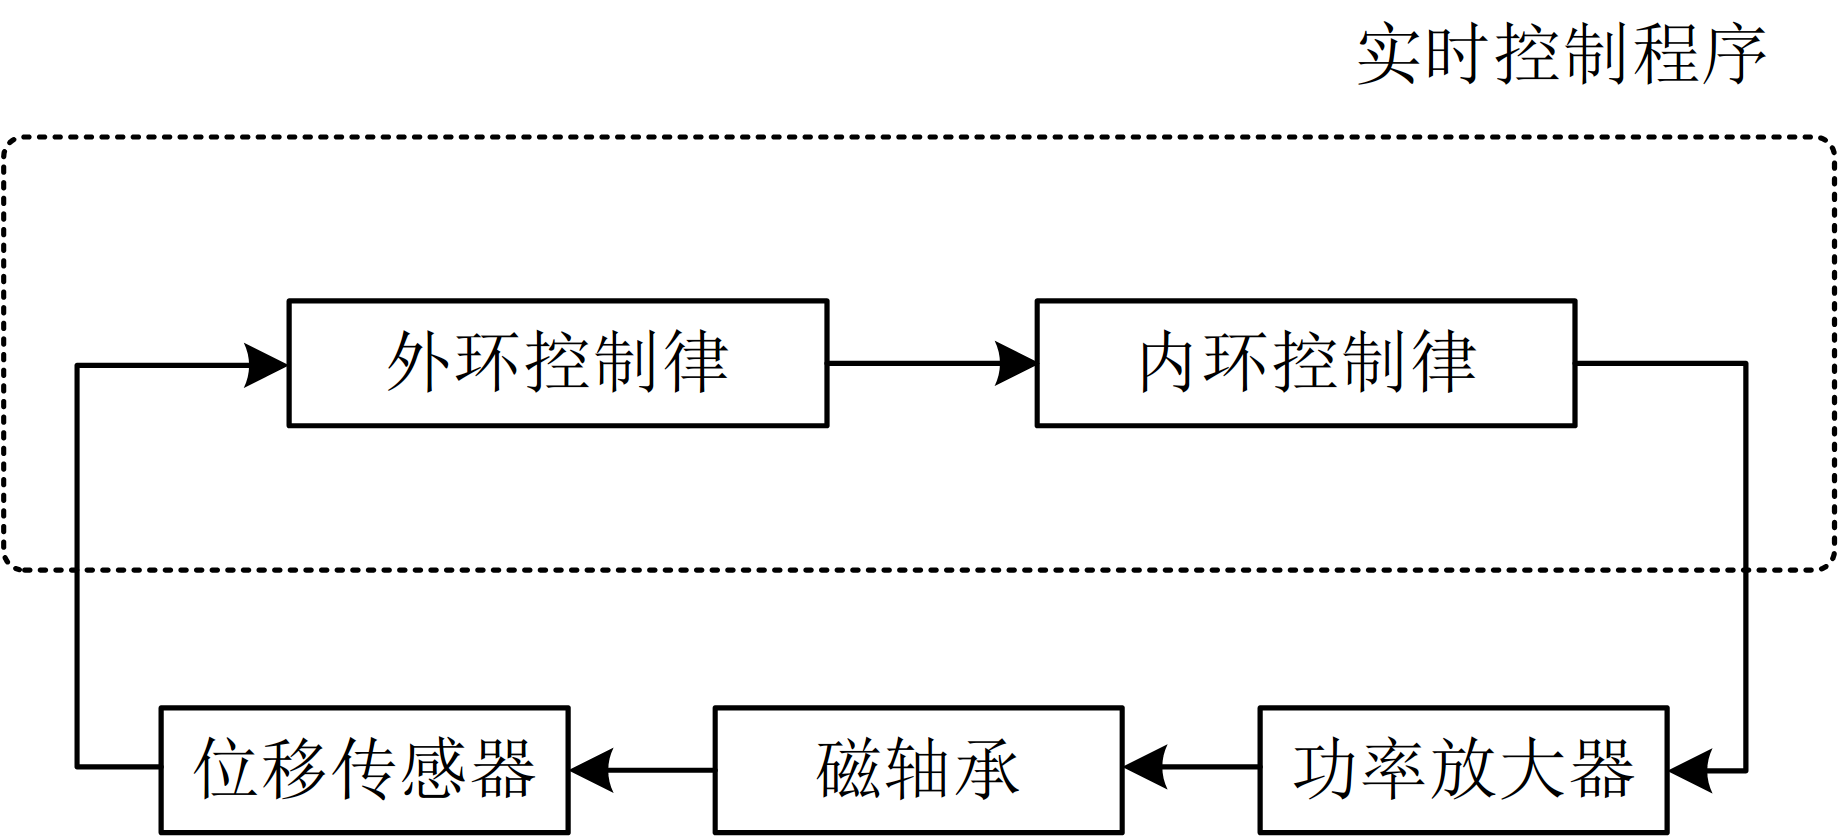
\includegraphics[scale=1.0]{5-software_rtcontrol.png}
	\caption{磁轴承系统实时控制程序}
	\label{fig:5-software_rtcontrol}
\end{figure}

\subsection{用户交互程序}
用户交互程序包括参数调节程序和输出敏感度函数测试程序。

\begin{figure}[h!]
	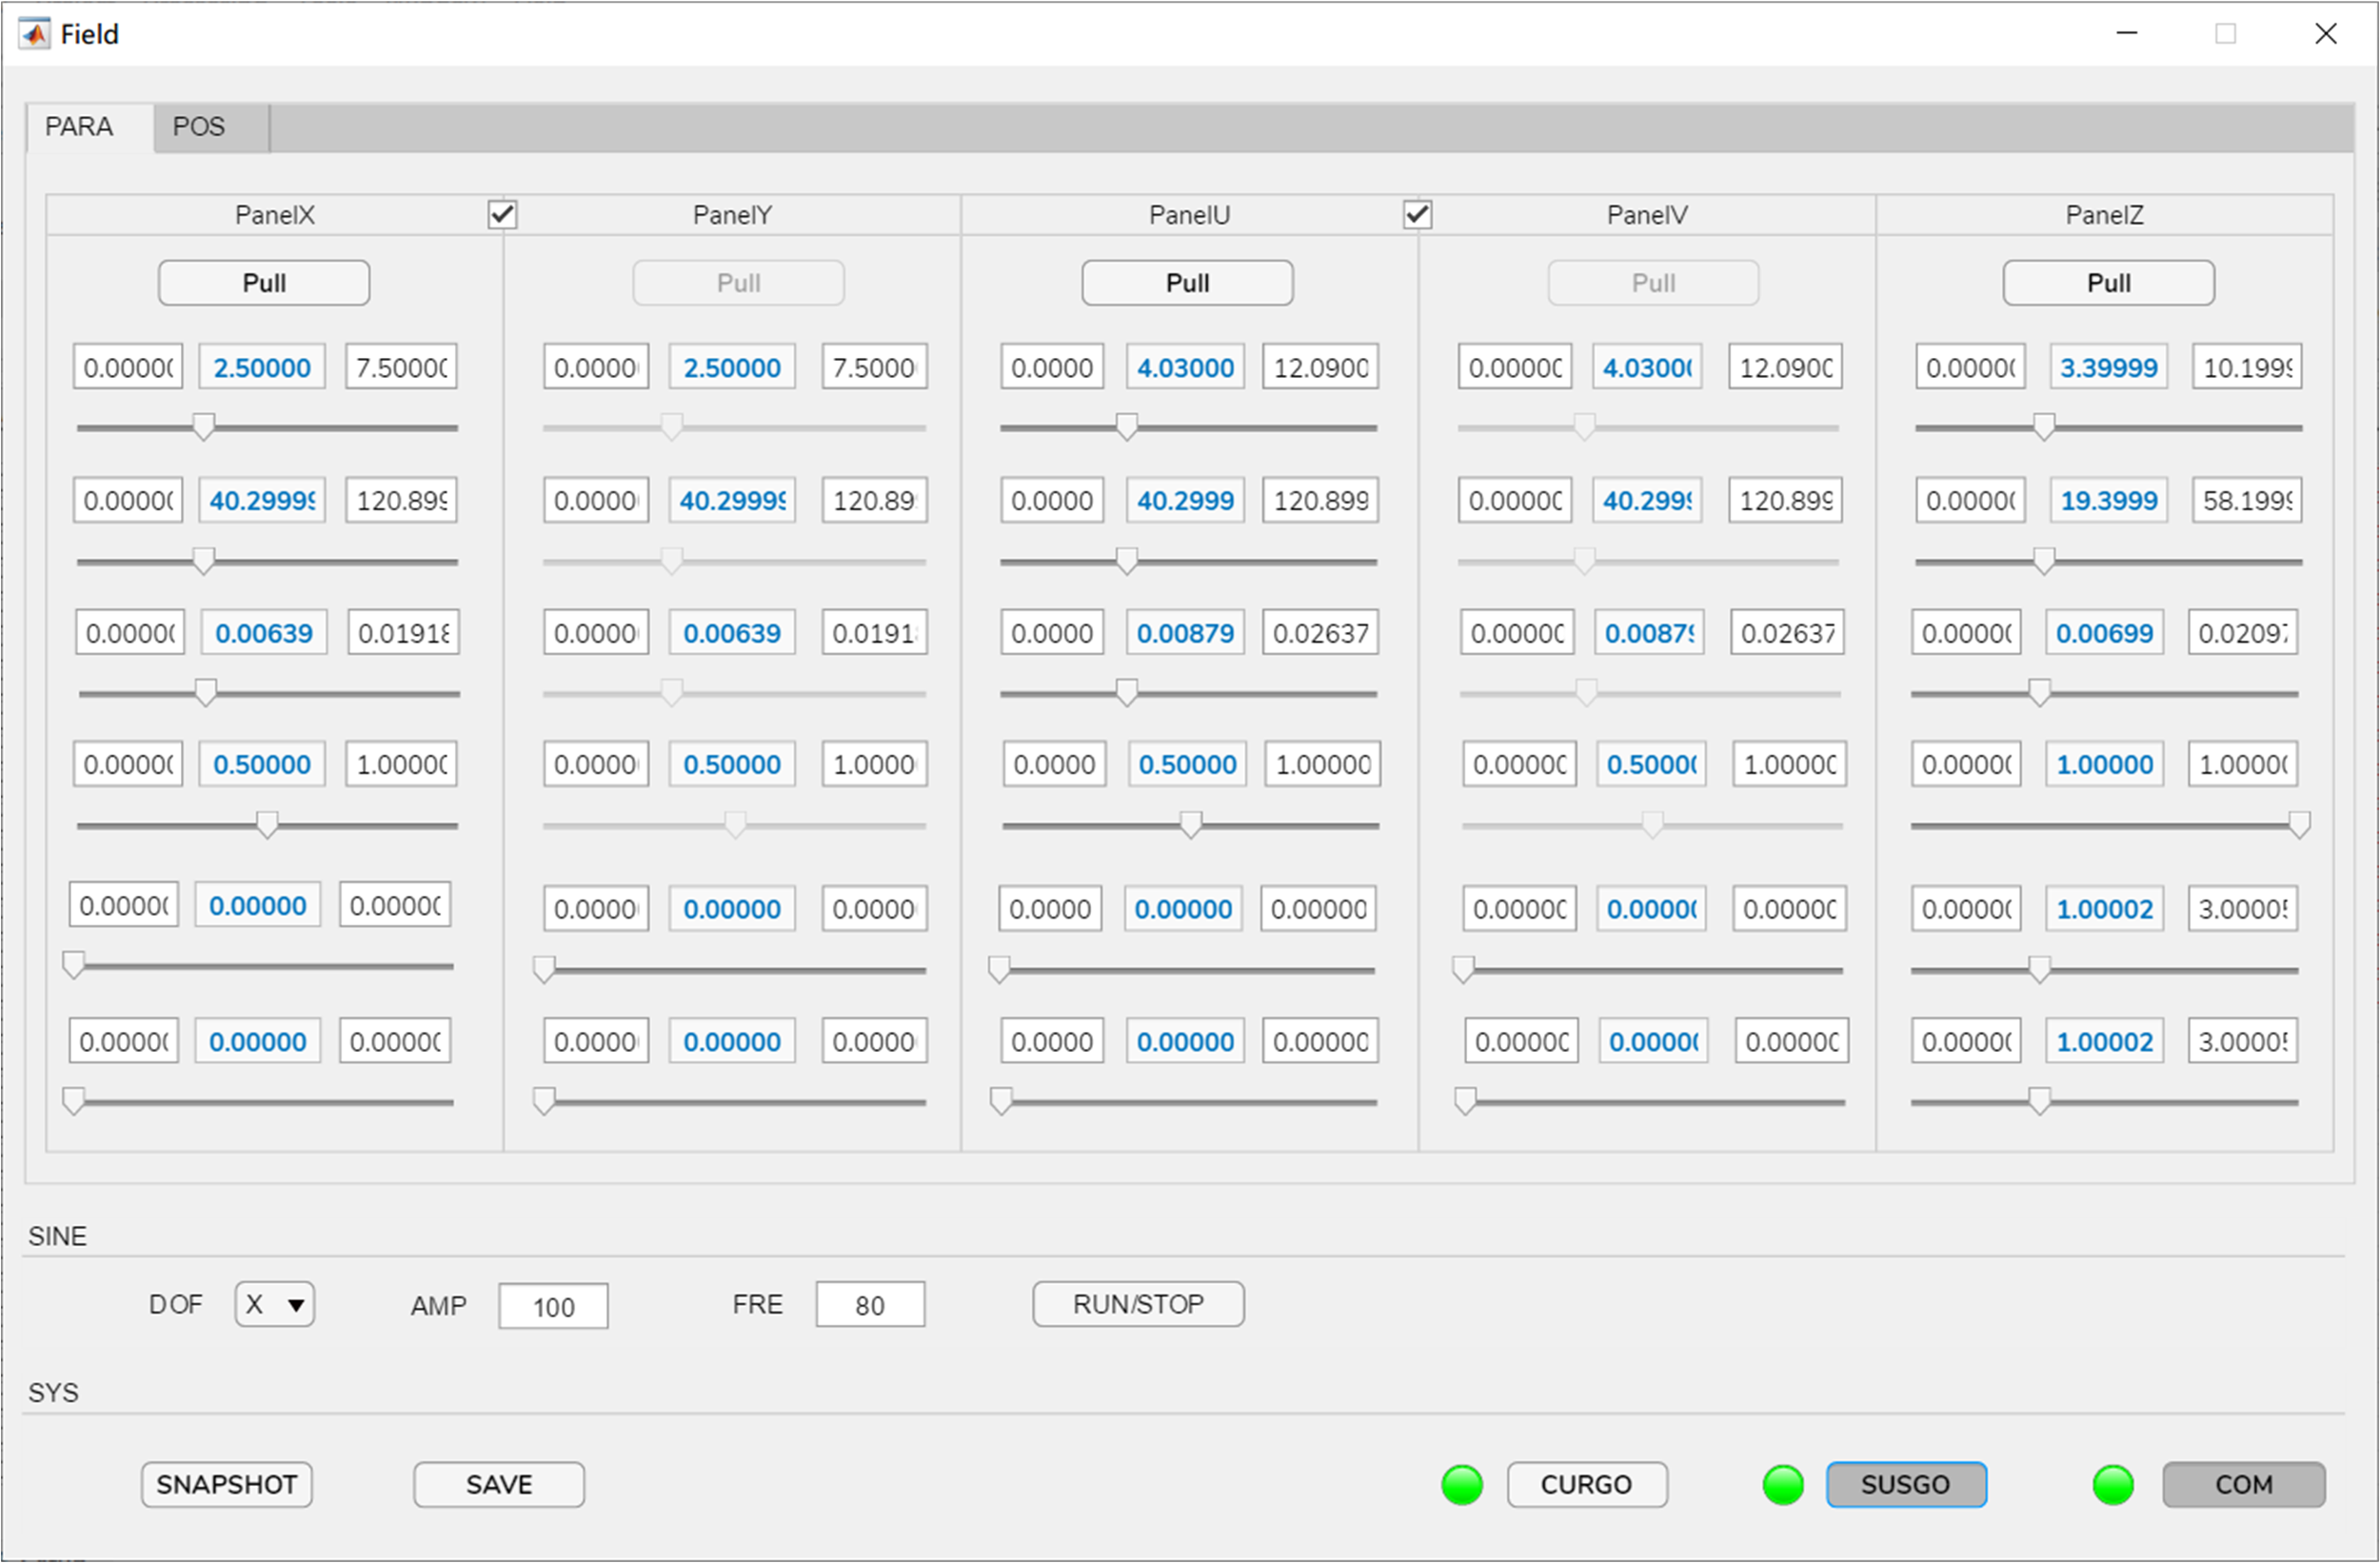
\includegraphics[scale=1.0]{5-software_para.png}
	\caption{磁轴承系统参数调节程序}
	\label{fig:5-software_para}
\end{figure}

\begin{figure}[h!]
	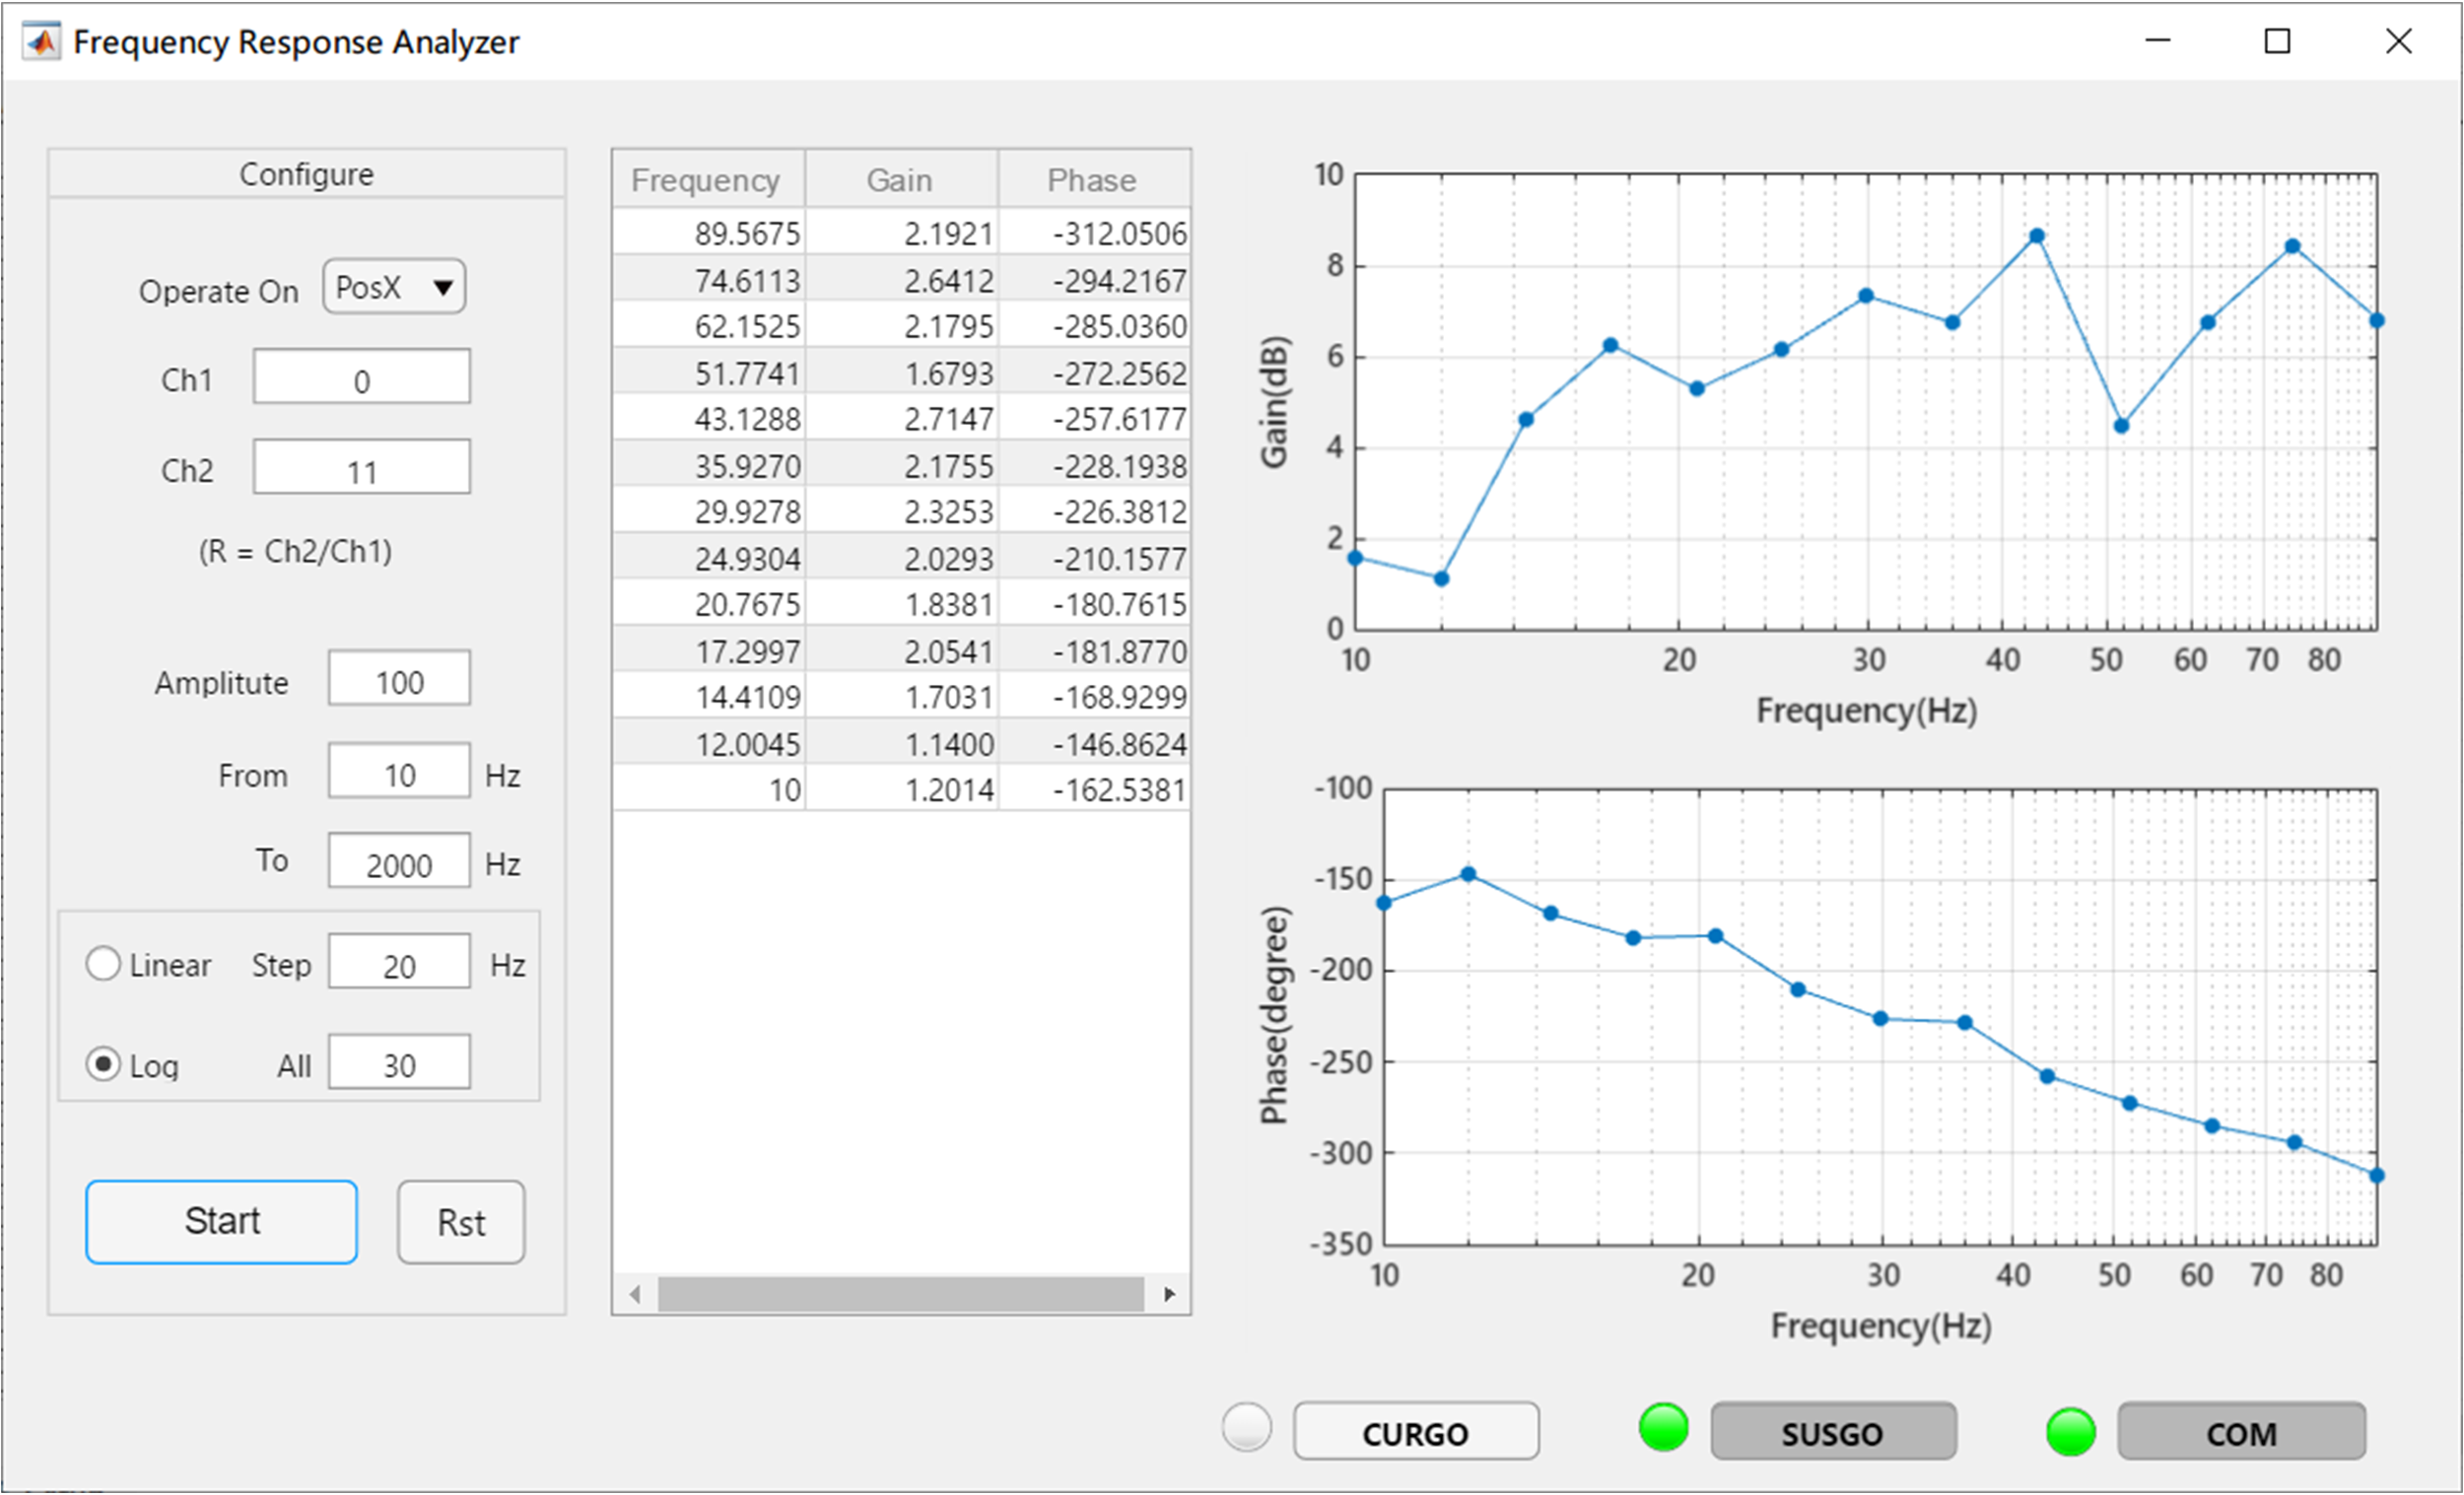
\includegraphics[scale=1.0]{5-software_sen.png}
	\caption{磁轴承系统输出敏感度函数测量程序}
	\label{fig:5-software_sen}
\end{figure}

外环控制器和内环控制器的参数需要根据系统仿真设计值进行初步设计,然而现场根据磁悬浮电机运行状况进行进一步细致调节。磁悬浮轴承双环控制器参数多(约四十个可调参数),且通常需要连续调节以观察转子控制效果。传统参数调节方式有在程序内常量方式写入到Flash中,但该方法不适合需要频繁修改参数的场景;另一种常规方法是通过编程软件中的变量观察窗口进行参数手动输入。以上两种传统参数调节方式无法满足本文设计的双环控制器参数调节需求,因此本文开发桌面版参数调节程序来完成参数调节任务。

本文开发的参数调节程序如\autoref{fig:5-software_para}~所示。使用该程序可以单独调节每一自由度的控制参数,也可以联动调节磁悬浮轴承单端的两个自由度参数。外环和内环的每一个参数的调节范围可任意设置,通过拖动滚动条实现该参数连续变化调节。该软件使用步骤为:控制板卡上电后启动该软件,依次点击各个自由度的【Pull】按钮读取该自由度参数的当前值。手动设置各个参数的范围,拖拉滚动条即可将新的参数值写入到控制板卡上。完成参数调节后退出软件。

输出敏感度函数测量程序用于测试各个自由度的输出敏感度函数,其原理是在给定位移信号上叠加一定幅值和一定频率的正弦信号用作激励,采集反馈位移信号的幅值和相位当做响应,通过测量激励信号和响应信号在一定频率区间上的增益衰减和相位偏差,可以得到该自由度的频率响应特性,即输出敏感度函数。

输出敏感度函数测量程序如\autoref{fig:5-software_sen}~所示。该程序可以设置激励信号的幅值和频率、设置激励信号频率扫描范围,测量过程实时显示已扫描频率点的测量结果。该软件使用步骤为:控制板上电后,运行该程序,点击【SUSGO】按钮启动转子悬浮。依次设置测量自由度、激励信号幅值、扫描频率范围后,点击【Start】按钮。程序开始运行测量程序。测量过程中,列表会显示前序扫描频率点和扫描结果,图框中显示频率-幅值曲线和频率-相位曲线。所有频率扫描完成后,可以选择继续测量下一通道。完成测量后退出软件。


\section{本章小结}
本章介绍了基于STM32F407芯片和Cyclone IV EP4CE40芯片的高性能实时数字控制平台,该数字控制平台包含下位机实时控制程序和上位机参数调节和数据采集程序,可实现以10$\sim$20kHz频率控制十路位移信号采样、五路电流信号采样、五路功率输出。

\chapter{总结与展望}

\section{研究内容总结}

本文以抑制磁悬浮轴承中的与转速同频和倍频的振动为目标,提出了基于ZORC的组合方案,具体研究内容包括:

(1)介绍了磁悬浮轴承的研究现状、应用场景,分析了磁悬浮轴承振动抑制技术的发展历史和当前研究进展,着重分析了基于重复控制器的振动抑制技术研究轨迹,提出了性能更优的基于重复控制器的振动抑制方案。

(2)介绍了磁悬浮轴承的闭环控制原理,考虑转子质量不平衡和传感器误差因素,建立了磁悬浮轴承支撑转子的四自由度分散PID控制模型。

(3)针对CRC存在的相位延迟和控制频率冗余的问题,提出了ZORC。分析了ZORC的工作原理、稳定性以及内部参数设计原理,通过实验验证了ZORC可以比CRC更深地抑制控制电流中的同频和倍频分量以及抑制机壳中的同频和倍频振动力,具有更优的谐波抑制能力。

(4)针对在线振动抑制算法无法同时实现振动位移最小和振动力最小的问题,提出了基于ZORC的现场动平衡方案,分析了不平衡质量辨识和校正质量计算原理,通过实验验证了该方法可准确辨识并校正转子不平衡质量、降低同频控制电流振动和同频位移振动。

(5)分析了磁悬浮轴承数字控制板的硬件设计和软件设计,并开发了磁悬浮轴承闭环控制软件,实现了本文涉及的多种算法的测试与稳定运行。

\section{下一步工作展望}

(1)本文只做了定频率(低频)下的ZORC的研究,变频率下重复控制器的延时单元、低通滤波器和相位补偿器的设计有待研究;

(2)转子初始不平衡质量较小时,本文使用的基于ZORC的现场动平衡方案无法通过位移信号准确解析出不平衡质量分布。如何提高无需试重的现场动平衡方案的辨识精度有待研究。

%------------------------------------
%% 本文件是示例论文的一部分
% 论文的主文件位于上级目录的 `bachelor.tex` 或 `master.tex`

\chapter{快速上手}

\section{欢迎}

欢迎使用 \nuaathesis,本文档将介绍如何利用 \nuaathesis 模板进行学位论文写作,
我们假设读者有 \LaTeX 英文写作经验,并会使用搜索引擎解决常见问题。

本模板的源代码托管在 \url{https://github.com/nuaatug/nuaathesis},
欢迎来提 issue/PR。

\section{\LaTeX 环境准备}

由于本模板使用了大量宏包,因此对 \LaTeX 环境有不少要求。
推荐使用以下打 \ding{51} 的 \LaTeX 发行版:
\begin{itemize}
\item[\ding{51}]\TeX~Live 请安装以下 collection:langchinese, latexextra, science, pictures, fontsextra;\\
如果觉得安装体积太大的话,可以看 \texttt{.ci/texlive.pkgs} 列出的所需宏包;
\item[\ding{51}]MiK\TeX 请祈祷国内的镜像服务器不抽风;如果它抽风了,建议隔天再试; \\
因为 MiK\TeX{} 能自动下载安装宏包,非常推荐 Windows 用户使用。
\item[\ding{53}]CTeX (\url{http://www.ctex.org/}) 不推荐,可能宏包缺失、版本过旧导致无法编译。
\end{itemize}

\section{编译模板和文档}

只有在找不到 \verb|nuaathesis.cls| 文件的时候,才需要执行本步骤。

进入模板的根目录,运行 \verb|build.bat|(Windows) 或 \verb|build.sh|(其他系统),
它会生成模板 \verb|nuaathesis.cls| 以及对应的文档 \verb|nuaathesis.pdf|。

\section{使用模板}

论文写作时,请确认\textbf{论文的目录}下有以下文件:
\begin{itemize}
  \item \verb|nuaathesis.cls| 文档模板;
  \item \verb|nuaathesis.bst| 参考文献格式(如果使用 biber 来生成参考文献的话);
  \item \verb|logo/| 文件夹,内含一些图标;
\end{itemize}

如果论文目录下没有这些文件的话,请从本模板根目录复制一份。

\section{开始写作}

最方便的开始方法,莫过于修改现有的文稿。因此推荐直接修改本文档:
\begin{itemize}
  \item \verb|bachelor.tex| 或 \verb|master.tex| 主文件,定义了文档包含的内容。建议删除并只保留其中一个主文件;
  \item \verb|global.tex| 里面定义文档的信息,导入一些宏包,并设置全局使用的宏;
  \item \verb|content/| 文件夹,按章节拆分的文档内容,这里;
  \item \verb|ref/| 文件夹,内含参考文献数据库;
\end{itemize}

修改完成后,使用 \verb|latexmk -xelatex bachelor| 进行编译。
如果需要使用图形界面的编辑器的话,请继续阅读本节内容。

\subsection{使用 TeXstudio}
\begin{enumerate}
\item 打开主文件 \verb|bachelor.tex| 或 \verb|master.tex|;
\item 菜单 Options > Configure TeXstudio 对话框;
\item 左侧选择 Build,右侧将 Default Compiler 修改为 Latexmk;
\item 确认即可。
\end{enumerate}

\subsection{使用 vscode}
\begin{enumerate}
\item 打开论文目录;
\item 安装 LaTeX Workshop 插件;
\item 打开论文的主文件 \verb|bachelor.tex| 或 \verb|master.tex|,删除没有用到的主文件;
\item 使用 LaTeX Workshop 插件提供的编译命令编译文档。
\end{enumerate}

\section{打印论文}

如果论文需要双面打印的话,请务必修改文档类选项,编译双面打印用的 PDF 文件。
具体地说,在主文件的头部,去除 \texttt{openany, oneside},改成 \texttt{openright, blankleft, twoside}。

%\chapter{特色功能}

本章节介绍由 \nuaathesis{} 提供的特有的宏。

\section{定理环境}

\nuaathesis{} 没有定义任何定理环境,
但提供了三个宏 \cs{nuaatheorem(g|chap|chapu)} 来定义不同编号方法的定理环境。
\begin{enumerate}
  \item \cs{nuaatheoremg} 的编号只有一个数字;
  \item \cs{nuaatheoremchap} 的编号由“章节.序号”构成,不同的定理环境的编号是独立的,
  它们的数字编号会重复,如“\autoref{ex:oneplus}”后面可能出现“\autoref{non:dora}”;
  \item \cs{nuaatheoremchapu} 的编号也是由“章节.序号”构成,
  但它们的数字编号是统一的,同一个数字不会重复出现(仅限用\cs{nuaatheoremchapu}声明的定理环境之间)。
  如“\autoref{def:distance}”后面\textbf{不会}出现“假设~2.1”,但可能出现“定义~2.2”或“\autoref{assume:fail}”;
\end{enumerate}

由于学校没有规定计数的编号,所以所有的定理环境应该由作者来决定编号方式,
这也意味着所有的定理环境都要由作者来定义(这不是 \nuaathesis{} 在偷懒哦)。

顺便一提,在同一章里同时出现两种编号方式的定理环境,很可能造成混乱,
所以请合理安排定理环境的编号方式。以下开始举栗子。

\subsection*{样例}

\begin{definition}[欧几里得距离]
\label{def:distance}
点$\mathbf{p}$与点$\mathbf{q}$的\textbf{欧几里得距离},是连接该两点的线段($\overline{\mathbf{pq}}$)的长度。

在笛卡尔坐标系下,如果 $n$维欧几里得空间下的两个点 $\mathbf{p}=(p_1, p_2, \dots, p_n)$ 与点
$\mathbf{q} = (q_1, q_2, q_3, \dots, q_n)$,那么点$\mathbf{p}$与点$\mathbf{q}$的距离,
或者点$\mathbf{q}$与点$\mathbf{p}$的距离,由以下公式定义:
\begin{align}
\label{equ:1}
d(\mathbf{p},\mathbf{q}) = d(\mathbf{q},\mathbf{p}) & = \sqrt{(q_1-p_1)^2 + (q_2-p_2)^2 + \cdots + (q_n-p_n)^2} \\
\label{equ:2}
& = \sqrt{\sum_{i=1}^n (q_i-p_i)^2}
\end{align}
\end{definition}

\begin{proof}
由\cs{nuaatheorem(g|chap|chapu)}定义的定理环境支持 \cs{autoref},
比如在\autoref{def:distance}中,\autoref{equ:2}是\autoref{equ:1}的简写。

但是 \cs{autoref} 只能在 \cs{ref} 加上前缀,无法加上后缀。
所以上一句话的后半部分,更推荐手工来写标注 “(\ref{equ:2}) 是 (\ref{equ:1}) 的简写”。

定理环境里面可以换行,不过证明与其他定理环境稍有不同,它是单独定义实现的,
因此末尾会有一个(帅气的) QED 符号。
\end{proof}

\begin{assumption}
\label{assume:fail}
假设本身就不成立
\end{assumption}

\begin{lines}
\label{s1}
例句1
\end{lines}

\section{参考文献}
\label{sec:bib}
参考文献应该以上标的形式标注于论述之后,就像这样:

\begin{itemize}
\item 研究表明\cite{r1},早睡早起有益身体健康。
\item 如果想同时引用多个文献\cite{r2,r3,r4,r6},只需要在 \verb|cite{}| 中用逗号分开\texttt{citeKey}就好。
\end{itemize}

本模板保留了 \cquthesis{} 里的 \texttt{inlinecite},但请注意它不符合学校的要求,无论本科还是硕士、博士,
请\textbf{谨慎}使用:
文献\inlinecite{r6}表明,文献\inlinecite{r7,r8,r9}所述的情况是有理论依据的。

\nuaathesis 格式测试,学校的参考文献格式并不是 GB7714-2015,所以追加一些测试样例。
《要求》里列出的格式有:
\begin{enumerate}
  \item 连续出版物\cite{n11,n12}:[序号]作者.文题.刊名,年,卷号(期号):起~止页码.
  \item 专译集\cite{n21,n22}:[序号]作者.书名(译者).出版地:出版者,出版年:起~止页码.
  \item 论文集\cite{n31,n32}:[序号]作者.文题.编者,文集名,出版地:出版者,出版年:起~止页码.
  \item 学位论文\cite{n41,n42,n43}:[序号]姓名.文题,[XX学位论文].授予单位所在地:授予单位,授予年.
  \item 专利\cite{n51,n52,n53}:[序号]申请者.专利名,国名,专利文献种类,专利号,出版日期.
  \item 技术标准\cite{n61,n62,n63}:[序号]发布单位,技术标准代号,技术标准名称,出版地:出版者,出版日期.
\end{enumerate}

注:目前实现的格式仍然与《要求》有点差异:
\begin{enumerate}
  \item 《要求》里论文集的编者、文集名、出版地是逗号分隔,而目前是点号分隔;
  \item 《要求》的学位论文用中文注明学位,目前没实现;
  \item 在信息缺失的情况下,《要求》貌似直接把对应字段省略,目前仍显示“XX不详”。
\end{enumerate}

%\chapter{定理环境·下}

本章演示使用 \cs{nuaatheoremchap} 定义的定理环境,注意它们的数字编号是可以重复的。

\section{演示一级标题}
\subsection{演示二级标题}
\subsubsection{演示三级标题}

\begin{nonsense}
\label{non:dora}
哆啦A梦写的论文被拒稿的可能性很高
\footnote{出处:\url{https://www.math.kyoto-u.ac.jp/~arai/latex/presen2.pdf} 的最后一页}。
\end{nonsense}

\begin{exercise}
\label{ex:oneplus}
证明$1+1 = 2$。
\footnote{Testing footnote with English spaces}
\end{exercise}

\begin{nonsense}[右边的胡诌是真的]
“练习”与“胡诌”定理环境的编号是相互独立的,它们的数字编号允许重复,
如“\autoref{non:dora}”和“\autoref{ex:oneplus}”。
\end{nonsense}

\begin{exercise}
按照本文所演示的方法,利用 \cs{nuaatheorem(g|chap|chapu)} 来定义您的论文中所需要的定理环境。
\end{exercise}

\begin{lines}
\label{s2}
例句2
\end{lines}

\autoref{s2} 没有章节编号,它是全局编号的,它可以用在外国语学院论文中来枚举例句。

%\chapter{使用示例}

本章介绍一些常用的宏包的常用方法,希望能为读者写作时提供参考。

\section{插图}

首先讨论一下插图的格式,在 \LaTeX{} 环境下,
\begin{enumerate}
\item 推荐使用宏包来绘制插图,如 \pkg{tikz},它兼容所有 \LaTeX{} 环境,
字体能与全文统一,质量最佳,但是需要的学习成本较大。
请务必先阅读 \pkg{tikz} 文档的第1章教程,
然后可以去 texample\footnote{\url{http://texample.net/tikz}} 等网站上找类似的例子,
也可以使用 GeoGebra\footnote{\url{https://www.geogebra.org}} 之类的工具来生成\TeX 代码,
效果可以参见\autoref{fig:tikzrot};
\item 其次推荐使用其他绘图工具生成的 \verb|PDF|、 \verb|EPS| 格式的矢量图,
\verb|svg| 格式可以通过 inkscape 软件转换成带 \TeX{}文本代码的 \verb|PDF|。效果可以参见\autoref{fig:logo};
\item 当然,\verb|PNG|、 \verb|jpeg| 之类的位图格式也能做插图;
\item 最后,不要忘记论文是\textbf{单色印刷}的,请确保插图在黑白打印的情况下的清晰度。
\end{enumerate}

\begin{figure}[htb]
  \newcounter{density}
  \setcounter{density}{20}
  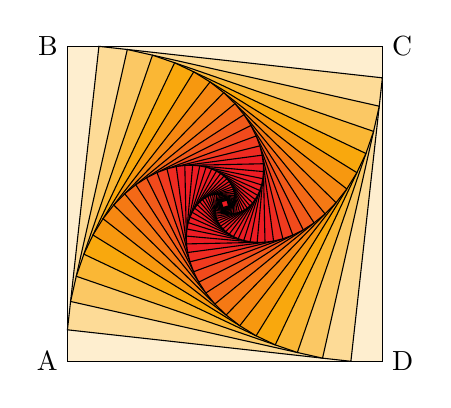
\begin{tikzpicture}
  \newcounter{density}
  \setcounter{density}{20}
  \def\couleur{Dandelion}
  \path[coordinate] (0,0) coordinate(A)
              ++( 90:4cm) coordinate(B)
              ++(0:4cm) coordinate(C)
              ++(-90:4cm) coordinate(D);
  \draw (A) node[left] {A}
    (B) node[left] {B}
    (C) node[right] {C}
    (D) node[right] {D};
  \draw[fill=\couleur!\thedensity] (A)--(B)--(C)--(D)--cycle;
  \foreach \x in {1,...,40}{%
      \pgfmathsetcounter{density}{\thedensity+25}
      \setcounter{density}{\thedensity}
      \path[coordinate] coordinate(X) at (A){};
      \path[coordinate] (A) -- (B) coordinate[pos=.1](A)
                          -- (C) coordinate[pos=.1](B)
                          -- (D) coordinate[pos=.1](C)
                          -- (X) coordinate[pos=.1](D);
      \draw[fill=\couleur!\thedensity] (A)--(B)--(C)--(D)--cycle;
  }
\end{tikzpicture}

  \caption{tikz例子}
  \label{fig:tikzrot}
\end{figure}

\begin{figure}[htb]
  \includegraphics[width=4cm]{nuaa-logo.pdf}
  \caption{一个校徽}
  \label{fig:logo}
\end{figure}

如果需要多个插图共用一个题注的话,需要加载额外的宏包,
一般选用 \pkg{subcaption} 或 \pkg{subfig},这两个宏包是互斥的。
需要注意的是 \pkg{subcaption} 貌似与 \pkg{geometry} 有些冲突,
会导致多行的图表的最后一行无法居中,而 \pkg{geometry} 是设置页边距的必用宏包。
所以个人推荐使用  \pkg{subfig},效果可以参考\autoref{fig:sub2}。

\begin{figure}[htb]
  \subfloat[左边的大校徽\label{fig:sub1}]{\includegraphics[width=4cm]{nuaa-logo.pdf}}\quad
  \subfloat[短标题:小校徽][小校徽,题注很长,不过请各位放心,它会自动换行\label{fig:sub2}]
  {\includegraphics[width=3cm]{nuaa-logo.pdf}}
  \caption{包含两张图片的插图}
  \label{fig:subfigs}
\end{figure}

如果需要插入图表的话,可以考虑使用 \pkg{pgfplots} 宏包,效果参见\autoref{fig:plots};
也可以用 Matplotlib、MatLab、Mathematica 之类的工具导出成兼容格式的图片。

\begin{figure}[htb]
  \subfloat[二维图像\label{fig:func}]{%\documentclass{ctexart}
%\usepackage{pgfplots}
%\pgfplotsset{compat=1.16}
%\begin{document}
\begin{tikzpicture}
  \pgfplotstableread[
    % col sep=comma
  ]{data/plot_2d.csv}{\Data}
  \begin{axis}[
    width=.45\textwidth,
    xmin=0, xmax=16, xtick distance=4,
    xlabel={序列},
    ymin=0, ymax=1,
    ylabel={正确率},
    grid=both,
    legend pos=south east,
  ]
    \addplot+ table[x=idx, y=parray] {\Data};
    \addlegendentry{环境1};
    \addplot+[mark=o] table[x=idx, y=pround] {\Data};
    \addlegendentry{环境2};
  \end{axis}
\end{tikzpicture}
%\end{document}
} \quad
  \subfloat[三维图像\label{fig:sum}]{%\documentclass{minimal}
%\usepackage{pgfplots}
%\pgfplotsset{compat=1.16}
%\begin{document}
\begin{tikzpicture}
  \pgfplotstableread[
    % col sep=comma
  ]{data/plot_3d.csv}{\Data}
  \begin{axis}[
    width=.45\textwidth,
    view={-30}{30},
    xmin=0, xmax=16, xtick distance=4,
    xlabel={Num},
    ymin=1, ymax=20, ytick distance=5,
    ylabel={Round},
    zmin=0, zmax=1, ztick distance=.2,
    zlabel={PDF},
    z tick label style={
      /pgf/number format/.cd,
        fixed,
        fixed zerofill,
        precision=1,
      /tikz/.cd
      },
    grid=major,
  ]
    \addplot3[
      surf,
      mesh/rows=17,
      patch type=rectangle,
      opacity=1,fill opacity=0.1,
      colormap/cool
    ] table[x=num, y=round, z=p] {\Data};
  \end{axis}
\end{tikzpicture}
%\end{document}
}
  \caption{拙作中利用 \pkg{pgfplot} 绘制的图表}
  \label{fig:plots}
\end{figure}

如果真的需要让十几张图片共用一个题注的话,
需要手工拆分成多个 \env{float} 并用 \cs{ContinuedFloat} 来拼接,
不过直接多次使用 \cs{caption} 会在图表清单里产生多个重复条目,需要一点点小技巧
(设置图表目录标题为空)。
建议将浮动位置指定为 \verb|t|,以确保分散至多页的图能占用整个页面,手工分页才能靠谱。
效果可以参见\autoref{fig:subfigss} 的\autoref{fig:logo6}。

\begin{figure}[t]
  \subfloat[校徽$\times 1$]{\includegraphics[width=4cm]{nuaa-logo.pdf}}\quad
  \subfloat[校徽$\times 2$]{\includegraphics[width=.4\textwidth]{nuaa-logo.pdf}}\\
  \subfloat[校徽$\times 3$]{\includegraphics[width=.4\textwidth]{nuaa-logo.pdf}}\quad
  \subfloat[校徽$\times 4$]{\includegraphics[width=4cm]{nuaa-logo.pdf}}
  \caption{包含多张图片的插图}
  \label{fig:subfigss}
\end{figure}
\begin{figure}[t]
  \ContinuedFloat
  \subfloat[校徽$\times 5$]{\includegraphics[width=4cm]{nuaa-logo.pdf}}\quad
  \subfloat[校徽$\times 6$ \label{fig:logo6}]{\includegraphics[width=4cm]{nuaa-logo.pdf}}\\
  \subfloat[校徽$\times 7$]{\includegraphics[width=4cm]{nuaa-logo.pdf}}\quad
  \subfloat[校徽$\times 8$]{\includegraphics[width=4cm]{nuaa-logo.pdf}}
  % 指定图表清单中的标题为[],即可将其消除,避免目录中出现重复条目
  \caption[]{包含多张图片的插图(续)}
\end{figure}

如果需要插入一张很大的图片的话,可以使用 \pkg{rotating} 提供的 \env{sidewaysfigure},
它能将插图放置在单独的页面上,如果文档使用 \verb|twoside| 选项的话,它会根据页面方向,
设置 \ang{90} 或 \ang{270} 旋转,可能需要编译两遍才能设置正确的旋转方向。
不过可能有一个问题,\env{sidewaysfigure} 中使用 \cs{subfloat} 可能无法准确标号,
需要手工重置 \texttt{subfigure} 计数器。
效果参见\autoref{fig:fullpage1} 和\autoref{fig:fullpage2}。

\setcounter{subfigure}{0}
\begin{sidewaysfigure}
  \subfloat[First caption\label{fig:fp1}]{\includegraphics[width=.8\textheight]{nuaa-jianqi.pdf}} \\
  \subfloat[Second caption]{\includegraphics[height=2cm]{nuaa-jianqi.pdf}}
  \caption{一幅占用完整页面的图片}
  \label{fig:fullpage1}
\end{sidewaysfigure}

\setcounter{subfigure}{0}
\begin{sidewaysfigure}
  \subfloat[First caption]{\includegraphics[height=2cm]{nuaa-jianqi.pdf}} \\
  \subfloat[Second caption]{\includegraphics[width=.8\textheight]{nuaa-jianqi.pdf}}
  \caption{又一幅占用完整页面的图片}
  \label{fig:fullpage2}
\end{sidewaysfigure}

\section{表格}

由于封面页,本模板预先加载了 \pkg{array} 和 \pkg{tabu},如果需要其他表格的宏包,
请自行加载。

如果需要插入一个简易的表格,可以只使用 \env{tabular} 环境,如\autoref{tab:city}。
\begin{table}[htb]
  \caption[城市人口]{城市人口数量排名 (source: Wikipedia)\label{tab:city}}
  \begin{tabular}{lr}
    \toprule
    城市 & 人口 \\
    \midrule
    Mexico City & 20,116,842\\
    Shanghai & 19,210,000\\
    Peking & 15,796,450\\
    Istanbul & 14,160,467\\
    \bottomrule
  \end{tabular}
\end{table}

也可以使用 \env{tabu} 环境,它可以更灵活地设置列宽,但它有一些 bug,如\autoref{tab:tabu}。
\begin{table}[htb]
  \caption{\env{tabu} 注意事项 \label{tab:tabu}}
  \begin{tabu} to .9\textwidth {XX[2]<{\strut}} \toprule
    默认列 & 有修正的列 \\ \midrule
    \env{tabu} 的 bug? \par This line is BAD & 注意左侧最后一行后的垂直空格 \\ \midrule
    注意对比最后一行 &
      bug 会影响多行的 \env{tabu} 表格 \par
      bug 的修正方法是在段落后面加 \cs{strut} \par
      This line is Good \\ \midrule
    垂直居中没效果 & 改用 \env{tabular} \\ \midrule
    与新版 \pkg{array} 不兼容 & 谨慎使用,切勿用 \texttt{tabu spread} \\ \bottomrule
  \end{tabu}
\end{table}

如果需要对某一列的小数点对齐,或者带有单位,或者需要做四舍五入的处理,可以尝试配合 \pkg{siunitx} 一起使用。
非常推荐看一下 \pkg{siunitx} 文档的,至少看一下“Hints for using siunitx”一节的输出结果,
\autoref{tab:xmpl:mixed} 来自于该文档的 7.14 节。

\begin{table}[htb]
  \caption{Tables where numbers have different units}
  \label{tab:xmpl:mixed}
  \begin{tabular}
    {
      >{$}l<{$}
      S[table-format = 2.3(1)]
      S[table-format = 3.3(1)]
    }
    \toprule
      & {One} & {Two} \\
    \midrule
    a / \si{\angstrom}   &  1.234(2) &   5.678(4) \\
    \beta / \si{\degree} & 90.34(4)  & 104.45(5)  \\
    \mu / \si{\per\mm}   &  0.532    &   0.894    \\
    \bottomrule
  \end{tabular}
  \hfil
  \begin{tabular}
    {S[table-format=1.3]@{\,}s[table-unit-alignment = left]}
    \toprule
    \multicolumn{2}{c}{Heading} \\
    \midrule
    1.234 & \metre   \\
    0.835 & \candela \\
    4.23  & \joule\per\mole \\
    \bottomrule
  \end{tabular}
\end{table}

如果表格内容很多,导致无法放在一页内的话,需要用 \env{longtable} 或 \env{longtabu} 进行分页。
\autoref{tab:performance} 是来自 \cquthesis{} 的一个长表格的例子。

\begin{longtable}[c]{c*{6}{r}}
	\caption[实验数据]{实验数据,这个题注十分的长,注意这在索引中的处理方式,还有 \cs{caption} 后面的双反斜杠}\label{tab:performance}\\
	\toprule
	\multirow{2}{*}{测试程序} & \multicolumn{1}{c}{正常运行} & \multicolumn{1}{c}{同步} & \multicolumn{1}{c}{检查点} & \multicolumn{1}{c}{卷回恢复}
	& \multicolumn{1}{c}{进程迁移} & \multicolumn{1}{c}{检查点} \\
	& \multicolumn{1}{c}{时间 (s)}& \multicolumn{1}{c}{时间 (s)}&
	\multicolumn{1}{c}{时间 (s)}& \multicolumn{1}{c}{时间 (s)}& \multicolumn{1}{c}{时间 (s)}& \multicolumn{1}{c}{文件 (KB)} \\ \midrule
	\endfirsthead
	\multicolumn{7}{c}{\nuaafontcaption 续表~\thetable\hskip1em 实验数据}\\
	\toprule
	\multirow{2}{*}{测试程序} & \multicolumn{1}{c}{正常运行} & \multicolumn{1}{c}{同步} & \multicolumn{1}{c}{检查点} & \multicolumn{1}{c}{卷回恢复}
	& \multicolumn{1}{c}{进程迁移} & \multicolumn{1}{c}{检查点} \\
	& \multicolumn{1}{c}{时间 (s)}& \multicolumn{1}{c}{时间 (s)}&
	\multicolumn{1}{c}{时间 (s)}& \multicolumn{1}{c}{时间 (s)}& \multicolumn{1}{c}{时间 (s)}& \multicolumn{1}{c}{文件(KB)} \\ \midrule
	\endhead
	\hline
	\multicolumn{7}{r}{续下页}
	\endfoot
	\endlastfoot
	CG.A.2 & 23.05 & 0.002 & 0.116 & 0.035 & 0.589 & 32491 \\
	CG.A.4 & 15.06 & 0.003 & 0.067 & 0.021 & 0.351 & 18211 \\
	CG.A.8 & 13.38 & 0.004 & 0.072 & 0.023 & 0.210 & 9890 \\
	CG.B.2 & 867.45 & 0.002 & 0.864 & 0.232 & 3.256 & 228562 \\
	CG.B.4 & 501.61 & 0.003 & 0.438 & 0.136 & 2.075 & 123862 \\
	CG.B.8 & 384.65 & 0.004 & 0.457 & 0.108 & 1.235 & 63777 \\
	MG.A.2 & 112.27 & 0.002 & 0.846 & 0.237 & 3.930 & 236473 \\
	MG.A.4 & 59.84 & 0.003 & 0.442 & 0.128 & 2.070 & 123875 \\
	MG.A.8 & 31.38 & 0.003 & 0.476 & 0.114 & 1.041 & 60627 \\
	MG.B.2 & 526.28 & 0.002 & 0.821 & 0.238 & 4.176 & 236635 \\
	MG.B.4 & 280.11 & 0.003 & 0.432 & 0.130 & 1.706 & 123793 \\
	MG.B.8 & 148.29 & 0.003 & 0.442 & 0.116 & 0.893 & 60600 \\
	LU.A.2 & 2116.54 & 0.002 & 0.110 & 0.030 & 0.532 & 28754 \\
	LU.A.4 & 1102.50 & 0.002 & 0.069 & 0.017 & 0.255 & 14915 \\
	LU.A.8 & 574.47 & 0.003 & 0.067 & 0.016 & 0.192 & 8655 \\
	LU.B.2 & 9712.87 & 0.002 & 0.357 & 0.104 & 1.734 & 101975 \\
	LU.B.4 & 4757.80 & 0.003 & 0.190 & 0.056 & 0.808 & 53522 \\
	LU.B.8 & 2444.05 & 0.004 & 0.222 & 0.057 & 0.548 & 30134 \\
	CG.B.2 & 867.45 & 0.002 & 0.864 & 0.232 & 3.256 & 228562 \\
	CG.B.4 & 501.61 & 0.003 & 0.438 & 0.136 & 2.075 & 123862 \\
	CG.B.8 & 384.65 & 0.004 & 0.457 & 0.108 & 1.235 & 63777 \\
	MG.A.2 & 112.27 & 0.002 & 0.846 & 0.237 & 3.930 & 236473 \\
	MG.A.4 & 59.84 & 0.003 & 0.442 & 0.128 & 2.070 & 123875 \\
	MG.A.8 & 31.38 & 0.003 & 0.476 & 0.114 & 1.041 & 60627 \\
	MG.B.2 & 526.28 & 0.002 & 0.821 & 0.238 & 4.176 & 236635 \\
	MG.B.4 & 280.11 & 0.003 & 0.432 & 0.130 & 1.706 & 123793 \\
	MG.B.8 & 148.29 & 0.003 & 0.442 & 0.116 & 0.893 & 60600 \\
	LU.A.2 & 2116.54 & 0.002 & 0.110 & 0.030 & 0.532 & 28754 \\
	LU.A.4 & 1102.50 & 0.002 & 0.069 & 0.017 & 0.255 & 14915 \\
	LU.A.8 & 574.47 & 0.003 & 0.067 & 0.016 & 0.192 & 8655 \\
	LU.B.2 & 9712.87 & 0.002 & 0.357 & 0.104 & 1.734 & 101975 \\
	LU.B.4 & 4757.80 & 0.003 & 0.190 & 0.056 & 0.808 & 53522 \\
	LU.B.8 & 2444.05 & 0.004 & 0.222 & 0.057 & 0.548 & 30134 \\
	EP.A.2 & 123.81 & 0.002 & 0.010 & 0.003 & 0.074 & 1834 \\
	EP.A.4 & 61.92 & 0.003 & 0.011 & 0.004 & 0.073 & 1743 \\
	EP.A.8 & 31.06 & 0.004 & 0.017 & 0.005 & 0.073 & 1661 \\
	EP.B.2 & 495.49 & 0.001 & 0.009 & 0.003 & 0.196 & 2011 \\
	EP.B.4 & 247.69 & 0.002 & 0.012 & 0.004 & 0.122 & 1663 \\
	EP.B.8 & 126.74 & 0.003 & 0.017 & 0.005 & 0.083 & 1656 \\
	\bottomrule
\end{longtable}

\section{数字与国际单位}

本模板预加载 \pkg{siunitx} 来格式化文中的内联数字,该宏包有大量可定制的参数,
请务必阅读其文档,并在文档导言部分设置格式。

\begin{itemize}
  \item 旋转角度为 \ang{90}、\ang{270}
  \item 分辨率 \num{1920x1080} 的像素数量约为 \num{2.07e6}
  \item 电脑显示器的像素间距为 \SI{1.8}{\nm}、\SI{180}{\um} 还是 \SI{18}{\mm}?
  \item 重力加速度 $g=\SI{9.8}{\kg\per\square\second}$、
  $g=\SI[inter-unit-product=\ensuremath{{}\cdot{}}]{9.8}{\kg\per\square\second}$,
  亦或 $g=\SI[per-mode=symbol]{9.8}{\kg\per\square\second}$
\end{itemize}

\section{中英文之间空格}

很遗憾,目前 \LaTeX{} 和 \CTeX{} 虽然能处理普通汉字与英文之间的间隔,
但是汉字与宏之间的空格仍然需要手工调整,请务必按以下的规则撰写原稿:
\begin{itemize}
  \item[\ding{51}] 如\autoref{fig:sub2} 所示:\verb|如\autoref{fig:sub2} 所示|,这个宏返回的是“图 x.xx”,
  所以前面两个汉字之间不能加空格,后面数字与汉字之间必须加空格;
  \item[\ding{51}] 距离为 1.7~个天文单位:\verb|距离为 1.7~个天文单位|,前面可以不加空格(\CTeX 会修正),
  后面必须加 \verb|~| 以防止在 “1.7”与“个”之间换行。此时更推荐写成 \SI{1.7}{au}:\verb|\SI{1.7}{au}|。
\end{itemize}


\appendix
% 如果需要附录的话,在这里 include
%\chapter{后记}

\section{v0.9a后记——Old Jack 的吐槽}

\verb!\begin{轻松+愉快}!

Old Jack 他有点累......

Old Jack 两年前就开始关注南航毕设的\LaTeX 模板了,但是两年了还没有任何有实际意义的新动作,所以Old Jack 就亲自操刀制作了新的一版。虽然很多代码都是从其他模板中直接摘抄过来的,但是这也是\TeX 最普遍、最快捷的学习\&开发方法。一开始 Old Jack 也想造轮子,但是轮子真的不好造。

在制作过程中遇到了几个关键性的问题:
\begin{itemize}
  \item 前文提到的三种粗体
  \item nuaa.png源文件和页眉制作
  \item 英文字母、章节标题莫名其妙的加粗
  \item 脚注相对页脚线的位置
\end{itemize}

第一个问题 Old Jack 曾经用\TeX 中伪粗体(FakeBold)的方法实现过,但是效果并不好,而且当时受到最后一个问题的强烈影响,不得不使用其他字体来解决这个问题。

第二个问题 Old Jack 开始是使用官方模板中的图片,但是分辨率太低,效果很差。于是 Old Jack Google以图搜图找到了现在的这个文件的源文件,经过了一系列不可描述的操作后得到了现在的 nuaa.png 。页眉的制作也让 Old Jack 很头疼,论文要求论文到顶端和底端的距离分别为2.5cm和2.0cm,Old Jack 很naive的就给geometry设置了这个数值,但是效果和官方模板差了很多,于是 Old Jack 只好一点一点地调试,达到了近似官方模板的效果。页脚和官方模板有细微的区别,Old Jack 认为这无伤大雅,是要罗马数字和阿拉伯数字编号正确应该就可以了。

第三个问题是一个非常奇怪的问题。使用伪粗体时所有标题全都加粗了,非常难看,经过了代码重构和不停地调试解决了这个问题。在模板完成99\% 后发现最后致谢中的英文字体全都加粗了, Old Jack 几次审视代码和调试都没有解决。偶然间,Old Jack 将全部主要文件全部提取出来,放入另一个文件夹,然后重新编译就解决了这个问题!当然后来发现代码中确实有一个地方有小问题\textbf{可能}会影响,但是这不是上一次出错的原因。Old Jack 对于各位使用模板的南航学子以及其他可能会参考此模板的\TeX 爱好者提了一个建议:\textbf{任何语言,任何代码出现莫名其妙的问题时,换一个文件夹,改一下名字,重新跑一下,可能会得到意想不到的结果。}当然这不是万能的解决方法。

第四个问题就如第一章中脚注和页脚线的情况,感觉两条线很别扭。 Old Jack 犹豫了很久,最后没有采用将脚注放在页脚线下的方案,因为 Old Jack 觉得还是两条线的方案好看。对于想要将脚注放在页脚线下方的同学,可以在主文件中取消注释那段代码,来实现所需要的效果。

Old Jack 他完成了模板的再制作,但是他没有心气再写出一篇能够指导大家使用\LaTeX 的文档了(好吧,Old Jack 他承认懒是一部分因素),望大家谅解 Old Jack。

\verb!\end{轻松+愉快}!

\section{v1.0后记}

Old Jack 非常高兴,因为他不是一个人在战斗。再次感谢张一白、王成欣、曾宪文、Gavin Lee等人的工作,没有他们,\nuaathesis 不会像现在这么美丽。

经过\nuaathesis~Group的努力和测试,\nuaathesis 迎来了v1.0版,也就是第一个正式发行版。一路走来也是有些坎坷,各种各样的小问题一直困扰着我们,其实v1.0 也还有着一些细小的问题尚未解决。不过Old Jack请大家放心,这些小问题不影响模板的使用。很多已经被我们解决的小问题比如页眉的大小位置,中英文字体是否正确,摘要的章节标题不能是加粗的宋体等等,老师可能不去管这些,甚至注意不到有什么区别。相比之下,重要的地方是:公式、图表的编号,图表和文本的位置,参考文献的格式等等才是老师关注的点。很多地方只是我们几个人为了追求和office模板尽可能接近,才不断地进行修改调整,也是有点讽刺。

写毕设论文的时候,Old Jack 不止一次看到隔壁室友调公式内容,Mathtype和Office装了卸,卸了装、调公式编号、调标题位置和大小、调首行缩进、调段间距等等等等,看着他们搞得焦头烂额的,Old Jack 都觉得心累。打印时也是这样,有太多的人在打印店不停地修改自己的论文,有因为office和wps不兼容修改的,有office版本不兼容修改的,有因为页眉页脚错误修改的等等。然而 Old Jack 他在写论文时从来没有担心过这些事情(当然,作为模板开发者 Old Jack 确实操心了很多,2333),他也第一次真正体会到了什么叫做专注于内容,真的挺轻松的(表格是例外)。

对于模板的推广,Old Jack觉得使用人数仍然不会太多,毕竟\LaTeX 的群众基础太小,除了8院,其他学院对公式的需求整体来讲并不迫切,Old Jack 猜测大部分知道、了解\LaTeX 的同学是通过数学建模竞赛这个途径才学习了\LaTeX ;同时因为涉及到学习新的程序语言,时间成本也较大,所以很多同学的学习意愿不高。不过\nuaathesis 的目标人群本来也不是全校所有学生,Old Jack 的思路,Old Jack 相信也是\nuaathesis~Group其他开发者的思路是:
\begin{enumerate}
  \item 为自己服务,这是\nuaathesis~Group开发模板的第一动力;
  \item 对已经掌握\LaTeX 基本语法的同学,\nuaathesis~Group为他们在毕业设计时能更轻松地撰写论文,提供平台和机会;
  \item 对准备学习\LaTeX 以及已经学习了一点\LaTeX 的同学,\nuaathesis~Group为他们提供学下去的动力和平台。
\end{enumerate}

即将毕业了,回首大学四年, Old Jack 做过疯狂的事情,也找到了一份看起来还可以的工作,只觉得还没对学校做过什么有用的事情,尽管 Old Jack 对学校其实并不是很有感情。完成了这个模板后,至少 Old Jack 可以减少一个遗憾,然后离开学校了。虽然这不是什么惊天动地的工作,但是至少 Old Jack 做了件他认为还算有意义的事情。Old Jack应该还会再维护\nuaathesis 一段时间,期待有后继者能够接过火炬,继续完善并推广\nuaathesis 。

想说的可能也就这么多了,Old Jack out!

\hfill 0813~王志浩,2017.6.24

\section{v2.0 后记 by yzwduck}

也是两年前开始关注南航毕设的\LaTeX 模板了,但直到毕业前,都没能去静下心来学习\LaTeX。

现在差不多本科毕业一年,或者说,一年后要开写硕士学位论文了,
本打算照着 CQUThesis 来造轮子的时候,逛纸飞机\footnote{论坛还活着吗?该不会已经沦落为老人的回忆了吧。 ——2018.10.10}
看到 \nuaathesis~v1.0 发布了。
非常激动、也很自愧,同样是经历了大学四年的人,我没能把这模板做出来。

于是马上把两年前为了模板而画的校名(矢量图)传了上去\footnote{\url{https://github.com/nuaatug/nuaathesis/commit/24fa82e}}。

原本打算在 v1.0 版的基础上修改的,但因为行间距设置有问题,封面与 Word 模板也有点差异,
还要再加入硕/博士的模板,于是干脆改成 \texttt{Documented LaTeX Source (.dtx)},
方便以后写模板的文档。

做模板过程中遇到的大问题,在于如何正确理解学校对论文格式的要求。
虽然有《本科毕业设计(论文)撰写格式要求》、《研究生学位论文撰写要求》,
但这些要求依然不够细致,因为那些要求都是假定你用 Word 来写论文的,要求里的内容是 Word 设置的操作方法,
所以还要先学习 Word 的排版算法。虽然这不是热门的资料,而且还有 CJK 独有的坑,
幸好有人把 Word 排版算法解释得非常详细,这个模板才能避免大量使用测量得到的魔数。
但还有很多细节部分,因为能力有限,没能实现。

最后容我吐槽一下学校的 Word 模板,我觉得那个 Word 模板可能从最初做出来后,就基本没有变化。
那个“最初”或许可以追溯到上个世纪。很多编号的事情都要由手工来完成,比如说目录页码、
各级标题的编号、题注等。这些完全可以自动编号的工作,如果要手工做的话【掀桌颜文字】。

\section{v2.1 后记 by yzwduck}

转眼间一年过去,又到了写毕业论文的时候了。

翻了一下代码的 commit 记录(部分非公开),这一年间只有加起来两、三个星期在做这个论文模板,
已经无法用“懒”这字来描述鄙人的状态了。

不过也有几件值得小小炫耀一下的事,终于把中/英/日多国语的坑填了不少,至少能编译出对应语言的论文来;
为了减少重复代码,使用一些宏包造了 \CTeX{} 的几个轮子,从而实现一个 class 文件能支持三国语言。

为了检验模板的效果,鄙人从知网上找了两篇论文,试着用 \nuaathesis{} 模板排版了一下(节选),又发现了不少问题。
因此目前 \nuaathesis{} 应该还有相当多的问题的,但没有用户的话,由于鄙人能力有限,难以发现,
还请各位使用 \nuaathesis{} 的先行者们(Pioneers) 能反馈意见和建议。

愿所有使用 \nuaathesis{} 的人,不会被评审老师指责格式问题。


\backmatter
% 如果参考文献使用 biber
\bibliographystyle{nuaabib}   % 参考文献的样式
\bibliography{bib/sample}   % 参考文献,即 bib/sample.bib 文件(纯文本)
% 如果打算手写参考文献
%\chapter{\bibname}

\begin{manref}
\item \label{ref:hint} 手作りの参考文献
\item \zhcn{如果能使用 biber,就不要手写参考文献}
\item \zhcn{如果一定要手写的话,就按照学校的参考文献格式来写,如:}
\item \label{ref:man} KANAMORI H. Shaking without quaking[J]. Science, 1998, 279(5359): 2063.
\end{manref}

例:[\ref{ref:hint}]はヒントです、\mcite{ref:man}は1998年に発表されました。


\chapter[致谢]{致\hskip\ccwd{}谢}

在此感谢对本论文作成有所帮助的人。

\chapter{在学期间的研究成果及学术论文情况}

% 不要在意为什么没有 section,因为只是套用一下格式

\subsection*{攻读硕士学位期间发表(录用)论文情况}

\begin{enumerate}
  \item Kaiwen Cai,Zhiquan Deng,Cong Peng,Kexiang Li. Suppression of Harmonic Vibration in Magnetically Suspended Centrifugal Compressor Using Zero-Phase Odd-Harmonic Repetitive Controller. IEEE Transactions on Industrial Electronics. In early access. 2019.09.
  \item Kaiwen Cai,Zhiquan Deng,Cong Peng,Kexiang Li. Vibration Suppression Control for MSFW with Gyroscopic Effects Using Synchronous Rotate Frame. 37th China Control Conference.
  \item Cong Peng, Kaiwen Cai, Zhiquan Deng. Vibration Torque Suppression for Magnetically Suspended Flywheel Using Improved Synchronous Rotating Frame Transformation, Shock and Vibration.2019.
\end{enumerate}

\subsection*{攻读硕士学位期间发表(录用)专利情况}

\begin{enumerate}
  \item 彭聪,蔡凯文,邓智泉,基于交叉解耦陷波方法的同频振动力矩抑制控制方法,授权发明专利CN107807533B,2019.08.20。
\end{enumerate}

\subsection*{研究生期间参与的科研项目}

\begin{enumerate}
  \item 校企合作项目“高速磁悬浮空气压缩机的磁悬浮轴承技术研究”。
\end{enumerate}






\end{document}
